% !TEX root = ../main.tex
% ============================================================
%  CAPÍTULO 3 — INGENIERÍA DEL PROYECTO
%  Proyecto: Sistema de monitoreo de consumo de combustible
%            por protocolo CAN OBD-II
% ============================================================

\chapter{INGENIERÍA DEL PROYECTO}

% ────────────────────────────────────────────────────────────
\section{Descripción general del sistema}
% Sin cambios respecto a tu versión actual.
% Incluye: subsistemas funcionales + diagrama de arquitectura.
El sistema propuesto tiene como uno de los objetivos principales optimizar el consumo energético, limitando el uso de componentes innecesarios y priorizando la eficiencia del sistema embebido. Debido a que la fuente de alimentación proviene directamente de la batería del vehículo, un consumo excesivo de energía podría ocasionar la descarga de la misma, afectando el arranque y funcionamiento del automóvil.

Con el propósito de mejorar la organización, modularidad y escalabilidad del diseño, el sistema se divide en los siguientes subsistemas funcionales:

\begin{itemize}
	\item \textbf{Sistema de protección eléctrica.} Etapa de aislamiento analógico encargada de salvaguardar los componentes lógicos frente a transitorios de tensión, picos de sobrecorriente, inversión de polaridad y ruido electromagnético (EMI) inherente a la red del vehículo.
	
	\item \textbf{Sistema de alimentación.} Módulo de acondicionamiento de potencia que convierte la tensión nominal de 12~V extraída del puerto OBD-II a niveles lógicos estables (ej. 3.3~V o 5~V) mediante regulación DC-DC.
	
	\item \textbf{Sistema de adquisición de datos.} Capa física (\textit{PHY}) acoplada a las líneas diferenciales CAN~High y CAN~Low (pines 6 y 14 del conector OBD-II) para la intercepción, lectura y transmisión de las tramas de diagnóstico del automóvil.
	
	\item \textbf{Sistema de procesamiento y filtrado.} Etapa algorítmica donde el firmware central extrae la carga útil (\textit{payload}) de los mensajes de red, descartando el ruido o tramas irrelevantes y decodificando los PIDs hexadecimales a valores físicos operables.
	
	\item \textbf{Sistema de cálculo y control.} Subsistema lógico que aplica modelos estequiométricos de dinámica de fluidos utilizando los parámetros extraídos (como flujo de aire y RPM) y la retroalimentación del sensor lambda para estimar la tasa real de consumo de combustible.
	
	\item \textbf{Sistema de almacenamiento de datos.} Unidad de gestión de memoria (\textit{datalogger}) que resguarda los registros en buffers temporales o memoria no volátil, garantizando la preservación de los históricos de conducción ante cortes de energía.
	
	\item \textbf{Sistema de interfaz de usuario (HMI).} Módulo de visualización en cabina que otorga retroalimentación directa de las variables calculadas e instrumentación en tiempo real, permitiendo la interacción física del conductor.
	
	\item \textbf{Plataforma de monitoreo web.} Servidor de interfaz de red (\textit{Dashboard}) diseñado para la recepción, graficación y análisis remoto de los datos telemétricos del vehículo.
\end{itemize}

Teniendo finalmente un diagrama ver Figura \ref{fig:arquitectura_final_limpia}

\begin{figure}[H]
	\centering
	\captionsetup{labelformat=simple, labelsep=newline, textfont=it, labelfont=bf}
	\caption{Diagrama de bloques de la arquitectura funcional y flujo de señales del sistema}
	\label{fig:arquitectura_final_limpia}
	\vspace{0.4cm}
	
	\shorthandoff{<>}
	
	\resizebox{\textwidth}{!}{%
		\begin{tikzpicture}[
			>=Stealth,
			node distance=1.3cm and 1.4cm,
			block/.style={rectangle, draw, fill=blue!5, text width=4.3cm, text centered, rounded corners, minimum height=1.5cm, font=\small},
			mcu_block/.style={rectangle, draw, fill=green!5, text width=4.1cm, text centered, rounded corners, minimum height=1.4cm, font=\small},
			ext_block/.style={rectangle, draw, fill=gray!10, text width=4.6cm, text centered, rounded corners, minimum height=1.5cm, font=\small},
			line/.style={draw, ->, thick},
			bi_line/.style={draw, <->, thick},
			pwr_line/.style={draw, ->, thick, red, dashed}
			]
			
			% Nodos
			\node[ext_block] (obd) {\textbf{Conector OBD-II}\\(Vehículo Changan Honor)};
			\node[block, below=1.5cm of obd] (adquisicion) {\textbf{3. Adquisición}\\(Transceptor SN65HVD230)};
			\node[mcu_block, below=1.9cm of adquisicion] (procesamiento) {\textbf{4. Procesamiento}\\(Controlador CAN TWAI)};
			\node[mcu_block, below=1.6cm of procesamiento] (calculo) {\textbf{5. Cálculo y Control}\\(Algoritmo Consumo)};
			
			\node[block, left=1.8cm of adquisicion] (proteccion) {\textbf{1. Prot. Eléctrica}\\(Filtro EMI y Fusible)};
			\node[block, below=1.6cm of proteccion] (alimentacion) {\textbf{2. Alimentación}\\(Regulador DC-DC a 3,3V)};
			
			\node[mcu_block, right=1.8cm of procesamiento] (almacenamiento) {\textbf{6. Almacenamiento}\\(Memoria \textit{Datalogger})};
			\node[mcu_block, right=1.8cm of calculo] (comunicacion) {\textbf{7. Comunicación}\\(Wi-Fi / BT Nativo)};
			
			\node[ext_block, below=1.8cm of calculo] (hmi) {\textbf{8. Interfaz de Usuario}\\(Pantalla HMI / LCD)};
			\node[ext_block, fill=cyan!5, right=1.8cm of hmi] (web) {\textbf{9. Monitoreo Web}\\(\textit{Dashboard} Remoto)};
			
			% Contenedor
			\begin{scope}[on background layer]
				\node[draw, black!40, dashed, thick, fill=green!2, rounded corners, fit=(procesamiento) (calculo) (almacenamiento) (comunicacion), inner sep=0.6cm, inner ysep=0.8cm] (mcu_group) {};
				\node[above left=0.05cm and 0.1cm of mcu_group.north east, font=\bfseries\small, text=black!60] {Capa de Firmware (SoC ESP32)};
			\end{scope}
			
			% Conexiones
			\draw[pwr_line] (obd.west) -| (proteccion.north) node[pos=0.3, above, font=\scriptsize, text=black] {12V DC};
			\draw[pwr_line] (proteccion) -- (alimentacion);
			\draw[pwr_line] (alimentacion.east) -- (procesamiento.west) node[midway, above, font=\scriptsize, text=black] {3.3V};
			
			\draw[line] (obd) -- (adquisicion) node[midway, right, font=\scriptsize] {CAN H / CAN L};
			\draw[line] (adquisicion) -- (procesamiento) node[midway, right, font=\scriptsize] {Líneas TX/RX};
			\draw[line] (procesamiento) -- (calculo) node[midway, right, font=\scriptsize] {PIDs Raw};
			
			\draw[line] (procesamiento.east) -- (almacenamiento.west) node[midway, above, font=\scriptsize] {SPI / I2C};
			\draw[line] (calculo.east) -- (comunicacion.west) node[midway, above, font=\scriptsize] {Variables};
			
			\draw[line] (calculo) -- (hmi) node[midway, right, font=\scriptsize] {Bus Local};
			\draw[line] (comunicacion.south) -- (web.north) node[midway, right, font=\scriptsize] {HTTP / WS};
			
		\end{tikzpicture}%
	}
	\vspace{0.4cm}
	
	\begin{flushleft}
		\footnotesize \textit{Nota.} Arquitectura del sistema embebido. La columna izquierda procesa la etapa de potencia; la central gobierna el flujo del bus CAN y el núcleo del procesador; la derecha y la base gestionan el almacenamiento local y la telemática. Elaboración propia.
	\end{flushleft}
	
	\shorthandon{<>}
\end{figure}

% ────────────────────────────────────────────────────────────
\subsection{Configuración del entorno de captura}
% Conexión ESP32 + SN65HVD230 al conector OBD-II.
% Modo SLCAN, firmware serial bridge, SavvyCAN.
% Figura: diagrama de conexión de sniffing.
Para validar experimentalmente los fundamentos teóricos del protocolo CAN, se propone el desarrollo de un prototipo orientado a la captura y lectura de tramas de datos a través del puerto OBD-II. Este sistema requiere de una interfaz física capaz de realizar la transición entre el medio físico de transmisión y el nivel lógico digital. Dado que el protocolo CAN opera bajo un esquema de señalización diferencial a través de los hilos CAN-H y CAN-L, es indispensable integrar un transceptor que convierta dichas diferencias de potencial en niveles lógicos (TTL/CMOS) compatibles con un microcontrolador.

Este prototipo se fundamenta en los principios del hacking ético aplicado a sistemas automotrices \citep{ocsaly2022canfuzzer}, cuyo enfoque permite la extracción, monitoreo y análisis de datos vehiculares mediante el uso de hardware embebido. El flujo operativo de esta arquitectura de adquisición se ilustra en la Figura \ref{fig:flujo_logico_datos}.

\begin{figure}[H]
	\centering
	\captionsetup{labelformat=simple, labelsep=newline, textfont=it, labelfont=bf}
	\caption{Diagrama de flujo lógico para la adquisición y procesamiento de datos}
	\label{fig:flujo_logico_datos}
	\vspace{0.4cm}
	
	% Desactivar Babel temporalmente para el entorno
	\shorthandoff{<>}
	
	\resizebox{\textwidth}{!}{%
		\begin{tikzpicture}[
			node distance=2.0cm,
			% Usamos una sintaxis que no requiere < o >
			myarrow/.style={-{Stealth[scale=1.2]}, ultra thick, black!70},
			stage/.style={rectangle, draw, fill=gray!10, text width=3.8cm, text centered, rounded corners, minimum height=1.5cm, font=\small\bfseries},
			process/.style={rectangle, draw, fill=blue!5, text width=3.8cm, text centered, rounded corners, minimum height=1.5cm, font=\small\bfseries}
			]
			
			\node[stage] (bus) {Bus de Datos \\ Puerto OBD-II};
			\node[stage, right=of bus] (traductor) {Interfaz Física};
			\node[process, right=of traductor] (mcu) {Procesamiento\\Digital};
			\node[process, right=of mcu] (interpretacion) {Interpretación de Datos\\(Información Útil)};
			
			% Aquí usamos el estilo 'myarrow' definido arriba
			\draw[myarrow] (bus) -- (traductor) node[midway, above, font=\scriptsize] {};
			\draw[myarrow] (traductor) -- (mcu) node[midway, above, font=\scriptsize] {};
			\draw[myarrow] (mcu) -- (interpretacion) node[midway, above, font=\scriptsize] {};
			
		\end{tikzpicture}%
	}
	
	% Reactivar Babel
	\shorthandon{<>}
	\vspace{0.4cm}
	
	\begin{flushleft}
		\footnotesize \textit{Nota.} Esquema del flujo de información. Elaboración propia.
	\end{flushleft}
\end{figure}

Según \citet{ocsaly2022canfuzzer}, para la implementación de este tipo de sistemas se pueden emplear principalmente dos arquitecturas de interfaz. La primera consiste en el uso del controlador CAN MCP2515 en conjunto con el transceptor físico TJA1050. Por otra parte, está la alternativa basada en el transceptor SN65HVD230, que opera a un nivel de voltaje de 3{,}3V y por eso resulta directamente compatible con los microcontroladores de la serie ESP32, sin necesitar conversores de nivel externos.

En la Tabla \ref{tab:comparativa_arquitecturas} se detallan las ventajas y desventajas técnicas de ambas configuraciones, facilitando la selección de la arquitectura más eficiente para este desarrollo.

\begin{table}[h]
	% Ajuste para alinear a la izquierda
	\captionsetup{justification=raggedright, singlelinecheck=false, labelformat=simple, labelsep=newline, textfont=it, labelfont=bf}
	\caption{Comparativa técnica entre arquitecturas de adquisición CAN}
	\label{tab:comparativa_arquitecturas}
	
	\renewcommand{\arraystretch}{1.3}
	
	\resizebox{\textwidth}{!}{%
		\begin{tabular}{p{4.5cm} p{5.5cm} p{5.5cm}}
			\toprule
			\rowcolor[rgb]{0.851, 0.851, 0.851}
			\textbf{Característica} & \textbf{Opción A: MCP2515 + TJA1050 + ATmega328p} & \textbf{Opción B: SN65HVD230 + ESP32} \\
			\midrule
			Controlador CAN & Externo (MCP2515 vía SPI). & Interno (TWAI nativo en ESP32). \\
			\addlinespace
			Nivel de Tensión & 5V (requiere conversores si el MCU es 3{,}3V). & 3{,}3V (nativo, sin conversores). \\
			\addlinespace
			Complejidad & Alta (más componentes, más cableado). & Baja (arquitectura minimalista). \\
			\addlinespace
			Velocidad & Limitada por la interfaz SPI. & Alta (gestión directa por hardware). \\
			\addlinespace
			Eficiencia Energética & Consumo mayor por múltiples integrados. & Muy eficiente (modo Standby avanzado). \\
			\addlinespace
			Facilidad de Implementación & Requiere librerías externas de terceros. & Integración nativa con framework ESP-IDF. \\
			\bottomrule
		\end{tabular}%
	}
	\vspace{0.2cm}
	
	\begin{flushleft}
		\footnotesize \textit{Nota.} Comparativa entre la arquitectura clásica de 8 bits y la arquitectura SoC de 32 bits de alto rendimiento. Elaboración propia.
	\end{flushleft}
\end{table}

Finalmente, se ha seleccionado la Opción B para la implementación del sistema de adquisición de datos del bus CAN, la cual integra el transceptor SN65HVD230 con el microcontrolador ESP32. Esta elección se fundamenta en las ventajas técnicas expuestas en la Tabla \ref{tab:comparativa_arquitecturas} y en las recomendaciones metodológicas propuestas por \citet{ocsaly2022canfuzzer}.

\subsection{Esquema de conexión ESP32 -- OBD-II}
% Pinout OBD-II pines 6 (CANH) y 14 (CANL).
% Tabla: conexión ESP32 GPIO → SN65HVD230 → OBD-II.
Para establecer la comunicación entre el microcontrolador y la red CAN del vehículo, es necesario realizar una interconexión precisa entre el puerto OBD-II, el transceptor SN65HVD230 y el ESP32. El diseño del cableado debe garantizar la integridad de la señal diferencial y minimizar el ruido electromagnético.

\subsection{Interfaz con el puerto OBD-II}
La conexión al puerto de diagnóstico requiere la identificación exacta de los pines normalizados en el conector macho:
\begin{itemize}
	\item \textbf{Pin 6 (CAN-H):} Línea de señal diferencial alta.
	\item \textbf{Pin 14 (CAN-L):} Línea de señal diferencial baja.
	\item \textbf{Pin 5 (Signal Ground):} Masa de referencia para la señal de datos. Se recomienda estrictamente el uso del Pin 5 en lugar del Pin 4 (masa de chasis), debido a que este último suele presentar un alto nivel de ruido eléctrico derivado de los componentes auxiliares del vehículo, como el alternador o los limpiaparabrisas.
\end{itemize}

\subsection{Configuración del transceptor SN65HVD230}
El transceptor actúa como el puente físico para interpretar los niveles de tensión del bus CAN. Los cables provenientes del puerto OBD-II deben conectarse a los terminales correspondientes del módulo (H, L y GND). Es imperativo que las líneas CAN-H y CAN-L mantengan una configuración de \textbf{par trenzado} a lo largo de todo el cableado, ya que esta técnica permite la cancelación de interferencias electromagnéticas externas.

\subsection{Enlace lógico con el ESP32}
La comunicación digital entre el transceptor y el microcontrolador se realiza mediante el protocolo TWAI (\textit{Two-Wire Automotive Interface}) nativo del ESP32, siguiendo la configuración de pines descrita a continuación:
\begin{itemize}
	\item \textbf{VCC (3{,}3V):} Alimentación del módulo transceptor.
	\item \textbf{GND:} Punto de masa común; es fundamental que el ESP32, el transceptor y la señal de referencia proveniente del vehículo compartan una misma referencia a tierra.
	\item \textbf{CTRX/CRX (Transmisión/Recepción):} Conexión a los pines de entrada/salida (IO4 e IO5), configurados mediante el \textit{firmware} para la gestión de las tramas de datos.
\end{itemize}

\subsection{Consideraciones de montaje y seguridad}
Previo a la integración definitiva en el vehículo, se deben realizar las siguientes validaciones físicas:
\begin{itemize}
	\item \textbf{Prueba de tracción:} Verificar la solidez de todas las soldaduras mediante una tracción mecánica suave para asegurar conexiones estables.
	\item \textbf{Alivio de tensión:} Aplicar fijaciones mecánicas (como abrazaderas o adhesivo termofusible) en los puntos de entrada de los cables hacia los módulos para prevenir daños por tensión mecánica accidental.
\end{itemize}

Y finalmente mostramos en la Tabla \ref{tab:pinout_conexion} las conexiones.

\begin{table}[htbp]
	\centering
	\captionsetup{justification=raggedright, singlelinecheck=false, labelformat=simple, labelsep=newline, textfont=it, labelfont=bf}
	\caption{Esquema de conexiones (Pinout) entre el puerto OBD-II, el transceptor y el microcontrolador}
	\label{tab:pinout_conexion}
	\renewcommand{\arraystretch}{1.2}
	\begin{tabular}{p{3.5cm} p{3.5cm} p{5cm}}
		\toprule
		\rowcolor[rgb]{0.851, 0.851, 0.851}
		\textbf{Origen} & \textbf{Destino} & \textbf{Función/Nota} \\
		\midrule
		OBD-II Pin 6 & SN65HVD230 CAN-H & Señal diferencial alta. \\
		OBD-II Pin 14 & SN65HVD230 CAN-L & Señal diferencial baja. \\
		OBD-II Pin 5 & GND Común & Referencia a tierra (no usar Pin 4). \\
		SN65HVD230 VCC & ESP32 3{,}3V & Alimentación lógica del módulo. \\
		SN65HVD230 TX & ESP32 GPIO 4 & Transmisión de datos (TX). \\
		SN65HVD230 RX & ESP32 GPIO 5 & Recepción de datos (RX). \\
		\bottomrule
	\end{tabular}
	\vspace{0.2cm}
	\begin{flushleft}
		\small
		\begin{center}
			\textit{Nota.}Elaboración propia.
		\end{center}
		
	\end{flushleft}
\end{table}

En la Figura \ref{fig:obd_conector_soldado} se muestra el esquema de conexión:

\begin{figure}[h]
	\centering
	% El título y número se integran en el \caption (arriba de la imagen en APA)
	\caption{Esquema de conexión de los pines CAN-H y CAN-L al microcontrolador}
	\label{fig:obd_conector_soldado}
	
	\vspace{0.3cm}
	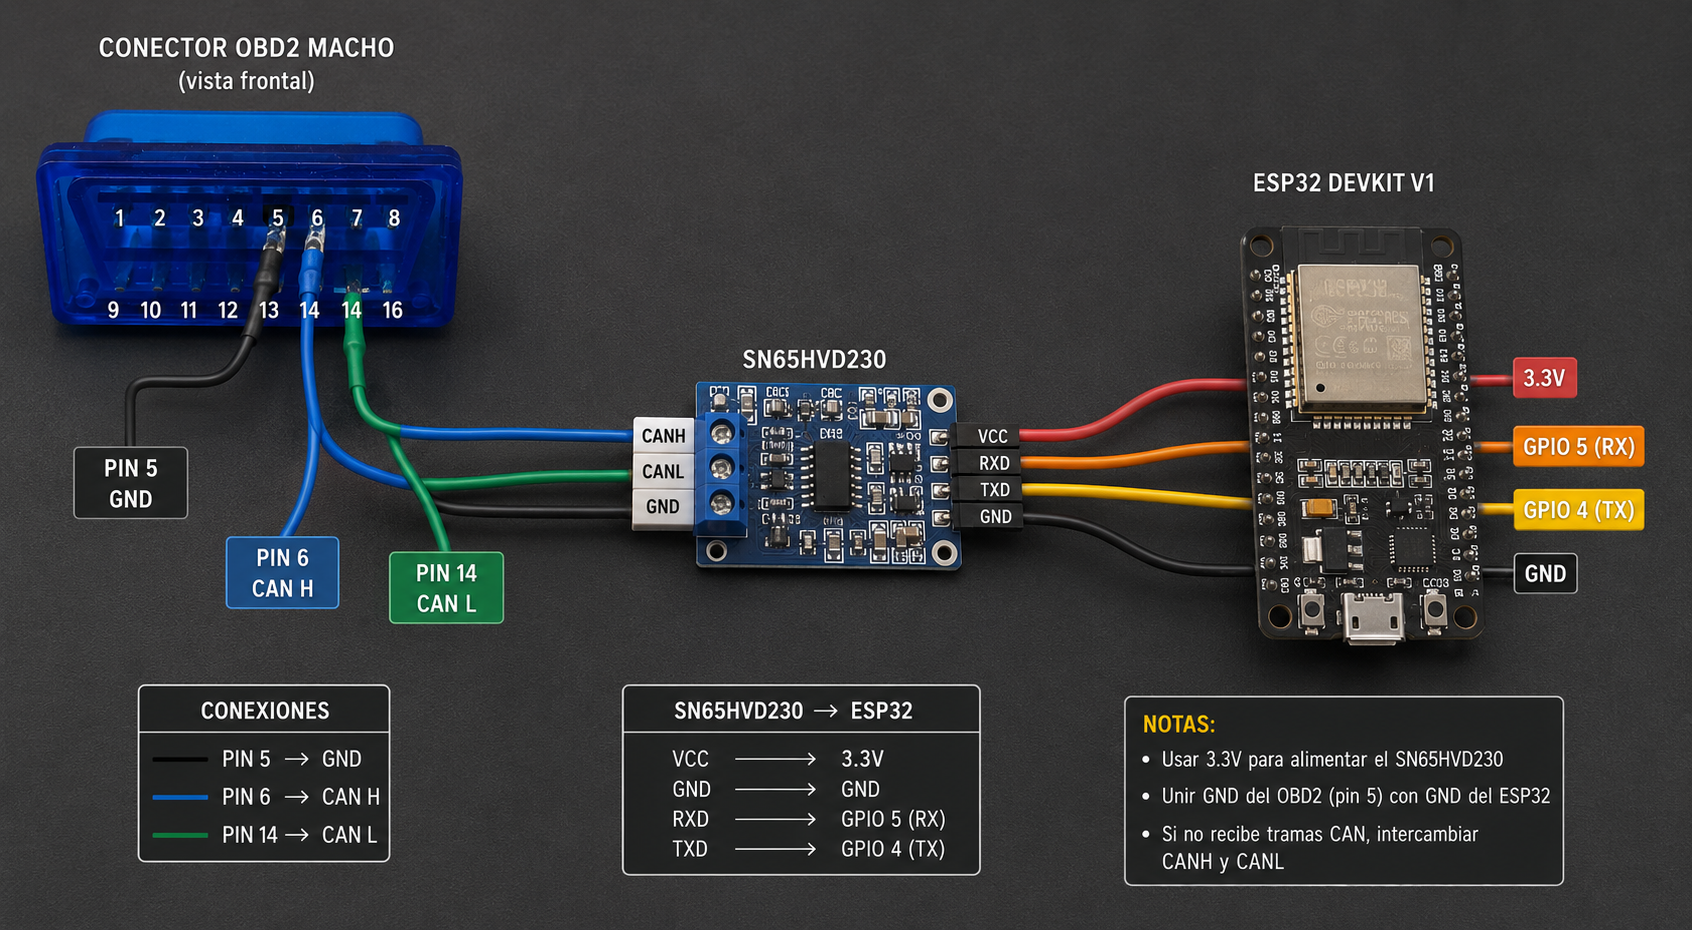
\includegraphics[width=1\textwidth]{Images/REAL.png}
	\vspace{0.2cm}
	
	% La nota explicativa detallada va debajo, alineada a la izquierda
	\begin{flushleft}
		\footnotesize \textit{Nota.} Esquema de conexión entre los componentes de la Tabla \ref{tab:pinout_conexion}. Elaboración propia asistida con IA (Gemini).
	\end{flushleft}
\end{figure}


\subsection{Configuración SLCAN y SavvyCAN para el análisis de datos}

Una vez completada la implementación física del \textit{hardware} de adquisición basado en el ESP32, el siguiente paso crítico es la interfaz lógica con un entorno de análisis. Debido a que las tramas CAN en vehículos como el Changan Honor 2023 operan a velocidades de entre 250 y 500\,kbps, el uso de un monitor serial convencional resulta insuficiente, ya que la alta tasa de datos satura la visualización y dificulta la interpretación en tiempo real.

Para solventar esta limitación, se implementa el protocolo \textbf{SLCAN (Serial CAN)}, basado en el estándar \textit{LAWICEL}. SLCAN permite encapsular tramas CAN dentro de un flujo de datos serie (UART), facilitando que el microcontrolador actúe como un adaptador CAN-USB transparente. Esta arquitectura es fundamental para el uso de \textbf{SavvyCAN}, una herramienta de código abierto especializada en ingeniería inversa, \textit{fuzzing} y análisis de tráfico vehicular, la cual es compatible de forma nativa con el protocolo SLCAN \citep{savvycan2026}.

La Tabla \ref{tab:herramientas_analisis} presenta una comparativa de las herramientas evaluadas para este estudio:

\begin{table}[htbp]
	\centering
	\captionsetup{labelformat=simple, labelsep=newline, textfont=it, labelfont=bf}
	\caption{Comparativa de herramientas de análisis para tráfico CAN}
	\label{tab:herramientas_analisis}
	\begin{tabular}{p{2.5cm} p{2.5cm} p{5cm}}
		\toprule
		\rowcolor[rgb]{0.851, 0.851, 0.851}
		\textbf{Herramienta} & \textbf{Licencia} & \textbf{Características principales} \\
		\midrule
		SavvyCAN & Open Source & Ingeniería inversa, \textit{fuzzing}, soporte SLCAN. \\
		Busmaster & Open Source & Simulación de nodos y redes. \\
		webCAN & Propietario & Visualización web y gráficos rápidos. \\
		CANtact App & Open Source & Sencillez y diagnóstico básico. \\
		\bottomrule
	\end{tabular}
	\vspace{0.2cm}
	\begin{flushleft}
		\small
		\begin{center}
			\textit{Nota.}Elaboración propia.
		\end{center}
		
	\end{flushleft}
\end{table}

Para la ejecución en entornos Linux (Ubuntu), es necesario configurar el puerto serie mediante \textit{udev} o asignar permisos de lectura/escritura al usuario actual sobre el dispositivo (ej. \texttt{/dev/ttyUSB0}). SavvyCAN, al ser ejecutado en Ubuntu, permite la conexión mediante el \textit{Serial/SLCAN Connection Manager}. La configuración recomendada es la siguiente:
\begin{enumerate}
	\item \textbf{Selección de puerto:} Identificar el puerto serie donde está conectado el ESP32.
	\item \textbf{Baudrate:} Configurar el \textit{baudrate} del puerto serie a 115200 o superior (dependiendo del \textit{firmware} del ESP32).
	\item \textbf{Configuración SLCAN:} Habilitar el formato \textit{LAWICEL} y establecer la velocidad del bus CAN (500\,kbps para este caso específico).
\end{enumerate}

La elección de SavvyCAN se justifica por su capacidad de manejar grandes volúmenes de datos con una sobrecarga mínima, permitiendo capturar y filtrar tramas de forma eficiente bajo el protocolo SLCAN \citep{savvycan2026}.

Para que SavvyCAN pueda interpretar estos datos en tiempo real, es necesario utilizar el protocolo slcan a través del puerto serial. Este protocolo emplea una estructura de trama específica con el formato txxxxxxxxxx, la cual permite al software decodificar y mostrar la actividad del bus CAN de manera continua.

Con este objetivo, se configuró el ESP32 mediante un código diseñado para leer los datos recibidos por el transceptor SN65HVD230 (aprovechando los pines dedicados para hardware CAN del microcontrolador) y retransmitirlos hacia SavvyCAN a través del puerto serial.
	
Para la integración del hardware se desarrolló un firmware en el entorno de desarrollo de Arduino utilizando el controlador nativo de dos cables para redes automotrices (TWAI). En la Figura 1 se detalla la lógica de programación orientada a la bidireccionalidad de datos entre el bus del vehículo y el software de análisis de diagnóstico.


\begin{figure}[H]
	\caption{Firmware bidireccional entre el driver TWAI del ESP32 y SavvyCAN.}
	\label{fig:codigo_esp32_slcan}
	
	\begin{lstlisting}[
		language=C++,
		basicstyle=\fontsize{9.5}{9}\ttfamily,
		columns=flexible,
		breaklines=true,
		breakatwhitespace=false,
		postbreak=\mbox{\textcolor{gray}{$\hookrightarrow$}\space}
		]
#include <Arduino.h>
#include "driver/twai.h"

static const gpio_num_t CAN_TX_PIN = GPIO_NUM_4;
static const gpio_num_t CAN_RX_PIN = GPIO_NUM_5;

void handleSavvyCANTransmit(String cmd) {

	if (cmd.length() < 5 || cmd[0] != 't') return;
	twai_message_t tx_msg;
	memset(&tx_msg, 0, sizeof(tx_msg)); 
	tx_msg.identifier = strtol(cmd.substring(1, 4).c_str(), NULL, 16);
	tx_msg.data_length_code = cmd.substring(4, 5).toInt();
	if (tx_msg.data_length_code > 8) tx_msg.data_length_code = 8;
	for (int i = 0; i < tx_msg.data_length_code; i++) {
		tx_msg.data[i] = strtol(cmd.substring(5 + (i * 2), 7 + (i * 2)).c_str(), NULL, 16);
	}
	esp_err_t res = twai_transmit(&tx_msg, pdMS_TO_TICKS(5));
	if (res != ESP_OK) {
	}
}

void setup() {

	Serial.begin(115200); 	
	twai_general_config_t g_config = TWAI_GENERAL_CONFIG_DEFAULT(CAN_TX_PIN, CAN_RX_PIN, TWAI_MODE_NORMAL);
	twai_timing_config_t t_config = TWAI_TIMING_CONFIG_500KBITS(); 
	twai_filter_config_t f_config = TWAI_FILTER_CONFIG_ACCEPT_ALL();
	
	if (twai_driver_install(&g_config, &t_config, &f_config) == ESP_OK) {
		twai_start();
	}
}

void loop() {

	twai_message_t rx_msg;
	while (twai_receive(&rx_msg, 0) == ESP_OK) {
		if (!(rx_msg.flags & TWAI_MSG_FLAG_RTR)) {
			Serial.printf("t03Xd", rx_msg.identifier, rx_msg.data_length_code);
			for (int i = 0; i < rx_msg.data_length_code; i++) {
				Serial.printf("02X", rx_msg.data[i]);
			}
			Serial.print('\r'); 
		}
	}
	
	while (Serial.available()) {
		char c = Serial.read();
		if (c == '\r') {
			handleSavvyCANTransmit(inputBuffer);
			inputBuffer = "";
		} else if (c != '\n') { 
			inputBuffer += c;
		}
	}
}
	\end{lstlisting}
	
	\vspace{-3mm} % Ajuste de espaciado estándar para la nota	
	\small
\textit{Nota.} Algoritmo estructurado para la conversión asíncrona de tramas del bus de datos bajo el estándar \textit{slcan}. Utiliza el retorno de carro (\texttt{\textbackslash r}) con referencia de \citep{ocsaly2022canfuzzer}.
\end{figure}

Después de cargar el firmware al esp32 y montar el circuito planteado en la Figura \ref{fig:obd_conector_soldado} se procede a obtener tramas CAN, los siguientes son usados en el sistema operativo UBUNTU 22.4 para tener mas control de los comunicadores.

\begin{itemize}
	\item Primero se descarga el archivo ejecutable para Ubuntu de SAvvyCAN de la pagina oficial de la misma \citep{savvycan2026}.
	
	\item Posteriormente se conceden permisos al archivo con el siguiente comando por la terminal ver Figura \ref{fig:terminal_instalacion}
	
	\begin{figure}[H]
		\caption{Comando para los permisos de administrador a SavvyCAN.}
		\label{fig:terminal_instalacion}
		
		\begin{lstlisting}[style=terminal, basicstyle=\fontsize{11}{13}\ttfamily\color{white}]
			$ sudo chmod +x SavvyCAN-x86_64.AppImage
			$ sudo ./SavvyCAN-x86_64.AppImage 
		\end{lstlisting}
		
		\vspace{2mm}
		\textit{Nota.} Secuencia de comandos ejecutada en terminal Bash sobre Ubuntu 22.04 para la instalación y apertura del software SAvvyCAN.
	\end{figure}
	
	\item Después se observa que el software se abre y queda listo para recibir las tramas.
	
	\item Mientras cargamos el código de la Figura \ref{fig:codigo_esp32_slcan} igual atravesar de la terminal al ESP32 con el comando de la Figura \ref{fig:comando_upload_esp32}.
	
	\begin{figure}[H]
		\caption{Comando para la carga del firmware al microcontrolador ESP32 mediante PlatformIO.}
		\label{fig:comando_upload_esp32}
		
		\begin{lstlisting}[style=terminal, basicstyle=\fontsize{11}{13}\ttfamily\color{white}]
			$ pio run --target upload --upload-port /dev/ttyUSB0
		\end{lstlisting}
		
		\vspace{2mm}
		\textit{Nota.} Comando ejecutado en terminal Bash sobre Ubuntu 22.04. El puerto \texttt{/dev/ttyUSB0} corresponde a la conexión serial del ESP32; puede variar según el sistema. Se requiere tener PlatformIO CLI instalado y el archivo \texttt{platformio.ini} configurado en el directorio del proyecto.
	\end{figure}
	
	\item  A continuación se conecta al SavvyCAN con la siguiente configuración como se ve en la Figura \ref{fig:config_savvyCAN}.
	
	\begin{figure}[H]
		\centering
		% El título y número se integran en el \caption (arriba de la imagen en APA)
		\caption{Configuración en el software SavvyCAN}
		\label{fig:config_savvyCAN}
		
		\vspace{0.3cm}
		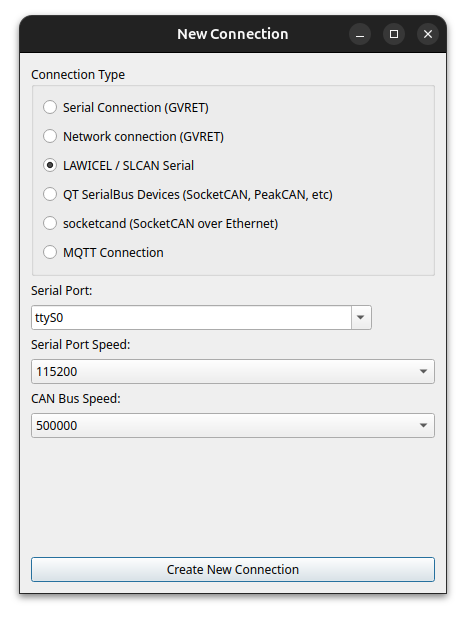
\includegraphics[width=0.8\textwidth]{Images/Savvy.png}
		\vspace{0.2cm}
		
		% La nota explicativa detallada va debajo, alineada a la izquierda
		\begin{flushleft}
			\footnotesize \textit{Nota.} Configuración de la conexión en SavvyCAN mediante el protocolo SLCAN, utilizando un ESP32 como puente serial hacia el bus CAN.
		\end{flushleft}
	\end{figure}
	
	\item Después de crear la conexión podremos notar como las tramas can se muestran en la pantalla como se ve en la Figura \ref{fig:imagencan}.
	
		\begin{figure}[H]
		\centering
		% El título y número se integran en el \caption (arriba de la imagen en APA)
		\caption{Conexion exitosa con el software SavvyCAN}
		\label{fig:imagencan}
		
		\vspace{0.3cm}
		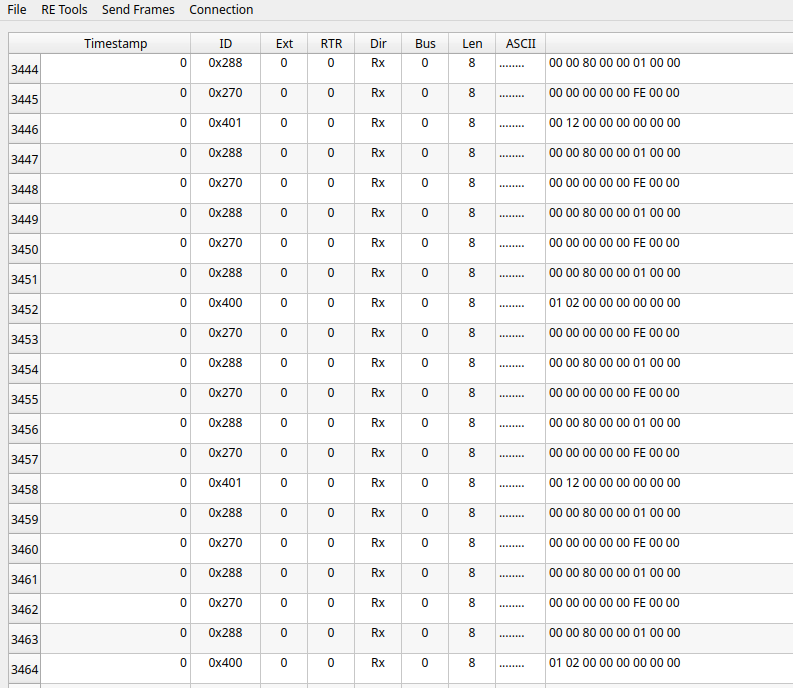
\includegraphics[width=1\textwidth]{Images/capturaCAN.png}
		\vspace{0.2cm}
		
		% La nota explicativa detallada va debajo, alineada a la izquierda
		\begin{flushleft}
			\footnotesize \textit{Nota.} Se detalla como los valores en hexadecimal están en cambio porque el vehículo al estar en contacto recibe muchas tramas CAN.
		\end{flushleft}
	\end{figure}
	
	\item Finalmente se demuestra exitosamente que si existen estas tramas CAN y en la siguiente parte veremos sus análisis y compresión del mismo.
	
\end{itemize}

\subsection{Análisis de tramas capturadas}
% Presentar capturas reales de SavvyCAN.
% Tabla con IDs CAN observados, periodicidad y longitud.
% Figura: screenshot de SavvyCAN con tramas reales.

Una vez establecida la comunicación con el vehículo (cuya arquitectura puede compararse con la de un sistema robótico compuesto por múltiples subsistemas interconectados), se procedió a la captura de tramas del bus de datos.

Como se observa en la Figura \ref{fig:imagencan}, los valores 
obtenidos en bruto no resultan interpretables de forma directa, por lo 
que es necesario aplicar ingeniería inversa para descifrar el significado 
de cada parámetro. Con base en los PIDs normalizados presentados en la 
Tabla \ref{tab:PID}, se identificaron en primera instancia aquellos 
parámetros conocidos como punto de partida para el análisis.

\subsubsection{Identificación de IDs}
% ID 0x7DF (broadcast), 0x7E8 (respuesta ECU principal).
% Diferencia entre tramas de diagnóstico y tramas nativas.
Para este análisis, se utilizó la herramienta Sniffer integrada en SavvyCAN, la cual permite monitorear e identificar en tiempo real las variaciones en los datos del bus. Un ejemplo práctico de su aplicación consiste en la conmutación de las luces altas del vehículo. Como se observa en la Figura \ref{fig:Sniffer}, la interfaz resalta dinámicamente los cambios en los bytes: los valores decrecientes se tiñen de color rojo, mientras que aquellos que se incrementan se muestran en verde, facilitando así la detección visual de las transiciones de datos.

\begin{figure}[htbp]
	\centering
	% 1. Forzamos el contador manual para que \ref{fig:Sniffer} extraiga el número exacto
	\refstepcounter{figure}
	\label{fig:Sniffer}
	
	% 2. Estructura de Título APA 7 (Alineado a la izquierda)
	\begin{flushleft}
		\bfseries Figura \thefigure \\
		\normalfont\itshape Interfaz de la herramienta Sniffer en SavvyCAN para el monitoreo del bus
	\end{flushleft}
	\vspace{2mm} % Espacio entre el título y la imagen
	
	% 3. Inserción de la Imagen (Cambia 'tu_imagen_sniffer' por el nombre de tu archivo)
	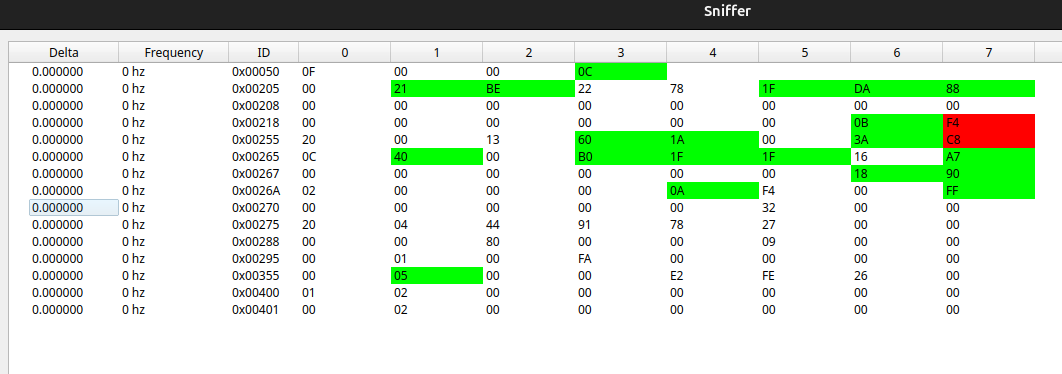
\includegraphics[width=1.0\textwidth]{Images/Sniffer.png} 
	
	\vspace{2mm} % Espacio entre la imagen y la nota
	
	% 4. Nota de Figura APA 7 (Alineada a la izquierda y en tamaño pequeño)
	\begin{flushleft}
		\itshape Nota. \normalfont Monitoreo pasivo en tiempo real de los identificadores de CAN (CAN IDs). La interfaz destaca dinámicamente las variaciones de los bytes empleando un código de colores: verde para incrementos en los valores y rojo para decrementos.
	\end{flushleft}
\end{figure}

Este procedimiento es fundamental para el proceso de ingeniería inversa; por ejemplo, al activar las luces de parqueo, se examinan las modificaciones en el Sniffer con el objetivo de aislar e identificar el identificador de CAN (CAN ID) y la trama hexadecimal específica que comanda dicha función.

Posteriormente, se analizó el comportamiento de las revoluciones por minuto (RPM) del motor en SavvyCAN. Aunque el estándar OBD-II define conceptualmente el PID 0x0C para solicitar de forma activa las RPM (como se listó en la Tabla A1 del Apéndice A), mediante el escaneo pasivo (Sniffer) se identificó que el vehículo transmite de forma autónoma estos datos bajo el CAN ID como muestra su estructura en la Figura \ref{fig:CAN_Frame}. Para validar este hallazgo, se capturaron las tramas en tiempo real bajo diferentes regímenes de operación (ver Figura \ref{fig:RPM_SNIFFER}).

\begin{figure}[htbp]
	\centering
	% 1. Forzamos el contador manual para que \ref{fig:RPM_SNIFFER} extraiga el número exacto
	\refstepcounter{figure}
	\label{fig:RPM_SNIFFER}
	
	% 2. Estructura de Título APA 7 (Alineado a la izquierda)
	\begin{flushleft}
		\bfseries Figura \thefigure \\
		\normalfont\itshape Monitoreo del bus CAN a un régimen constante de 2000 RPM
	\end{flushleft}
	\vspace{2mm} % Espacio entre el título y la imagen
	
	% 3. Inserción de la Imagen (Cambia 'tu_imagen_rpm_2000' por tu archivo correspondiente)
	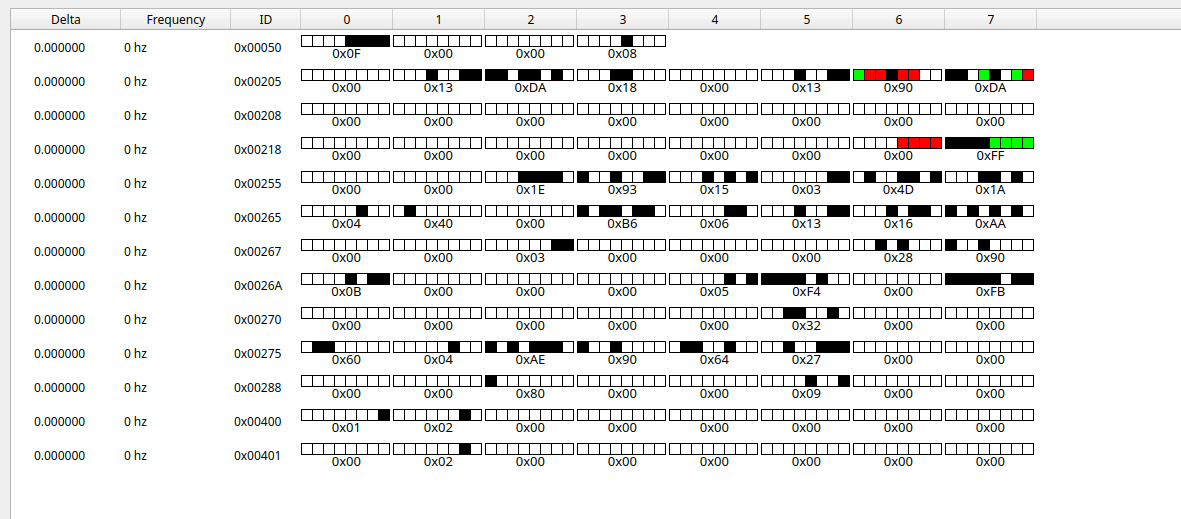
\includegraphics[width=1.0\textwidth]{Images/rpm_sniffer.png} 
	
	\vspace{2mm} % Espacio entre la imagen y la nota
	
	% 4. Nota de Figura APA 7 (Alineada a la izquierda y en tamaño pequeño)
	\begin{flushleft}
		\itshape Nota. \normalfont Captura de datos en el software SavvyCAN con el motor retenido a 2000 RPM. Las variaciones cromáticas en los bytes del ID \texttt{0x00255} permiten aislar las señales dinámicas vinculadas a la velocidad angular del cigüeñal del motor frente al estado de ralentí.
	\end{flushleft}
\end{figure}

Utilizando los datos crudos extraídos en un instante específico de la captura, se aplicaron las ecuaciones de ingeniería inversa correspondientes para decodificar los bytes y comparar el resultado matemático con el valor reflejado simultáneamente en el tacómetro del tablero de instrumentos del vehículo.

La ecuación matemática estándar que rige esta conversión, considerando la resolución universal de $0{,}25\,\text{RPM}/\text{bit}$ (factor de división por 4), se define en la Ecuación~\ref{eq:rpm_standard}:

\begin{equation}
	\text{RPM} = \frac{(\text{MSB} \times 256) + \text{LSB}}{4}
	\label{eq:rpm_standard}
\end{equation}

Donde $\text{MSB}$ representa el Byte Más Significativo (\textit{Byte Alto}) y $\text{LSB}$ representa el Byte Menos Significativo (\textit{Byte Bajo}).

\subsubsection{Candidato 1: ID \texttt{0x00255} (Bytes 2 y 3)}
A partir de la captura en vivo con el motor retenido, los bytes en estado activo para este ID presentaron los valores hexadecimales $\text{Byte}_2 = 1\text{E}_{16}$ y $\text{Byte}_3 = 93_{16}$. Convirtiendo dichos valores a base decimal se obtiene:
\begin{itemize}
	\item $\text{MSB} = 1\text{E}_{16} = (1 \times 16^1) + (14 \times 16^0) = 30$
	\item $\text{LSB} = 93_{16} = (9 \times 16^1) + (3 \times 16^0) = 147$
\end{itemize}

Sustituyendo estos valores en la ecuación de ingeniería inversa:
\begin{equation}
	\text{RPM}_{0255} = \frac{(30 \times 256) + 147}{4} = \frac{7680 + 147}{4} = \frac{7827}{4} = \mathbf{1956{,}75\,\text{RPM}}
\end{equation}

\subsubsection{Candidato 2: ID \texttt{0x00218} (Bytes 6 y 7)}
Este ID mostró alta volatilidad durante la aceleración. Evaluando sus bytes finales, cuyos valores registrados fueron $\text{Byte}_6 = 00_{16}$ y $\text{Byte}_7 = \text{FF}_{16}$, se procede con la conversión decimal:
\begin{itemize}
	\item $\text{MSB} = 00_{16} = 0$
	\item $\text{LSB} = \text{FF}_{16} = 255$
\end{itemize}

Sustituyendo en la ecuación fundamental:
\begin{equation}
	\text{RPM}_{0218} = \frac{(0 \times 256) + 255}{4} = \frac{255}{4} = \mathbf{63{,}75\,\text{RPM}}
\end{equation}

\subsubsection{Candidato 3: ID \texttt{0x00275} (Bytes 1 y 2)}
Este identificador, vinculado tentativamente a la posición del acelerador, marcó variaciones lineales leves. Tomando sus primeros bytes modificados, $\text{Byte}_1 = 00_{16}$ y $\text{Byte}_2 = \text{AE}_{16}$, se calcula su equivalente decimal:
\begin{itemize}
	\item $\text{MSB} = 00_{16} = 0$
	\item $\text{LSB} = \text{AE}_{16} = (10 \times 16^1) + (14 \times 16^0) = 174$
\end{itemize}

Sustituyendo en la ecuación:
\begin{equation}
	\text{RPM}_{0275} = \frac{(0 \times 256) + 174}{4} = \frac{174}{4} = \mathbf{43{,}50\,\text{RPM}}
\end{equation}

\subsubsection{Comparación de Resultados y Validación}

En la Tabla~\ref{tab:comparativa_ids} se organizan los datos calculados frente al valor real de referencia observado en el tacómetro analógico del vehículo ($2000\,\text{RPM}$).

\begin{table}[htbp]
	\centering
	\captionsetup{labelformat=simple, labelsep=newline, textfont=it, labelfont=bf}
	\caption{Comparativa de IDs candidatos para la determinación de la variable de RPM}
	\label{tab:comparativa_ids}
	% Definimos anchos fijos (p) que suman 14.0cm en total para una distribución perfecta en la hoja
	\begin{tabular}{p{1.8cm} p{2.5cm} p{2.8cm} p{3.8cm} p{3.1cm}}
		\toprule
		\rowcolor[rgb]{0.851, 0.851, 0.851}
		\textbf{CAN ID} & \textbf{Datos Hexadecimales} & \textbf{Valor Calculado} & \textbf{Desviación Absoluta} & \textbf{¿Es el ID de RPM?} \\
		\midrule
		\texttt{0x00255} & \texttt{0x1E 0x93} & \textbf{1956{,}75 RPM} & \textbf{43{,}25 RPM (2.1\%)} & \textbf{SÍ (Confirmado)} \\
		\texttt{0x00218} & \texttt{0x00 0xFF} & 63{,}75 RPM            & 1936{,}25 RPM                & NO \\
		\texttt{0x00275} & \texttt{0x00 0xAE} & 43{,}50 RPM            & 1956{,}50 RPM                & NO \\ 
		\bottomrule
	\end{tabular}
	\vspace{0.2cm}
	\begin{flushleft}
		\small
		\begin{center}
			\textit{Nota.} Comparativa de los identificadores del bus CAN analizados bajo un régimen constante de operación frente al valor nominal del tacómetro. Elaboración propia.
		\end{center}
	\end{flushleft}
\end{table}

A partir del análisis comparativo, se determina que el identificador del bus CAN perteneciente a las revoluciones por minuto es contundentemente el \textbf{ID \texttt{0x00255}}. 

La resolución matemática arroja un valor de $1956{,}75\,\text{RPM}$, lo cual representa una precisión del $97{,}9\%$ respecto al valor objetivo visualizado en el tablero de instrumentos.

El margen de desviación residual ($\approx 2{,}1\%$) no manifiesta un error en el modelado de la ecuación, sino que responde al comportamiento dinámico real del motor de combustión interna, cuyas micro-oscilaciones son captadas de forma pura por el bus de datos en milisegundos, mientras que la aguja física del cuadro de instrumentos actúa como un filtro mecánico amortiguado que suaviza la lectura visual para el conductor.

Los resultados demuestran que, mediante el análisis por ingeniería inversa de los identificadores (IDs) provistos por la herramienta SavvyCAN, es posible aislar e interpretar la estructura de las tramas CAN del vehículo.

\subsection{Selección final de PIDs para monitoreo de consumo}
% Justificar por qué se eligieron los 12 PIDs de la Tabla~\ref{tab:pids}.
% Tabla comparativa: PID disponible en Changan Honor vs Nissan Vanette.
% Criterio de conmutación MAF → Speed-Density si 0x10 no responde.
A continuación, se abordará la consulta de Identificadores de Parámetro (PIDs). A diferencia de los identificadores de trama (IDs) del bus CAN, que definen pasivamente la procedencia o prioridad de un mensaje, los PIDs constituyen peticiones activas enviadas hacia la Unidad de Control Electrónico (ECU), la cual procesa la solicitud y devuelve la información bajo un esquema de pregunta-respuesta. Este mecanismo interactivo representa el principio operativo fundamental de la mayoría de los escáneres automotrices comerciales. Con el propósito de determinar qué variables de telemetría están disponibles en el vehículo de prueba, se desarrolló inicialmente un algoritmo general diseñado para explorar y decodificar el mapa de bits de los PIDs soportados.

El código fuente en C++ presentado en la Figura \ref{fig:codigo_scanner_obd2} implementa la inicialización, inyección y lectura de datos sobre el bus CAN del vehículo. Este algoritmo configura el periférico nativo TWAI \citep{espressif_esp32_datasheet} a un régimen de 500 kbps para garantizar la sincronización temporal con la red automotriz a través del transceptor físico \citep{sn65hvd230_datasheet}. 

El procesamiento de datos se sintetiza en tres etapas operativas esenciales:
\begin{itemize}
	\item \textbf{Inicialización:} En la rutina \texttt{setup()}, se asignan los pines de control (GPIO 4 y 5) y se establece un filtro de aceptación total para habilitar la escucha completa del tráfico en el bus.
	\item \textbf{Transmisión Funcional:} La función \texttt{solicitarPIDsSoportados()} inyecta una trama de diagnóstico única (\textit{Single Frame}) bajo el identificador estándar \texttt{0x7DF} conforme a la norma ISO 15765-4 \citep{iso15765}. La solicitud invoca al Servicio 01 y al PID \texttt{0x00}, rellenando los bytes restantes con ceros (\textit{padding}) para mantener la simetría obligatoria de 8 bytes.
	\item \textbf{Filtrado Lógico:} En el bucle principal \texttt{loop()}, el sistema evalúa las tramas entrantes en el búfer. El algoritmo descarta el tráfico secundario y aísla exclusivamente las respuestas de la ECU de motor (\texttt{0x7E8}) que validen el servicio (\texttt{0x41 0x00}), extrayendo finalmente los 4 bytes del mapa de bits.
\end{itemize}

\begin{figure}[H]
	\caption{Algoritmo en C++ para la detección activa y decodificación del mapa de bits de PIDs soportados en el bus CAN.}
	\label{fig:codigo_scanner_obd2}
	
	\begin{lstlisting}[
		language=C++,
		basicstyle=\fontsize{9.5}{9}\ttfamily,
		columns=flexible,
		breaklines=true,
		breakatwhitespace=false,
		postbreak=\mbox{\textcolor{gray}{$\hookrightarrow$}\space}
		]
#include "driver/twai.h"
#define CAN_TX_PIN GPIO_NUM_5
#define CAN_RX_PIN GPIO_NUM_4

void setup() {
	Serial.begin(115200);
	while(!Serial);
	Serial.println("Iniciando Escaner de PIDs OBD-II...");
	twai_general_config_t g_config = TWAI_GENERAL_CONFIG_DEFAULT(CAN_TX_PIN, CAN_RX_PIN, TWAI_MODE_NORMAL);
	twai_timing_config_t t_config = TWAI_TIMING_CONFIG_500KBITS(); 
	twai_filter_config_t f_config = TWAI_FILTER_CONFIG_ACCEPT_ALL();
	if (twai_driver_install(&g_config, &t_config, &f_config) == ESP_OK) {
		Serial.println("Driver TWAI instalado con exito.");
	} else {
		while (1);
	}
	if (twai_start() == ESP_OK) {
		Serial.println("Driver TWAI iniciado.");
	} else {
		while (1);
	}
	delay(2000);
	solicitarPIDsSoportados();
}
void loop() {
	twai_message_t rx_msg;
	if (twai_receive(&rx_msg, pdMS_TO_TICKS(1000)) == ESP_OK) {
		// Filtrar respuestas OBD2 estandar (0x7E8) y Servicio 01
		if (rx_msg.identifier == 0x7E8 && rx_msg.data[1] == 0x41 && rx_msg.data[2] == 0x00) {
			Serial.print("Respuesta Recibida de la ECU ID: 0x");
			Serial.println(rx_msg.identifier, HEX);
			Serial.print("Mapa de bits de PIDs (Hex): ");
			for(int i = 3; i < 7; i++) {
				if(rx_msg.data[i] < 0x10) Serial.print("0");
				Serial.print(rx_msg.data[i], HEX);
				Serial.print(" ");
			}
			Serial.println("\n-----------------------------------------");}}
}
void solicitarPIDsSoportados() {
	twai_message_t tx_msg;
	tx_msg.identifier = 0x7DF; 
	tx_msg.extd = 0;           
	tx_msg.data_length_code = 8;
	tx_msg.data[0] = 0x02;     
	tx_msg.data[1] = 0x01;     
	tx_msg.data[2] = 0x00;     
	for(int i=3; i<8; i++) tx_msg.data[i] = 0x00; 	
	if (twai_transmit(&tx_msg, pdMS_TO_TICKS(1000)) == ESP_OK) {
		Serial.println("Solicitud PID 0x00 enviada correctamente.");
	}}		
	\end{lstlisting}
	
	\vspace{-3mm} % Ajuste de espaciado estándar para la nota	
	\small
	\textit{Nota.} Algoritmo estructurado para la inicialización y el control del periférico de comunicación automotriz mediante la inyección activa de tramas de diagnóstico funcional (ID \texttt{0x7DF}). Desarrollado a partir de las especificaciones de bajo nivel para el manejo del buffer y sincronización de bits con referencias de \citep{espressif_twai} y \citep{sae_j1979_2014}.
\end{figure}


% ==========================================
% SECCIÓN 3: RESULTADOS EN MONITOR SERIE
% ==========================================
\subsubsection{Resultados Obtenidos}
Tras compilar el código y conectar el sistema al puerto OBD-II del Changan Honor con el contacto en posición \textit{ON}, el monitor serie arrojó la siguiente salida a $115200\text{ baudios}$ ver Figura \ref{fig:monitor_serie_obd2}:

\begin{figure}[H]
	\caption{Captura de pantalla del monitor serie durante la ejecución del escáner de PIDs OBD-II (Changan Honor).}
	\label{fig:monitor_serie_obd2}
	\centering
	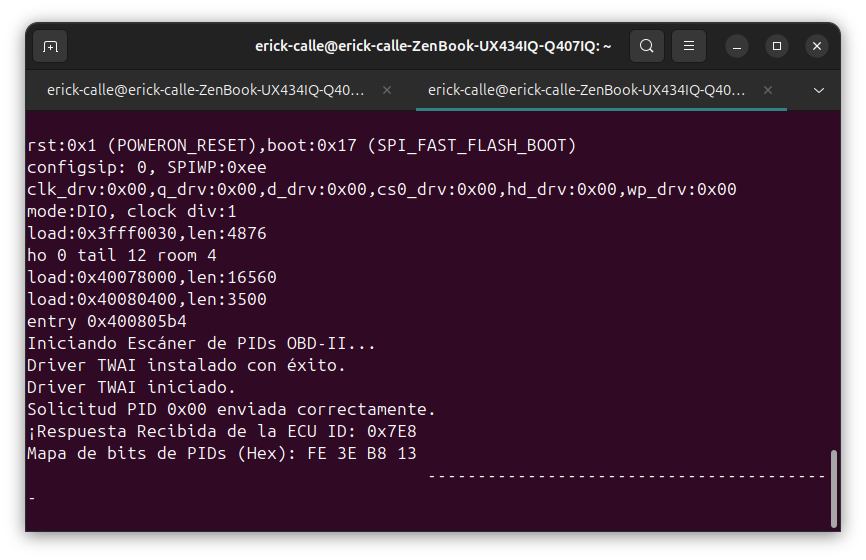
\includegraphics[width=0.85\textwidth]{Images/Serial.png} % Reemplaza por el nombre de tu archivo de imagen
	
	\vspace{2mm} % Ajuste de espaciado para la nota bajo formato APA
	\textit{Nota.} Registro de depuración en tiempo real, tomado sobre el Changan Honor, que muestra la inicialización correcta del controlador TWAI, el envío de la solicitud funcional (PID 0x00) y la respuesta hexadecimal (\texttt{FE 3E B8 13}) emitida por la unidad de control del motor (ECU).

\end{figure}

% ==========================================
% SECCIÓN 4: INTERPRETACIÓN DE RESULTADOS
% ==========================================
\subsubsection{Interpretación de Resultados}

La respuesta del bus CAN indica que la comunicación bidireccional fue exitosa. El identificador \texttt{0x7E8} confirma, bajo la arquitectura de segmentación de IDs de diagnóstico físico \cite{iso15765}, que la trama proviene directamente del módulo de control del motor (ECM).

Para determinar la disponibilidad de los comandos, el mapa de bits devuelto en formato hexadecimal, \texttt{FE 3E B8 13}, debe ser descompuesto en su representación binaria de 32 bits. Siguiendo el estándar SAE J1979 \citep{sae_j1979_2014}, cada bit se evalúa de izquierda a derecha (desde el bit más significativo hasta el menos significativo), donde un estado lógico de 1 indica que el PID está soportado por la ECU, y un estado de 0 indica su ausencia.

A continuación, se detalla la conversión de los cuatro bytes y el mapeo completo de los bits correspondientes al primer bloque de diagnóstico (PIDs del 0x01 al 0x20):
\begin{itemize}
	\item \textbf{Byte 1 (\texttt{FE}):} \texttt{1111 1110} $\rightarrow$ Soportados PIDs del 0x01 al 0x07; el PID 0x08 está ausente.
	\item \textbf{Byte 2 (\texttt{3E}):} \texttt{0011 1110} $\rightarrow$ Ausentes PIDs 0x09 y 0x0A; soportados del 0x0B al 0x0F; el PID 0x10 está ausente.
	\item \textbf{Byte 3 (\texttt{B8}):} \texttt{1011 1000} $\rightarrow$ Soportados PIDs 0x11, 0x13, 0x14 y 0x15; los demás están ausentes.
	\item \textbf{Byte 4 (\texttt{13}):} \texttt{0001 0011} $\rightarrow$ Soportados PIDs 0x1C, 0x1F y 0x20; los demás están ausentes.
\end{itemize}

La Tabla~\ref{tab:mapeo_pids_binario} describe la función específica y el impacto analítico de las variables críticas recuperadas en este mapa de bits para la caracterización dinámica del tren motriz.

\begin{table}[htbp]
	\centering
	\captionsetup{labelformat=simple, labelsep=newline, textfont=it, labelfont=bf}
	\caption{Mapeo binario de la respuesta hexadecimal FE 3E B8 13 y descripción de PIDs}
	\label{tab:mapeo_pids_binario}
	\small
	\renewcommand{\arraystretch}{1.3}
	% Definimos anchos fijos (p) que suman 14.2cm para mantener simetría exacta con tus otras tablas
	\begin{tabular}{p{1.5cm} p{1.2cm} p{2.2cm} p{3.0cm} p{6.3cm}}
		\toprule
		\rowcolor[rgb]{0.851, 0.851, 0.851}
		\textbf{Byte} & \textbf{Hex} & \textbf{Binario} & \textbf{PID Asociado} & \textbf{Descripción Técnica Resumida} \\
		
		Byte 1 & \texttt{FE} & \texttt{1111111\textbf{0}} & PID 0x01 - 0x08 & Estado de monitores y códigos de falla (DTC). \\
		&             &                            & \textbf{PID 0x0B (1)} & \textbf{MAP:} Presión del múltiple de admisión; clave para la densidad del aire. \\
		&             &                            & \textbf{PID 0x0C (1)} & \textbf{RPM:} Régimen de giro del motor y ciclos de llenado. \\ 
		
		Byte 2 & \texttt{3E} & \texttt{00\textbf{111110}} & \textbf{PID 0x0D (1)} & \textbf{VSS:} Velocidad del vehículo; convierte el consumo a L/km. \\
		&             &                            & \textbf{PID 0x0F (1)} & \textbf{IAT:} Temperatura de admisión; corrige la densidad por factor térmico. \\
		&             &                            & \texttt{PID 0x10 (0)} & \textbf{MAF:} Sensor de flujo de masa de aire (Ausente). \\ 
		
		Byte 3 & \texttt{B8} & \texttt{10111000}          & PID 0x11 - 0x18       & Posición del acelerador y sensores de oxígeno activos. \\ 
		
		Byte 4 & \texttt{13} & \texttt{00010011}          & PID 0x19 - 0x20       & Tiempo de operación y habilitación del bloque 0x21-0x40. \\
		\bottomrule
	\end{tabular}
	\vspace{0.2cm}
	\begin{flushleft}
		\small
		\begin{center}
			\textit{Nota.} El bit final del Byte 4 (\texttt{PID 0x20 = 1}) confirma que la ECU admite la consulta del siguiente rango de parámetros (PIDs 0x21 a 0x40) para expandir la adquisición de datos.
		\end{center}
	\end{flushleft}
\end{table}

% ==========================================
% SECCIÓN 5: CONCLUSIÓN DE LA PRUEBA
% ==========================================
\subsubsection{Conclusión de la prueba}

La ausencia absoluta del sensor MAF (\texttt{PID 0x10 = 0}), combinada con la disponibilidad simultánea y mandatoria de los sensores MAP, RPM e IAT, revela un aspecto fundamental de la arquitectura de la ECU: el sistema de inyección electrónica del vehículo no mide el flujo de aire de forma masiva directa, sino que calcula el caudal utilizando el método indirecto de Densidad de Velocidad (\textit{Speed Density}).

Este hallazgo define y valida el desarrollo matemático del sistema embebido. Al no contar con el PID 0x10, el microcontrolador deberá ser programado para resolver la ecuación de estado de los gases ideales combinada con la eficiencia volumétrica del motor en tiempo real. Al disponer de los datos de presión (MAP), temperatura (IAT) y velocidad angular (RPM), se confirma que el hardware desarrollado tiene acceso a todas las variables de estado requeridas para modelar el flujo de aire y estimar el consumo instantáneo de combustible de manera matemática y precisa.

El mismo procedimiento de escaneo se repitió sobre el segundo vehículo de prueba (Nissan Vanette), confirmando además que este sí soporta el PID 0x10 (MAF), tal como se resume en la Tabla~\ref{tab:pids_verificacion} del Capítulo~4. El listado completo y decodificado de los PIDs soportados por ambos vehículos se presenta en el Apéndice~O.
% ────────────────────────────────────────────────────────────
\section{Selección y justificación de componentes}
% Tu sección actual, sin cambios de fondo.
% Evalúa opciones → justifica → tabla resumen de componentes.
En esta sección se describen los componentes seleccionados para el sistema, priorizando su disponibilidad local en la ciudad de La Paz y su alineación con los objetivos del proyecto. La elección se basa en criterios de compatibilidad eléctrica, facilidad de integración, costo y rendimiento, con énfasis en soluciones robustas y accesibles.

\subsection{Interfaz OBD-II y controlador CAN}
% Conector, TJA1050 vs SN65HVD230, MCP2515.
Para leer datos del puerto OBD-II del vehículo, se requiere una conexión estable al bus CAN (Controller Area Network). Los componentes clave son:

\begin{enumerate}
	\item \textbf{Conector OBD-II}: Se utiliza un conector extraído de un escáner defectuoso para garantizar fiabilidad. Alternativamente, dos cables directos a las líneas CANH y CANL podrían emplearse, pero presentan riesgos de falsos contactos o conexiones inestables.Este posteriormente sera remplazado para una versión final del sistema.
	
	\item \textbf{Transceptores CAN}: Para convertir las señales diferenciales CANH/CANL en líneas digitales RX/TX compatibles con el microcontrolador, se evaluaron dos opciones:
	\begin{itemize}
		\item TJA1050 : Actúa como transceptor bidireccional, convirtiendo señales eléctricas del bus CAN en RX/TX como muestra en la Tabla B1 del Apéndice B. Es de bajo costo y disponible. Y su rango de voltajes de señal nos da el primer obstáculo como se ve en la Tabla B2 del Apéndice B al no ser de rango 3{,}3~V.
		
		\item SN65HVD230 (ver Apéndice C): Similar al anterior, pero optimizado para 3{,}3\,V; ideal, entonces, para microcontroladores de bajo voltaje.
		
	\end{itemize}
	Se seleccionó el SN65HVD230 por su stock local, popularidad en aplicaciones automotrices y compatibilidad con 3{,}3~V.
	
	\item \textbf{Controlador CAN (Periférico TWAI)}: Se seleccionó el ESP32 como unidad central debido a que integra periféricamente un controlador CAN a nivel de silicio, una característica ausente en la mayoría de microcontroladores convencionales de desarrollo ver Apéndice D. Este módulo nativo asume de forma autónoma la gestión de la capa de enlace de datos: empaqueta el payload, ejecuta el filtrado de mensajes por hardware para no saturar la CPU y administra la corrección de errores. 
\end{enumerate}

A todo esto se descartó el uso del escáner ELM327 de código abierto por su mayor costo y dependencia de conectividad inalámbrica (Bluetooth/Wi-Fi), que requeriría un ESP32 o Raspberry Pi con Python/MicroPython, complicando la integración.

\subsection{Microcontrolador del Sistema}
A diferencia de los esquemas de procesamiento distribuido, el núcleo de este sistema centraliza la adquisición de datos, el modelado matemático y la conectividad inalámbrica en un único circuito integrado, optimizando el espacio físico y suprimiendo la latencia de comunicación inter-procesador:

\begin{itemize}
	\item \textbf{ESP32}: Seleccionado como la unidad central de control debido a su arquitectura de alto rendimiento y su versatilidad periférica. El dispositivo asume de forma nativa dos funciones críticas para el proyecto: la gestión del bus CAN automotriz mediante su controlador interno TWAI (\textit{Two-Wire Automotive Interface}) y la transmisión inalámbrica de la telemetría hacia el servidor local a través de su pila de protocolos Wi-Fi integrada. 
\end{itemize}

\subsection{Periféricos de visualización}
% LCD 20×4 con módulo I2C vs OLED. Selección y justificación.
Se evaluaron varias pantallas para mostrar datos en tiempo real, priorizando tamaño, facilidad de conexión (I$^2$C o paralelo) y legibilidad para conductores:

\begin{itemize}

	\item \textbf{Pantalla LCD 20x4 o 16x2 }: Ofrece el tamaño óptimo para datos vehiculares, mejorando la usabilidad sin sacrificar simplicidad.
	
	\item \textbf{Pantalla OLED}: Se selecciono esta por ser compacta, conexión I$^2$C simple y compatible con 3{,}3~V según el Apéndice E.
	
\end{itemize}

\subsection{Lenguaje de programación}

El lenguaje de programación seleccionado es C++, por ser mas optimo para su programación y flexibilidad en entornos embebidos.

Finalmente en la Tabla \ref{tab:componentes_seleccionados} se muestran los componentes seleccionados :

\begin{table}[H]
	\centering
	\captionsetup{labelformat=simple, labelsep=newline, textfont=it, labelfont=bf, justification=raggedright, singlelinecheck=false}
	\caption{Componentes seleccionados y justificación técnica del sistema unificado}
	\label{tab:componentes_seleccionados}
	\small
	\renewcommand{\arraystretch}{1.3}
	% Mantenemos tus anchos fijos calibrados (3.5cm + 3.2cm + 7.5cm = 14.2cm) para un ajuste perfecto
	\begin{tabular}{p{3.5cm} p{3.2cm} p{7.5cm}}
		\toprule
		\rowcolor[rgb]{0.851, 0.851, 0.851}
		\textbf{Componente} & \textbf{Selección} & \textbf{Ventajas y justificación en el proyecto} \\ 
		\midrule
		Interfaz OBD-II & Conector OBD-II estándar & Permite una conexión mecánica y eléctrica estable directamente con el puerto de diagnóstico del vehículo. \\
		
		Microcontrolador y Controlador CAN & ESP32 & Centraliza el procesamiento, el modelado matemático de consumo y la conectividad Wi-Fi. Su periférico nativo TWAI elimina la necesidad de chips controladores externos como el MCP2515. \\ 
		
		Transceptor CAN & SN65HVD230 & Opera nativamente a 3,3 V, acoplándose de forma segura a los pines del ESP32. Traduce las señales lógicas a los niveles diferenciales del bus CAN automotriz. \\ 
		
		Pantalla de visualización & OLED & Ofrece excelente legibilidad en entornos con alta iluminación solar y mejor adaptación a ser 3,3 V. \\
		
		Lenguaje de programación & C++ (Entorno Arduino) & Cuenta con librerías maduras y de bajo nivel para el manejo del periférico TWAI, optimizando el tiempo de desarrollo y la estabilidad del sistema embebido. \\
		\bottomrule
	\end{tabular}
	\vspace{0.2cm}
	\begin{flushleft}
		\small
		\begin{center}
			\textit{Nota.} Arquitectura de hardware optimizada y simplificada a partir de la centralización de procesos en un único núcleo de ejecución.
		\end{center}
	\end{flushleft}
\end{table}
% ────────────────────────────────────────────────────────────
\section{Diseño de hardware}

\subsection{Módulo de Interfaz CAN Bus (SN65HVD230 + ESP32)}

El transceptor SN65HVD230 de Texas Instruments fue seleccionado como interfaz física 
entre el microcontrolador ESP32 y el bus CAN del vehículo. A diferencia de soluciones 
basadas en el MCP2515, este transceptor no requiere controlador CAN externo ni 
comunicación SPI, dado que el ESP32 integra nativamente el periférico 
TWAI\textsuperscript{\textregistered} (\textit{Two-Wire Automotive Interface}), 
compatible con el estándar ISO 11898-1 (CAN 2.0B). La conexión entre ambos 
dispositivos se reduce a dos líneas lógicas: TX y RX entre el ESP32 y el 
transceptor, y dos líneas diferenciales CANH y CANL hacia el bus del vehículo.

\subsubsection{Configuración del Periférico TWAI\textsuperscript{\textregistered} del ESP32}

La velocidad del bus CAN automotriz opera típicamente a 500~kbps bajo el estándar 
ISO 11898-1. La configuración del periférico TWAI\textsuperscript{\textregistered} 
se realiza directamente mediante el driver oficial de Espressif en el framework 
ESP-IDF, sin necesidad de calcular registros de temporización manualmente. 
La inicialización del bus se estructura en tres parámetros fundamentales, 
tal como se muestra en la Figura \ref{fig:twai_init}:

\begin{figure}[H]
	\caption{Inicialización del periférico TWAI\textsuperscript{\textregistered} 
			del ESP32 a 500~kbps.}
	\label{fig:twai_init}
	\begin{lstlisting}[language=C++, basicstyle=\fontsize{10}{10}\ttfamily, breaklines=true]
twai_general_config_t g_config = 
TWAI_GENERAL_CONFIG_DEFAULT(GPIO_NUM_4, GPIO_NUM_5, TWAI_MODE_NORMAL);
twai_timing_config_t t_config = TWAI_TIMING_CONFIG_500KBITS();
twai_filter_config_t f_config = TWAI_FILTER_CONFIG_ACCEPT_ALL();
		
twai_driver_install(&g_config, &t_config, &f_config);
twai_start();
	\end{lstlisting}
	\vspace{-1mm}
	\noindent\small\textit{Nota.} La macro \texttt{TWAI\_TIMING\_CONFIG\_500KBITS()} 
	configura automáticamente los parámetros de bit-timing (TQ, PropSeg, PhaseSeg1, 
	PhaseSeg2 y SJW) para operar a 500~kbps sobre el reloj interno del ESP32 
	a 80~MHz, eliminando el cálculo manual de registros CNF.
\end{figure}

\subsubsection{Filtrado de Tramas CAN por Identificador}

El periférico TWAI\textsuperscript{\textregistered} incorpora un filtro de 
aceptación por hardware configurable mediante una máscara de 32 bits, equivalente 
funcional a los registros RXF y RXM del MCP2515. Para recibir únicamente la 
respuesta de la ECU principal en consultas OBD-II (ID \texttt{0x7E8}), se 
configura el filtro de la siguiente manera (ver Figura \ref{fig:twai_filter}):

\begin{figure}[H]
	\caption{Configuración del filtro de aceptación para recepción exclusiva 
			de respuestas OBD-II.}
	\label{fig:twai_filter}
	\begin{lstlisting}[language=C++, basicstyle=\fontsize{10}{10}\ttfamily, breaklines=true]
twai_filter_config_t f_config = {
	.acceptance_code = (0x7E8 << 21), // ID aceptado: respuesta ECU
	.acceptance_mask = ~(0x7FF << 21), // Mascara exacta de 11 bits
	.single_filter   = true
};
	\end{lstlisting}
	\vspace{-1mm}
	\noindent\small\textit{Nota.} El desplazamiento de 21 bits se debe al formato 
	interno del registro de filtro del TWAI\textsuperscript{\textregistered}, que 
	ubica el identificador de 11 bits en los bits más significativos de la palabra 
	de 32 bits. La máscara \texttt{0x7FF} garantiza coincidencia exacta del 
	identificador, descartando cualquier otra trama presente en el bus y reduciendo 
	la carga de procesamiento del sistema.
\end{figure}

\subsection{Módulo de Visualización (OLED I2C)}

Para la visualización local de parámetros se empleó una pantalla OLED de 
128$\times$64 píxeles controlada mediante el protocolo I2C, conectada 
directamente al ESP32. La dirección esclava del dispositivo es \texttt{0x3C}, 
configurable a \texttt{0x3D} mediante el puente de soldadura en la placa del 
módulo. La gestión del display se realizó mediante la biblioteca 
\texttt{Adafruit\_SSD1306}, que abstrae el protocolo de comunicación y provee 
funciones de renderizado de texto y gráficos primitivos.

\subsubsection{Distribución de la información en pantalla}

A diferencia de un esquema de múltiples pantallas navegables, el firmware mantiene una única pantalla fija que se redibuja por completo cada \texttt{OLED\_REFRESH\_PERIOD\_MS} (400~ms por defecto), priorizando en todo momento los datos que más se consultan al conducir: el consumo y el costo acumulado del viaje. La distribución de la información en esa pantalla se detalla en la Tabla \ref{tab:distribucion_pantallas}.

\begin{table}[H]
	\centering
	\captionsetup{labelformat=simple, labelsep=newline, textfont=it, labelfont=bf, justification=raggedright, singlelinecheck=false}
	\caption{Distribución de la información en la pantalla OLED}
	\label{tab:distribucion_pantallas}
	\small
	\renewcommand{\arraystretch}{1.3}
	% Mantenemos la calibración exacta de anchos fijos (3.0cm + 11.2cm = 14.2cm)
	\begin{tabular}{p{3.0cm} p{11.2cm}}
		\toprule
		\rowcolor[rgb]{0.851, 0.851, 0.851}
		\textbf{Zona} & \textbf{Contenido mostrado} \\
		\midrule
		Línea superior & RPM del motor (PID \texttt{0x0C}) y velocidad del vehículo (PID \texttt{0x0D}), en texto pequeño. \\

		Centro (texto grande) & Consumo instantáneo: L/100~km si el vehículo se mueve (velocidad $>2$~km/h), o L/h si está detenido o en ralentí, para no dividir entre una velocidad cercana a cero. \\

		Centro (texto grande) & Costo acumulado del viaje, en bolivianos, calculado a partir del combustible ya consumido (\texttt{trip\_fuel\_L} $\times$ \texttt{FUEL\_PRICE\_BS\_PER\_L}), no de la tasa instantánea. \\

		Línea inferior 1 & Distancia y combustible acumulados del viaje. \\

		Línea inferior 2 & Estado de la comunicación CAN (\texttt{CAN:OK}/\texttt{CAN:--}) y estado del panel web: dirección IP del punto de acceso si está activo, o \texttt{srv:--} en caso contrario. \\
		\bottomrule
	\end{tabular}
	\vspace{0.2cm}
	\begin{flushleft}
		\small
		\begin{center}
			\textit{Nota.} No hay navegación entre pantallas ni pulsador físico asociado a la OLED: toda la información relevante para conducir se muestra simultáneamente en esta única vista, y el detalle adicional (MAP, IAT, eficiencia volumétrica, flujo de aire y combustible calculados, etc.) queda disponible en el panel web y en el registro de la tarjeta microSD (Tabla~\ref{tab:estructura_csv}).
		\end{center}
	\end{flushleft}
\end{table}

\subsection{Módulo de Registro en Memoria (SSD)}

Para el almacenamiento persistente de los datos adquiridos se utilizó una 
memoria de estado sólido conectada al ESP32 mediante el protocolo SPI. 
Los registros se almacenan en formato CSV con marca de tiempo, permitiendo 
su posterior análisis en herramientas de ofimática o procesamiento de datos.
Cada sesión genera un archivo independiente identificado por número de 
sesión correlativo, preservando el historial completo de adquisiciones.

\subsubsection{Estructura del Archivo de Registro}

Cada fila del archivo CSV registra una muestra completa de los parámetros 
activos en ese instante, con la estructura definida en la Tabla \ref{tab:estructura_csv}.

\begin{table}[H]
	\centering
	\captionsetup{labelformat=simple, labelsep=newline, textfont=it, labelfont=bf, justification=raggedright, singlelinecheck=false}
	\caption{Estructura real del registro CSV escrito por \texttt{sdLoggerTask()} (\texttt{sd\_logger.cpp})}
	\label{tab:estructura_csv}
	\small
	\renewcommand{\arraystretch}{1.15}
	% Mantenemos la calibración exacta de anchos fijos (3.5cm + 2.0cm + 8.7cm = 14.2cm)
	\begin{tabular}{p{3.5cm} p{2.0cm} p{8.7cm}}
		\toprule
		\rowcolor[rgb]{0.851, 0.851, 0.851}
		\textbf{Campo} & \textbf{Tipo} & \textbf{Descripción} \\
		\midrule
		\texttt{uptime\_ms}       & uint32 & Tiempo transcurrido desde el arranque del sistema, en milisegundos (\texttt{millis()}). \\
		\texttt{rpm}              & uint16 & Revoluciones por minuto del motor (PID \texttt{0x0C}). \\
		\texttt{speed\_kmh}       & float  & Velocidad del vehículo, en km/h (PID \texttt{0x0D}). \\
		\texttt{map\_kpa}         & float  & Presión absoluta del colector de admisión, en kPa (PID \texttt{0x0B}). \\
		\texttt{iat\_c}           & float  & Temperatura del aire de admisión, en °C (PID \texttt{0x0F}). \\
		\texttt{coolant\_c}       & float  & Temperatura del líquido refrigerante del motor, en °C (PID \texttt{0x05}). \\
		\texttt{ve\_pct}          & float  & Eficiencia volumétrica interpolada de \texttt{kVeTable} para el régimen actual, en \%. \\
		\texttt{maf\_gs}          & float  & Flujo másico de aire estimado por el modelo Speed-Density, en g/s. \\
		\texttt{fuel\_gs}         & float  & Flujo másico de combustible calculado, en g/s. \\
		\texttt{instant\_Lh}      & float  & Consumo instantáneo en L/h (válido en ralentí o vehículo detenido). \\
		\texttt{instant\_L100km}  & float  & Consumo instantáneo en L/100~km (válido con el vehículo en movimiento). \\
		\texttt{trip\_km}         & float  & Distancia acumulada del viaje, en km. \\
		\texttt{trip\_fuel\_L}    & float  & Combustible acumulado del viaje, en L. \\
		\texttt{trip\_avg\_L100km} & float & Consumo promedio acumulado del viaje, en L/100~km. \\
		\texttt{can\_status}      & uint8  & Estado de la comunicación CAN (\texttt{0}=INIT, \texttt{1}=OK, \texttt{2}=SIN\_RESPUESTA, \texttt{3}=ERROR\_BUS, \texttt{4}=BUS\_OFF). \\
		\texttt{trip\_cost\_bs}   & float  & Costo acumulado del viaje, en bolivianos (\texttt{trip\_fuel\_L}~$\times$~\texttt{FUEL\_PRICE\_BS\_PER\_L}). \\
		\texttt{baro\_kpa}        & float  & Presión barométrica de referencia, en kPa (PID \texttt{0x33} real, o estimación del modelo ISA si no está soportado). \\
		\texttt{baro\_is\_estimated} & bool & \texttt{1} si \texttt{baro\_kpa} proviene de la estimación ISA; \texttt{0} si es una lectura real por PID \texttt{0x33}. \\
		\bottomrule
	\end{tabular}
	\vspace{0.2cm}
	\begin{flushleft}
		\small
		\begin{center}
			\textit{Nota.} Fila exacta escrita cada \texttt{SD\_LOG\_INTERVAL\_MS} (1000~ms por defecto) mientras hay una lectura CAN válida; el archivo se abre una sola vez por sesión y cada fila se escribe en modo \textit{append} con \texttt{flush()} inmediato, de forma que una pérdida de energía no descarta filas ya escritas. Los ajustes de combustible STFT/LTFT (PIDs \texttt{0x06}/\texttt{0x07}) se usan internamente para corregir el cálculo (Capítulo~3, lazo cerrado) pero no se registran como columnas propias de este CSV.
		\end{center}
	\end{flushleft}
\end{table}


\subsection{Módulo de Comunicación Inalámbrica y Servidor Web}

El mismo ESP32 que gestiona la adquisición CAN opera simultáneamente como 
punto de acceso WiFi (\textit{Access Point}), exponiendo un servidor web 
embebido para la visualización remota de parámetros en tiempo real desde 
cualquier dispositivo conectado a la red local generada. No se requiere 
conexión a internet ni infraestructura de red externa.

\subsubsection{Arquitectura del Servidor Web Embebido}

El servidor web se implementó con la biblioteca \texttt{ESPAsyncWebServer}, 
que permite atender peticiones HTTP y mantener conexiones WebSocket de forma 
asíncrona sin bloquear el bucle principal de adquisición CAN. La interfaz 
gráfica HTML/CSS/JS se almacena en la partición SPIFFS del ESP32 y se sirve 
estáticamente al cliente. La actualización de datos en tiempo real se realiza 
mediante WebSocket, evitando el \textit{polling} HTTP y reduciendo la latencia 
de visualización. El flujo de datos completo se ilustra en la 
Figura~\ref{fig:flujo_web}.

\begin{figure}[htbp]
	\centering
	% Título alineado a la izquierda estilo APA 7 idéntico a tus tablas
	\captionsetup{labelformat=simple, labelsep=newline, textfont=it, labelfont=bf, justification=raggedright, singlelinecheck=false}
	\caption{Flujo de datos desde el bus CAN hasta el cliente web}
	\label{fig:flujo_web}
	
	\begin{tikzpicture}[
		% Configuración de Estilos de los Bloques
		node_ext/.style={rectangle, draw=gray!70!black, fill=gray!5, thick, rounded corners=3pt, text width=5.2cm, align=center, minimum height=0.9cm, font=\small},
		node_core1/.style={rectangle, draw=blue!60!black, fill=blue!4, thick, rounded corners=3pt, text width=5.2cm, align=center, minimum height=0.9cm, font=\small},
		node_core0/.style={rectangle, draw=teal!60!black, fill=teal!4, thick, rounded corners=3pt, text width=5.2cm, align=center, minimum height=0.9cm, font=\small},
		node_hw/.style={rectangle, draw=gray!50, fill=gray!1, dashed, rounded corners=3pt, text width=3.4cm, align=center, minimum height=0.9cm, font=\small},
		arrow/.style={-{Stealth[scale=1.2]}, draw=black!70, thick}
		]
		
		% --- UBICACIÓN DE NODOS ---
		
		% Origen externo
		\node (can) [node_ext] {\textbf{Bus CAN (Vehículo)}};
		
		% Bloque del Núcleo 1 (Adquisición y Almacenamiento)
		\node (twai) [node_core1, below=0.8cm of can] {\textbf{ESP32 - Núcleo 1}\\Periférico TWAI\\(Adquisición CAN)};
		
		% Periféricos locales de salida (a los lados del Núcleo 1)
		\node (oled) [node_hw, left=0.7cm of twai] {\textbf{OLED I2C}\\(Visualización local)};
		\node (ssd) [node_hw, right=0.7cm of twai] {\textbf{SSD SPI}\\(Registro CSV persistente)};
		
		% Bloques del Núcleo 0 (Conectividad y Servidor Web)
		\node (ap) [node_core0, below=1.0cm of twai] {\textbf{ESP32 - Núcleo 0}\\Access Point WiFi\\(192.168.4.1)};
		
		\node (web) [node_core0, below=0.6cm of ap] {\textbf{ESPAsyncWebServer}\\HTTP $\rightarrow$ \texttt{index.html} (SPIFFS)};
		
		\node (ws) [node_core0, below=0.6cm of web] {\textbf{WebSocket}\\Transmisión de datos \texttt{JSON}};
		
		% Destino final (Entorno del cliente)
		\node (nav) [node_ext, below=1.0cm of ws] {\textbf{Navegador Cliente}\\(Renderizado en Laptop/Móvil)};
		
		\node (chart) [node_ext, below=0.6cm of nav] {\textbf{Canvas nativo}\\Gráficas en tiempo real};
		
		% --- CONEXIONES / FLECHAS ---
		
		\draw [arrow] (can) -- (twai);
		\draw [arrow] (twai) -- (oled);
		\draw [arrow] (twai) -- (ssd);
		
		% Enlace inter-núcleos
		\draw [arrow] (twai) -- (ap) node[midway, right, font=\scriptsize\itshape, text=black!60] {Memoria compartida};
		
		\draw [arrow] (ap) -- (web);
		\draw [arrow] (web) -- (ws);
		
		% Transmisión inalámbrica hacia el cliente
		\draw [arrow] (ws) -- (nav) node[midway, right, font=\scriptsize\itshape, text=black!60] {Enlace WiFi (WebSockets)};
		
		\draw [arrow] (nav) -- (chart);
		
	\end{tikzpicture}
	
	\vspace{0.2cm}
	\begin{flushleft}
		\small
		\begin{center}
			\textit{Nota.} Todos los módulos operan sobre el mismo microcontrolador ESP32, aprovechando el núcleo dual del procesador: el núcleo 0 gestiona la comunicación WiFi y el servidor web, mientras que el núcleo 1 ejecuta la adquisición CAN y la escritura en SSD.
		\end{center}
	\end{flushleft}
\end{figure}
\subsubsection{Formato de Trama JSON por WebSocket}

Cada 500~ms el ESP32 serializa los parámetros activos en un objeto JSON 
y lo transmite a todos los clientes conectados mediante difusión 
(\textit{broadcast}) WebSocket con la estructura en código como se muestra en la Figura \ref{fig:json_trama}:

\begin{figure}[H]
	\caption{Estructura de la trama JSON transmitida por WebSocket 
			al cliente web.}
	\label{fig:json_trama}
	\begin{lstlisting}[language=C++, basicstyle=\fontsize{10}{10}\ttfamily, breaklines=true]
// Serializacion en el ESP32
String buildJSON(OBDData& d) {
	return "{\"rpm\":"      + String(d.rpm, 0)       +
		",\"vel\":"      + String(d.velocidad)     +
		",\"temp\":"     + String(d.temp_ref)      +
		",\"carga\":"    + String(d.carga, 1)      +
		",\"maf\":"      + String(d.maf, 2)        +
		",\"stft\":"     + String(d.stft_b1, 1)    +
		",\"ltft\":"     + String(d.ltft_b1, 1)    +
		",\"ts\":"       + String(millis())        + "}";
}
		
// Envio broadcast a todos los clientes WebSocket
ws.textAll(buildJSON(currentData));
	\end{lstlisting}
	\vspace{-3mm}
	\noindent\small\textit{Nota.} El cliente web recibe el JSON y actualiza 
	las gráficas mediante Chart.js sin recargar la página, logrando una 
	visualización fluida con latencia inferior a 100~ms en condiciones normales 
	de red local.
\end{figure}

\subsection{Diagrama esquemático general}
% Tu contenido actual: 4 bloques funcionales con figuras.
En esta sección se presentará el diseño esquemático del sistema, realizando el cálculo y selección de los valores óptimos para cada componente con base en las recomendaciones de sus respectivas hojas de datos. Para facilitar el análisis y diseño, el sistema se ha dividido en los siguientes subsistemas:

\begin{itemize}
	
	\item \textbf{Sistema de alimentación:} En este subsistema se incorporarán las etapas de protección, regulación y filtrado de energía. Su principal objetivo es garantizar una alimentación estable y segura para todos los componentes del sistema, minimizando los efectos de ruido eléctrico, interferencias y transitorios de tensión.
	
	\item \textbf{Sistema transceptor CAN:} Se analizará el funcionamiento del transceptor CAN SN65HVD230, implementando una configuración optimizada que permita reducir el espacio ocupado en la PCB y mantener una comunicación confiable con la red CAN del vehículo.
	
	\item \textbf{Sistema de procesamiento:} Comprende el microcontrolador ESP32 y todos los componentes necesarios para su correcto funcionamiento, incluyendo circuitos auxiliares, interfaces de comunicación y conexiones para los distintos periféricos del sistema.
	
	\item \textbf{Sistema de visualización:} Se desarrollará la interfaz de conexión hacia una pantalla externa ubicada en el tablero del vehículo, para que el usuario disponga de la información relevante.

	\item \textbf{Sistema de almacenamiento de datos:} Se implementará una interfaz para memoria microSD destinada al almacenamiento de los datos obtenidos por el sistema, de modo que puedan analizarse y procesarse más adelante.

	\item \textbf{Sistema de programación:} Incluye los componentes necesarios para la configuración, programación y actualización del firmware del ESP32; con esto se simplifica el desarrollo y mantenimiento del dispositivo.
	
	\item \textbf{Sistema de monitoreo y estado:} Se incorporarán indicadores luminosos (LEDs) que permitirán visualizar el estado operativo del sistema y facilitar tareas de diagnóstico durante su funcionamiento.
	
\end{itemize}

Todos estos subsistemas han sido concebidos para su implementación en una placa de circuito impreso (PCB). A continuación, se desarrollan los esquemáticos correspondientes a cada uno de ellos.


\subsubsection{Sistema de alimentación}

Se contempla la obtención del voltaje de alimentación principal directamente desde el pin 16 del conector OBD-II del vehículo, el cual proporciona una tensión nominal de 12~V proveniente de la batería (ver Figura \ref{fig:pinobd}). Debido a que los circuitos electrónicos internos operan a tensiones significativamente menores, es indispensable implementar una etapa previa de acondicionamiento, protección y reducción de voltaje mediante un convertidor reductor (\textit{step-down}). 

Con el propósito de mitigar perturbaciones eléctricas severas comunes en el entorno automotriz, tales como transitorios de conmutación o picos de tensión, se diseñó una etapa de protección robusta previa a la regulación síncrona a niveles de 5~V y 3{,}3~V. El flujo lógico y secuencial planificado para esta etapa de potencia se detalla en la Figura \ref{fig:esquema_potencia}.

\begin{figure}[H]
	\centering
	% Formato APA 7 con alineación estricta a la izquierda y protección para el índice
	\captionsetup{labelformat=simple, labelsep=newline, textfont=it, labelfont=bf, justification=raggedright, singlelinecheck=false}
	\caption[Diagrama de bloques del sistema de protección y regulación de energía (12V a 3.3V)]{Diagrama de bloques del sistema de protección y regulación de energía}
	\label{fig:esquema_potencia}
	
	% Escalamos el diagrama automáticamente para que ocupe el ancho del texto
	\resizebox{\textwidth}{!}{%
		\begin{tikzpicture}[
			% Configuración de estilos visuales para las etapas
			etapa_in/.style={rectangle, draw=red!60!black, fill=red!5, thick, rounded corners=3pt, text width=2.4cm, align=center, minimum height=1.1cm, font=\small},
			etapa_prot/.style={rectangle, draw=gray!70!black, fill=gray!5, thick, rounded corners=3pt, text width=2.4cm, align=center, minimum height=1.1cm, font=\small},
			etapa_reg/.style={rectangle, draw=orange!70!black, fill=orange!5, thick, rounded corners=3pt, text width=2.4cm, align=center, minimum height=1.1cm, font=\small},
			etapa_out/.style={rectangle, draw=teal!70!black, fill=teal!4, thick, rounded corners=3pt, text width=2.4cm, align=center, minimum height=1.1cm, font=\small},
			arrow/.style={-{Stealth[scale=1.2]}, draw=black!70, thick}
			]
			
			% --- UBICACIÓN HORIZONTAL DE LOS BLOQUES ---
			\node (pin16) [etapa_in] {\textbf{Pin 16 (12V)}\\Entrada OBD-II};
			
			\node (fuse) [etapa_prot, right=0.5cm of pin16] {\textbf{Fusible}\\Protección contra sobrecorriente};
			
			\node (diode) [etapa_prot, right=0.5cm of fuse] {\textbf{Diodo TVS}\\Supresión de picos de voltaje};
			
			% Conexión directa del TVS al Buck de 3.3V
			\node (reg33v) [etapa_reg, right=0.5cm of diode] {\textbf{Regulador 5V}\\(TPS54302 Buck)};
			
			\node (esp32) [etapa_out, right=0.5cm of reg33v] {\textbf{ESP32}\\y Periféricos 3,3V};
			
			% --- CONEXIONES / FLECHAS ---
			\draw [arrow] (pin16) -- (fuse);
			\draw [arrow] (fuse) -- (diode);
			\draw [arrow] (diode) -- (reg33v) node[midway, below, font=\scriptsize\bfseries\color{black!60}] {12V};
			\draw [arrow] (reg33v) -- (esp32) node[midway, below, font=\scriptsize\bfseries\color{black!60}] {5V};
			
		\end{tikzpicture}%
	}
	
	\vspace{3mm}
	\small\raggedright
	\textit{Nota.} Topología de conversión directa de alta eficiencia basada en el regulador síncrono TPS54302. Esta configuración reduce directamente la tensión del bus automotriz de 12~V a 3{,}3~V nominales, optimizando la disipación térmica y garantizando un suministro eléctrico estable para el microcontrolador y sus periféricos críticos, previniendo caídas de tensión (\textit{brownouts}) bajo las exigencias de consumo del transmisor Wi-Fi \cite{espressif_esp32_datasheet}.
\end{figure}

Con base en el diagrama de bloques estructurado, se procedió a la selección rigurosa de los
componentes electrónicos para la etapa de potencia. Esta etapa es crítica para adaptar los 12~V
nominales provenientes del pin 16 del conector OBD-II a los niveles lógicos del sistema,
garantizando fiabilidad frente a las exigentes condiciones eléctricas del entorno automotriz:

\begin{enumerate}
	
	\item \textbf{Fusible rearmable (PTC):} Debido a que la red eléctrica del vehículo está
	expuesta a cortocircuitos y sobrecorrientes transitorias, se descartó el uso de fusibles
	tradicionales de un solo uso. Se optó por el fusible rearmable polimérico PTC modelo
	LUTE 1812L150/33GR, el cual soporta una tensión máxima de operación de 33~V, una corriente
	de mantenimiento (\textit{hold current}) de 1{,}5~A y una corriente de disparo
	(\textit{trip current}) de 3{,}0~A en encapsulado SMD 1812,datos que muestra la hoja de datos del componente en el Apendice F \citep{bourns_bsmd1812}. Su
	principal ventaja radica en su capacidad de restablecer automáticamente la conducción una
	vez que la falla desaparece y el componente se enfría, eliminando la necesidad de
	reemplazo físico en el campo.
	
	\item \textbf{Diodo Schottky de protección de polaridad inversa (D1):} Para evitar daños
	irreversibles ante una conexión accidental con polaridad invertida en el puerto OBD-II, se
	integró el diodo Schottky SS34 en serie con la línea de alimentación positiva. Según su
	hoja de datos mostrada en el Apéndice G , este componente soporta una tensión inversa repetitiva máxima
	($V_{RRM}$) de 40~V y una corriente media rectificada ($I_O$) de 3~A, con una caída de
	tensión directa típica de 550~mV a plena carga \citep{onsemi_ss36}. Su encapsulado
	DO-214AB (SMA) ofrece excelente disipación térmica en condiciones de alta corriente.
	
	\item \textbf{Diodo TVS (\textit{Transient Voltage Suppressor}):} Para suprimir el ruido
	electromagnético y proteger la circuitería contra picos de voltaje severos (tales como
	los transitorios de desconexión de carga, o \textit{load dump}, propios del entorno
	automotriz, que pueden superar los 40~V) se integró el diodo TVS unidireccional SMAJ18A
	en paralelo con la línea de alimentación, inmediatamente después del fusible PTC y el
	diodo de polaridad. De acuerdo con su hoja de datos (ver Apéndice H), su tensión de trabajo
	(\textit{stand-off voltage}) de 18~V permite la libre operación del voltaje nominal de
	la batería del vehículo, mientras que su tensión de sujeción máxima (\textit{clamping
		voltage}) de 29{,}2~V a una corriente de pico de 13{,}7~A \citep{vishay_smaj28a} garantiza
	que ningún transitorio destructivo alcance al regulador.  La potencia de disipación de pulso pico es de
	400~W con una forma de onda de 10/1000~µs, suficiente para absorber los transitorios
	definidos por la norma ISO 7637-2 en entornos automotrices.
	
	\item \textbf{Regulador reductor de 5~V (TPS54302):} Inicialmente se evaluaron
	reguladores lineales clásicos como el AMS1117-3.3, pero fueron descartados debido a su
	ineficiente disipación térmica al intentar reducir directamente tensiones del bus
	automotriz de 12~V a 3{,}3~V, ya que esto representaría disipar más del 72\% de la potencia
	en calor. En su lugar, se seleccionó el convertidor reductor síncrono
	(\textit{buck converter}) TPS54302 de Texas Instruments.
	
	Este integrado opera en un rango de tensión de entrada de 4{,}5~V a 28~V, entrega una corriente de salida continua de hasta 3~A, y opera a una frecuencia de conmutación fija de 400~kHz (con espectro expandido para reducción de EMI). Incorpora dos MOSFETs de canal N integrados, de bajo $R_{DS(on)}$ (85~m$\Omega$ en el lado alto o \textit{high-side}, y 40~m$\Omega$ en el lado bajo o \textit{low-side}), y con ello configura un convertidor \textit{buck} síncrono, además de una función de modo Eco (\textit{Eco-mode}) que maximiza la eficiencia en condiciones de carga ligera. El rango de temperatura de juntura de operación es de $-40$~°C a $+125$~°C (ver Apéndice I). Se encuentra disponible en encapsulado SOT-23-6, de fácil soldadura y montaje en superficie.
	
	\textbf{Cálculo de la tensión de salida:} La tensión de salida se programa mediante un
	divisor resistivo conectado al pin FB del integrado. Según la hoja de datos del
	TPS54302DDCR, la tensión de referencia interna es $V_{ref} = 0{,}596$~V, y la expresión
	que gobierna la tensión de salida es:
	
	\begin{equation}
		V_{out} = V_{ref} \times \left(1 + \frac{R_{upper}}{R_{lower}}\right)
		\label{eq:vout}
	\end{equation}
	
	Para obtener una salida de 5~V se seleccionaron los valores de resistencia
	$R_{upper} = 100~\text{k}\Omega$ y $R_{lower} = 13{,}3~\text{k}\Omega$. Sustituyendo en
	la ecuación~\ref{eq:vout}:
	
	\begin{equation}
		V_{out} = 0{,}596 \times \left(1 + \frac{100000}{13300}\right) = 0{,}596 \times 8{,}519
		\approx 5{,}078~\text{V}
	\end{equation}
	
	Este valor representa un error del $+1{,}56$\% respecto al valor nominal de 5~V, dentro
	de la tolerancia aceptable para alimentar la etapa posterior de reguladores lineales
	(AMS1117-3.3 y AP2112K-3.3), que a su vez entregan la tensión regulada de 3{,}3~V
	requerida por el microcontrolador ESP32-S3, cuyo rango de operación es de 3{,}0~V a
	3{,}6~V \citep{espressif_esp32_datasheet}.
	
	\textbf{Habilitación (EN):} A diferencia de otros reguladores de la familia TPS543xx
	que permiten configurar un \textit{undervoltage lockout} (UVLO) ajustable mediante un
	divisor resistivo externo en el pin EN, el TPS54302DDCR habilita la conmutación
	simplemente dejando el pin EN sin conexión (\textit{floating}), según lo indicado en su
	hoja de datos. En esta condición, el dispositivo inicia la conmutación de forma
	automática cuando la tensión de entrada supera el umbral interno de UVLO, típicamente
	4{,}5~V, sin necesidad de componentes adicionales. Esta configuración fue la adoptada en
	el diseño, dado que la tensión de entrada protegida (\texttt{12V\_PROT}) proveniente del
	riel del vehículo (12~V a 14{,}4~V nominales) se mantiene ampliamente por encima de este
	umbral durante la operación normal del sistema.
	

	\item \textbf{Filtro de salida LC:} El filtro de salida está compuesto por un inductor de 10~µH y dos condensadores de 22~µF en paralelo, formando una inductancia total de 10~µH y una capacitancia de salida efectiva de 44~µF. Esta combinación proporciona la atenuación del rizado de corriente y tensión necesaria para garantizar una alimentación limpia y estable al microcontrolador ESP32-S3 y demás periféricos del sistema.

	\item \textbf{Compensación del lazo de control:} A diferencia de otros reguladores de la familia TPS543xx que requieren una red de compensación externa tipo II en un pin COMP dedicado, el TPS54302DDCR emplea control en modo de corriente pico (\textit{peak	current-mode control}) con una red de compensación interna optimizada de fábrica. Esto elimina la necesidad de componentes externos de compensación, reduce el conteo de piezas y simplifica el diseño del lazo de control, según lo indicado en su hoja de datos. Como complemento al filtro de salida, se incorporó un condensador adicional de 75~pF en paralelo, cuya función es mejorar la respuesta ante transitorios de carga.
	
	\item \textbf{Regulación de 5~V a 3.3~V:} Para mejorar la eficiencia del convertidor DC-DC la regulación de 5~V a 3.3~V se realizara con 2 componentes muy usados los cuales se detallan:
	\begin{itemize}
		\item \textbf{AMS1117-3.3}
		
		Se seleccionó el regulador AMS1117-3.3 para alimentar exclusivamente el módulo ESP32 debido a su capacidad de suministrar hasta 1 A (ver Apéndice J)de corriente, proporcionando un margen suficiente para soportar los picos de consumo generados por el microcontrolador durante la transmisión Wi-Fi, el funcionamiento del servidor web local y el procesamiento de datos provenientes del sistema OBD-II. Aunque el consumo promedio del ESP32 es inferior, durante las comunicaciones inalámbricas puede presentar picos de corriente superiores a 400 mA, por lo que disponer de un regulador con mayor capacidad mejora la estabilidad del sistema y reduce la posibilidad de caídas de tensión.
		
		\item \textbf{AP2112K-3.3TRG1}
		
		El regulador AP2112K-3.3TRG1 fue destinado a la alimentación de los dispositivos periféricos, como la pantalla OLED, la memoria microSD y otros circuitos auxiliares. Este regulador puede suministrar hasta 600 mA (ver Apéndice K), corriente suficiente para estos dispositivos, además de ofrecer una baja caída de tensión (Low Dropout) y un bajo nivel de ruido, características que favorecen el correcto funcionamiento de los periféricos. Separar la alimentación del ESP32 y de los periféricos evita que los picos de corriente generados por el módulo Wi-Fi afecten el funcionamiento de los demás dispositivos, incrementando la estabilidad y confiabilidad del sistema.
	\end{itemize}
	
\end{enumerate}

Consolidada la selección y el dimensionamiento métrico de los componentes, se procedió a
la transcripción topológica en el entorno de diseño electrónico profesional Altium
Designer. El resultado es una arquitectura de alimentación robusta y desacoplada, cuyo
esquema electrónico del sistema de alimentación se ilustra en la Figura \ref{fig:esquematico_final_dc}, junto con el convertidor a 3.3~V que se ilustra en la Figura \ref{fig:esquematico_reg_3v3}.
\begin{figure}[H]
	% Formato APA 7 con protección para el índice de figuras
	\captionsetup{labelformat=simple, labelsep=newline, textfont=it, labelfont=bf, justification=raggedright, singlelinecheck=false}
	\caption[Esquemático del convertidor DC/DC TPS54302 en Altium Designer]{Esquemático del circuito convertidor DC/DC Buck para alimentación de 5~V.}
	\label{fig:esquematico_final_dc}
	\centering
	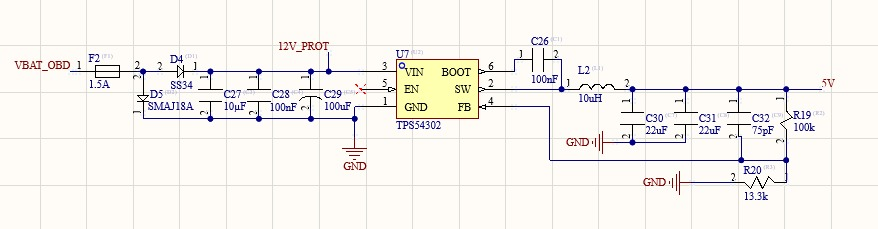
\includegraphics[width=1.02\textwidth]{Images/regu.png}
	
	\vspace{2mm}
	\small\raggedright
	\textit{Nota.} Diagrama eléctrico de la etapa de potencia regulada tipo reductora (\textit{Buck}) basada en el controlador TPS54302. Incluye las etapas de protección de entrada (fusible PTC rearmable, diodo Schottky de protección contra inversión de polaridad y diodo TVS), el filtro de potencia LC y el lazo de realimentación ajustado para una salida estable de 5~V/3~A.
\end{figure}

\begin{figure}[H]
	% Formato APA 7 con protección para el índice de figuras
	\captionsetup{labelformat=simple, labelsep=newline, textfont=it, labelfont=bf, justification=raggedright, singlelinecheck=false}
	\caption[Esquemático de los reguladores LDO AMS1117 y AP2112 en Altium Designer]{Esquemático del circuito de regulación lineal para la alimentación de 3.3~V.}
	\label{fig:esquematico_reg_3v3}
	\centering
	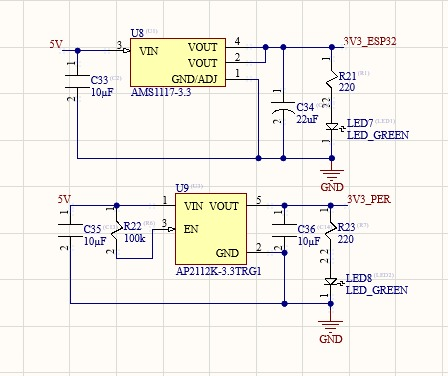
\includegraphics[width=0.8\textwidth]{Images/regum.png} % Modifica el nombre de la imagen si es necesario
	
	\vspace{2mm}
	\small\raggedright
	\textit{Nota.} Diagrama eléctrico de la etapa de regulación lineal que reduce el voltaje de 5~V a 3.3~V. El diseño emplea los reguladores de baja caída de tensión (LDO, por sus siglas en inglés) AMS1117 y AP2112 para suministrar energía de forma estable al microcontrolador y periféricos de 3.3~V. 
\end{figure}

\subsubsection{Sistema transceptor CAN}

Para la comunicación en el bus CAN, se seleccionó el transceptor SN65HVD230 (ver Tabla \ref{tab:componentes_seleccionados}). La configuración del circuito se realizó siguiendo las recomendaciones técnicas detalladas en su hoja de datos \citep{sn65hvd230_datasheet}, la cual describe la implementación óptima para garantizar la integridad de la señal. La configuración del esquema de conexión se ilustra en la Figura \ref{fig:sn65}

\begin{figure}[H]
	% Se usa labelformat=simple para que LaTeX gestione la numeración automáticamente
	\captionsetup{labelformat=simple, labelsep=period, textfont=it, labelfont=bf, justification=raggedright, singlelinecheck=false}
	
	\caption{Configuración de conexión óptima del transceptor CAN SN65HVD230}
	\label{fig:sn65}
	
	\vspace{4mm}
	% Imagen de la conexión del transceptor
	\centering
	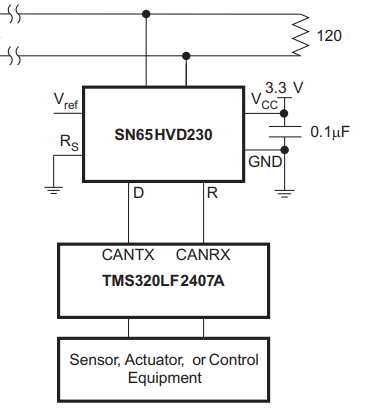
\includegraphics[width=0.40\textwidth]{Images/sn65.png}
	
	\vspace{4mm}
	% Nota a la izquierda
	\raggedright
	\small
	\textit{Nota.} Diagrama de conexión típica para el transceptor SN65HVD230, incluyendo la resistencia de terminación de 120 $\Omega$ entre las líneas CANH y CANL para evitar reflexiones en el bus, y la configuración de los pines de control para el modo de operación de alta velocidad. Adaptado de \citet{sn65hvd230_datasheet}.
\end{figure}

Tras analizar el esquema de los módulos basados en el SN65HVD230, se identificó una resistencia adicional conectada al pin RS (Rate Select). Asimismo, se añadió un PediScan, cuya función es actuar como un escáner y herramienta de diagnóstico automotriz, permitiendo la comunicación con la ECU del vehículo a través del puerto OBD-II para la lectura de parámetros, códigos de diagnóstico (DTC) y datos en tiempo real. Su incorporación permitió tomar como referencia un dispositivo comercial ampliamente utilizado para validar el diseño de la interfaz CAN implementada. Al integrar esta configuración en el diseño, el sistema resultante se ilustra en la Figura \ref{fig:esquema_can}.

\begin{figure}[H]
	% Formato APA 7 con protección para el índice de figuras
	\captionsetup{labelformat=simple, labelsep=newline, textfont=it, labelfont=bf, justification=raggedright, singlelinecheck=false}
	\caption[Esquemático del transceptor CAN SN65HVD230 en EasyEDA]{Esquemático del circuito transceptor CAN basado en el SN65HVD230.}
	\label{fig:esquema_can}
	\centering
	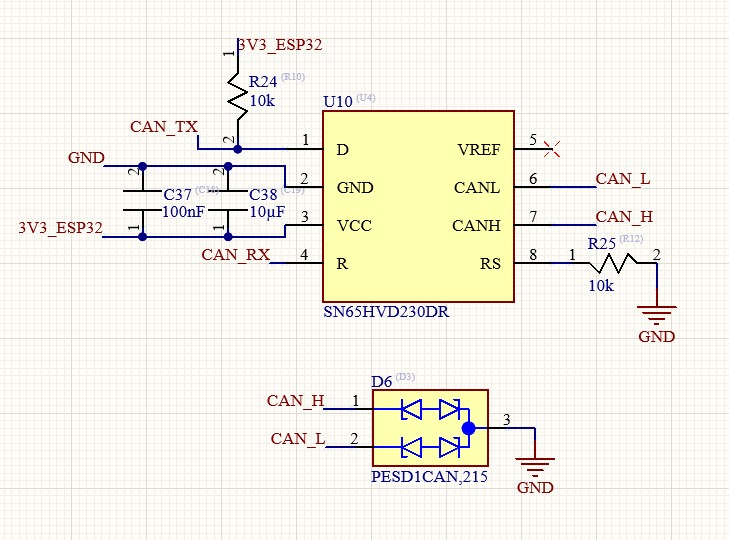
\includegraphics[width=0.9\textwidth]{Images/esquematico_can_final.png}
	
	\vspace{2mm}
	\small\raggedright
	\textit{Nota.} Diagrama eléctrico de la interfaz de comunicación CAN basada en el transceptor SN65HVD230. Incluye la configuración de los pines de control, la red de desacoplamiento de alimentación y la resistencia de terminación de 120 $\Omega$ necesaria para la integridad del bus, siguiendo las especificaciones de diseño recomendadas en la hoja de datos del fabricante.
\end{figure}


\subsubsection{Sistema de procesamiento}

Para este sistema se optó por el módulo \textbf{ESP32-S3-WROOM-1-N16R8}, el cual integra el microcontrolador ESP32-S3 de Espressif Systems. Este dispositivo incorpora un procesador de doble núcleo basado en la arquitectura Xtensa\textsuperscript{\textregistered} LX7 de hasta 240 MHz, conectividad Wi-Fi de 2.4 GHz y Bluetooth Low Energy (BLE) 5.0, además de una memoria Flash integrada de 16 MB y 8 MB de PSRAM. Estas características proporcionan la capacidad de ejecutar simultáneamente las tareas de adquisición de datos del vehículo, almacenamiento en memoria microSD, comunicación mediante el protocolo CAN y la implementación de un servidor web local para la visualización de información en tiempo real; el desempeño del sistema se mantiene estable incluso con estas tareas corriendo en paralelo \citep{espressif_esp32_datasheet}. Para asegurar el correcto funcionamiento del microcontrolador se debe implementar, además, la configuración mínima de hardware recomendada por el fabricante, tal como se ilustra en la Figura \ref{fig:conexion_minima_esp32}.

\begin{figure}[H]
	% Formato APA 7 con numeración automática gestionada por LaTeX
	\captionsetup{labelformat=simple, labelsep=newline, textfont=it, labelfont=bf, justification=raggedright, singlelinecheck=false}
	
	\caption{Circuito de conexión mínima y configuración óptima del módulo ESP32-S3-WROOM-1-N16R8.}
	\label{fig:conexion_minima_esp32}
	\centering
	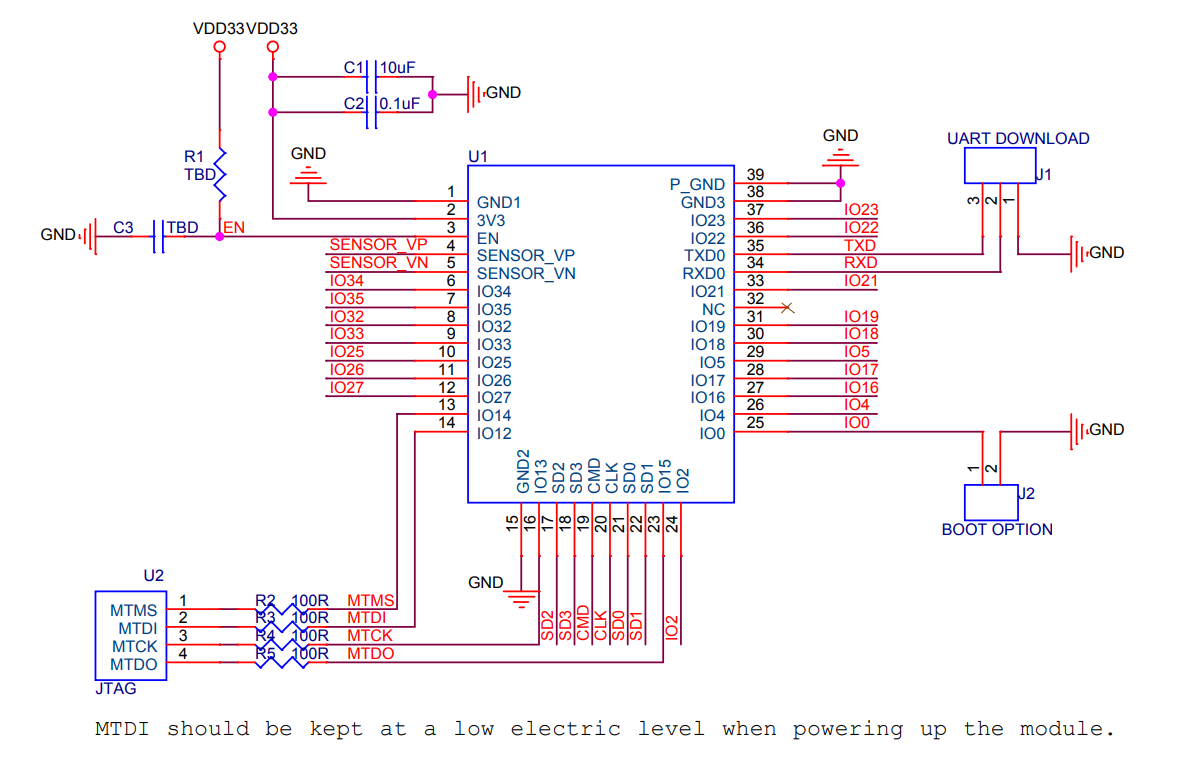
\includegraphics[width=1.02\textwidth]{Images/esp32_conexion_optima.png}
	
	\vspace{2mm}
	\small\raggedright
	\textit{Nota.} Esquemático de la configuración de hardware requerida para el correcto funcionamiento del módulo ESP32-S3-WROOM-1-N16R8. Se muestra el circuito de habilitación y reinicio mediante el pin EN, los condensadores de desacoplamiento de la alimentación de 3.3 V ubicados próximos al módulo, así como la configuración recomendada de los pines de arranque y programación para garantizar una inicialización estable del sistema. Adaptado de \textit{ESP32-S3-WROOM-1 Datasheet}, por Espressif Systems, 2024.
\end{figure}

La integración definitiva de la etapa de procesamiento se consolidó mediante el diseño del circuito impreso en la plataforma Altium Designer. Este esquema incorpora las recomendaciones establecidas por el fabricante para el módulo ESP32-S3-WROOM-1-N16R8 y la integración de los diferentes periféricos empleados en el sistema, optimizando la distribución de las señales de alimentación, comunicación y control para mejorar la estabilidad eléctrica y el rendimiento general del dispositivo. El resultado de esta integración y la topología eléctrica final del sistema basado en el microcontrolador se presentan detalladamente en la Figura \ref{fig:esp32fin}.

\begin{figure}[H]
	% Formato APA 7 con protección para el índice de figuras
	\captionsetup{labelformat=simple, labelsep=newline, textfont=it, labelfont=bf, justification=raggedright, singlelinecheck=false}
	\caption[Esquemático final del módulo ESP32-S3-WROOM-1-N16R8 en EasyEDA]{Esquemático completo del circuito de control y periféricos basados en el ESP32-S3-WROOM-1-N16R8.}
	\label{fig:esp32fin}
	\centering
	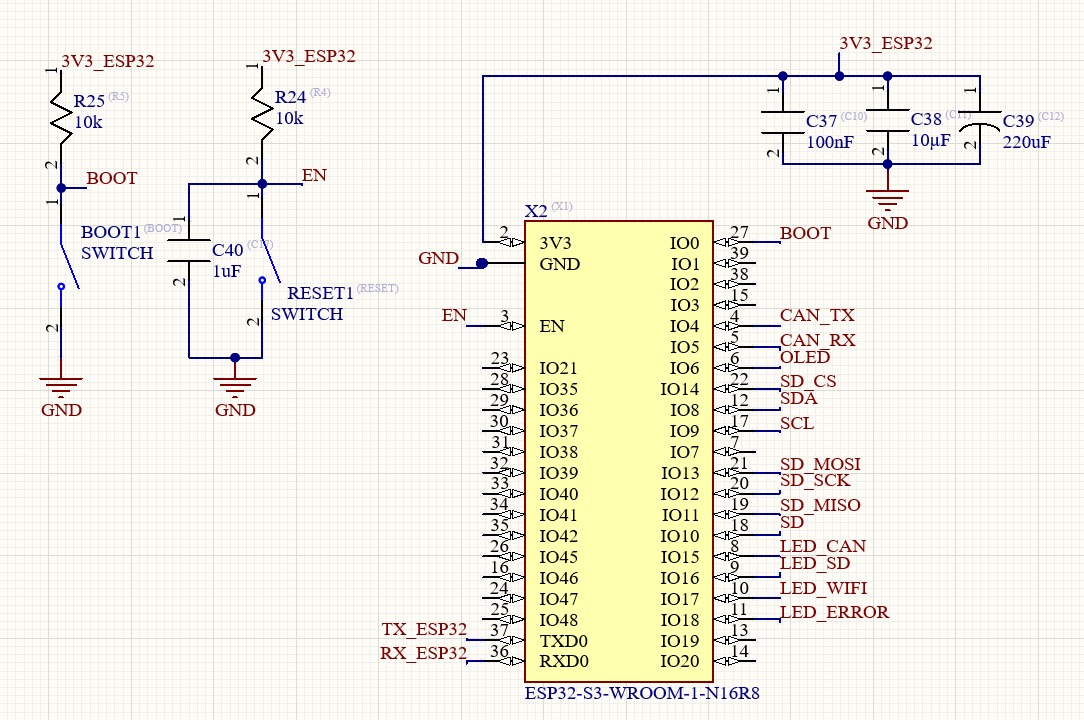
\includegraphics[width=1.02\textwidth]{Images/ESP32_FINAL.png}
	
	\vspace{2mm}
	\small\raggedright
	\textit{Nota.} Diagrama eléctrico final desarrollado en Altium Designer para la etapa de procesamiento basada en el módulo ESP32-S3-WROOM-1-N16R8. El diseño integra las recomendaciones de la hoja de datos del fabricante, el acondicionamiento de la alimentación, el circuito de programación y reinicio automático, así como la conexión de los periféricos utilizados en el sistema para garantizar un funcionamiento confiable durante la adquisición, procesamiento y visualización de los datos obtenidos desde el puerto OBD-II.
\end{figure}


\subsubsection{Sistema de visualización}

Una vez definida la distribución de señales del conector de expansión, se procedió al diseño del esquemático de la etapa de visualización utilizando el software Altium Designer. En este diseño se integran la pantalla OLED, el conector JST-GH, las resistencias \textit{pull-up} del bus $I^2C$ y el condensador de desacoplamiento, obteniéndose el circuito mostrado en la Figura \ref{fig:esquematico_visualizacion}.

\begin{table}[H]
	\centering
	\captionsetup{labelformat=simple, labelsep=newline, textfont=it, labelfont=bf, justification=raggedright, singlelinecheck=false}
	\caption{Asignación de pines y código de colores del conector de expansión de 6 pines}
	\label{tab:pinout_conector}
	\small
	\renewcommand{\arraystretch}{1.3}
	% Mantenemos la calibración exacta de anchos fijos (3.5cm + 2.0cm + 8.7cm = 14.2cm)
	\begin{tabular}{p{3.5cm} p{2.0cm} p{8.7cm}}
		\toprule
		\rowcolor[rgb]{0.851, 0.851, 0.851}
		\textbf{Pin / Función} & \textbf{Color} & \textbf{Descripción} \\
		\midrule
		\texttt{VCC} & Rojo & Alimentación principal del módulo externo regulada a 3{,}3~V. \\
		\texttt{GND} & Negro & Referencia común de tierra del sistema. \\
		\texttt{SCL} & Verde & Línea de reloj de la interfaz de comunicación serial $I^2C$. \\
		\texttt{SDA} & Azul & Línea de datos bidireccional de la interfaz de comunicación serial $I^2C$. \\
		\bottomrule
	\end{tabular}
	\vspace{0.2cm}
	\begin{flushleft}
		\small
		\begin{center}
			\textit{Nota.} La distribución de señales del conector de expansión garantiza la compatibilidad con sensores periféricos a través del bus de comunicación $I^2C$. Las líneas auxiliares permiten la integración posterior de interrupciones de hardware o señales de control adicionales sin necesidad de modificar el diseño base del circuito impreso.
		\end{center}
	\end{flushleft}
\end{table}

Definida el uso de este conector se procede a dibujar el esquemático (ver Figura \ref{fig:esquematico_visualizacion}) donde su conexión sera al oled.

\begin{figure}[H]
	% Formato APA 7 con protección para el índice de figuras (Mismo estilo de tus otras figuras de EasyEDA)
	\captionsetup{labelformat=simple, labelsep=newline, textfont=it, labelfont=bf, justification=raggedright, singlelinecheck=false}
	\caption[Esquemático de la etapa de visualización OLED en EasyEDA]{Esquemático del circuito de visualización física y conector de expansión periférico.}
	\label{fig:esquematico_visualizacion}
	\centering
	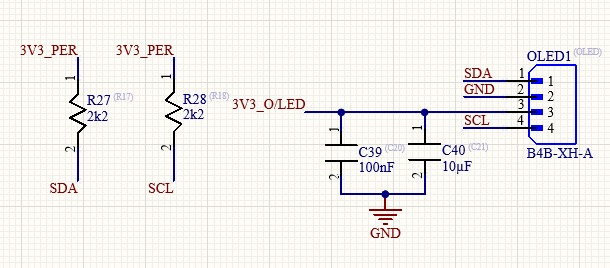
\includegraphics[width=0.9\textwidth]{Images/visu.png}
	
	\vspace{2mm}
	\small\raggedright
	\textit{Nota.} \textit{Nota.} Diagrama esquemático desarrollado en Altium Designer para la etapa de visualización del sistema. El diseño incorpora la pantalla OLED, el conector JST-GH de seis pines para su conexión externa, las resistencias \textit{pull-up} de las líneas SDA y SCL del bus $I^2C$, así como el condensador de desacoplamiento de 100~nF ubicado próximo al periférico para mejorar la estabilidad de la alimentación y la integridad de la comunicación en aplicaciones con cableado de mayor longitud..
\end{figure}

\subsubsection{Sistema de almacenamiento de datos}

Con el propósito de almacenar de forma local los datos obtenidos desde el sistema OBD-II, se incorporó una memoria MicroSD al diseño electrónico. Su utilización permite registrar de manera permanente las variables adquiridas por el ESP32-S3-WROOM-1-N16R8, facilitando el almacenamiento de grandes volúmenes de información para su posterior análisis sin depender de una conexión inalámbrica o de un servidor externo. Esta característica resulta especialmente útil durante las pruebas de campo, donde es necesario conservar el historial completo de los parámetros del vehículo para realizar comparaciones, validar modelos matemáticos y analizar el comportamiento del sistema en diferentes condiciones de operación.

La implementación de esta etapa se basó en las especificaciones de la SD Card Association \citep{transcend_microsd_datasheet}. Debido a que tanto el módulo ESP32-S3-WROOM-1-N16R8 como las tarjetas MicroSD operan con niveles lógicos de 3.3 V, fue posible realizar la conexión directa entre ambos dispositivos sin necesidad de incorporar convertidores de nivel lógico, simplificando el diseño y reduciendo el número de componentes.

Para la comunicación entre el microcontrolador y la memoria se seleccionó el protocolo SPI (Serial Peripheral Interface), debido a su elevada velocidad de transferencia, simplicidad de implementación y reducido número de líneas de comunicación. En esta configuración se emplean las señales SCK, MOSI, MISO y CS para gestionar el acceso a la memoria durante las operaciones de lectura y escritura.

Con el objetivo de garantizar un funcionamiento confiable del sistema, se incorporaron condensadores de desacoplamiento de 10~$\mu$F y 100~nF próximos al conector MicroSD. El condensador de 10~$\mu$F proporciona una reserva de energía para compensar los picos de corriente que se presentan durante las operaciones de escritura, mientras que el condensador cerámico de 100~nF filtra las componentes de alta frecuencia presentes en la alimentación, reduciendo el ruido eléctrico y mejorando la estabilidad del sistema.

También se implementaron resistencias de 10~k$\Omega$ conectadas a las líneas DAT1, DAT2 y DAT3/CS de la tarjeta MicroSD. Estas resistencias mantienen dichas líneas en un nivel lógico alto cuando no están siendo utilizadas, evitando estados flotantes durante el encendido del sistema, la inserción o extracción de la tarjeta y mejorando la confiabilidad del proceso de inicialización, de acuerdo con las recomendaciones de diseño para dispositivos compatibles con tarjetas SD. El esquema eléctrico final de esta etapa se presenta en la Figura \ref{fig:esquematico_microsd}.

\begin{figure}[H]
	\captionsetup{labelformat=simple, labelsep=newline, textfont=it, labelfont=bf, justification=raggedright, singlelinecheck=false}
	\caption[Esquemático del sistema de almacenamiento mediante memoria MicroSD en Altium Designer]{Esquemático de la etapa de almacenamiento de datos mediante tarjeta MicroSD.}
	\label{fig:esquematico_microsd}
	\centering
	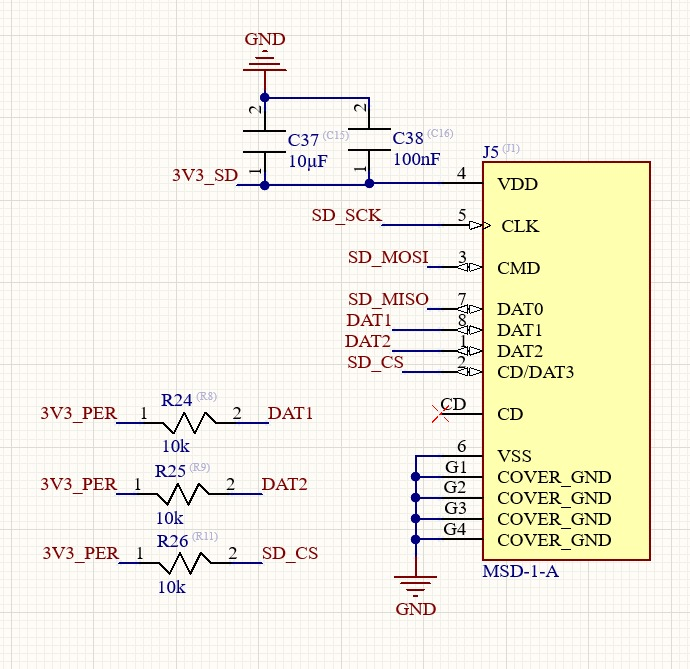
\includegraphics[width=0.75\textwidth]{Images/sd.png}
	
	\vspace{2mm}
	\small\raggedright
	\textit{Nota.} Diagrama esquemático desarrollado en Altium Designer para la interfaz de almacenamiento mediante memoria MicroSD. El diseño incorpora los condensadores de desacoplamiento de 10~$\mu$F y 100~nF para estabilizar la alimentación durante las operaciones de lectura y escritura, así como resistencias de 10~k$\Omega$ conectadas a las líneas DAT1, DAT2 y DAT3/CS, las cuales mantienen dichas señales en un estado lógico definido durante el arranque e inicialización de la tarjeta, incrementando la confiabilidad de la comunicación SPI con el módulo ESP32-S3-WROOM-1-N16R8.
\end{figure}

\subsubsection{Sistema de programación de uso de periféricos}

\subsubsection{Control de alimentación de periféricos}

Con el propósito de optimizar el consumo energético del sistema y permitir una administración independiente de los dispositivos auxiliares, se incorporó un interruptor electrónico de carga TPS22918. Este circuito integrado permite conectar o desconectar la alimentación de los periféricos mediante una señal de control proveniente del microcontrolador ESP32-S3-WROOM-1-N16R8.

En el diseño propuesto, dos pines GPIO del ESP32-S3 controlan el estado lógico de habilitación del TPS22918, permitiendo energizar únicamente los dispositivos cuando son requeridos por la aplicación. Los principales periféricos alimentados mediante este circuito son la memoria MicroSD y la pantalla OLED, los cuales permanecen desenergizados durante el proceso de inicialización del sistema o cuando no se encuentran en uso; así se reduce el consumo de corriente y se evitan inicializaciones indeseadas.

La utilización del TPS22918 también proporciona un encendido controlado de los periféricos gracias a su baja resistencia de conducción (\textit{R\textsubscript{ON}}) y a su mecanismo interno de control de la corriente de irrupción (\textit{Inrush Current}) (ver Apéndice L), evitando caídas bruscas de tensión sobre la línea de alimentación de 3.3 V durante la conexión de cargas capacitivas. Estas características contribuyen a mejorar la estabilidad del sistema y la confiabilidad del funcionamiento del microcontrolador durante el arranque y la operación normal.

El esquemático correspondiente a la etapa de control de alimentación se presenta en la Figura \ref{fig:esquematico_programacion}.

\begin{figure}[H]
	\captionsetup{labelformat=simple, labelsep=newline, textfont=it, labelfont=bf, justification=raggedright, singlelinecheck=false}
	\caption[Esquemático del control de alimentación de periféricos]{Esquemático de la etapa de control de alimentación mediante el interruptor electrónico TPS22918.}
	\label{fig:esquematico_programacion}
	\centering
	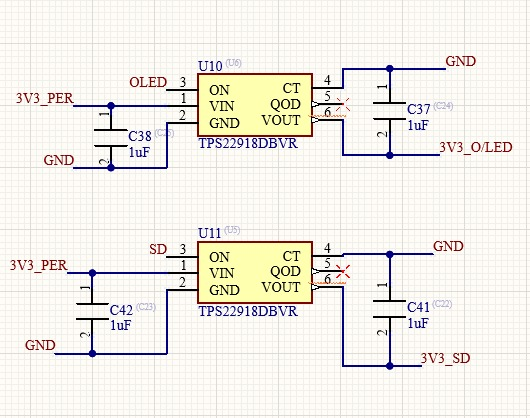
\includegraphics[width=0.82\textwidth]{Images/PROGRAMACION.png}
	
	\vspace{2mm}
	\small\raggedright
	\textit{Nota.} Diagrama esquemático desarrollado en Altium Designer para el control de alimentación de los periféricos del sistema. El circuito emplea un interruptor electrónico TPS22918, controlado mediante señales GPIO del módulo ESP32-S3-WROOM-1-N16R8, para habilitar o deshabilitar la alimentación de la memoria MicroSD y la pantalla OLED. Esta estrategia permite reducir el consumo energético, controlar la secuencia de encendido de los periféricos y mejorar la estabilidad de la línea de alimentación de 3.3 V al limitar la corriente de irrupción durante la conexión de las cargas.
\end{figure}

\subsubsection{Sistema de monitoreo y estado}

\subsubsection{Indicadores de estado}

Con el propósito de facilitar el diagnóstico visual y el monitoreo del estado operativo del sistema, se incorporó un conjunto de indicadores luminosos basados en diodos emisores de luz (LED) de montaje superficial (SMD). Estos indicadores permiten conocer de forma inmediata el estado de los principales módulos del dispositivo durante su funcionamiento: las tareas de depuración, mantenimiento y validación del sistema pueden hacerse así sin herramientas externas de diagnóstico.

Cada LED es controlado mediante un pin de propósito general (GPIO) del módulo ESP32-S3-WROOM-1-N16R8, permitiendo que el firmware indique diferentes estados de operación de acuerdo con los eventos generados por el sistema. Para limitar la corriente que circula por cada diodo y proteger tanto los LED como las salidas digitales del microcontrolador, se incorporó una resistencia de 220~$\Omega$ conectada en serie con cada indicador.

El sistema de señalización está conformado por los siguientes indicadores:

\begin{itemize}
	\item \textbf{LED CAN (morado):} Indica la actividad de comunicación sobre el bus CAN, encendiéndose o parpadeando durante la transmisión y recepción de tramas provenientes de la ECU del vehículo.
	
	\item \textbf{LED MicroSD (naranja):} Señaliza las operaciones de acceso a la memoria MicroSD, incluyendo procesos de inicialización, lectura y escritura de archivos de registro.
	
	\item \textbf{LED ERROR (rojo):} Indica la presencia de fallas detectadas por el sistema, como errores de comunicación, problemas durante la inicialización de los periféricos o cualquier condición anómala registrada por el firmware.
	
	\item \textbf{LED Wi-Fi (azul):} Muestra el estado de la conectividad inalámbrica y del servidor web local implementado en el ESP32-S3, indicando la disponibilidad del sistema para la visualización de datos mediante un navegador web.
\end{itemize}

El esquemático correspondiente a esta etapa se desarrolló en Altium Designer y se presenta en la Figura \ref{fig:esquematico_indicadores}.

\begin{figure}[H]
	\captionsetup{labelformat=simple, labelsep=newline, textfont=it, labelfont=bf, justification=raggedright, singlelinecheck=false}
	\caption[Esquemático del sistema de indicadores visuales]{Esquemático del circuito de indicadores LED para el monitoreo del estado del sistema.}
	\label{fig:esquematico_indicadores}
	\centering
	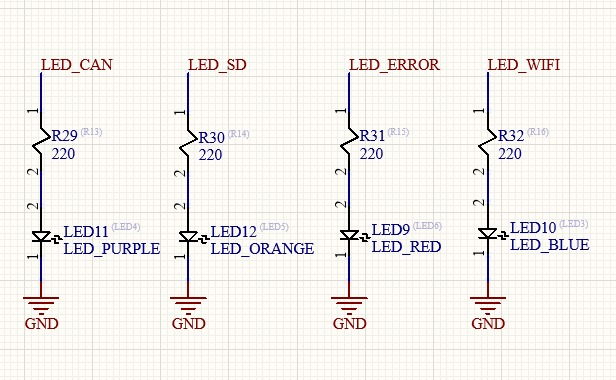
\includegraphics[width=0.82\textwidth]{Images/INDICADOR.png}
	
	\vspace{2mm}
	\small\raggedright
	\textit{Nota.} Diagrama esquemático desarrollado en Altium Designer para el sistema de indicadores visuales. Cada LED se encuentra conectado a un GPIO del módulo ESP32-S3-WROOM-1-N16R8 mediante una resistencia limitadora de 220~$\Omega$, la cual restringe la corriente que circula por el diodo, protege las salidas digitales del microcontrolador y prolonga la vida útil de los indicadores. Los cuatro LED permiten visualizar el estado de la comunicación CAN, la actividad de la memoria MicroSD, la conectividad Wi-Fi y la presencia de condiciones de error detectadas durante el funcionamiento del sistema.
\end{figure}

\subsection{Placa preliminar (EasyEDA)}
\label{sec:pcb_preliminar_diseno}

Antes de proceder con el diseño de la placa final descrito en el resto de esta sección, se desarrolló en EasyEDA una placa preliminar que replica el mismo circuito ya validado sobre protoboard (Capítulo~4, Sección~4.1.3), con el fin de contar con una versión física más robusta que las conexiones sueltas de una protoboard para las pruebas de campo. A diferencia de la placa final, esta versión preliminar resuelve la alimentación con un regulador lineal simple (7805 más un transistor de paso TIP42C en configuración de refuerzo de corriente) en lugar de la conversión conmutada de dos rieles, y conecta el transceptor CAN, la pantalla OLED y el módulo microSD --ya validados en la etapa de protoboard-- mediante conectores de pines en vez de integrarlos directamente en la placa. El esquemático completo se muestra en la Figura~\ref{fig:esquematico_pcb_preliminar}.

\begin{figure}[H]
	\captionsetup{labelformat=simple, labelsep=newline, textfont=it, labelfont=bf, justification=raggedright, singlelinecheck=false}
	\caption[Esquemático de la placa preliminar en EasyEDA]{Esquemático completo de la placa preliminar.}
	\label{fig:esquematico_pcb_preliminar}
	\centering
	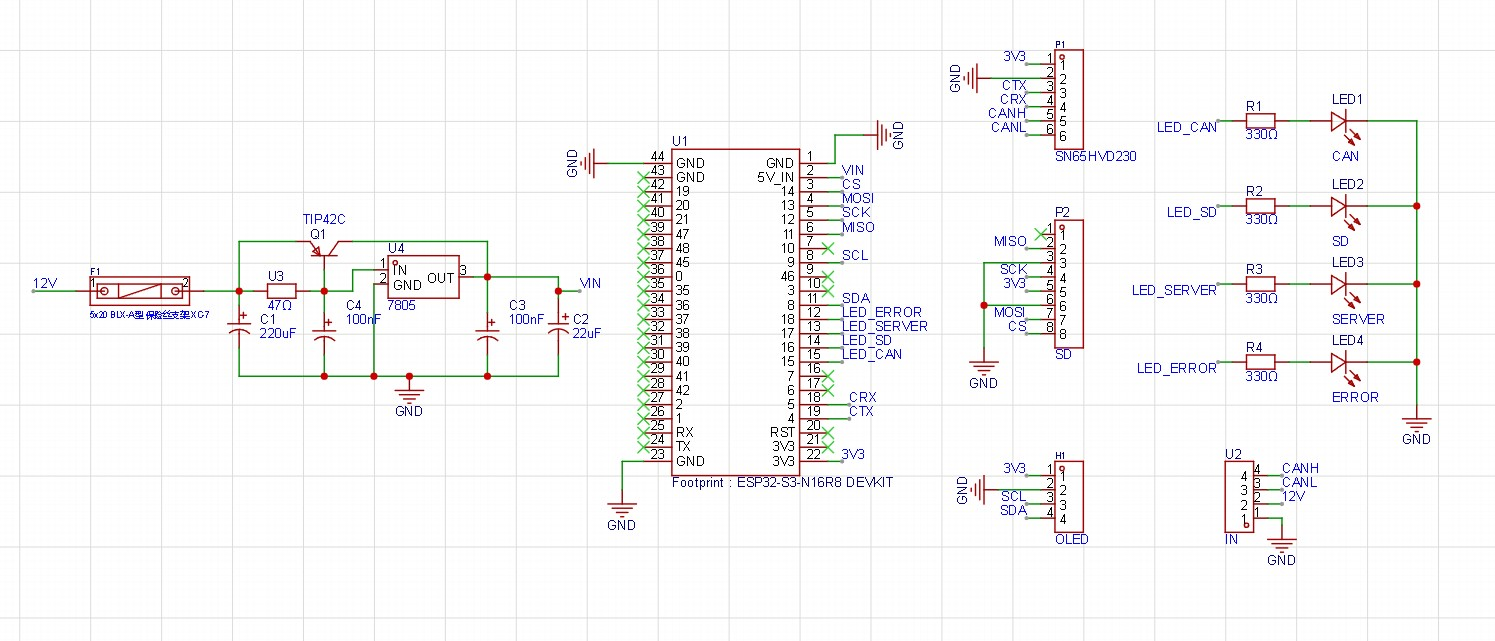
\includegraphics[width=0.95\textwidth]{Images/esquematico_pcb_proto.jpg}

	\vspace{2mm}
	\small\raggedright
	\textit{Nota.} Desarrollado en EasyEDA. El costo detallado de cada componente se presenta en el Capítulo~5 (Tabla~\ref{tab:costo_placa_preliminar_bom}).
\end{figure}

La Figura~\ref{fig:simulacion_pcb_preliminar} muestra la vista 3D generada por EasyEDA a partir de ese esquemático y del enrutado de la placa, previo al envío a fabricar.

\begin{figure}[H]
	\captionsetup{labelformat=simple, labelsep=newline, textfont=it, labelfont=bf, justification=raggedright, singlelinecheck=false}
	\caption[Vista 3D de la placa preliminar en EasyEDA]{Simulación 3D de la placa preliminar, generada en EasyEDA antes de la fabricación.}
	\label{fig:simulacion_pcb_preliminar}
	\centering
	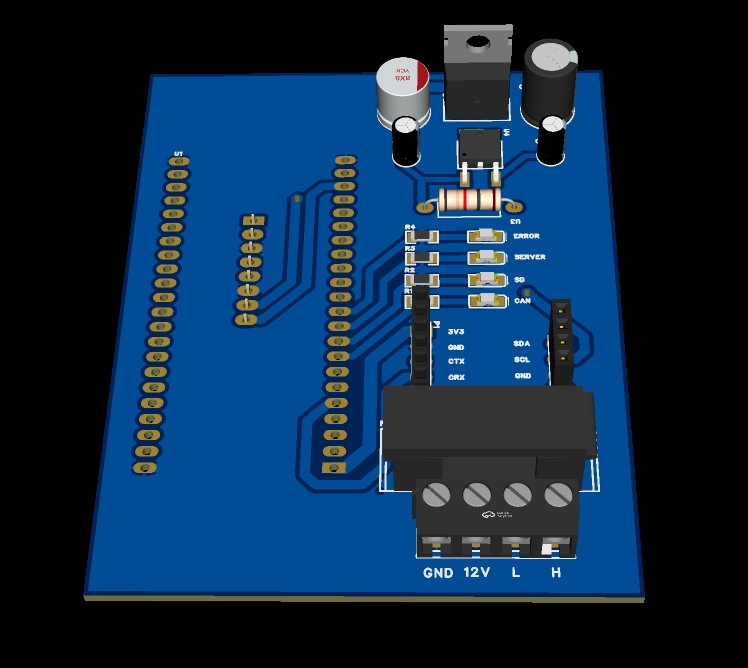
\includegraphics[width=0.55\textwidth]{Images/simulacion_pcb_proto.jpg}
\end{figure}

La fabricación de la placa preliminar se encargó a Robokit (La Paz); la Figura~\ref{fig:fisica_pcb_preliminar} muestra las caras superior e inferior de la placa recibida, previo al ensamblaje de los componentes.

\begin{figure}[H]
	\centering
	\caption{Placa preliminar fabricada por Robokit, sin ensamblar}
	\label{fig:fisica_pcb_preliminar}
	\begin{subfigure}[t]{0.48\textwidth}
		\centering
		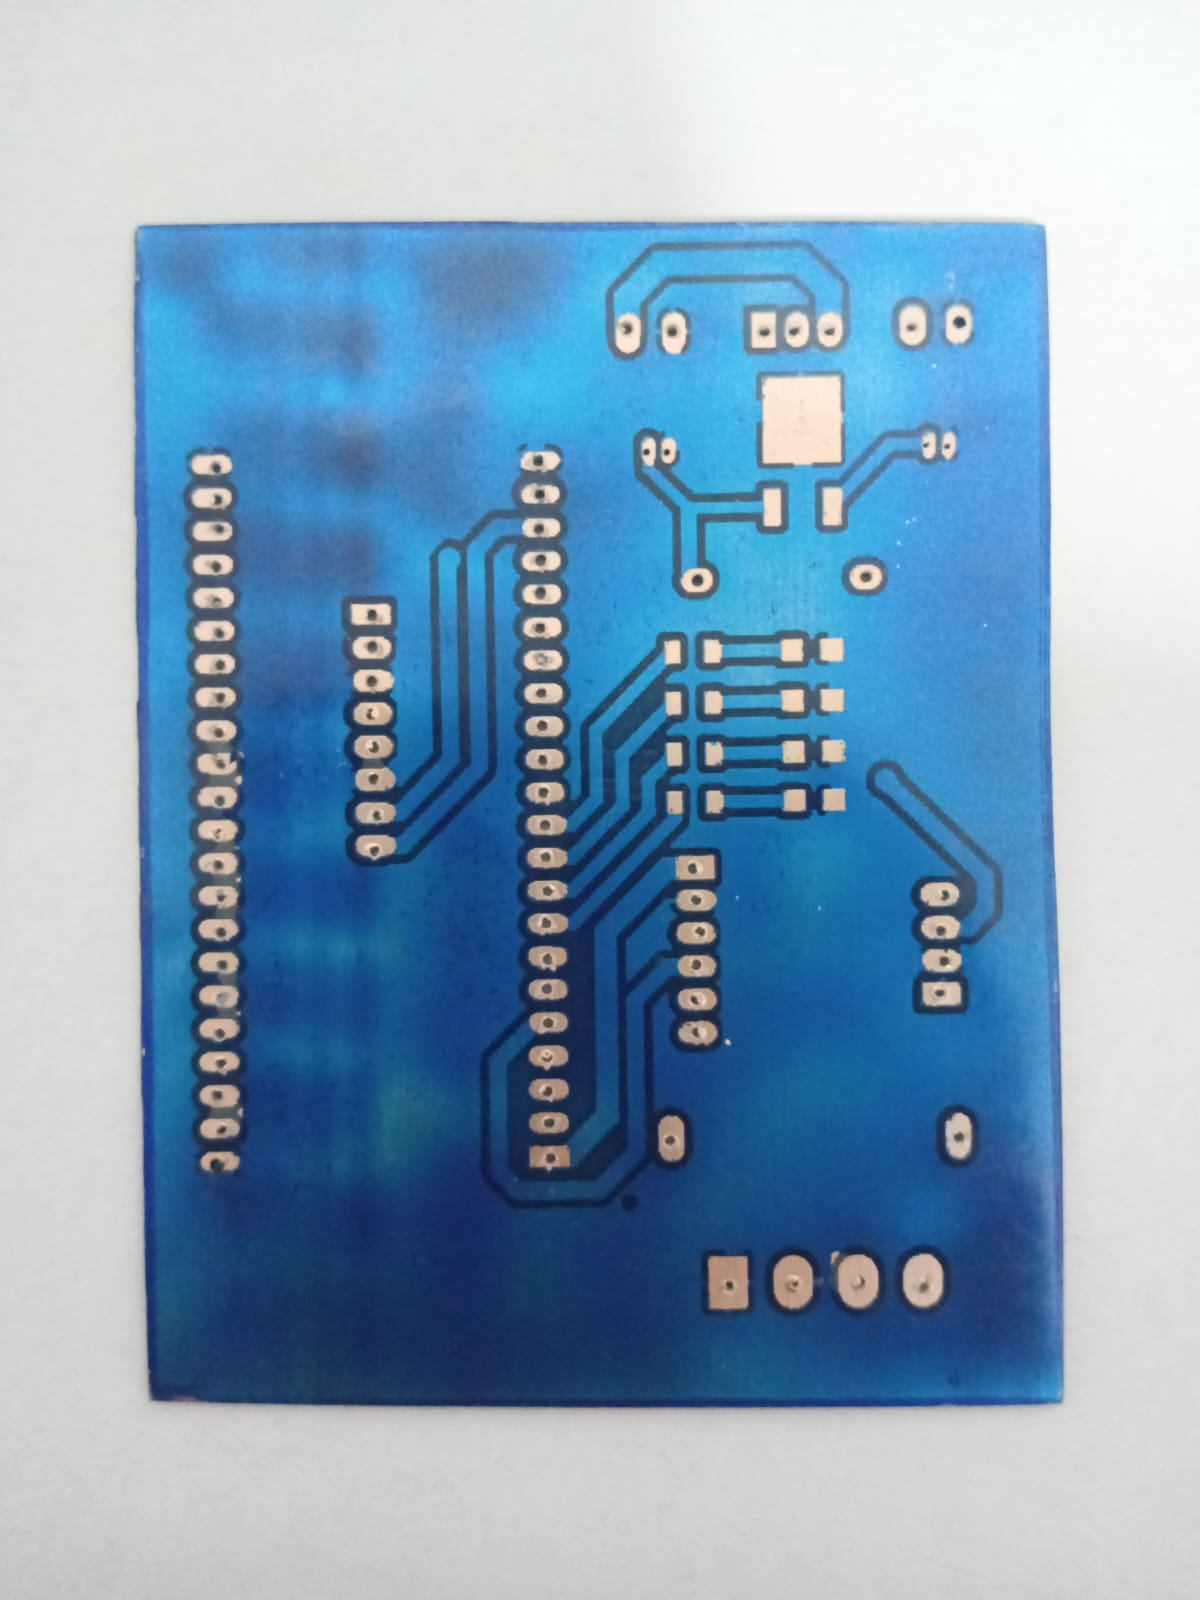
\includegraphics[width=\textwidth]{Images/top_pcb_proto.jpeg}
		\caption{Cara superior (\textit{top})}
		\label{fig:top_pcb_preliminar}
	\end{subfigure}
	\hfill
	\begin{subfigure}[t]{0.48\textwidth}
		\centering
		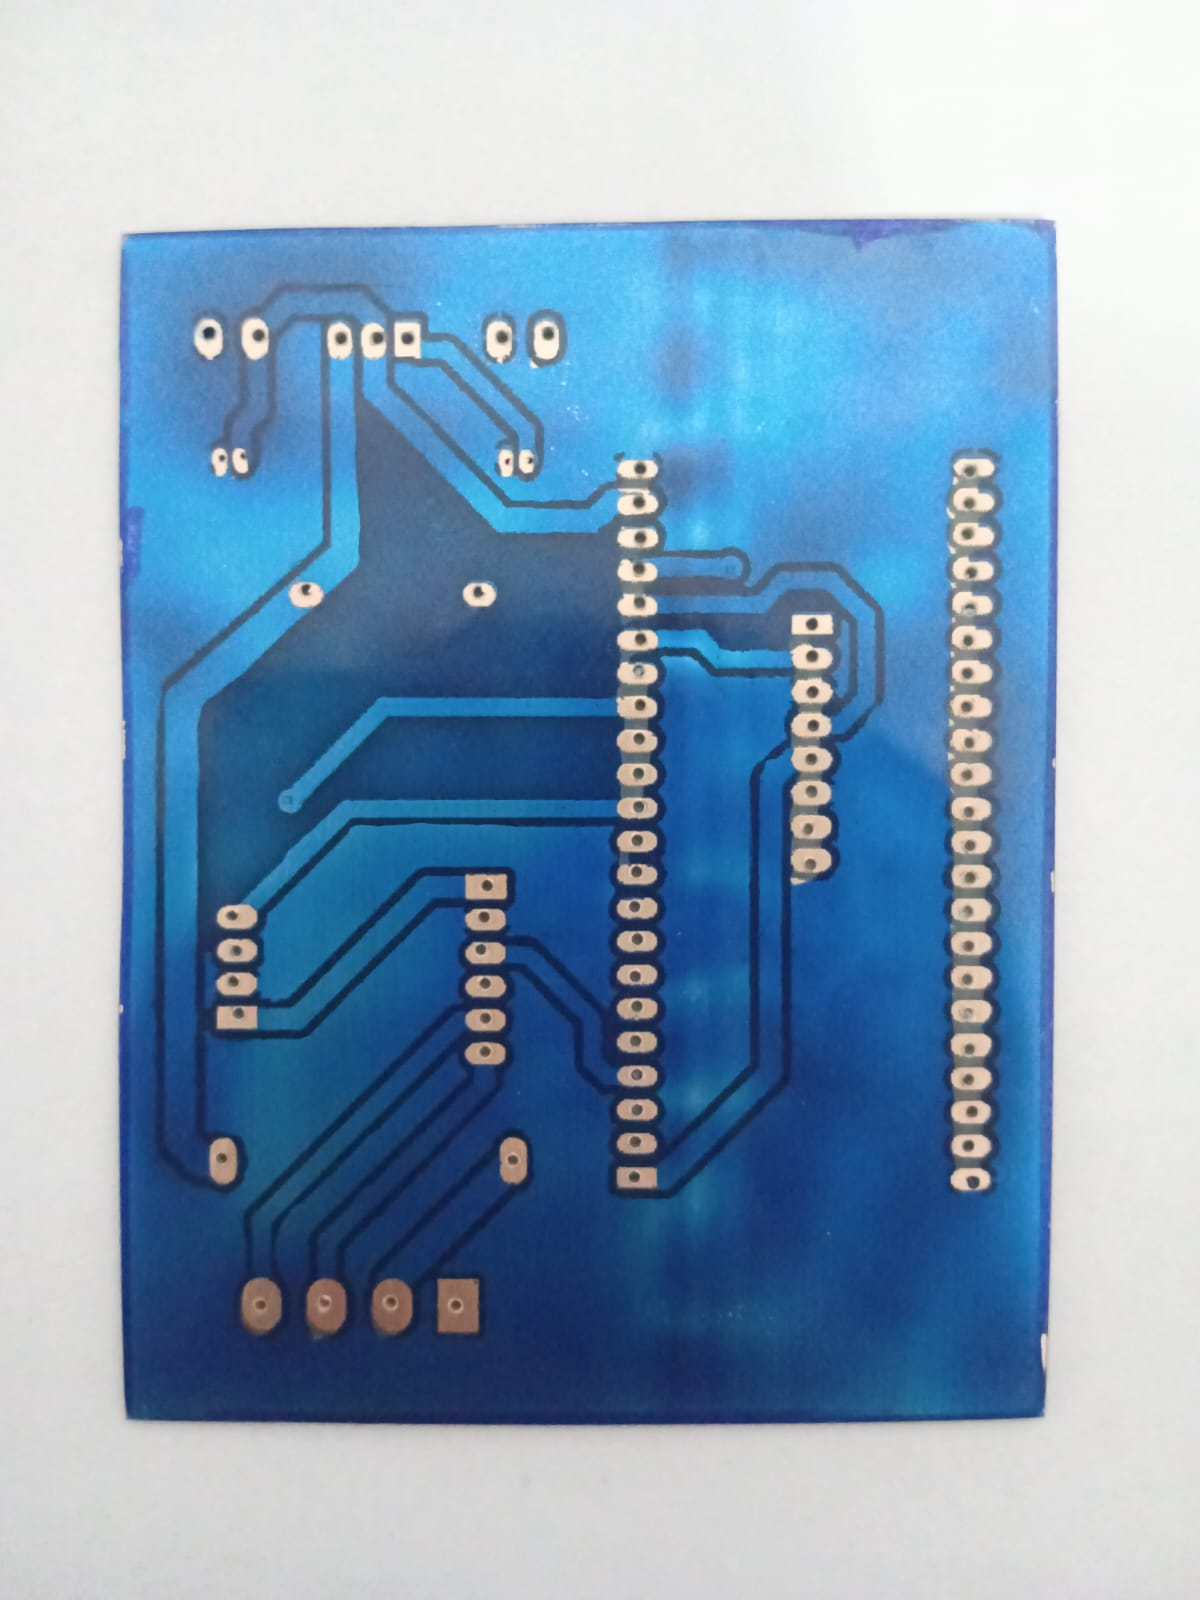
\includegraphics[width=\textwidth]{Images/bottom_pcb_proto.jpeg}
		\caption{Cara inferior (\textit{bottom})}
		\label{fig:bottom_pcb_preliminar}
	\end{subfigure}
	\vspace{2pt}
	\\
	{\footnotesize\textit{Nota.} Placa de una sola cara fabricada por Robokit (La Paz), 150\,Bs (Capítulo~5, Tabla~\ref{tab:costo_pcb_preliminar}); el ensamblaje de los componentes se realizó manualmente. Elaboración propia.}
\end{figure}

Una vez soldados los componentes de la Tabla~\ref{tab:costo_placa_preliminar_bom} (Capítulo~5) sobre esta placa, y reutilizando el módulo ESP32-S3, el transceptor SN65HVD230 y la pantalla OLED ya validados en protoboard, se obtiene la placa ensamblada de la Figura~\ref{fig:ensamblada_pcb_preliminar}.

\begin{figure}[H]
	\centering
	\caption{Placa preliminar ensamblada}
	\label{fig:ensamblada_pcb_preliminar}
	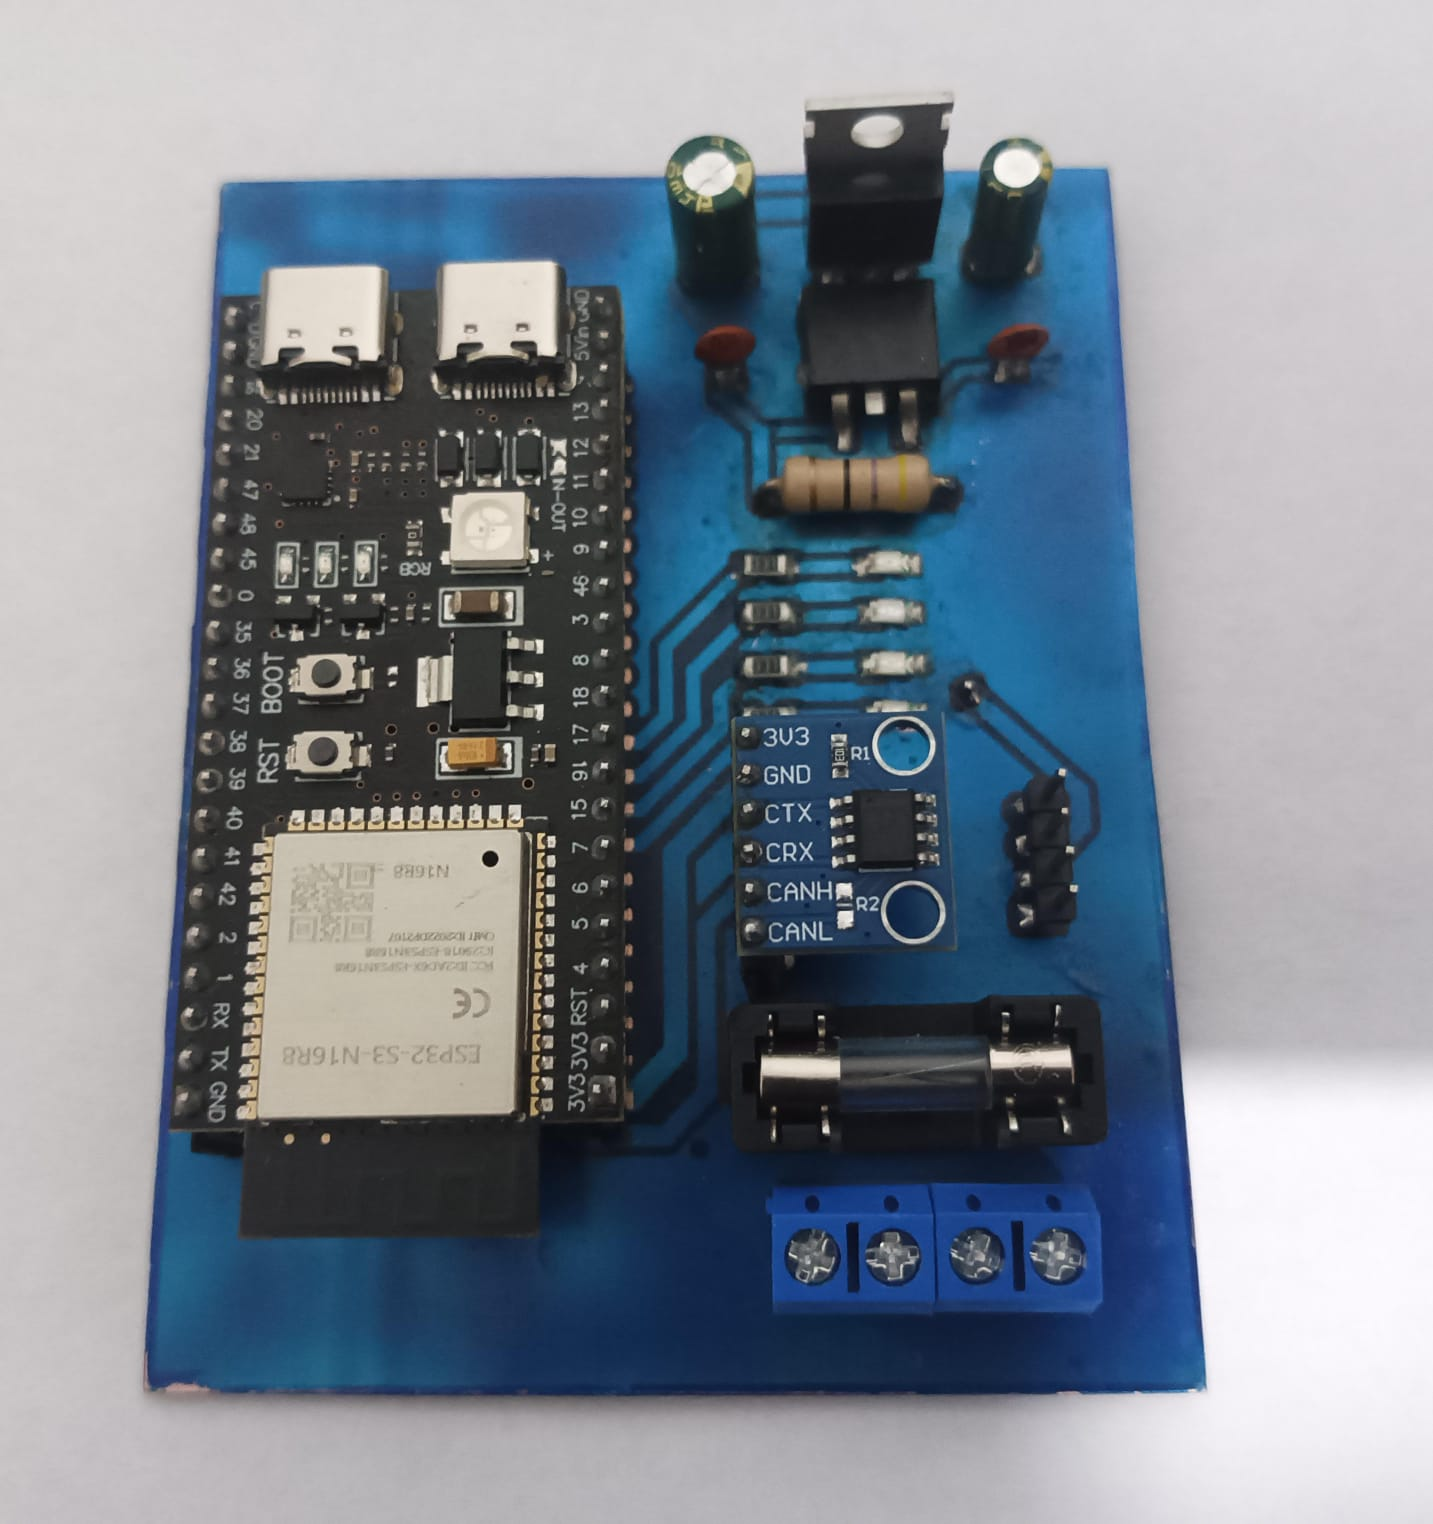
\includegraphics[width=0.6\textwidth]{Images/pcb_proto_ensamblada.jpeg}

	\vspace{2pt}
	{\footnotesize\textit{Nota.} Placa preliminar tras el ensamblaje manual de los componentes: se distinguen el módulo ESP32-S3-N16R8, el regulador 7805 con el transistor de paso TIP42C, el módulo transceptor SN65HVD230 (conectado mediante el header de 6 pines), el fusible reseteable F1 y el conector de entrada de 4 pines (GND, 12~V, CAN\_L, CAN\_H). Elaboración propia.}
\end{figure}

\subsection{Diseño de la carcasa del prototipo (impresión 3D)}
\label{sec:carcasa_prototipo}

Para esta presentación se diseñó e imprimió una carcasa únicamente para la placa preliminar; la carcasa de la placa final queda pendiente y se elaborará si el tribunal la solicita. Como punto de partida se tomó un modelo STL de una caja de dos piezas (base y tapa) publicado en MakerWorld, el repositorio de modelos de Bambu Lab, mostrado en la Figura~\ref{fig:stl_makerworld}.

\begin{figure}[H]
	\centering
	\caption{Modelo STL base, tomado de MakerWorld}
	\label{fig:stl_makerworld}
	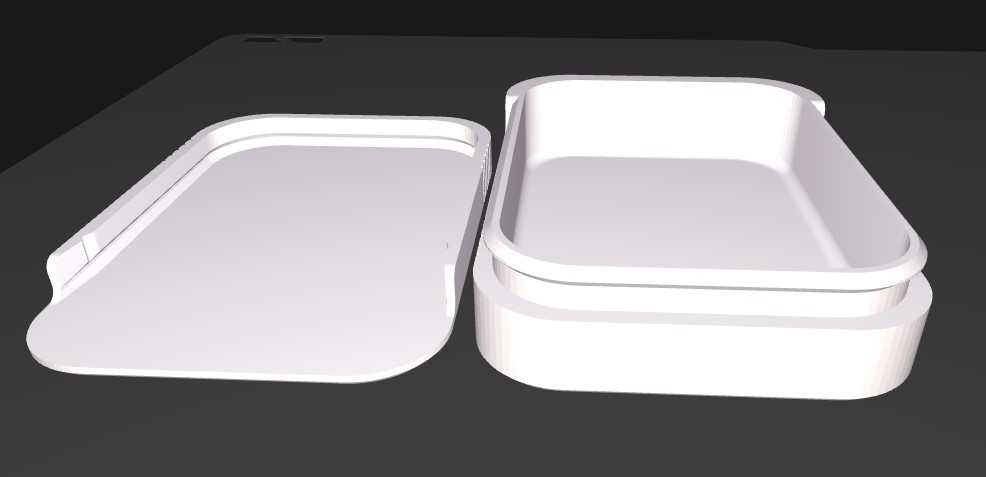
\includegraphics[width=0.7\textwidth]{Images/STL_MAKEWORD.jpg}

	\vspace{2pt}
	{\footnotesize\textit{Nota.} Modelo de caja de dos piezas (base y tapa) publicado en MakerWorld (Bambu Lab), usado como punto de partida antes de la edición en SolidWorks.}
\end{figure}

La tapa del modelo original no contaba con una abertura para la pantalla OLED; se editó en SolidWorks para agregar el recorte rectangular necesario, manteniendo el resto de la geometría del modelo original (Figura~\ref{fig:tapa_editada}).

\begin{figure}[H]
	\centering
	\caption{Tapa modificada en SolidWorks, con abertura para la pantalla OLED}
	\label{fig:tapa_editada}
	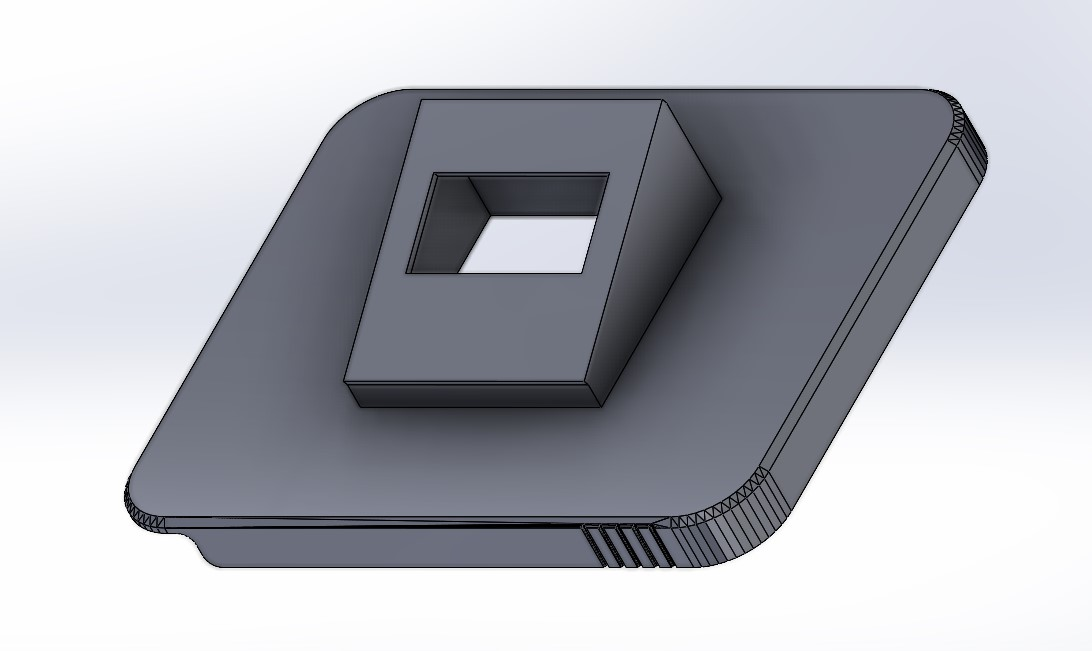
\includegraphics[width=0.6\textwidth]{Images/TAPA_EDITADA.jpg}
\end{figure}

La impresión se realizó en PLA, con una impresora propia Creality Ender V3 KE (Figura~\ref{fig:impresion_3d}). Se eligió PLA en vez de un material más resistente a la intemperie (por ejemplo, PETG o ABS) porque, al tratarse de una carcasa de prototipo, no está expuesta al sol de forma prolongada; esa consideración sí sería relevante para una carcasa de producción instalada de forma permanente en el vehículo.

\begin{figure}[H]
	\centering
	\caption{Impresión 3D en la Creality Ender V3 KE}
	\label{fig:impresion_3d}
	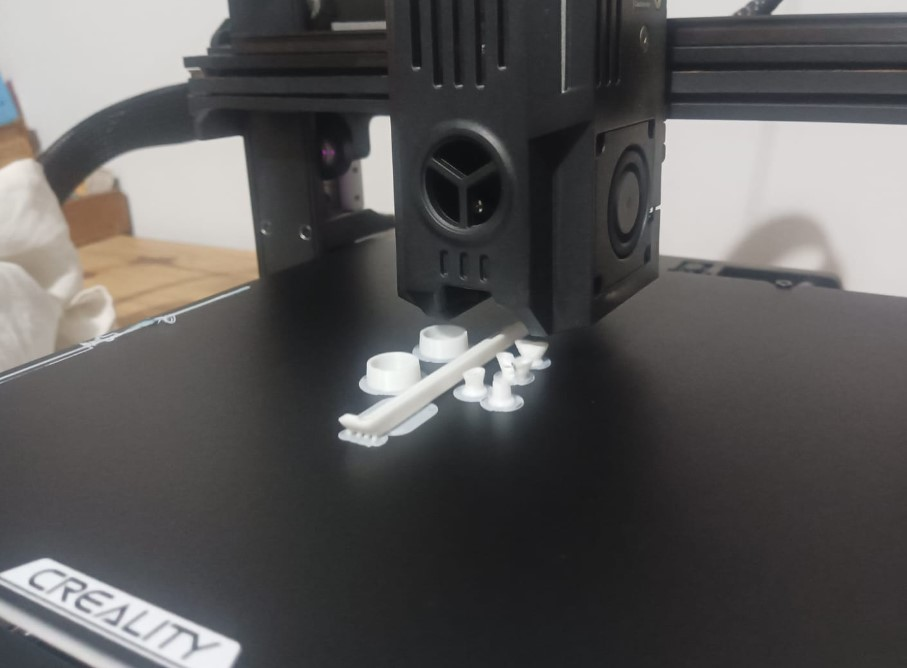
\includegraphics[width=0.7\textwidth]{Images/IMPRESION_3D.jpg}
\end{figure}

La base ya impresa (21~g de PLA) se muestra en la Figura~\ref{fig:carcasa_3d}; la tapa (16~g) está pendiente de impresión al momento de escribir este capítulo. El costo del material se presenta en el Capítulo~5 (Tabla~\ref{tab:costo_carcasa}).

\begin{figure}[H]
	\centering
	\caption{Carcasa impresa del prototipo}
	\label{fig:carcasa_3d}
	\begin{subfigure}[t]{0.48\textwidth}
		\centering
		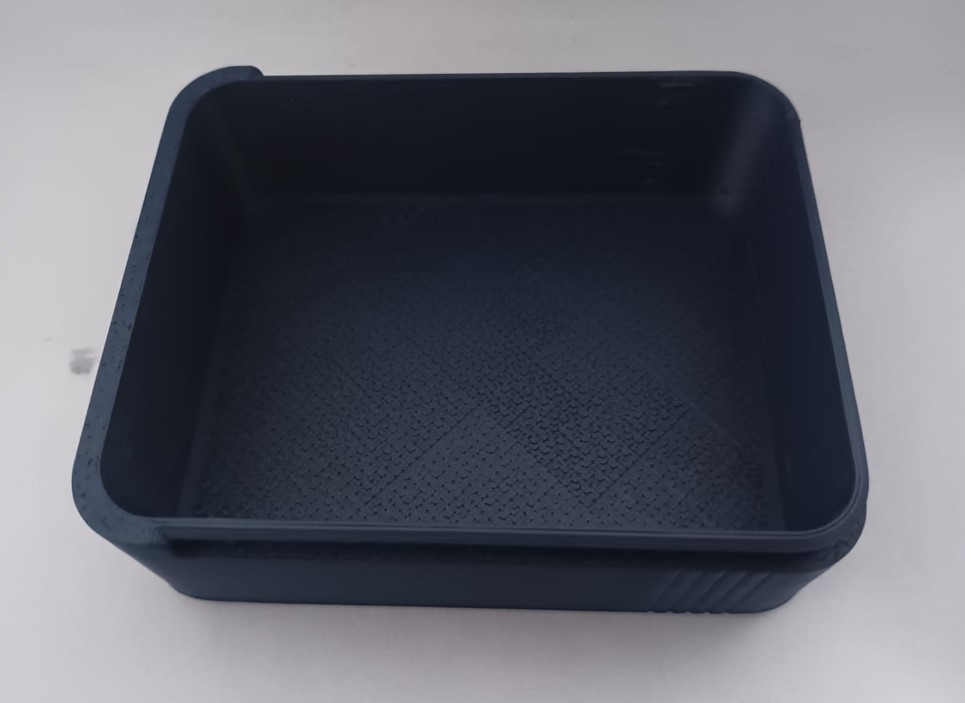
\includegraphics[width=\textwidth]{Images/CARCASA_3D.jpg}
		\caption{Base (impresa, 21~g)}
		\label{fig:carcasa_3d_base}
	\end{subfigure}
	\hfill
	\begin{subfigure}[t]{0.48\textwidth}
		\centering
		\fbox{\parbox[c][0.75\textwidth][c]{\textwidth}{\centering \textit{[Pendiente: fotografía de la tapa una vez impresa]}}}
		\caption{Tapa (pendiente, 16~g)}
		\label{fig:carcasa_3d_tapa}
	\end{subfigure}
	\vspace{2pt}
	\\
	{\footnotesize\textit{Nota.} Impresión propia en PLA. Elaboración propia.}
\end{figure}

\subsection{Diseño de la PCB (Altium Designer)}
% Tu contenido actual: monocapa, anchos de pista, bloques,
% render 3D.
Una vez concluidos los diagramas esquemáticos de cada subsistema, se procedió a la fase de diseño y distribución de la placa de circuito impreso (PCB). Para ello, se utilizó la función 'Import to PCB' integrada en Altium Designer, la cual permite transferir la conectividad lógica y las huellas físicas (footprints) de los componentes. Posteriormente, se realizó la disposición estratégica de los elementos en las diferentes capas (layers) de la placa. En la Figura \ref{fig:pcb} se ilustra detalladamente el proceso de transición de los componentes desde el entorno esquemático hacia el lienzo de diseño definitivo de la PCB. Todos estos documentos tanto como el diagrama esquematico y el layout de la PCB se muestran en el Apendice M

\begin{figure}[H]
	% Formato APA 7 con protección para el índice de figuras (Mismo estilo de tus otras figuras de EasyEDA)
	\captionsetup{labelformat=simple, labelsep=newline, textfont=it, labelfont=bf, justification=raggedright, singlelinecheck=false}
	\caption[Conversión del circuito esquemático al diseño de la PCB en Altium Designer]{Interfaz de transición y mapeo desde el diagrama esquemático hacia el entorno de diseño de la PCB.}
	\label{fig:pcb}
	\centering
	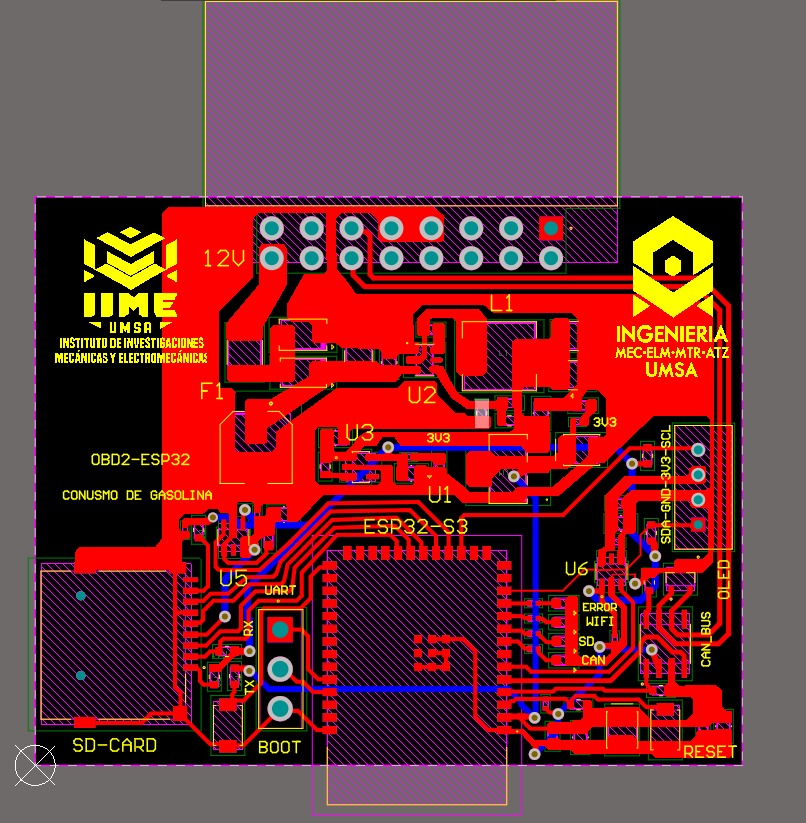
\includegraphics[width=0.85\textwidth]{Images/TRANSICION_PCB.png}
	
	\vspace{2mm}
	\small\raggedright
	\textit{Nota.} Proceso de transferencia y sincronización de componentes mediante la netlist en Altium Designer. Se ilustra cómo los símbolos lógicos del esquema eléctrico se transforman en sus respectivas huellas físicas (footprints) sobre el lienzo bidimensional de la placa de circuito impreso, quedando dispuestos para la organización de capas y el ruteado definitivo de las pistas de cobre.
\end{figure}

Previo a la fase de distribución (layout) y ruteo de las pistas de cobre, es fundamental establecer ciertos criterios técnicos de diseño. Estas consideraciones preliminares permiten optimizar la integridad de las señales, asegurar el manejo correcto de la potencia y garantizar la viabilidad de manufactura de la PCB.

\subsubsection{Criterios de integridad de señal}
% Ancho de pista por corriente (IPC-2221).
% Longitud equivalente CANH/CANL, desacople local VCC.
% Via stitching y plano de tierra (si aplica).
El diseño de circuitos impresos está regulado por estándares internacionales que garantizan su fiabilidad, rendimiento y manufacturabilidad. Entre ellos, la norma IPC-2221 (Generic Standard on Printed Board Design) constituye el pilar fundamental que establece las directrices lógicas y físicas para el desarrollo de PCB. Dentro de las buenas prácticas estipuladas por esta normativa, destacan los siguientes criterios:

\begin{itemize}
	\item \textbf{Sistemas de unidades:} Definir el sistema de medición es un paso preliminar crítico en el desarrollo de la PCB. En la práctica de la ingeniería electrónica, se prioriza el uso del sistema imperial (mils y pulgadas), debido a que el paso (pitch) y la distribución de los pines en la gran mayoría de los componentes y encapsulados comerciales están estandarizados bajo este sistema de medidas.
	
	\item \textbf{Configuración de rejillas (Grids):} La correcta gestión del grid es indispensable para garantizar la precisión geométrica, simetría y alineación del circuito. Un grid de 100~mils constituye el estándar industrial para la distribución de componentes de inserción (Through-Hole), ya que se acopla perfectamente con los centros de perforación. Para el trazo y ruteado de pistas, se adopta de forma general una rejilla de 50~mils, la cual puede reducirse a 25~mils o valores inferiores para diseños de alta densidad que requieran un nivel de detalle más fino.
	
	\item \textbf{Dimensionamiento de pistas:} El ancho de los conductores no está condicionado por un valor absoluto, sino que depende estrictamente de los requerimientos eléctricos del circuito (capacidad de corriente), el espacio disponible para el enrutamiento y las distancias de aislamiento (clearance). En la Tabla \ref{tab:pistas} se presentan los valores geométricos sugeridos; el cálculo matemático para determinar el ancho óptimo en función de la corriente y la elevación térmica es, de por sí, complejo, así que la industria se fundamenta en ecuaciones empíricas y curvas de comportamiento no lineal que han sido recopiladas y validadas experimentalmente por organismos normativos a lo largo de décadas de pruebas de laboratorio.
	
	\begin{table}[H]
		% Formato APA 7 (Estilo homogéneo, limpio y profesional)
		\captionsetup{labelformat=simple, labelsep=newline, textfont=it, labelfont=bf, justification=raggedright, singlelinecheck=false}
		\caption{Ancho de pista recomendado y resistencia estimada en función de la corriente}
		\label{tab:pistas}
		\centering
		\begin{tabular}{cccc}
			\toprule
			\rowcolor[rgb]{0.851, 0.851, 0.851}
			\textbf{Corriente (Amp)} & \textbf{1 oz (mils)} & \textbf{2 oz (mils)} & \textbf{Resistencia (m$\Omega$/plg)} \\
			\midrule
			1  & 10  & 5   & 52,0 \\
			2  & 30  & 15  & 17,2 \\
			3  & 50  & 25  & 10,3 \\
			4  & 80  & 40  & 6,4  \\
			5  & 110 & 55  & 4,7  \\
			6  & 150 & 75  & 3,4  \\
			7  & 180 & 90  & 2,9  \\
			8  & 220 & 110 & 2,3  \\
			9  & 260 & 130 & 2,0  \\
			10 & 300 & 150 & 1,7  \\
			\bottomrule
		\end{tabular}
		
		\vspace{2mm}
		\small\raggedright
		\textit{Nota.} Parámetros de diseño electrónico sugeridos para el ruteado de pistas de potencia en la PCB. Los anchos están calculados en milésimas de pulgada (mils) para los dos espesores de cobre más comunes (1~oz y 2~oz), considerando una elevación de temperatura admisible estándar ($\Delta T = 10^{\circ}\text{C}$) bajo criterios normativos de diseño industrial.
	\end{table}
	
	\item \textbf{Pads:} La geometría, dimensiones y morfología de los pads (islas de soldadura) no se determinan únicamente en función del componente seleccionado; existe un marco normativo y teórico riguroso que rige su diseño para diferentes aplicaciones electrónicas. Aunque cada fabricante de PCB (fab house) establece sus propias tolerancias y capacidades tecnológicas mínimas, una regla empírica ampliamente aceptada en la industria dicta que el diámetro del pad debe ser al menos 1{,}8 veces el diámetro de la perforación, o bien, presentar un excedente dimensional mínimo de 0{,}5 mm.
	
	\item \textbf{Vías:} Las vías constituyen las interconexiones eléctricas verticales que permiten comunicar pistas conductoras ubicadas en diferentes capas (layers) de la PCB a través de perforaciones metalizadas. En la industria del prototipado comercial (inclusive en servicios de bajo costo), esta continuidad se logra mediante un proceso de chapado electrolítico, técnicamente denominado PTH (Plated Through Hole). A diferencia de los métodos de fabricación puramente artesanales (donde se recurre a puentes de alambre o remaches mecánicos), este metalizado químico garantiza una unión uniforme, robusta y de baja resistencia eléctrica dentro de la perforación.
	
	\item \textbf{Distancias de aislamiento (Clearance):} El clearance representa un parámetro crítico y mandatorio en el diseño de cualquier PCB. Para un diseño estándar seguro, se recomienda adoptar un valor umbral de 15~mils; si bien es técnicamente viable reducir este margen a 8 o 10~mils, el diseño se encuadra en tecnologías de alta densidad (HDI), lo que exige procesos de fabricación más estrictos y costosos una referencia es la siguiente Tabla \ref{tab:clear}.
	
	\begin{table}[H]
		% Formato APA 7 (Estilo homogéneo, sin líneas verticales y con tipografía reglamentaria)
		\captionsetup{labelformat=simple, labelsep=newline, textfont=it, labelfont=bf, justification=raggedright, singlelinecheck=false}
		\caption{Distancias mínimas de aislamiento eléctrico (clearance) según el voltaje operativo y la altitud}
		\label{tab:clear}
		\centering
		\begin{tabular}{cccc}
			\toprule
			\rowcolor[rgb]{0.851, 0.851, 0.851}
			\textbf{Voltaje} & \textbf{Capas} & \textbf{Capa Externa} & \textbf{Capa Externa} \\
			\rowcolor[rgb]{0.851, 0.851, 0.851}
			\textbf{(DC o pico AC)} & \textbf{Interiores} & \textbf{($<$ 3050 m s.n.m.)} & \textbf{($>$ 3050 m s.n.m.)} \\
			\midrule
			0--15 V    & 0{,}05 mm & 0{,}10 mm & 0{,}10 mm \\
			16--30 V   & 0{,}05 mm & 0{,}10 mm & 0{,}10 mm \\
			31--50 V   & 0{,}10 mm & 0{,}60 mm & 0{,}60 mm \\
			51--100 V  & 0{,}10 mm & 0{,}60 mm & 1{,}50 mm \\
			101--150 V & 0{,}20 mm & 0{,}60 mm & 3{,}20 mm \\
			151--170 V & 0{,}20 mm & 1{,}25 mm & 3{,}20 mm \\
			171--250 V & 0{,}20 mm & 1{,}25 mm & 6{,}40 mm \\
			251--300 V & 0{,}20 mm & 1{,}25 mm & 12{,}50 mm \\
			301--500 V & 0{,}25 mm & 2{,}50 mm & 12{,}50 mm \\
			\bottomrule
		\end{tabular}
		
		\vspace{2mm}
		\small\raggedright
		\textit{Nota.} Directrices de espaciamiento mínimo (clearance) adaptadas de la norma IPC-2221B \citep{IPC2221B2012}. 
	\end{table}
	
	\item \textbf{Constante dieléctrica:} Entre los parámetros más importantes en los 
	PCB está también la constante dieléctrica, 	usada para cálculos de parámetros en líneas de alta velocidad como referencia se tiene la Tabla \ref{tab:dielectrica}.
	
	\begin{table}[H]
		% Formato APA 7 (Estilo limpio, sin líneas verticales y alineación reglamentaria)
		\captionsetup{labelformat=simple, labelsep=newline, textfont=it, labelfont=bf, justification=raggedright, singlelinecheck=false}
		\caption{Constante dieléctrica relativa de materiales comunes en sustratos de PCB}
		\label{tab:dielectrica}
		\centering
		\begin{tabular}{lc}
			\toprule
			\rowcolor[rgb]{0.851, 0.851, 0.851}
			\textbf{Material} & \textbf{Constante Dieléctrica ($\varepsilon_r$)} \\
			\midrule
			FR4    & 3{,}8 -- 4{,}8 \\
			FR5    & 4{,}2 \\
			Vidrio & 6{,}0 \\
			Resina & 3{,}0 \\
			\bottomrule
		\end{tabular}
		
		\vspace{2mm}
		\small\raggedright
		\textit{Nota.} Valores típicos de la permitividad eléctrica relativa ($\varepsilon_r$) evaluados a frecuencias estándar de operación.
	\end{table}
	
\end{itemize}

% =====================================================================
%  SECCIÓN: PARÁMETROS DE DISEÑO DEL PCB (IPC-2221B), BOM Y JLCPCB
%  Tesis: Sistema de monitoreo de consumo de combustible OBD-II / CAN
%
%  PAQUETES REQUERIDOS (verificar que estén en el preámbulo principal):
%     \usepackage{amsmath}      % ecuaciones
%     \usepackage{booktabs}     % \toprule, \midrule, \bottomrule
%     \usepackage{float}        % opción [H] para fijar tablas/figuras
%     \usepackage{graphicx}     % \includegraphics
%     \usepackage{array}        % columnas p{} con texto envuelto
%     \usepackage{longtable}    % (solo si el BOM se extiende a >1 página)
%
%  CONVENCIÓN APA 7 USADA: número y título de tabla/figura ARRIBA;
%  "Nota." en \footnotesize\textit{} ABAJO. Citas con natbib (\citep/\citet).
%
%  FIGURAS: se dejan marcadores \includegraphics con un comentario que
%  describe qué debe mostrar cada una; reemplazar la ruta por tu imagen.
% =====================================================================

\subsection{Parámetros de diseño del PCB según la norma IPC-2221B}

Después de revisar estos conceptos y ser validados con la norma IPC-2221B
\citep{IPC2221B2012}, se definieron los criterios de diseño que permiten obtener
un PCB conforme a dicho estándar. La IPC-2221B constituye el documento genérico
de referencia para el diseño de placas de circuito impreso de una, dos o más
capas, y establece, entre otros aspectos, los requisitos de ancho de pista,
separación entre conductores (\textit{clearance}), distancias de fuga
(\textit{creepage}) y dimensiones de vías \citep{IPC2221B2012}. 

Con estos criterios claros, los parámetros adoptados para la fabricación de la placa de
dos capas (35~\textmu m de cobre, 1~oz) se resumen en la
Tabla~\ref{parametros_pcb}. A continuación se justifica cada grupo de valores a
partir del estándar, de las capacidades del fabricante \citep{JLCPCB2025} y de
las corrientes reales estimadas en el presupuesto de potencia del sistema.

\subsubsection{Ancho de pistas (capacidad de corriente)}

El ancho mínimo de una pista se determina por la corriente que debe conducir y
por el incremento de temperatura admisible debido al efecto Joule. La IPC-2221B
deriva el área transversal de cobre necesaria a partir de la Ecuación
\ref{eq:ancho_pista}, donde la corriente, el sobrecalentamiento y un coeficiente
ligado a la ubicación de la pista (externa o interna) fijan la sección de cobre
requerida \citep{IPC2221B2012}. 

Para diseños de alta exactitud en capacidad de
corriente, el estándar moderno IPC-2152 reemplaza a estas curvas históricas;
sin embargo, la formulación de la IPC-2221B sigue siendo válida y conservadora
para placas de baja potencia como la presente \citep{IPC2152_2009}.

\begin{equation}
	A = \left( \frac{I}{k \cdot \Delta T^{\,0{,}44}} \right)^{\!1/0{,}725}
	\label{eq:ancho_pista}
\end{equation}

\noindent donde:

\begin{center}
	\begin{tabular}{r l}
		$A$        & : área transversal de la pista [mils$^2$] \\
		$I$        & : corriente que circula por la pista [A] \\
		$\Delta T$ & : incremento de temperatura admisible sobre el ambiente [$^\circ$C] \\
		$k$        & : constante ($k=0{,}048$ para pistas externas; $k=0{,}024$ internas) \\
	\end{tabular}
\end{center}

\noindent A partir del área obtenida, el ancho de la pista se calcula con la
Ecuación \ref{eq:ancho_w}, considerando el espesor de cobre de 1~oz
($t = 35$~\textmu m $= 1{,}378$~mils):

\begin{equation}
	W = \frac{A}{t}
	\label{eq:ancho_w}
\end{equation}

Para la línea de mayor consumo del sistema (el riel de 3,3~V, que alimenta de
forma conjunta al ESP32-S3-WROOM-1-N16R8, el transceptor CAN, la tarjeta MicroSD y la
pantalla OLED), el presupuesto de potencia arrojó una corriente pico de
aproximadamente $0{,}76$~A. Diseñando con un margen de seguridad hasta
$I = 1$~A, un sobrecalentamiento conservador de $\Delta T = 10\,^\circ$C y
$k = 0{,}048$ (pista externa), la Ecuación \ref{eq:ancho_pista} entrega
$A \approx 16{,}3$~mils$^2$, que con la Ecuación \ref{eq:ancho_w} corresponde a
un ancho mínimo de $W \approx 11{,}8$~mils $\approx 0{,}30$~mm. En otras
palabras, $0{,}30$~mm bastarían para 1~A; no obstante, se adoptó un ancho de
\textbf{1,0~mm} para las pistas de potencia (entrada de 12~V y riel de 3,3~V).

Esta decisión, holgada respecto al mínimo, responde a tres criterios de diseño:
(i) reducir la caída de tensión $IR$ y la resistencia serie del riel, evitando
caídas que afecten la regulación de 3,3~V; (ii) disminuir la elevación de
temperatura para mejorar la fiabilidad térmica, dado que un ancho de $1{,}0$~mm
en cobre de 1~oz admite del orden de $2{,}4$~A con el mismo $\Delta T = 10\,^\circ$C
(más de tres veces la corriente pico real); y (iii) ofrecer una vía de retorno
de baja impedancia que mitiga el ruido del regulador conmutado. Para las pistas
de señal de baja corriente (GPIO, I\textsuperscript{2}C, SPI de la MicroSD) se
adoptó $0{,}20$~mm, ancho gobernado por la densidad de ruteo y el límite de
fabricación (no por la corriente, ya que estas líneas conducen apenas algunos
miliamperios), y se mantiene por encima del mínimo de $0{,}127$~mm del fabricante
\citep{JLCPCB2025}. Finalmente, el par diferencial del bus CAN (CANH/CANL) se
ruteó con pistas de $0{,}30$~mm, acopladas y de igual longitud; a 500~kbps y
sobre trazos cortos la impedancia diferencial nominal de 120~$\Omega$ no es
crítica, por lo que prima el apareamiento geométrico y de longitud del par sobre
el control estricto de impedancia.

\subsubsection{Separación entre conductores (\textit{clearance})}

La separación mínima entre conductores se establece a partir de la tensión de
trabajo pico entre ellos, según la Tabla 6-1 de la IPC-2221B
\citep{IPC2221B2012}. El riel de mayor tensión del diseño es la entrada de 12~V
proveniente del conector OBD-II; aun considerando transitorios del sistema
eléctrico automotriz, la tensión de trabajo se mantiene por debajo de 30~V. La
Tabla~\ref{clearance_ipc} reproduce los valores relevantes del estándar para
conductores externos sin recubrimiento.

% --------------------- Tabla: clearance IPC-2221B ---------------------
\begin{table}[H]
	% Formato APA 7 (Estilo limpio, sin líneas verticales y alineación reglamentaria)
	\captionsetup{labelformat=simple, labelsep=newline, textfont=it, labelfont=bf, justification=raggedright, singlelinecheck=false}
	\caption{Separación mínima entre conductores externos sin recubrimiento (IPC-2221B, Tabla 6-1)}
	\label{clearance_ipc}
	\centering
	\begin{tabular}{c c c}
		\toprule
		\rowcolor[rgb]{0.851, 0.851, 0.851}
		\textbf{Tensión pico} & \textbf{Hasta 3050 m (B1)} & \textbf{Sobre 3050 m (B2)} \\
		$[$V$]$ & $[$mm$]$ & $[$mm$]$ \\
		\midrule
		$\leq 15$  & 0,10 & 0,10 \\
		$\leq 30$  & 0,10 & 0,10 \\
		$\leq 50$  & 0,60 & 0,60 \\
		$\leq 100$ & 0,60 & 1,50 \\
		$\leq 150$ & 0,60 & 3,20 \\
		\bottomrule
	\end{tabular}
	
	\vspace{2pt}
	{\footnotesize\textit{Nota.} Valores derivados de la Tabla 6-1 de la norma IPC-2221B
		\citep{IPC2221B2012}. La columna B1 corresponde a conductores externos sin
		recubrimiento desde el nivel del mar hasta 3050~m; la columna B2, a la misma
		condición por encima de 3050~m.}
\end{table}

Un aspecto particular de este proyecto es la altitud de La Paz
($\approx 3600$~m s.\,n.\,m.), superior al umbral de 3050~m que separa las
categorías B1 y B2 de la norma. Dado que la reducción de presión atmosférica
disminuye la rigidez dieléctrica del aire (ley de Paschen), la IPC-2221B exige
mayores separaciones por encima de 3050~m. Sin embargo, como se observa en la
Tabla~\ref{clearance_ipc}, para tensiones de trabajo $\leq 30$~V (rango en el
que opera la totalidad de este diseño) el valor exigido es idéntico en ambas
categorías ($0{,}10$~mm): el penalti por altitud solo se vuelve significativo a
partir de $\sim 100$~V (por ejemplo, $0{,}60$~mm frente a $1{,}50$~mm). Por
tanto, se concluye que la altitud de La Paz no impone requisitos
	adicionales de separación para esta placa de baja tensión, aunque sí es un
factor determinante en el modelo de cálculo de consumo de combustible por su
efecto sobre la densidad del aire.

Sobre esta base, y siempre por encima del mínimo del fabricante de $0{,}127$~mm
\citep{JLCPCB2025}, se adoptaron separaciones conservadoras: $0{,}20$~mm como
\textit{clearance} general de señal y $0{,}50$~mm en la sección de entrada de
12~V, esta última para absorber con holgura eventuales sobretensiones del bus de
12~V del vehículo y facilitar el ensamblaje. Todos los conductores se mantienen
además a $\geq 0{,}30$~mm del borde de la placa, según la capacidad del
fabricante \citep{JLCPCB2025}.

Una vez establecidos estos criterios y reglas de diseño, se procedió con su implementación en el software Altium Designer. Como resultado, se consolidó el esquemático completo del circuito y el ruteado de la placa de circuito impreso (PCB), garantizando la correcta disposición de vías y distancias de separación (clearance) bajo los lineamientos de la norma IPC. El esquemático eléctrico completo, la disposición de capas y el ruteado de la PCB, y el reporte de la pila de capas se presentan en el Apéndice~M.
% --------------------- Tabla CONSOLIDADA de parámetros ---------------------
\begin{table}[H]
	\captionsetup{labelformat=simple, labelsep=newline, textfont=it, labelfont=bf, justification=raggedright, singlelinecheck=false}
	\caption{Parámetros de diseño del PCB conforme a IPC-2221B y capacidades de JLCPCB}
	\label{parametros_pcb}
	\centering
	\begin{tabular}{p{5.0cm} c p{5.0cm}}
		\toprule
		\rowcolor[rgb]{0.851, 0.851, 0.851}
		\textbf{Parámetro} & \textbf{Valor adoptado} & \textbf{Criterio / Referencia} \\
		\midrule
		Ancho de pistas de potencia (12~V, 3,3~V) & 1,00 mm & Margen $\approx 3\times$ sobre 0,76~A pico; baja caída $IR$ \citep{IPC2221B2012} \\[2pt]
		Ancho de pistas de señal (GPIO, I\textsuperscript{2}C, SPI) & 0,20 mm & Densidad de ruteo; $>$ mínimo de fábrica \citep{JLCPCB2025} \\[2pt]
		Ancho del par diferencial CAN (CANH/CANL) & 0,30 mm & Par acoplado y apareado en longitud \\[2pt]
		Separación general de señal & 0,20 mm & $>$ mínimo IPC y de fábrica \citep{IPC2221B2012,JLCPCB2025} \\[2pt]
		Separación en sección de 12~V & 0,50 mm & Margen ante transitorios automotrices \\[2pt]
		Separación mínima absoluta (fábrica) & 0,127 mm & Límite 2 capas, 1~oz \citep{JLCPCB2025} \\[2pt]
		Diámetro de perforación de vía & 0,30 mm & Vía estándar fiable \citep{JLCPCB2025} \\[2pt]
		Diámetro de \textit{pad} de vía & 0,60 mm & Anillo anular $0{,}15$~mm \citep{JLCPCB2025} \\[2pt]
		Anillo anular mínimo & 0,15 mm & Capacidad de fábrica \citep{JLCPCB2025} \\[2pt]
		Distancia cobre--borde de placa & 0,30 mm & Capacidad de fábrica \citep{JLCPCB2025} \\[2pt]
		Espesor de cobre & 1 oz (35~\textmu m) & Estándar de uso general \citep{JLCPCB2025} \\[2pt]
		Espesor de placa & 1,60 mm & FR-4 estándar \\[2pt]
		Acabado superficial & HASL sin plomo & Estándar de bajo costo \citep{JLCPCB2025} \\[2pt]
		Dimensiones del PCB & 40~$\times$~60 mm & Restricción mecánica del encapsulado OBD-II \\
		\bottomrule
	\end{tabular}
	
	\vspace{2pt}
	{\footnotesize\textit{Nota.} Parámetros validados contra la norma IPC-2221B
		\citep{IPC2221B2012} y las capacidades de fabricación de JLCPCB
		\citep{JLCPCB2025}. Los anchos de pista se verificaron con la
		Ecuación \ref{eq:ancho_pista} para la corriente pico estimada del sistema.}
\end{table}

% --------------------- FIGURA (marcador) ---------------------

% layout, los tres anchos de pista (1,0 / 0,2 / 0,3 mm) y las separaciones
% (0,2 / 0,5 mm). Una captura del DRC de EasyEDA con las reglas activas también
% sirve. Reemplaza la ruta del \includegraphics por tu imagen.
\begin{figure}[H]
	\centering
	\caption{Anchos de pista en el ruteo del PCB}
	\label{fig:pistas_clearance}
	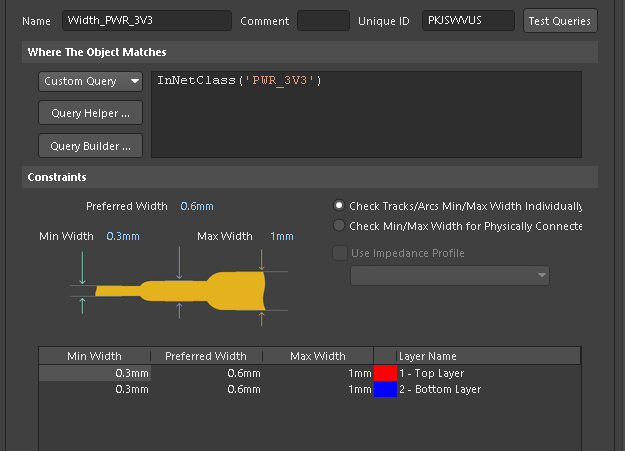
\includegraphics[width=1.05\textwidth]{Images/1.png}
%	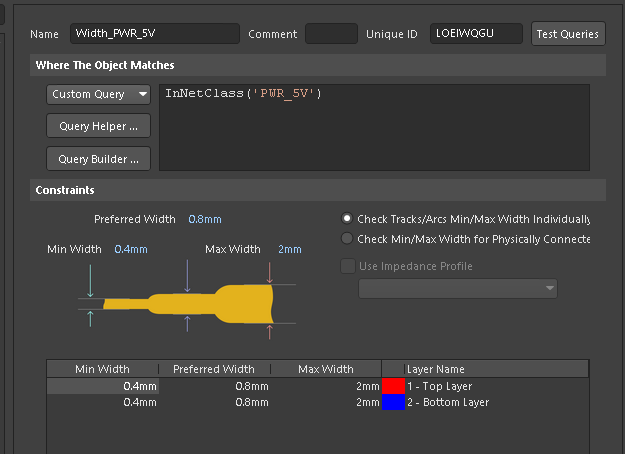
\includegraphics[width=0.75\textwidth]{Images/2.png}
%	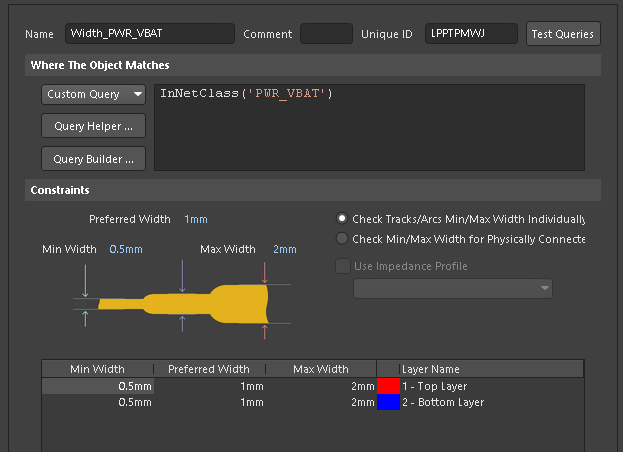
\includegraphics[width=0.75\textwidth]{Images/3.png}
	\vspace{2pt}\\
	{\footnotesize\textit{Nota.} Elaboración propia a partir del diseño en Altium Designer.}
\end{figure}

% =====================================================================
\subsection{Lista de materiales (BOM)}

La lista de materiales (\textit{Bill of Materials}, BOM) consolida todos los
componentes del dispositivo, organizados por bloque funcional: etapa de
alimentación de dos rieles basada en el convertidor reductor síncrono
TPS54302DDCR (12~V~$\rightarrow$~5~V) seguido de los reguladores lineales
AMS1117-3.3 y AP2112K-3.3TRG1 (5~V~$\rightarrow$~3,3~V), unidad de
procesamiento ESP32-S3-WROOM-1-N16R8 \citep{espressif_esp32_datasheet},
interfaz de bus CAN con el transceptor SN65HVD230
\citep{sn65hvd230_datasheet}, almacenamiento en MicroSD, interfaz de usuario
OLED y conector OBD-II. Los valores de los componentes pasivos de la etapa de
potencia se seleccionaron siguiendo el procedimiento de diseño y el
esquemático típico de aplicación del fabricante del regulador, detallado en
la subsección anterior. La Tabla~\ref{bom} presenta un resumen; el detalle de
fabricación (huellas, designadores agrupados y códigos de parte LCSC) se
presenta en el Apéndice~N.

% --------------------- Tabla BOM ---------------------
\begingroup
\captionsetup{labelformat=simple, labelsep=newline, textfont=it, labelfont=bf, justification=raggedright, singlelinecheck=false}
\small
\begin{longtable}{c p{5.9cm} p{3.0cm} c c}
	\caption{Lista de materiales (BOM) del dispositivo}
	\label{bom} \\
	\toprule
	\rowcolor[rgb]{0.851, 0.851, 0.851}
	\textbf{Ref.} & \textbf{Componente} & \textbf{Valor / Parte} & \textbf{Encap.} & \textbf{Cant.} \\
	\midrule
	\endfirsthead
	\multicolumn{5}{l}{\textit{Tabla~\ref{bom} (continuación)}} \\
	\toprule
	\rowcolor[rgb]{0.851, 0.851, 0.851}
	\textbf{Ref.} & \textbf{Componente} & \textbf{Valor / Parte} & \textbf{Encap.} & \textbf{Cant.} \\
	\midrule
	\endhead
	\midrule
	\multicolumn{5}{r}{\textit{Continúa en la siguiente página\ldots}} \\
	\endfoot
	\bottomrule
	\endlastfoot
		\multicolumn{5}{l}{\textit{Etapa de alimentación, riel 1 de 2 (12~V $\rightarrow$ 5~V, síncrona)}} \\
		U1 & Convertidor reductor (buck) síncrono & TPS54302DDCR & SOT-23-6 & 1 \\
		L1 & Inductor de potencia          & 10~\textmu H      & SMD    & 1 \\
		D2 & Diodo protección polaridad inv.& SS34 (3~A/40~V)  & SMA    & 1 \\
		F1 & Fusible reseteable PTC        & $I_{hold}\approx 1{,}5$~A & 1812 & 1 \\
		C1,C2 & Condensador de entrada     & 4,7~\textmu F / 50~V X7R & 1206 & 2 \\
		C3 & Condensador de entrada (HF)   & 0,01~\textmu F    & 0603 & 1 \\
		C4,C5 & Condensador de salida (44~\textmu F efectivos) & 22~\textmu F / 16~V X5R & 1206 & 2 \\
		C6 & Condensador de mejora transitoria & 75~pF         & 0603 & 1 \\
		R1 & Resistor divisor realim. (sup.) & 100~k$\Omega$   & 0603 & 1 \\
		R2 & Resistor divisor realim. (inf.) & 13,3~k$\Omega$  & 0603 & 1 \\
		\midrule
		\multicolumn{5}{l}{\textit{Etapa de alimentación, riel 2 de 2 (5~V $\rightarrow$ 3,3~V, dos rieles LDO)}} \\
		U4 & LDO riel 1 (ESP32-S3, hasta 1~A), siempre activo & AMS1117-3.3 & SOT-223 & 1 \\
		U5 & LDO riel 2 (periféricos, hasta 600~mA) & AP2112K-3.3TRG1 & SOT-23-5 & 1 \\
		C14,C15 & Desacople entrada/salida AMS1117 & 10~\textmu F & 1206 & 2 \\
		C16,C17 & Desacople entrada/salida AP2112 & 1~\textmu F & 0603 & 2 \\
		\midrule
		\multicolumn{5}{l}{\textit{Unidad de procesamiento}} \\
		U2 & Microcontrolador (módulo)     & ESP32-S3-WROOM-1-N16R8 & Módulo & 1 \\
		R3 & \textit{Pull-up} EN           & 10~k$\Omega$      & 0603 & 1 \\
		C7 & Condensador EN                & 0,1~\textmu F     & 0603 & 1 \\
		C8--C11 & Desacople de alimentación & 0,1~\textmu F    & 0603 & 4 \\
		C12 & Reserva de carga (\textit{bulk}) 3,3~V & 10~\textmu F & 0805 & 1 \\
		SW1 & Pulsador de \textit{reset}   & ---               & SMD  & 1 \\
		SW2 & Pulsador BOOT (GPIO0)        & ---               & SMD  & 1 \\
		\midrule
		\multicolumn{5}{l}{\textit{Interfaz de bus CAN}} \\
		U3 & Transceptor CAN               & SN65HVD230        & SOIC-8 & 1 \\
		R4 & Resistor de control de pendiente  & 10~k$\Omega$ & 0603 & 1 \\
		R5 & Resistor de terminación (opcional)$^{a}$ & 120~$\Omega$ & 0805 & 1 \\
		C13 & Desacople                    & 0,1~\textmu F     & 0603 & 1 \\
		\midrule
		\multicolumn{5}{l}{\textit{Almacenamiento y pantalla}} \\
		J2 & Zócalo MicroSD (push-push)    & ---               & SMD  & 1 \\
		R6--R9 & \textit{Pull-up} líneas SPI & 10~k$\Omega$    & 0603 & 4 \\
		DISP1 & Pantalla OLED I\textsuperscript{2}C 0,96" & SSD1306 & Módulo & 1 \\
		R10,R11 & \textit{Pull-up} I\textsuperscript{2}C (SDA/SCL) & 4,7~k$\Omega$ & 0603 & 2 \\
		\midrule
		\multicolumn{5}{l}{\textit{Conectores e indicadores}} \\
		J1 & Conector OBD-II (12~V, GND, CANH, CANL) & 4 pines & --- & 1 \\
		LED1 & LED indicador de alimentación & Verde           & 0805 & 1 \\
		LED2 & LED indicador de estado      & Azul             & 0805 & 1 \\
		R12,R13 & Resistor limitador de LED & 1~k$\Omega$       & 0805 & 2 \\
\end{longtable}
\endgroup

\vspace{2pt}
{\footnotesize\textit{Nota.} Elaboración propia. Los valores de la etapa de
	alimentación siguen el procedimiento de diseño del fabricante para el
	TPS54302DDCR, detallado en la subsección de diseño de hardware de este
	capítulo. $^{a}$El resistor de terminación de 120~$\Omega$ se
	deja como \textit{footprint} opcional (no poblado por defecto), dado que el
	dispositivo se conecta como nodo en derivación a un bus CAN que ya posee sus
	terminaciones en el vehículo.}

% =====================================================================
\subsection{Capacidades de fabricación de JLCPCB}

El PCB se fabricó mediante el servicio de prototipado de JLCPCB, integrado de
forma nativa con la herramienta EasyEDA empleada en el diseño. Para garantizar
una producción correcta y de alto rendimiento (\textit{Right-First-Time}), las
reglas de diseño (DRC) del proyecto se ajustaron a las capacidades del
fabricante para placas de dos capas en cobre de 1~oz \citep{JLCPCB2025}. La
Tabla~\ref{jlcpcb} compara los límites de fabricación con los valores adoptados
en este diseño, evidenciando que todos los parámetros se mantienen dentro de la
ventana de proceso estándar (la más económica y de mayor rendimiento de
producción).

% --------------------- Tabla capacidades JLCPCB ---------------------
\begin{table}[H]
	
	\captionsetup{labelformat=simple, labelsep=newline, textfont=it, labelfont=bf, justification=raggedright, singlelinecheck=false}
	\caption{Capacidades de fabricación de JLCPCB (2 capas, 1~oz) frente al diseño}
	\label{jlcpcb}
	\centering
	\begin{tabular}{p{5.2cm} c c}
		\toprule
		\rowcolor[rgb]{0.851, 0.851, 0.851}
		\textbf{Parámetro de fabricación} & \textbf{Mínimo JLCPCB} & \textbf{Diseño} \\
		\midrule
		Ancho mínimo de pista        & 0,127 mm (5 mil) & 0,20 mm \\
		Separación mínima de pista   & 0,127 mm (5 mil) & 0,20 mm \\
		Diámetro mínimo de perforación & 0,20 mm        & 0,30 mm \\
		Anillo anular mínimo         & 0,15 mm          & 0,15 mm \\
		Distancia cobre--borde       & 0,30 mm          & 0,30 mm \\
		Altura mínima de texto (serigrafía) & 1,00 mm   & $\geq 1$ mm \\
		Ancho mínimo de línea (serigrafía)  & 0,15 mm   & $\geq 0{,}15$ mm \\
		Expansión de máscara antisoldante   & 0,05 mm   & 0,05 mm \\
		Espesor de cobre             & 1 oz (35~\textmu m) & 1 oz \\
		Tamaño de placa (rango)      & 5$\times$5 a 400$\times$500 mm & 40$\times$60 mm \\
		\bottomrule
	\end{tabular}
	
	\vspace{2pt}
	{\footnotesize\textit{Nota.} Capacidades según la documentación de fabricación de
		JLCPCB \citep{JLCPCB2025}. Todos los valores del diseño cumplen o superan el
		mínimo del fabricante, situándose en la categoría de proceso estándar.}
\end{table}

% --------------------- FIGURA (marcador) --------------------
%Inserta aquí una captura del reporte DFM/DRC de JLCPCB o de la
% vista previa de Gerbers (cara superior/inferior) confirmando que el diseño
% pasa la verificación de fabricación. Reemplaza la ruta del \includegraphics.
\begin{figure}[H]
	\centering
	\caption{Verificación de fabricabilidad (DFM) del PCB en JLCPCB}
	\label{fig:jlcpcb_dfm}
	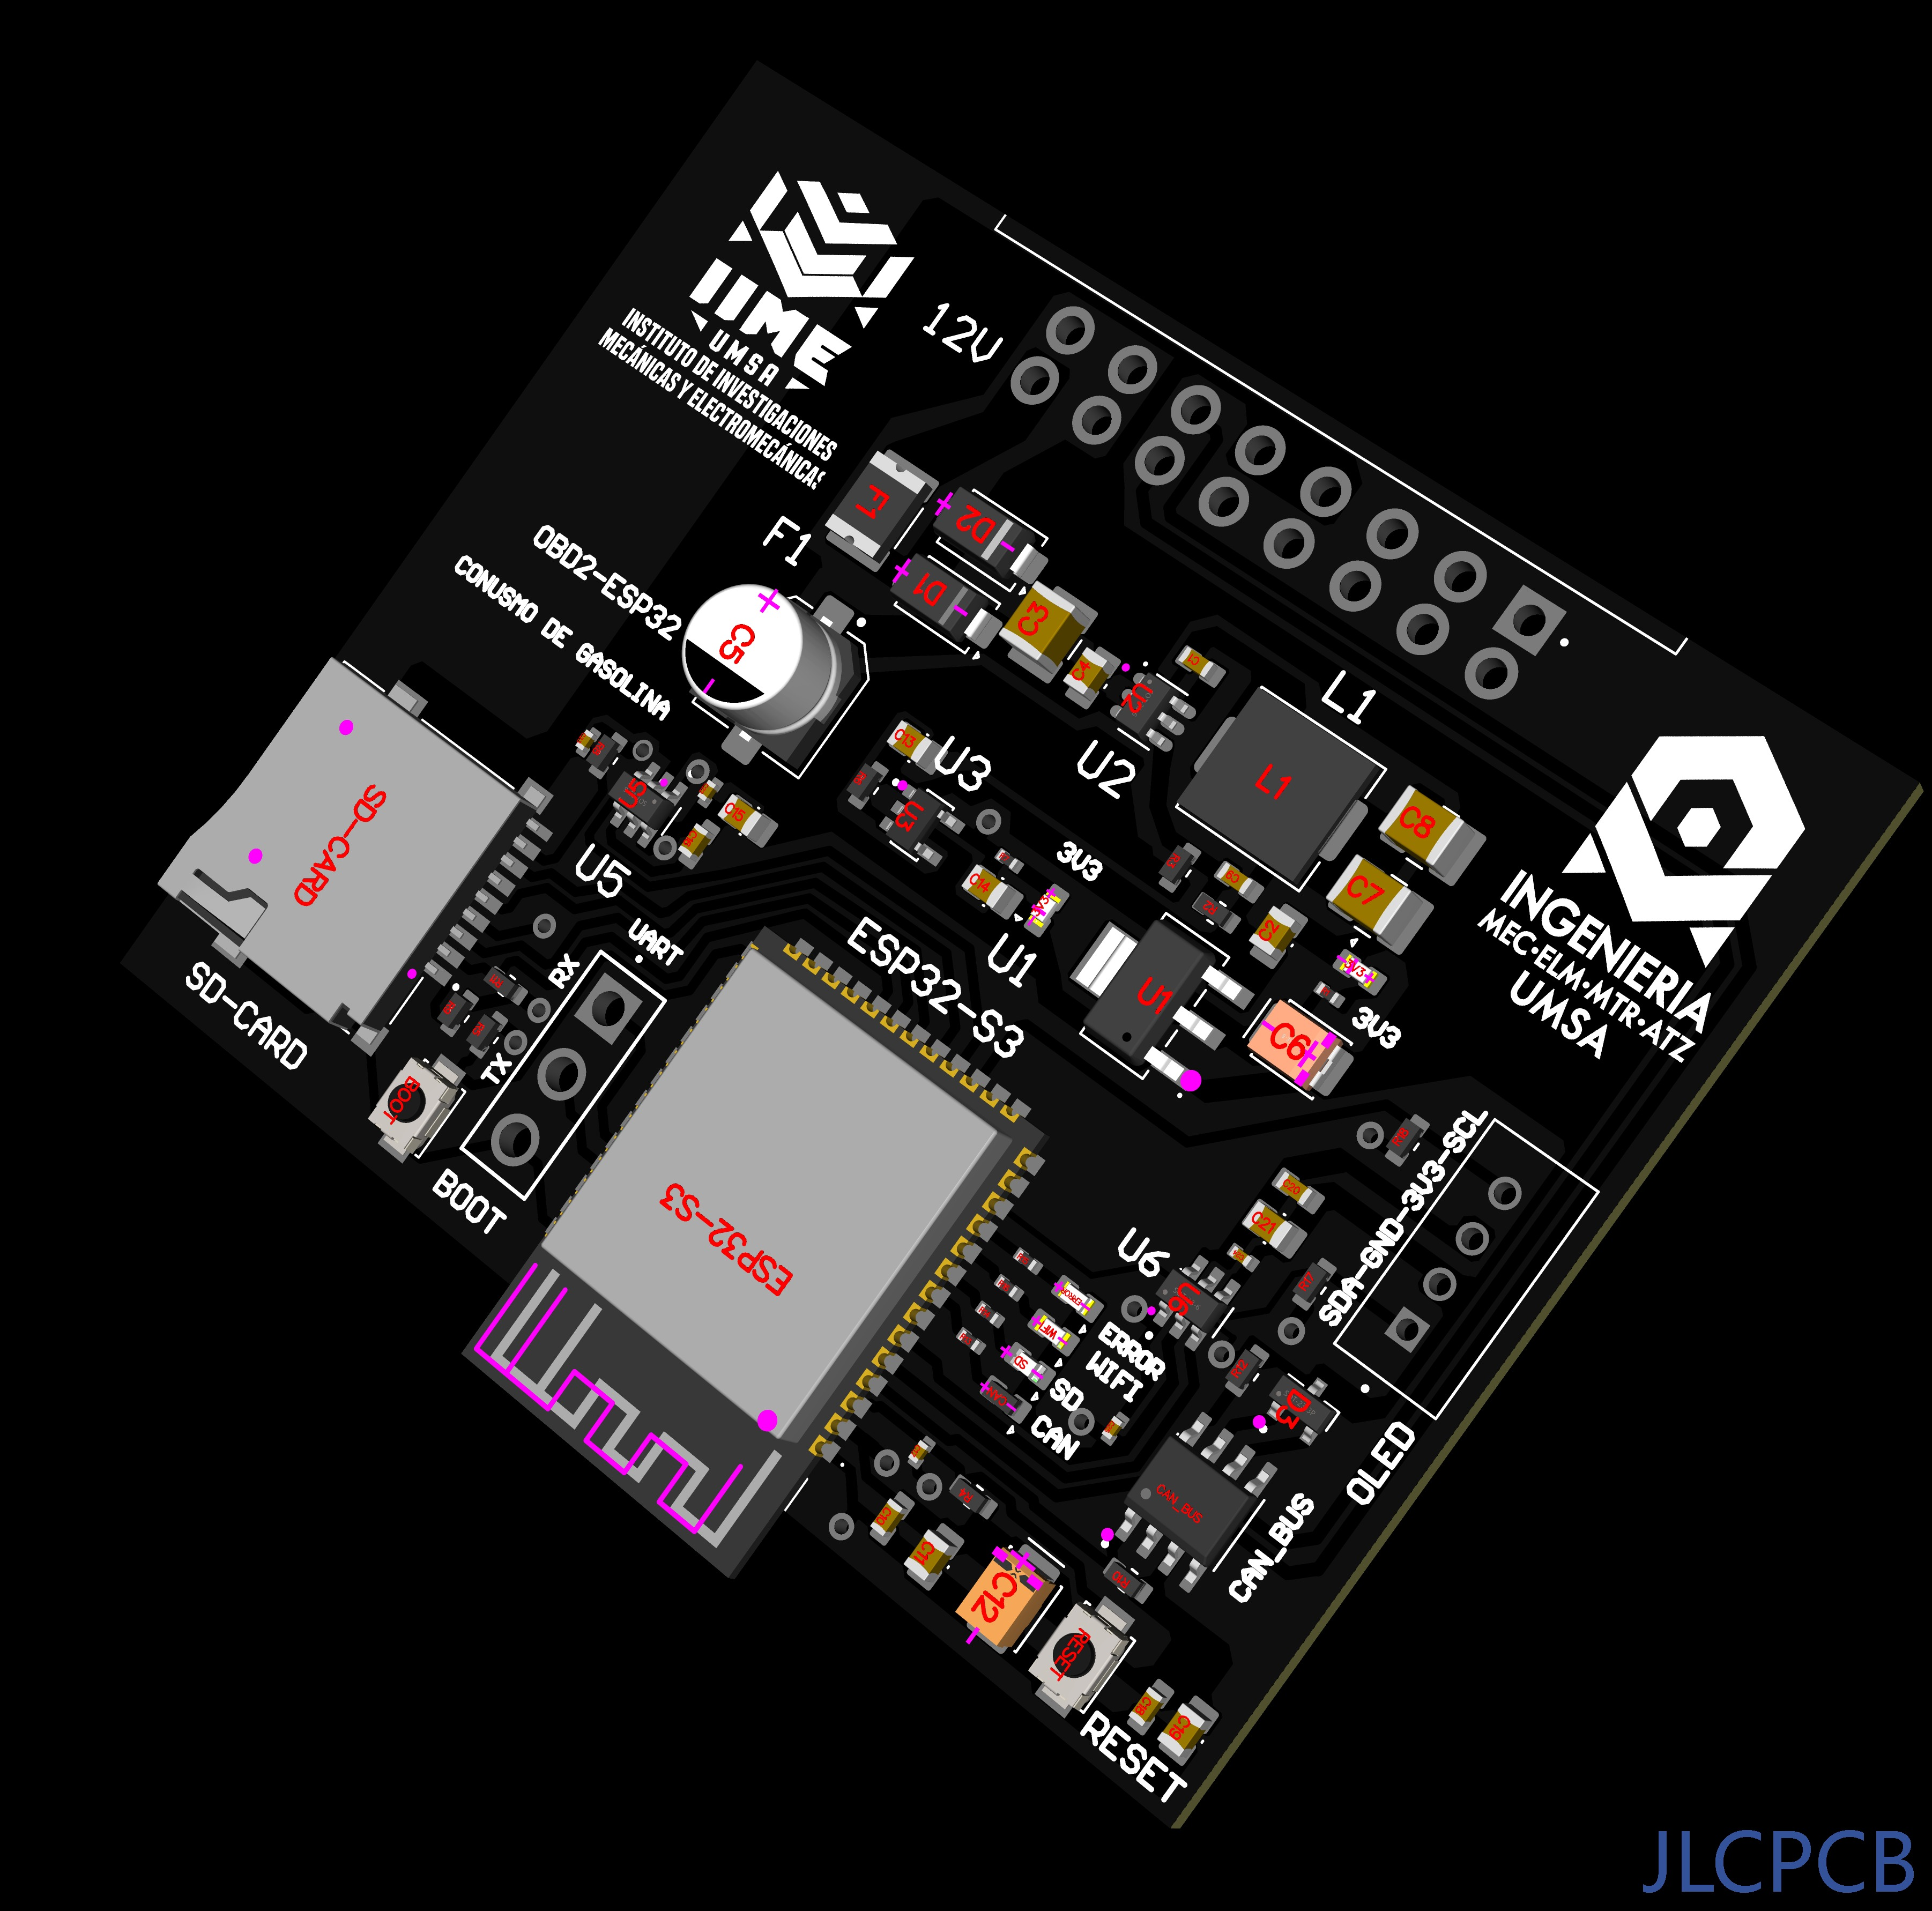
\includegraphics[width=0.8\textwidth]{Images/3D_PCB.png}
	
	\vspace{2pt}
	{\footnotesize\textit{Nota.} Captura obtenida del servicio de fabricación JLCPCB
		\citep{JLCPCB2025}.}
\end{figure}


\subsection{Diseño de la carcasa (impresión 3D)}

Aquí realizare el envase al PCB , cuando pida la PCB pondré aquí información.

% ────────────────────────────────────────────────────────────
% =====================================================================
%  SECCIÓN: MODELO MATEMÁTICO DE ESTIMACIÓN DE CONSUMO DE COMBUSTIBLE
%  Enfoque: deducción de ecuaciones desde principios físicos + criterios
%
%  PAQUETES REQUERIDOS (verificar en el preámbulo principal):
%     \usepackage{amsmath}
%     \usepackage{booktabs}
%     \usepackage{float}
%     \usepackage{graphicx}
%     \usepackage{array}
%     \usepackage[ruled,vlined,linesnumbered]{algorithm2e}  % pseudocódigo
%     \usepackage{tikz}                                      % diagrama de estados
%     \usetikzlibrary{shapes.geometric,arrows.meta,positioning}
%     \usepackage{natbib}                                    % citas APA 7
%
%  CONVENCIÓN APA 7: número/título de tabla y figura ARRIBA; "Nota." abajo.
% =====================================================================

\section{Modelo matemático de estimación de consumo de combustible}

En la sección 2.7 se desarrolló el marco teórico de los modelos de estimación de
consumo de combustible. En este apartado, en cambio, se deducen y formalizan las
ecuaciones que se implementarán directamente en el software del dispositivo,
partiendo de principios físicos (conservación de masa, ley de los gases ideales
y relación aire-combustible) y aplicando los criterios de ingeniería que rigen la
selección de variables, parámetros y fuentes de datos (PIDs OBD-II). El objetivo
es obtener un conjunto de expresiones cerradas, computables en tiempo real sobre
el ESP32, junto con conclusiones operativas sobre qué PIDs deben consultarse y
con qué prioridad.

% =====================================================================
\subsection{Método por sensor MAF}

El método más directo parte de la medición del flujo másico de aire admitido por
el motor, $\dot{m}_{air}$ [g/s], reportado por el sensor MAF (\textit{Mass Air
	Flow}) a través del PID 0x10 \citep{sae_j1979_2014}. La estimación de combustible
se fundamenta en la relación aire-combustible (\textit{Air-Fuel Ratio}, AFR),
definida como el cociente entre la masa de aire y la masa de combustible de la
mezcla \citep{Heywood2018}:

\begin{equation}
	\mathrm{AFR} = \frac{\dot{m}_{air}}{\dot{m}_{fuel}}
	\label{eq:afr}
\end{equation}

Para la gasolina, la relación estequiométrica es $\mathrm{AFR}_{s} \approx 14{,}7$
(14,7 kg de aire por cada kg de combustible) \citep{Heywood2018, Bosch2014}. La
mezcla real rara vez es exactamente estequiométrica; la ECU la regula en torno a
$\lambda = 1$, donde $\lambda$ es el factor lambda (relación de equivalencia
inversa) disponible en el PID 0x44. La relación real se expresa entonces como
$\mathrm{AFR} = \lambda \cdot \mathrm{AFR}_{s}$, y despejando $\dot{m}_{fuel}$ de
la Ecuación \ref{eq:afr} se obtiene el flujo másico de combustible:

\begin{equation}
	\dot{m}_{fuel} = \frac{\dot{m}_{air}}{\lambda \cdot \mathrm{AFR}_{s}}
	\label{eq:mfuel}
\end{equation}

El flujo másico se convierte a flujo volumétrico dividiendo por la densidad del
combustible, $\rho_{fuel} \approx 745$~kg/m$^3$ para la gasolina
\citep{Bosch2014}. Considerando que $1$~kg/m$^3 = 1$~g/L y que $\dot{m}_{air}$ se
expresa en g/s, el caudal de combustible en litros por hora (FuelRate) resulta de
incorporar el factor de conversión temporal $3600$~s/h:

\begin{equation}
	\mathrm{FuelRate}\;[\mathrm{L/h}]
	= \frac{3600 \cdot \dot{m}_{air}}{\lambda \cdot \mathrm{AFR}_{s} \cdot \rho_{fuel}}
	\label{eq:fuelrate_maf}
\end{equation}

Finalmente, el consumo normalizado por distancia, métrica de referencia para el
usuario, se obtiene relacionando el caudal con la velocidad del vehículo $v$
[km/h] (PID 0x0D):

\begin{equation}
	\mathrm{FC}\;[\mathrm{L/100\,km}]
	= \frac{\mathrm{FuelRate}\;[\mathrm{L/h}]}{v\;[\mathrm{km/h}]} \cdot 100
	\label{eq:fc}
\end{equation}

\noindent donde:

\begin{center}
	\begin{tabular}{r l}
		$\dot{m}_{air}$ & : flujo másico de aire [g/s] (PID 0x10) \\
		$\dot{m}_{fuel}$ & : flujo másico de combustible [g/s] \\
		$\mathrm{AFR}_{s}$ & : relación aire-combustible estequiométrica ($\approx 14{,}7$) \\
		$\lambda$ & : factor lambda (PID 0x44; $\lambda = 1$ en estequiometría) \\
		$\rho_{fuel}$ & : densidad de la gasolina ($\approx 745$~kg/m$^3$) \\
		$v$ & : velocidad del vehículo [km/h] (PID 0x0D) \\
	\end{tabular}
\end{center}

\textit{Criterio de ingeniería.} El método MAF es el más exacto porque mide
\emph{directamente} la masa de aire, sin requerir el modelado de la eficiencia
volumétrica ni el conocimiento de la cilindrada; su única dependencia paramétrica
es $\rho_{fuel}$ y el supuesto sobre $\lambda$. Su limitación es la
disponibilidad: exige que el vehículo soporte el PID 0x10, lo cual no está
garantizado (véase la Subsección \ref{subsec:soporte_pids}).

% =====================================================================
\subsection{Método Speed-Density}

Cuando el vehículo no dispone de sensor MAF (caso del Changan Honor analizado),
el flujo másico de aire no se mide sino que se \emph{estima} a partir de la
presión absoluta del múltiple (MAP, PID 0x0B), la temperatura del aire de
admisión (IAT, PID 0x0F) y el régimen del motor (RPM, PID 0x0C), junto con dos
parámetros del motor: la cilindrada $V_d$ y la eficiencia volumétrica $\eta_v$.
Este es el método \textit{Speed-Density} \citep{Heywood2018, Pulkrabek2014}.

El punto de partida es la ecuación de los gases ideales en su forma de densidad,
$P = \rho R T$, de la cual se despeja la densidad del aire de admisión
\citep{Cengel2019}:

\begin{equation}
	\rho_{air} = \frac{\mathrm{MAP}}{R_{air} \cdot \mathrm{IAT}}
	\label{eq:rho_air}
\end{equation}

\noindent con $R_{air} = 287$~J/(kg$\cdot$K) (constante específica del aire), MAP
en Pa e IAT en kelvin. A continuación se cuantifica el aire admitido por unidad
de tiempo. En un motor de cuatro tiempos, cada cilindro completa una carrera de
admisión una vez cada dos vueltas del cigüeñal; por lo tanto, el número de ciclos
de admisión completos por segundo es:

\begin{equation}
	n_{ciclos} = \frac{\mathrm{RPM}}{2} \cdot \frac{1}{60} = \frac{\mathrm{RPM}}{120}
	\label{eq:nciclos}
\end{equation}

El factor 120 surge del producto de dos conversiones: el factor 2 del ciclo de
cuatro tiempos (una admisión cada dos revoluciones) y el factor 60 del paso de
minutos a segundos. \textbf{Es crítico aplicar este factor una sola vez}: dividir
adicionalmente entre dos (un error frecuente, que confunde el ciclo de cuatro
tiempos con una segunda corrección) deja el resultado en la mitad de lo que debería ser.

En condiciones ideales, el volumen de aire admitido por ciclo es la cilindrada
$V_d$; la masa real admitida se corrige con la eficiencia volumétrica $\eta_v$.
Combinando la densidad (Ecuación \ref{eq:rho_air}) y la frecuencia de ciclos
(Ecuación \ref{eq:nciclos}), el flujo másico de aire estimado es:

\begin{equation}
	\dot{m}_{air} = \eta_v \cdot \rho_{air} \cdot V_d \cdot \frac{\mathrm{RPM}}{120}
	= \eta_v \cdot \frac{\mathrm{MAP}}{R_{air}\cdot \mathrm{IAT}} \cdot V_d \cdot \frac{\mathrm{RPM}}{120}
	\label{eq:speed_density}
\end{equation}

\noindent donde:

\begin{center}
	\begin{tabular}{r l}
		$\rho_{air}$ & : densidad del aire de admisión [kg/m$^3$] \\
		$\mathrm{MAP}$ & : presión absoluta del múltiple [Pa] (PID 0x0B) \\
		$R_{air}$ & : constante específica del aire ($287$~J/(kg$\cdot$K)) \\
		$\mathrm{IAT}$ & : temperatura del aire de admisión [K] (PID 0x0F) \\
		$V_d$ & : cilindrada total del motor [m$^3$] \\
		$\eta_v$ & : eficiencia volumétrica [adimensional] \\
		$\mathrm{RPM}$ & : régimen del motor [rev/min] (PID 0x0C) \\
	\end{tabular}
\end{center}

Una vez estimado $\dot{m}_{air}$ con la Ecuación \ref{eq:speed_density}, el flujo
de combustible y el consumo se calculan exactamente igual que en el método MAF,
mediante las Ecuaciones \ref{eq:mfuel} a \ref{eq:fc}. De este modo, ambos métodos
comparten la misma cadena de cálculo aguas abajo y solo difieren en cómo obtienen
$\dot{m}_{air}$.

\textit{Criterio de ingeniería.} El método Speed-Density habilita la estimación
en vehículos sin MAF, a costa de introducir dos dependencias paramétricas: $V_d$
(conocida y constante) y $\eta_v$ (variable con el punto de operación). Su
exactitud queda condicionada por la calidad del modelo de $\eta_v$ y por la
correcta lectura de la presión, factor especialmente sensible en altura, como se
analiza a continuación.

% =====================================================================
\subsection{Eficiencia volumétrica y corrección por altitud}
\label{subsec:etav-altitud}

La eficiencia volumétrica $\eta_v$ se define como el cociente entre la masa de
aire realmente admitida y la masa teórica que ocuparía la cilindrada a la densidad
del aire de admisión \citep{Heywood2018}:

\begin{equation}
	\eta_v = \frac{m_{air,\,real}}{\rho_{air}\cdot V_d}
	\label{eq:eta_v}
\end{equation}

En motores atmosféricos $\eta_v$ se sitúa típicamente entre 0,70 y 0,95, y varía
con el régimen y la carga \citep{Heywood2018, Pulkrabek2014}. En la implementación
se adopta un valor calibrado en función del punto de operación, ajustado de forma
adaptativa mediante la realimentación de los \textit{fuel trims} de la ECU (lazo
cerrado descrito en la arquitectura de control del sistema).

\subsubsection*{Efecto de la altitud de La Paz}

El parámetro físico determinante en altura es la presión atmosférica. La densidad
del aire (Ecuación \ref{eq:rho_air}) es directamente proporcional a la presión;
una sobreestimación de esta se traduce, punto por punto, en una sobreestimación
del aire admitido y, por tanto, del combustible calculado. La Paz se encuentra a
$\approx 3600$~m s.\,n.\,m., muy por encima de la referencia a nivel del mar
empleada por defecto en la mayoría de las implementaciones genéricas. La presión a
dicha altitud puede predecirse con el modelo de la Atmósfera Estándar
Internacional (ISA) \citep{ISO2533_1975}:

\begin{equation}
	P(h) = P_0 \left( 1 - \frac{L\,h}{T_0} \right)^{\dfrac{g\,M}{R\,L}}
	\label{eq:isa}
\end{equation}

\noindent con $P_0 = 101{,}32$~kPa, $T_0 = 288{,}15$~K, $L = 0{,}0065$~K/m,
$g = 9{,}80$~m/s$^2$, $M = 0{,}029$~kg/mol y $R = 8{,}32$~J/(mol$\cdot$K).
Evaluando la Ecuación \ref{eq:isa} en $h = 3600$~m se obtiene
$P(3600) \approx 64{,}9$~kPa, valor que coincide con la presión barométrica
medida en tiempo real mediante el PID 0x33 ($\approx 65$~kPa). Esta concordancia
valida tanto el modelo ISA como la lectura del sensor y confirma la magnitud de la
desviación respecto al nivel del mar.

El error cometido al asumir la presión estándar a nivel del mar
($P_0 = 101{,}3$~kPa) en lugar de la presión real de La Paz
($P_{baro} = 65$~kPa) es:

\begin{equation}
	\varepsilon = \frac{P_0 - P_{baro}}{P_{baro}}
	= \frac{101{,}3 - 65}{65} \approx 0{,}558 = 55{,}8\%
	\label{eq:error_altitud}
\end{equation}

Es decir, un modelo que \emph{asumiera} una presión de admisión constante de
nivel del mar en vez de medirla sobrestimaría el consumo en aproximadamente un
\textbf{55,8\%} en La Paz, una desviación inadmisible para la finalidad del
dispositivo.

\textit{Precisión importante.} La Ecuación~\eqref{eq:speed_density} de este
proyecto \emph{no} incurre en este error, porque no asume $P_0$: emplea en
cada ciclo la lectura real y absoluta del colector ($\mathrm{MAP}$, PID
0x0B) tomada directamente de la ECU del vehículo. A mariposa cerrada, el
MAP no puede superar la presión atmosférica local, sea cual sea esta; por
construcción, la densidad del aire calculada con la Ecuación~\ref{eq:rho_air}
ya refleja la altitud de operación sin necesitar ningún factor adicional.
Aplicar además un multiplicador $K_{alt} = P_{baro}/P_0$ sobre el resultado
(como haría una implementación que combinara MAP real \emph{y} un factor de
altitud) penalizaría la altitud dos veces sobre el mismo dato, y así se
incurriría en un error de signo contrario. Por esta razón, el firmware evaluado en el
Capítulo~4 no aplica $K_{alt}$ como corrector multiplicativo.

El valor de $P_{baro}$ conserva, no obstante, una utilidad real: como
\textbf{dato de validación} del propio sensor MAP, no como corrector del
cálculo. Con el contacto puesto y el motor apagado (\textit{key-on,
engine-off}), no existe vacío de admisión, por lo que el MAP debería leer
un valor muy cercano a la presión atmosférica real; contrastar esa lectura
contra el PID 0x33 (o, en su defecto, contra el modelo ISA evaluado en la
altitud del sitio) permite verificar que el sensor MAP del vehículo está
correctamente calibrado para la altitud de La Paz, antes de confiar en él
durante la conducción. Esta es la prueba que se documenta en el
Capítulo~4.

\textit{Criterio de ingeniería.} Se prioriza la medición en tiempo real del PID
0x33 sobre el modelo ISA estático como fuente de $P_{baro}$ para esta
validación, ya que la primera captura también las variaciones meteorológicas
de presión; el modelo ISA se reserva como respaldo (\textit{fallback}) cuando
el vehículo no soporta el PID 0x33 (implementado así en
\texttt{can\_obd2.cpp}, función \texttt{isaPressureKpaAt()}). La corrección
de altitud del \emph{consumo} es, en cambio, automática e implícita en el
método Speed-Density con MAP real, y no requiere un paso adicional de
software.

% =====================================================================
\subsection{Comparativa de métodos y criterio de selección}

La Tabla~\ref{tab:estim} sintetiza las diferencias entre ambos métodos. El
criterio de selección es jerárquico y se fundamenta en un principio de ingeniería:
preferir siempre la medición directa frente a la estimación basada en
	modelos. En consecuencia, si el vehículo soporta el sensor MAF (PID 0x10) se
emplea el método MAF; en caso contrario, se recurre al método Speed-Density. La
Tabla~\ref{tab:criterio_seleccion} resume este árbol de decisión, y la
Subsección \ref{subsec:soporte_pids} detalla cómo se determina el soporte de
PIDs en tiempo de ejecución.

% --------------------- Tabla: criterio de selección ---------------------
\begin{table}[H]
	
	\captionsetup{labelformat=simple, labelsep=newline, textfont=it, labelfont=bf, justification=raggedright, singlelinecheck=false}
	\caption{Árbol de decisión para la selección del método de estimación}
	\centering
	\label{tab:criterio_seleccion}
	\begin{tabular}{p{5.0cm} c p{5.0cm}}
		\toprule
		\rowcolor[rgb]{0.851, 0.851, 0.851}
		\textbf{Condición evaluada} & \textbf{Resultado} & \textbf{Método seleccionado} \\
		\midrule
		PID 0x10 (MAF) soportado & Verdadero & Método MAF (medición directa) \\[3pt]
		PID 0x10 (MAF) soportado & Falso & Método Speed-Density (estimación) \\[3pt]
		PID 0x0B, 0x0C, 0x0F soportados & Requerido & Habilita Speed-Density como respaldo \\
		\bottomrule
	\end{tabular}
	
	\vspace{2pt}
	{\footnotesize\textit{Nota.} Elaboración propia. La evaluación se realiza una sola
		vez durante la inicialización, a partir de la respuesta al PID 0x00
		\citep{sae_j1979_2014}.}
\end{table}

El pseudocódigo del criterio de conmutación, en su forma más simple, es:

\begin{algorithm}[H]
	\DontPrintSemicolon
	\SetKwInOut{Entrada}{Entrada}\SetKwInOut{Salida}{Salida}
	\Entrada{Mapa de PIDs soportados (respuesta a PID 0x00)}
	\Salida{Método de estimación seleccionado}
	\BlankLine
	\eIf{PID\_0x10\_soportado}{
		metodo $\leftarrow$ \textsc{MAF}\;
	}{
		metodo $\leftarrow$ \textsc{Speed-Density}\;
	}
	\Return metodo\;
	\caption{Criterio de selección del método de estimación}
	\label{alg:seleccion}
\end{algorithm}

% =====================================================================
\subsection{Consulta de soporte de PIDs (PID 0x00)}
\label{subsec:soporte_pids}

La decisión anterior exige conocer, en tiempo de ejecución, qué PIDs implementa
cada vehículo. El estándar SAE J1979 resuelve esto mediante el PID 0x00, cuya
respuesta es un campo de bits (\textit{bitmask}) de cuatro bytes (denominados A,
B, C y D) que codifica el soporte de los PIDs 0x01 a 0x20
\citep{sae_j1979_2014}. La convención de codificación es la siguiente: el byte A es
el más significativo, y dentro de cada byte el bit 7 es el más significativo y el
bit 0 el menos significativo. El bit más significativo del byte A corresponde al
PID 0x01, y así sucesivamente hasta el bit menos significativo del byte D, que
corresponde al PID 0x20. Un bit en 1 indica que el PID asociado está soportado.

De esta convención se desprende un resultado de gran utilidad para este proyecto:
el soporte del sensor MAF (PID 0x10) queda determinado por el bit menos
	significativo del byte B. La Tabla~\ref{tab:bitmap} muestra el mapeo de los bits
del byte B (que abarca los PIDs 0x09 a 0x10, precisamente los más relevantes para
la estimación de consumo) y un ejemplo de decodificación.

% --------------------- Tabla: decodificación bitmask byte B ---------------------
\begin{table}[H]
	\captionsetup{labelformat=simple, labelsep=newline, textfont=it, labelfont=bf, justification=raggedright, singlelinecheck=false}	
	\caption{Decodificación del byte B de la respuesta al PID 0x00 (ejemplo: B = 0x3E)}
	\centering
	\label{tab:bitmap}
	\begin{tabular}{c c l c}
		\toprule
		\rowcolor[rgb]{0.851, 0.851, 0.851}
		\textbf{Bit (byte B)} & \textbf{PID} & \textbf{Parámetro} & \textbf{Ejemplo (0x3E)} \\
		\midrule
		7 & 0x09 & Presión de combustible            & 0 (no) \\
		6 & 0x0A & Presión de combustible (ECU)      & 0 (no) \\
		5 & 0x0B & MAP --- presión del múltiple      & 1 (sí) \\
		4 & 0x0C & RPM --- régimen del motor         & 1 (sí) \\
		3 & 0x0D & Velocidad del vehículo            & 1 (sí) \\
		2 & 0x0E & Avance de encendido               & 1 (sí) \\
		1 & 0x0F & IAT --- temperatura de admisión   & 1 (sí) \\
		0 & 0x10 & \textbf{MAF --- flujo másico de aire} & \textbf{0 (no)} \\
		\bottomrule
	\end{tabular}
	
	\vspace{2pt}
	{\footnotesize\textit{Nota.} Codificación según SAE J1979 \citep{sae_j1979_2014}.
		En el ejemplo, $\mathrm{0x3E} = 0011\,1110_2$: el bit 0 (MAF) está en 0, por lo que
		el vehículo \emph{no} soporta el PID 0x10 y el sistema conmuta a Speed-Density;
		los PIDs MAP, RPM, velocidad e IAT (bits 5 a 1) sí están disponibles, habilitando
		dicho método. Este patrón ilustra el caso de un vehículo sin sensor MAF.}
\end{table}

Cabe señalar que el PID 0x33 (presión barométrica), necesario para la corrección
por altitud, pertenece al rango 0x21--0x40; su soporte se consulta con el PID 0x20
de forma análoga. A partir de esta lectura de soporte, el dispositivo determina si
dispone de los PIDs que requiere cada método de estimación. La
Tabla~\ref{tab:pids_metodo} reúne los PIDs necesarios para el método MAF y para el
método Speed-Density, indicando en cada caso si la lectura es obligatoria u
opcional.

% --------------------- Tabla: PIDs requeridos por método ---------------------
\begin{table}[H]
	\captionsetup{labelformat=simple, labelsep=newline, textfont=it, labelfont=bf, justification=raggedright, singlelinecheck=false}
	\caption{PIDs requeridos por cada método de estimación}
	\centering
	\label{tab:pids_metodo}
	\begin{tabular}{c l c c}
		\toprule
		\rowcolor[rgb]{0.851, 0.851, 0.851}
		\textbf{PID} & \textbf{Parámetro} & \textbf{Método MAF} & \textbf{Speed-Density} \\
		\midrule
		0x00 & Descubrimiento de PIDs soportados      & Obligatorio & Obligatorio \\
		0x0C & RPM --- régimen del motor              & ---         & Obligatorio \\
		0x0B & MAP --- presión del múltiple           & ---         & Obligatorio \\
		0x0F & IAT --- temperatura de admisión        & ---         & Obligatorio \\
		0x10 & MAF --- flujo másico de aire           & Obligatorio & ---         \\
		0x0D & Velocidad del vehículo                 & Obligatorio & Obligatorio \\
		0x33 & Presión barométrica (altitud)          & ---         & Obligatorio$^{a}$ \\
		0x44 & Lambda --- relación de equivalencia    & Opcional    & Opcional \\
		\bottomrule
	\end{tabular}
	
	\vspace{2pt}
	{\footnotesize\textit{Nota.} Elaboración propia con base en SAE J1979
		\citep{sae_j1979_2014}.}
\end{table}

\textit{Conclusión sobre los PIDs.} El conjunto mínimo de PIDs que el dispositivo
debe consultar de forma obligatoria es: 0x00 (descubrimiento de soporte), 0x0C
(RPM), 0x0D (velocidad), y según el método, 0x10 (MAF) o bien
\{0x0B, 0x0F\} (MAP e IAT) más 0x33 (corrección por altitud). El PID 0x44
(lambda) se consulta para refinar la mezcla cuando está disponible; si no lo está,
se asume $\lambda = 1$.

% =====================================================================
\subsection{Algoritmo de conmutación automática}

La lógica completa de operación se modela como una máquina de estados finitos que
integra el descubrimiento de PIDs, la selección de método y el bucle de
adquisición. El sistema transita por cuatro estados, ilustrados en la
Figura~\ref{fig:fsm}: inicialización (INIT), verificación de MAF (CHECK\_MAF),
y los dos modos de operación (MAF\_MODE o SD\_MODE), que convergen al estado de
ejecución continua (RUNNING).

% --------------------- FIGURA: máquina de estados (TikZ) ---------------------
\begin{figure}[H]
	\centering
	\caption{Máquina de estados del algoritmo de conmutación automática}
	\label{fig:fsm}
	\vspace{4pt}
	\begin{tikzpicture}[
		node distance=14mm and 16mm,
		estado/.style={rectangle, rounded corners, draw, thick, minimum width=22mm, minimum height=9mm, align=center, font=\small},
		modo/.style={rectangle, rounded corners, draw, thick, fill=black!5, minimum width=24mm, minimum height=9mm, align=center, font=\small},
		flecha/.style={-{Stealth[length=2.4mm]}, thick},
		etiqueta/.style={font=\scriptsize, align=center}
		]
		\node[estado] (init) {INIT};
		\node[estado, right=of init] (check) {CHECK\_MAF};
		\node[modo, above right=8mm and 18mm of check] (maf) {MAF\_MODE};
		\node[modo, below right=8mm and 18mm of check] (sd) {SD\_MODE};
		\node[estado, below right=8mm and 18mm of maf] (run) {RUNNING};
		
		\draw[flecha] (init) -- node[etiqueta, above]{consulta\\PID 0x00} (check);
		\draw[flecha] (check) -- node[etiqueta, above left]{PID 0x10 = 1} (maf);
		\draw[flecha] (check) -- node[etiqueta, below left]{PID 0x10 = 0} (sd);
		\draw[flecha] (maf) -- node[etiqueta, above right]{$\dot{m}_{air}$ directo} (run);
		\draw[flecha] (sd) -- node[etiqueta, below right]{Speed-Density\\+ PID 0x33} (run);
		\draw[flecha]
		(run.south)
		|- ++(0,-20mm)
		-| node[pos=0.25, below]{bucle de adquisición}
		(init.south);
	\end{tikzpicture}
	
	\vspace{2pt}
	{\footnotesize\textit{Nota.} Elaboración propia. La transición desde CHECK\_MAF se
		decide con el bit 0 del byte B de la respuesta al PID 0x00.}
\end{figure}

El Algoritmo~\ref{alg:conmutacion} formaliza el comportamiento de la máquina de
estados, incluyendo la corrección por altitud en el modo Speed-Density.

\begin{algorithm}[H]
	\DontPrintSemicolon
	\SetKwInOut{Entrada}{Entrada}\SetKwInOut{Salida}{Salida}
	\Entrada{Tramas OBD-II del bus CAN; parámetros del motor $V_d$, $\eta_v$}
	\Salida{FuelRate [L/h], FC [L/100 km]}
	\BlankLine
	\textbf{Estado} INIT\;
	\quad Inicializar bus CAN (TWAI, 500 kbps); solicitar PID 0x00 y 0x20\;
	\quad soporte $\leftarrow$ decodificar\_bitmask(respuesta)\;
	\BlankLine
	\textbf{Estado} CHECK\_MAF\;
	\eIf{soporte[0x10]}{
		modo $\leftarrow$ \textsc{MAF\_MODE}\;
	}{
		modo $\leftarrow$ \textsc{SD\_MODE}\;
	}
	\BlankLine
	\textbf{Estado} RUNNING \textbf{(bucle periódico)}\;
	\While{sistema activo}{
		\eIf{modo = \textsc{MAF\_MODE}}{
			$\dot{m}_{air} \leftarrow$ leer\_PID(0x10)\;
		}{
			MAP $\leftarrow$ leer\_PID(0x0B);\quad IAT $\leftarrow$ leer\_PID(0x0F)\;
			RPM $\leftarrow$ leer\_PID(0x0C)\;
			\If{soporte[0x33]}{
				$P_{baro} \leftarrow$ leer\_PID(0x33)\tcp*{corrección por altitud}
			}
			$\rho_{air} \leftarrow \mathrm{MAP}/(R_{air}\cdot \mathrm{IAT})$\;
			$\dot{m}_{air} \leftarrow \eta_v \cdot \rho_{air} \cdot V_d \cdot \mathrm{RPM}/120$\;
		}
		$\lambda \leftarrow$ leer\_PID(0x44) \textbf{si} disponible \textbf{si no} $1$\;
		$\dot{m}_{fuel} \leftarrow \dot{m}_{air} / (\lambda \cdot 14{,}7)$\;
		FuelRate $\leftarrow 3600 \cdot \dot{m}_{fuel} / \rho_{fuel}$\;
		$v \leftarrow$ leer\_PID(0x0D)\;
		\If{$v > 0$}{
			FC $\leftarrow 100 \cdot$ FuelRate $/\, v$\;
		}
		Mostrar/registrar (FuelRate, FC); acumular litros y costo\;
	}
	\caption{Conmutación automática y cálculo de consumo}
	\label{alg:conmutacion}
\end{algorithm}

\textit{Criterio de ingeniería.} El descubrimiento de PIDs y la selección de
método se ejecutan una sola vez en la inicialización (no en cada iteración),
minimizando el tráfico en el bus CAN y la carga de cómputo del ESP32. El bucle
RUNNING opera a una frecuencia de muestreo acorde con la dinámica del consumo
(del orden de 1--5 Hz), suficiente para integrar litros y costo con exactitud sin
saturar el canal de diagnóstico.

\textit{Alcance de la implementación evaluada.} El Algoritmo~\ref{alg:conmutacion}
formaliza el \emph{criterio de diseño} que justifica la elección del método de
estimación: dado que el vehículo de prueba principal (Changan Honor) no soporta
el PID 0x10 (Subsección~\ref{subsec:soporte_pids}), Speed-Density es la única vía
disponible sin instalar un sensor adicional, y ese es el método que el firmware
descrito en la Sección~\ref{sec:software} fija de forma permanente para ambos
vehículos de validación del Capítulo~4 (incluido el Nissan Vanette, que sí soporta
el PID 0x10, pero se evalúa igualmente en modo Speed-Density para mantener un
único método comparable entre ambas unidades). La conmutación
\emph{automática y en tiempo de ejecución} entre MAF\_MODE y SD\_MODE que
describe el estado CHECK\_MAF de la máquina de estados no está implementada en
esta versión del firmware; se documenta aquí como la extensión natural del
sistema y se retoma como recomendación de trabajo futuro en el
Capítulo~6.
% ────────────────────────────────────────────────────────────
% ==============================================================================
%  SECCIÓN: Sistema de estimación con retroalimentación en lazo cerrado
%  Tesis: Sistema de monitoreo de consumo de combustible OBD-II (ESP32 + SN65HVD230)
%  Autor: Erick — Ing. Mecatrónica, UMSA (La Paz, Bolivia)
% ------------------------------------------------------------------------------
%  PAQUETES REQUERIDOS (agregar al preámbulo si aún no los tienes):
%    \usepackage{amsmath, amssymb}
%    \usepackage{booktabs}
%    \usepackage{array}
%    \usepackage{graphicx}
%    \usepackage{tikz}
%      \usetikzlibrary{arrows.meta, positioning, calc, shapes.geometric}
%    \usepackage{pgfplots}
%      \pgfplotsset{compat=1.18}
%    \usepackage[ruled,vlined,linesnumbered]{algorithm2e}
%    \usepackage[round]{natbib}   % estilo apalike / APA
%  COMPILADOR: PDFLaTeX (coherente con tu uso de \includepdf en apéndices)
% ==============================================================================

\section{Sistema de estimación con retroalimentación en lazo cerrado}
\label{sec:lazo-cerrado}

\textit{Alcance de esta sección: estudio y diseño, no implementación.} Todo lo
desarrollado a continuación —el factor de calibración adaptativo $K$ con
filtro EMA (Subsección~\ref{subsec:factor-k}), la identificación en línea de
la curva $\eta_v(N)$ por regresión (Subsección~\ref{subsec:curva-etav}) y la
conmutación automática MAF/Speed-Density (Subsección~\ref{subsec:soporte_pids})—
es un estudio y diseño formal de una arquitectura de estimador en
lazo cerrado, no una implementación evaluada en este proyecto. Del
contenido de esta sección, el firmware probado en el Capítulo~4 incorpora
únicamente el corrector directo por ajustes de combustible del ECU
($\mathrm{STFT}+\mathrm{LTFT}$ aplicados sobre el AFR efectivo, ya descrito en
la Sección~\ref{sec:speeddensity} del \emph{Diseño de software}); el resto
queda formalizado matemáticamente, pero sin construirse ni probarse en campo.

No se implementó por dos razones concretas, no por falta de desarrollo
matemático: primero, cada uno de los tres componentes exige su propio
protocolo de validación experimental independiente —un banco de pruebas con
carga controlada para calibrar y verificar el factor $K$, y sesiones de
conducción dedicadas para identificar $\eta_v(N)$ en línea sin reutilizar los
datos ya empleados en la calibración estática del Capítulo~4—, lo que excede
el tiempo disponible de un proyecto de grado si se suma al protocolo de
validación en lazo abierto ya reportado en ese capítulo. Segundo, se priorizó
deliberadamente contar con un sistema simple e íntegramente verificable,
coherente con lo efectivamente probado en campo, en vez de uno más
sofisticado pero sin evidencia experimental propia que respalde reportarlo
como validado; el Capítulo~6 retoma los tres componentes como trabajo futuro
concreto. Esta distinción entre lo formalizado y lo implementado se mantiene
explícita a lo largo de toda la sección, para que el lector no infiera
validación experimental de componentes que aún no se han puesto a prueba.

El método Speed-Density desarrollado en la sección anterior entrega una estimación
\emph{en lazo abierto} del flujo de aire y, por consiguiente, del consumo de
combustible. Esta sección formaliza por qué dicha estimación es insuficiente por sí
sola y cómo se la corrige incorporando la realimentación que el propio ECU del
vehículo expone a través del puerto OBD-II. El resultado es un \textbf{estimador en
	lazo cerrado} cuyo modelo matemático final, con todas sus variables de entrada y de
salida, se consolida al cierre de la sección.

% ------------------------------------------------------------------------------
\subsection{Justificación del enfoque en lazo cerrado}
\label{subsec:justificacion-lazo}

\subsubsection*{Limitaciones de la estimación en lazo abierto}

La estimación Speed-Density reposa sobre la ecuación de llenado del motor, en la que
la eficiencia volumétrica $\eta_v$ y los sensores de presión ($P_{\text{MAP}}$) y
temperatura ($T_{\text{IAT}}$) determinan por completo el flujo de aire estimado.
En un sistema embebido de bajo costo, sin acceso a banco dinamométrico, las
principales fuentes de error son:

\begin{itemize}
	\item \textbf{Incertidumbre de $\eta_v$.} La eficiencia volumétrica no es un dato
	de fábrica y varía con el régimen del motor, el envejecimiento mecánico y la
	apertura de válvulas. Un error del $10\,\%$ en $\eta_v$ se traslada
	directamente como un error del $10\,\%$ en el caudal de combustible
	\citep{Heywood2018}.
	\item \textbf{Ruido y cuantización de sensores.} Las PID OBD-II entregan
	$P_{\text{MAP}}$ con resolución de $1\,\mathrm{kPa}$ y $T_{\text{IAT}}$ con
	resolución de $1\,^{\circ}\mathrm{C}$; ambos propagan ruido a la densidad
	$\rho$ del modelo.
	\item \textbf{Condición no estequiométrica.} En enriquecimiento (aceleración a
	plena carga, arranque en frío) la relación aire--combustible se aparta de la
	estequiométrica, por lo que asumir $\lambda=1$ introduce un sesgo sistemático.
	\item \textbf{Deriva de $\eta_v$ con el envejecimiento.} A diferencia del efecto
	de altitud (ya resuelto por construcción al usar el MAP real en cada ciclo,
	como se explicó en la Subsección~\ref{subsec:etav-altitud}), la eficiencia
	volumétrica sí puede derivar con el tiempo (desgaste de válvulas, depósitos de
	carbón, calidad variable del combustible), y esa deriva no la corrige ningún
	sensor que el vehículo ya reporte por sí solo.
\end{itemize}

Al integrarse en el tiempo para obtener el consumo acumulado ($\mathrm{L}$ totales),
estos errores no se cancelan, sino que se acumulan como deriva. Se requiere, por
tanto, una señal de referencia que corrija la estimación de forma continua.

\subsubsection*{El ECU como lazo cerrado físico}

El ECU del vehículo opera un lazo de control de combustible cerrado: mediante la
sonda de oxígeno (lambda) mide la relación aire--combustible real y ajusta el tiempo
de inyección para sostener la relación objetivo. Este ajuste se publica en el bus
como ajustes de combustible(fuel trims): el ajuste de corto plazo
$\mathrm{STFT}$ (PID~\texttt{0x06}) y el de largo plazo $\mathrm{LTFT}$
(PID~\texttt{0x07}). En consecuencia, el lazo cerrado físico ya existe en el
	vehículo; nuestra contribución es observarlo y emplear su señal de corrección
para realimentar la estimación propia \citep{guzzella2010}.

\subsubsection*{Estimador, no controlador: el marco del observador}

Es necesaria una precisión conceptual que sostiene la defensa de este trabajo. El
módulo desarrollado no actúa sobre los inyectores; es un dispositivo de
monitoreo. Por ello no constituye un controlador en el sentido clásico, sino
un estimador en lazo cerrado (sensor virtual). Su arquitectura reproduce la
estructura predicción--corrección de un observador de estados
\citep{astrom2008}:

\begin{itemize}
	\item \emph{Predicción}: el modelo Speed-Density estima en lazo abierto el flujo
	de aire y de combustible a partir de $N$, $P_{\text{MAP}}$ e $T_{\text{IAT}}$.
	\item \emph{Corrección (innovación)}: los fuel trims del ECU, que codifican la
	medición real de la sonda lambda, corrigen la predicción.
\end{itemize}

De este modo, la planta es el motor; el controlador físico es el lazo de lambda del
ECU; y el algoritmo aquí propuesto es el observador que se realimenta de la señal de
corrección de ese controlador. Esta interpretación es directamente análoga al paso de
actualización de un observador de Luenberger o de un filtro de Kalman, y responde de
forma rigurosa a la pregunta de dónde reside el lazo cerrado del sistema.

% ------------------------------------------------------------------------------
\subsection{Arquitectura del lazo cerrado}
\label{subsec:arquitectura}

La Figura~\ref{fig:diagrama-lazo} presenta el diagrama de bloques del estimador. Se
distinguen cinco bloques funcionales: (1)~adquisición de señales OBD-II;
(2)~modelo base Speed-Density (predicción en lazo abierto); (3)~corrector
multiplicativo, que aplica la realimentación rápida del ECU; (4)~bloque de
aprendizaje adaptativo, que ajusta lentamente el factor de calibración $K$ (y,
opcionalmente, la curva $\eta_v$); y (5)~cálculo de métricas de salida.

\begin{figure}[H]
	% Formato APA 7 
	\captionsetup{labelformat=simple, labelsep=newline, textfont=it, labelfont=bf, justification=raggedright, singlelinecheck=false}
	\caption[Diagrama de bloques del estimador de consumo]{Diagrama de bloques del estimador de consumo en lazo cerrado.}
	\label{fig:diagrama-lazo}
	\centering
	
	\vspace{4mm}
	\begin{tikzpicture}[
		font=\small,
		block/.style={rectangle, draw, rounded corners, align=center,
			minimum height=1.05cm, minimum width=2.5cm, thick},
		io/.style={trapezium, trapezium left angle=70, trapezium right angle=110,
			draw, align=center, minimum height=1.0cm, thick},
		sum/.style={circle, draw, minimum size=0.55cm, thick, inner sep=0pt},
		line/.style={-{Latex[length=2mm]}, thick}
		]
		% 1. Fila principal
		\node[io] (sensores) {Sensores OBD-II\\$N,\,P_{\text{MAP}},\,T_{\text{IAT}}$};
		\node[block, right=1.0cm of sensores] (sd)
		{Modelo\\Speed-Density\\(predicción)\\$\dot m_{\text{air}},\,\dot m_{\text{fuel,SD}}$};
		\node[block, right=1.0cm of sd] (corr)
		{Corrector\\multiplicativo\\$\times K,\;\times\!\left(1+\tfrac{\mathrm{STFT}}{100}\right)$};
		\node[io, right=1.0cm of corr] (salida)
		{Salida\\L/h,\,L/100km\\L tot,\,costo};
		
		% 2. Bloques de feedback (ECU) y aprendizaje
		\node[block, below=1.2cm of corr, fill=black!4] (ecu)
		{ECU (lazo lambda)\\$\mathrm{STFT}$\,\texttt{0x06}, $\mathrm{LTFT}$\,\texttt{0x07}\\$\lambda$\,\texttt{0x44}, $P_{\text{baro}}$\,\texttt{0x33}};
		\node[block, below=1.2cm of sd, fill=black!4] (learn)
		{Aprendizaje\\adaptativo (EMA)\\$\to K,\;\eta_v(N)$};
		
		% 3. Conexiones principales (Flujo superior)
		\draw[line] (sensores) -- (sd);
		\draw[line] (sd) -- (corr);
		\draw[line] (corr) -- (salida);
		
		% 4. Realimentación y lazos inferiores
		\draw[line] (ecu.north) -- node[right]{$\mathrm{STFT}$} (corr.south);
		\draw[line] (ecu.west) -- node[below]{} (learn.east);
		\draw[line] (learn.north) -- node[left]{$\eta_v(N)$} (sd.south);
		
		% Lazo diagonal limpio (solución gráfica)
		\draw[line] (learn.north east) -- node[above left, inner sep=1pt]{$K$} (corr.south west);
		
	\end{tikzpicture}
	
	\vspace{4mm}
	\small\raggedright
	\textit{Nota.} Elaboración propia. El modelo Speed-Density opera como predictor en lazo abierto; los ajustes de combustible de la ECU realimentan el corrector multiplicativo (lazo rápido) y el bloque de aprendizaje adaptativo (lazo lento).
\end{figure}

\begin{table}[htbp]
	
	\captionsetup{labelformat=simple, labelsep=newline, textfont=it, labelfont=bf, justification=raggedright, singlelinecheck=false}
	\caption{Nomenclatura de las variables del modelo.}
	\centering
	\label{tab:nomenclatura}
	\begin{tabular}{@{}clc@{}}
		\toprule
		\rowcolor[rgb]{0.851, 0.851, 0.851}
		\textbf{Símbolo} & \textbf{Descripción} & \textbf{Unidad} \\
		\midrule
		$N$              & Régimen del motor                       & rpm \\
		$P_{\text{MAP}}$ & Presión absoluta del múltiple           & kPa \\
		$T_{\text{IAT}}$ & Temperatura del aire de admisión        & K \\
		$\rho$           & Densidad del aire en el múltiple        & kg/m$^3$ \\
		$V_d$            & Cilindrada total del motor              & m$^3$ \\
		$\eta_v$         & Eficiencia volumétrica                  & -- \\
		$\dot m_{\text{air}}$  & Flujo másico de aire              & kg/s \\
		$\dot m_{\text{fuel}}$ & Flujo másico de combustible       & kg/s \\
		$\lambda$        & Relación de equivalencia comandada      & -- \\
		$\mathrm{AFR}_s$ & Relación aire--combustible estequiom.   & -- \\
		$\rho_{\text{fuel}}$ & Densidad de la gasolina             & kg/m$^3$ \\
		$R$              & Constante específica del aire           & J/(kg$\cdot$K) \\
		$\mathrm{STFT}$  & Ajuste de combustible de corto plazo    & \% \\
		$\mathrm{LTFT}$  & Ajuste de combustible de largo plazo    & \% \\
		$K$              & Factor de calibración adaptativo        & -- \\
		$\alpha$         & Coeficiente de suavizado (EMA)          & -- \\
		\bottomrule
	\end{tabular}
	
	\vspace{2pt}
	{\footnotesize\textit{Nota.} Elaboración propia.}
\end{table}

% ------------------------------------------------------------------------------
\subsection{Modelo base Speed-Density (lazo abierto)}
\label{subsec:sd-base}

El bloque predictor reproduce la cadena de cálculo Speed-Density. La densidad del
aire en el múltiple se obtiene de la ley de gases ideales:

\begin{equation}
	\rho = \frac{P_{\text{MAP}}}{R\,T_{\text{IAT}}},
	\qquad R = 287\ \mathrm{J/(kg\cdot K)}.
	\label{eq:densidad}
\end{equation}

Para un motor de cuatro tiempos, que completa una admisión cada dos revoluciones, el
flujo másico de aire teórico ponderado por la eficiencia volumétrica es:

\begin{equation}
	\dot m_{\text{air}}
	= \eta_v(N)\,\frac{P_{\text{MAP}}\,V_d\,N}{120\,R\,T_{\text{IAT}}}
	\qquad [\mathrm{kg/s}],
	\label{eq:maire}
\end{equation}

donde el factor $120 = 2 \times 60$ combina las dos revoluciones por ciclo y la
conversión de minutos a segundos. La relación aire--combustible efectiva se forma a
partir de la relación de equivalencia comandada $\lambda$ (PID~\texttt{0x44}):

\begin{equation}
	\mathrm{AFR} = \mathrm{AFR}_s\,\lambda,
	\qquad \mathrm{AFR}_s = 14{,}7,
	\label{eq:afr-lambda}
\end{equation}

de donde el flujo de combustible estimado en lazo abierto resulta:

\begin{equation}
	\dot m_{\text{fuel,SD}}
	= \frac{\dot m_{\text{air}}}{\mathrm{AFR}}
	= \frac{\dot m_{\text{air}}}{\mathrm{AFR}_s\,\lambda}
	\qquad [\mathrm{kg/s}].
	\label{eq:mfuel-sd}
\end{equation}

La Ecuación~\eqref{eq:mfuel-sd} es la predicción; las subsecciones siguientes
construyen el término de corrección.

% ------------------------------------------------------------------------------
\subsection{Señales de error del ECU}
\label{subsec:senales-ecu}

La realimentación se compone de cuatro señales OBD-II
(Tabla~\ref{tab:senales-ecu}). Los ajustes $\mathrm{STFT}$ y $\mathrm{LTFT}$ son
desviaciones porcentuales respecto del cálculo base de combustible del ECU: un valor
positivo indica que el ECU está añadiendo combustible (mezcla pobre,
mayor masa de aire que la estimada), y uno negativo, que lo está
restando (mezcla rica). La presión barométrica $P_{\text{baro}}$
(PID~\texttt{0x33}) habilita la corrección de altitud, y $\lambda$ (PID~\texttt{0x44})
define la relación de equivalencia comandada.

\begin{table}[htbp]
	
	\captionsetup{labelformat=simple, labelsep=newline, textfont=it, labelfont=bf, justification=raggedright, singlelinecheck=false}
	\caption{Señales OBD-II de realimentación empleadas por el estimador.}
	\centering
	\label{tab:senales-ecu}
	\begin{tabular}{@{}cllc@{}}
		\toprule
		\rowcolor[rgb]{0.851, 0.851, 0.851}
		\textbf{PID} & \textbf{Señal} & \textbf{Función en el lazo} & \textbf{Rango} \\
		\midrule
		\texttt{0x06} & $\mathrm{STFT}$ Banco 1 & Corrección rápida (transitoria) & $\pm 100\,\%$ \\
		\texttt{0x07} & $\mathrm{LTFT}$ Banco 1 & Corrección lenta (aprendida)    & $\pm 100\,\%$ \\
		\texttt{0x44} & $\lambda$ comandada     & Relación de equivalencia        & $0$--$2$ \\
		\texttt{0x33} & $P_{\text{baro}}$       & Compensación de altitud         & $0$--$255\,\mathrm{kPa}$ \\
		\bottomrule
	\end{tabular}
	
	\vspace{2pt}
	{\footnotesize\textit{Nota.} Elaboración propia.}
\end{table}

\subsubsection*{Separación de escalas temporales}

Una decisión de diseño central es asignar a cada ajuste un papel distinto según su
escala temporal, evitando aplicarlos de forma redundante:

\begin{itemize}
	\item El $\mathrm{STFT}$ oscila rápidamente en torno a cero conforme la sonda
	lambda conmuta; representa la corrección de transitorios y se aplica de
	forma instantánea en el corrector multiplicativo.
	\item El $\mathrm{LTFT}$ evoluciona lentamente y captura sesgos persistentes
	(altitud, desgaste, deriva de sensores); representa la corrección de
		régimen y alimenta la adaptación del factor $K$.
\end{itemize}

Esta partición reproduce la forma en que los ECU reales reparten los ajustes y, en
términos prácticos, evita el doble conteo del $\mathrm{LTFT}$ que de otro modo
introduciría una sobrecorrección sistemática.

% ------------------------------------------------------------------------------
\subsection{Corrector multiplicativo}
\label{subsec:corrector}

El corrector convierte la predicción Speed-Density en una estimación corregida
aplicando el factor de calibración $K$ y la corrección rápida del $\mathrm{STFT}$:

\begin{equation}
	\boxed{\;
		\dot m_{\text{fuel}}
		= K\,\dot m_{\text{fuel,SD}}\,
		\left(1 + \frac{\mathrm{STFT}}{100}\right)
		\;}
	\qquad [\mathrm{kg/s}].
	\label{eq:mfuel-corr}
\end{equation}

\subsubsection*{Análisis dimensional}

El término $K$ es adimensional, al igual que el factor
$\left(1+\mathrm{STFT}/100\right)$, pues $\mathrm{STFT}$ es un porcentaje. Por tanto
ambos factores son ganancias puras y la
Ecuación~\eqref{eq:mfuel-corr} conserva las unidades de
$\dot m_{\text{fuel,SD}}$, esto es, $\mathrm{kg/s}$. La consistencia dimensional
queda verificada.

\subsubsection*{Interpretación física}

Cada factor de la Ecuación~\eqref{eq:mfuel-corr} tiene un significado físico
definido:

\begin{itemize}
	\item $\dot m_{\text{fuel,SD}}$ es la mejor estimación a priori obtenida del
	modelo de llenado del motor.
	\item $\left(1+\mathrm{STFT}/100\right)$ corrige la discrepancia
	instantánea entre la mezcla comandada y la medida real por la sonda lambda:
	si la mezcla es pobre ($\mathrm{STFT}>0$), el factor amplifica la estimación.
	\item $K$ absorbe el sesgo sistemático de régimen que el modelo no captura
	(calidad del combustible, deriva, error residual de $\eta_v$), y se actualiza
	lentamente según la subsección~\ref{subsec:factor-k}.
\end{itemize}

% ------------------------------------------------------------------------------
\subsection{Aprendizaje adaptativo --- Factor $K$}
\label{subsec:factor-k}

El factor $K$ se ajusta mediante un filtro de media móvil exponencial (EMA, por sus
siglas en inglés) accionado por el $\mathrm{LTFT}$. Sea $K_n$ el valor en el instante
de actualización $n$ y $\alpha_K$ el coeficiente de suavizado:

\begin{equation}
	K_n = (1-\alpha_K)\,K_{n-1}
	+ \alpha_K\,\underbrace{K_{n-1}\!\left(1+\frac{\mathrm{LTFT}}{100}\right)}_{\text{objetivo}},
	\qquad \alpha_K = 0{,}20.
	\label{eq:ema-k}
\end{equation}

Reagrupando, la actualización se reduce a un crecimiento proporcional al ajuste de
largo plazo:

\begin{equation}
	K_n = K_{n-1}\left(1 + \alpha_K\,\frac{\mathrm{LTFT}}{100}\right).
	\label{eq:ema-k-simpl}
\end{equation}

A medida que $K$ corrige el sesgo, el $\mathrm{LTFT}$ tiende a cero y $K$ se
estabiliza, lo que confiere consistencia interna al lazo. Para garantizar robustez
ante valores espurios del $\mathrm{LTFT}$, el factor se acota a un rango físico
admisible:

\begin{equation}
	K_n \leftarrow \min\!\big(\max(K_n,\,0{,}70),\,1{,}30\big),
	\label{eq:clamp-k}
\end{equation}

es decir, $K\in[0{,}70,\,1{,}30]$ ($\pm 30\,\%$). El valor inicial es $K_0 = 1{,}00$.
Sustituyendo la Ecuación~\eqref{eq:mfuel-corr}, el caudal de combustible adaptado
queda completamente definido por la predicción Speed-Density y las dos correcciones
del ECU.

% ------------------------------------------------------------------------------
\subsection{Análisis de estabilidad del filtro EMA}
\label{subsec:estabilidad-ema}

Para respaldar ingenierilmente el bloque adaptativo se analiza el EMA como un sistema
lineal e invariante en el tiempo de primer orden. Considerando una entrada genérica
$u_n$ y salida $y_n$, la ecuación en diferencias del filtro es
$y_n = (1-\alpha)\,y_{n-1} + \alpha\,u_n$. Aplicando la transformada $Z$
\citep{oppenheim2010}:

\begin{equation}
	H(z) = \frac{Y(z)}{U(z)}
	= \frac{\alpha}{1-(1-\alpha)\,z^{-1}}
	= \frac{\alpha\,z}{\,z-(1-\alpha)\,}.
	\label{eq:Hz}
\end{equation}

\subsubsection*{Polos, ceros y estabilidad}

La función de transferencia presenta un cero en $z=0$ y un polo en
$z = 1-\alpha$. Para $\alpha_K = 0{,}20$ el polo se ubica en $z = 0{,}80$. Dado que
$|0{,}80| < 1$, el polo está dentro del círculo unitario y el filtro es
estable en sentido BIBO. La Figura~\ref{fig:polos-ceros} muestra el mapa de
polos y ceros.

\begin{figure}[htbp]
	\captionsetup{labelformat=simple, labelsep=newline, textfont=it, labelfont=bf, justification=raggedright, singlelinecheck=false}
	\caption{Mapa de polos y ceros del filtro EMA para $\alpha=0{,}20$. El polo en
		$z=0{,}80$ se encuentra dentro del círculo unitario, lo que garantiza estabilidad.}
	\label{fig:polos-ceros}
	\centering
	\begin{tikzpicture}[scale=2.4, font=\small]
		% ejes
		\draw[-{Latex[length=2mm]}] (-1.35,0) -- (1.35,0) node[right]{$\mathrm{Re}\{z\}$};
		\draw[-{Latex[length=2mm]}] (0,-1.35) -- (0,1.35) node[above]{$\mathrm{Im}\{z\}$};
		% circulo unitario
		\draw[thick, gray] (0,0) circle (1);
		\node[gray] at (0.72,0.78) {$|z|=1$};
		% cero en origen
		\draw[thick] (0,0) circle (0.045);
		\node[below left] at (0,-0.02) {cero};
		% polo en z=0.80
		\draw[thick] (0.766,-0.034) -- (0.834,0.034);
		\draw[thick] (0.766,0.034) -- (0.834,-0.034);
		\node[below=4pt] at (0.80,-0.04) {$z=0{,}80$};
		% marcas de eje
		\draw (1,-0.03)--(1,0.03) node[above]{$1$};
		\draw (-1,-0.03)--(-1,0.03) node[above]{$-1$};
	\end{tikzpicture}
	
	\vspace{2pt}
	{\footnotesize\textit{Nota.} Elaboración propia.}
\end{figure}

\subsubsection*{Ganancia, constante de tiempo y ancho de banda}

La ganancia en continua se obtiene evaluando $z=1$ en la
Ecuación~\eqref{eq:Hz}: $H(1) = \alpha/\alpha = 1$, es decir, ganancia
	unitaria: una entrada constante se transmite sin atenuación, como corresponde a un
filtro promediador. La constante de tiempo, en número de muestras, se deriva del
decaimiento de la respuesta al impulso $(1-\alpha)^n$:

\begin{equation}
	\tau = -\frac{1}{\ln(1-\alpha)}\ \text{muestras},
	\qquad
	\tau\big|_{\alpha=0{,}20} = -\frac{1}{\ln 0{,}80} \approx 4{,}48\ \text{muestras}.
	\label{eq:tau}
\end{equation}

Con un periodo de actualización $T_s = 1\,\mathrm{s}$, esto equivale a
$\tau \approx 4{,}5\,\mathrm{s}$. La frecuencia de corte aproximada del filtro
pasa-bajos resulta
$f_c \approx \alpha/(2\pi T_s) \approx 0{,}032\,\mathrm{Hz}$, de modo que el lazo
rechaza las fluctuaciones rápidas del $\mathrm{LTFT}$ y conserva su deriva lenta,
que es justamente la información de interés.

% ------------------------------------------------------------------------------
\subsection{Criterios de sintonización de $\alpha$}
\label{subsec:sintonizacion-alpha}

La elección de $\alpha$ es un compromiso entre velocidad de aprendizaje y rechazo de
ruido. Para un filtro EMA excitado por ruido blanco, el factor de reducción de
varianza es $\alpha/(2-\alpha)$, por lo que la desviación estándar de salida relativa
a la de entrada es $\sqrt{\alpha/(2-\alpha)}$. La Tabla~\ref{tab:alpha} resume el
efecto de $\alpha$ sobre el polo, la constante de tiempo $\tau$, el tiempo de
establecimiento al $2\,\%$ ($t_s = \ln(0{,}02)/\ln(1-\alpha)$) y la atenuación de
ruido.

\begin{table}[htbp]
	
	\captionsetup{labelformat=simple, labelsep=newline, textfont=it, labelfont=bf, justification=raggedright, singlelinecheck=false}
	\caption{Sintonización del coeficiente $\alpha$ del filtro EMA.}
	\centering
	\label{tab:alpha}
	\begin{tabular}{@{}ccccc@{}}
		\toprule
		\rowcolor[rgb]{0.851, 0.851, 0.851}
		$\boldsymbol{\alpha}$ & \textbf{Polo} $(1-\alpha)$ & $\boldsymbol{\tau}$ \textbf{[muestras]}
		& $\boldsymbol{t_s}$ \textbf{(2\%) [muestras]} & \textbf{Ruido de salida} \\
		\midrule
		0,05 & 0,95 & 19,5 & 76,3 & 0,16\,$\sigma$ \\
		0,10 & 0,90 & 9,5  & 37,1 & 0,23\,$\sigma$ \\
		\textbf{0,20} & \textbf{0,80} & \textbf{4,5} & \textbf{17,5} & \textbf{0,33\,$\sigma$} \\
		0,30 & 0,70 & 2,8  & 11,0 & 0,42\,$\sigma$ \\
		0,50 & 0,50 & 1,4  & 5,6  & 0,58\,$\sigma$ \\
		\bottomrule
	\end{tabular}
	
	\vspace{2pt}
	{\footnotesize\textit{Nota.} Elaboración propia.}
\end{table}

\subsubsection*{Elección de diseño}

Se adopta $\alpha_K = 0{,}20$ para el factor $K$. Este valor sitúa el polo en
$z=0{,}80$, con una constante de tiempo de $\approx 4{,}5$ muestras y un rechazo de
ruido que reduce la fluctuación a un tercio de la de entrada
($0{,}33\,\sigma$). Representa el compromiso buscado: suficientemente rápido para
seguir la deriva del $\mathrm{LTFT}$ en pocos segundos, pero suficientemente lento
para no propagar las oscilaciones de la conmutación de la sonda lambda. Para el
refinamiento en línea de la curva $\eta_v$ (sección~\ref{subsec:curva-etav}) se
emplea un valor más conservador, $\alpha_{\eta_v} = 0{,}05$, que prioriza la
estabilidad de la curva por encima de la velocidad de convergencia.

% ------------------------------------------------------------------------------
\subsection{Identificación de la curva de eficiencia volumétrica}
\label{subsec:curva-etav}

La eficiencia volumétrica es el parámetro de mayor incidencia sobre la exactitud del
modelo y, a la vez, el más difícil de conocer sin banco de pruebas. Esta subsección
formaliza cómo obtener $\eta_v$ como una curva suave en función del régimen,
en lugar de valores aislados que fluctúan de un punto a otro.

\subsubsection*{Por qué $\eta_v$ es una curva del régimen}

La eficiencia volumétrica admite distintas referencias de densidad. Cuando se la refiere a las condiciones del múltiple (es decir, cuando $\rho$ se calcula
con $P_{\text{MAP}}$ y $T_{\text{IAT}}$, como hace Speed-Density en la
Ecuación~\eqref{eq:densidad}) la eficiencia volumétrica deja de capturar el efecto
de estrangulamiento y refleja únicamente la capacidad de respiración del
motor: efectos de inercia y acústicos de los conductos, sincronización de válvulas y
flujo en los puertos \citep{heywood1988engine}. Estos fenómenos están
gobernados por la velocidad media del gas y, por tanto, por el régimen $N$.
La dependencia respecto del $\mathrm{MAP}$ es secundaria (asociada a la fracción de
gases residuales). En consecuencia, a primer orden:

\begin{equation}
	\eta_v \approx \eta_v(N),
	\label{eq:etav-n}
\end{equation}

lo que justifica representar la eficiencia volumétrica como una curva y no como
un campo disperso. La curva presenta la forma característica de un único máximo: crece
con el régimen, alcanza un máximo cerca del par máximo y decae a alto régimen por
restricción de flujo.

\subsubsection*{Modelo paramétrico (garantía de suavidad)}

Para garantizar suavidad por construcción, $\eta_v(N)$ no se almacena como una tabla
de valores independientes, sino que se modela mediante un polinomio cúbico, capaz de
reproducir la curva de un solo máximo con cuatro coeficientes:

\begin{equation}
	\eta_v(N) = c_0 + c_1 N + c_2 N^2 + c_3 N^3.
	\label{eq:etav-cubica}
\end{equation}

El carácter polinómico elimina los saltos punto a punto: cualquier régimen
intermedio se evalúa sobre una función continua y derivable. Para aplicaciones que
exijan mayor fidelidad puede sustituirse el polinomio por un \emph{spline} cúbico sin
alterar el resto del modelo. Si se requiere capturar la dependencia secundaria del
$\mathrm{MAP}$, se añade una modulación lineal pequeña en torno a una presión de
referencia $P_{\text{ref}}$:

\begin{equation}
	\eta_v(N, P) = \eta_v(N)\,\big[\,1 + k_P\,(P_{\text{MAP}} - P_{\text{ref}})\,\big],
	\qquad |k_P| \ll 1.
	\label{eq:etav-map}
\end{equation}

\subsubsection*{Obtención de la curva a partir de datos}

Los coeficientes de la Ecuación~\eqref{eq:etav-cubica} se identifican a partir de
datos de operación del vehículo. El procedimiento separa explícitamente los
estimados ruidosos (que se promedian o se descartan) de la curva suave
(salida de la regresión). Consta de cuatro etapas, sintetizadas en el
Algoritmo~\ref{alg:etav}:

\begin{enumerate}
	\item \textbf{Compuerta de régimen permanente.} Solo se aceptan muestras con el
	lazo del ECU en modo cerrado, con variación acotada del régimen y de la presión
	($|\mathrm{d}N/\mathrm{d}t|<\varepsilon_N$, $|\mathrm{d}P/\mathrm{d}t|<\varepsilon_P$)
	y fuera de enriquecimiento ($\lambda \approx 1$). Esto descarta los transitorios,
	donde la hipótesis cuasiestática del modelo no es válida.
	\item \textbf{Estimación por muestra.} En cada muestra aceptada se calcula el
	factor de corrección implícito en los ajustes del ECU y se obtiene un estimado
	puntual de la eficiencia volumétrica:
	\begin{equation}
		\hat\eta_v = \eta_v(N)\left(1 + \frac{\mathrm{STFT}+\mathrm{LTFT}}{100}\right).
		\label{eq:etav-estimado}
	\end{equation}
	\item \textbf{Promediado por bin (rechazo de ruido).} El eje de régimen se divide
	en intervalos (\emph{bins}) de, por ejemplo, $250\,\mathrm{rpm}$. Dentro de cada
	bin se promedian los estimados $\hat\eta_v$ (mediante el mismo filtro EMA con
	$\alpha_{\eta_v}=0{,}05$), de modo que el ruido aleatorio se cancela. Los bins
	con muestras insuficientes se marcan como de baja confianza.
	\item \textbf{Regresión polinómica.} Se ajusta el polinomio cúbico de la
	Ecuación~\eqref{eq:etav-cubica} a las medias por bin, ponderadas por el número de
	muestras. El coeficiente de determinación $R^2$ y el análisis de residuos verifican
	la calidad del ajuste. El resultado es la curva suave $\eta_v(N)$.
\end{enumerate}

\begin{algorithm}[htbp]
	\DontPrintSemicolon
	\caption{Identificación de la curva $\eta_v(N)$}
	\label{alg:etav}
	\KwIn{flujo de muestras $(N, P_{\text{MAP}}, T_{\text{IAT}}, \mathrm{STFT}, \mathrm{LTFT}, \lambda)$;
		curva semilla $\eta_v^{0}(N)$; umbrales $\varepsilon_N, \varepsilon_P$;
		$\alpha_{\eta_v}=0{,}05$; mínimo de muestras por bin $N_{\min}$.}
	\KwOut{curva ajustada $\eta_v(N)$.}
	Inicializar bins $\eta_v[k] \leftarrow \eta_v^{0}(N_k)$, $\text{cont}[k] \leftarrow 0$\;
	\ForEach{muestra}{
		\If{lazo cerrado \textbf{y} $|\dot N|<\varepsilon_N$ \textbf{y} $|\dot P|<\varepsilon_P$ \textbf{y} $\lambda\approx 1$}{
			$\rho \leftarrow P_{\text{MAP}}/(R\,T_{\text{IAT}})$\;
			$f \leftarrow 1 + (\mathrm{STFT}+\mathrm{LTFT})/100$\;
			$\hat\eta_v \leftarrow \eta_v(N)\cdot f$\;
			$k \leftarrow \text{bin}(N)$\;
			$\eta_v[k] \leftarrow (1-\alpha_{\eta_v})\,\eta_v[k] + \alpha_{\eta_v}\,\hat\eta_v$\;
			$\text{cont}[k] \leftarrow \text{cont}[k] + 1$\;
		}
	}
	Ajustar polinomio cúbico a $\{\eta_v[k] : \text{cont}[k] \ge N_{\min}\}$ ponderado por $\text{cont}[k]$\;
	\Return{$\eta_v(N)$ ajustada}\;
\end{algorithm}

\subsubsection*{Estrategia de despliegue y problema de identificabilidad}

Coexisten dos mecanismos adaptativos: el factor global $K$ y la curva $\eta_v(N)$.
Como una ganancia global puede ser absorbida por cualquiera de los dos, se presenta
un problema de identificabilidad. Se resuelve separando autoridades y
escalas temporales:

\begin{itemize}
	\item \textbf{Opción A (línea base, recomendada).} La curva $\eta_v(N)$ se
	identifica \emph{fuera de línea} a partir de un trayecto de calibración (compuerta,
	binning y regresión) y se congela. En operación, únicamente el factor $K$ se
	adapta en línea, acotado a $\pm 30\,\%$, para corregir deriva residual, calidad del
	combustible y transitorios. No hay interacción entre lazos.
	\item \textbf{Opción B (extensión).} La curva $\eta_v(N)$ se refina además en línea
	mediante el EMA lento ($\alpha_{\eta_v}=0{,}05$), mientras $K$ permanece rápido
	($\alpha_K=0{,}20$) y acotado. La condición $\alpha_{\eta_v}\ll\alpha_K$ y el
	acotamiento de $K$ mitigan cualquier conflicto entre ambos.
\end{itemize}

\subsubsection*{Sembrado y validación de la escala absoluta}

Los ajustes del ECU informan la \emph{forma} de la curva, pero no su escala absoluta,
pues son magnitudes relativas. Por ello la curva se siembra con valores
típicos de literatura para un motor atmosférico de gasolina, y su escala absoluta se
\emph{ancla} comparando el consumo acumulado estimado contra una medición
tanque-a-tanque (\emph{fill-to-fill}) sobre una ruta de prueba, el método de
validación estándar para sistemas de consumo \citep{guzzella2010}. La
Tabla~\ref{tab:etav-valores} presenta valores ilustrativos de las medias por bin y la
Figura~\ref{fig:curva-etav} muestra la curva resultante.

\begin{table}[htbp]
	
	\captionsetup{labelformat=simple, labelsep=newline, textfont=it, labelfont=bf, justification=raggedright, singlelinecheck=false}
	\caption{Valores ilustrativos de $\eta_v$ por bin de régimen (medias por bin).
		Los valores definitivos se identifican para el vehículo de ensayo mediante el
		Algoritmo~\ref{alg:etav}.}
	\centering
	\label{tab:etav-valores}
	\begin{tabular}{@{}cc@{\hskip 1.5cm}cc@{}}
		\toprule
		\rowcolor[rgb]{0.851, 0.851, 0.851}
		$N$ \textbf{[rpm]} & $\eta_v$ & $N$ \textbf{[rpm]} & $\eta_v$ \\
		\midrule
		800  & 0,72 & 4\,000 & 0,90 \\
		1\,500 & 0,80 & 4\,500 & 0,89 \\
		2\,500 & 0,87 & 5\,500 & 0,83 \\
		3\,500 & 0,91 & 6\,000 & 0,79 \\
		\bottomrule
	\end{tabular}
	
	\vspace{2pt}
	{\footnotesize\textit{Nota.} Elaboración propia.}
\end{table}

\begin{figure}[htbp]
	\caption{Curva de eficiencia volumétrica identificada en función del régimen. Los
		marcadores corresponden a las medias por bin (datos ilustrativos) y la línea, al
		ajuste polinómico cúbico que constituye la curva $\eta_v(N)$ del modelo.}
	\label{fig:curva-etav}
	\centering
	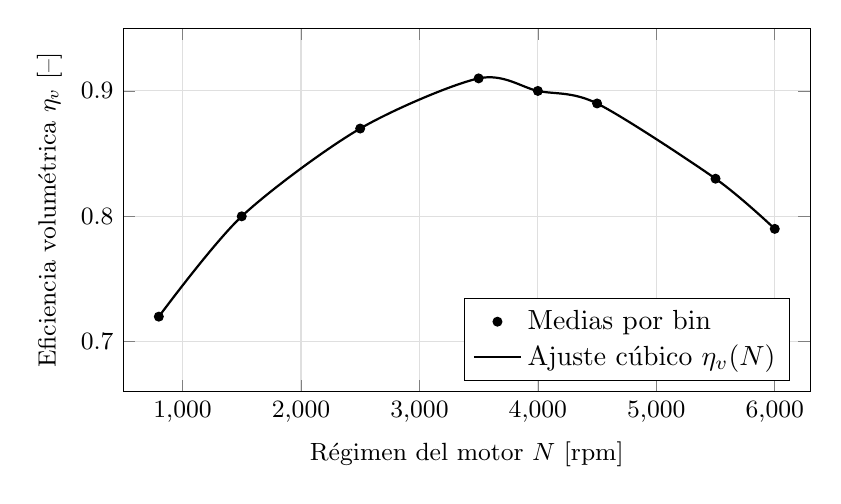
\begin{tikzpicture}
		\begin{axis}[
			width=0.85\textwidth, height=6.2cm,
			xlabel={Régimen del motor $N$ [rpm]},
			ylabel={Eficiencia volumétrica $\eta_v$ [--]},
			xmin=500, xmax=6300, ymin=0.66, ymax=0.95,
			grid=both, grid style={gray!25},
			legend pos=south east, legend cell align=left,
			tick label style={font=\small}, label style={font=\small},
			]
			\addplot[only marks, mark=*, mark size=1.6pt]
			coordinates {(800,0.72)(1500,0.80)(2500,0.87)(3500,0.91)
				(4000,0.90)(4500,0.89)(5500,0.83)(6000,0.79)};
			\addlegendentry{Medias por bin}
			\addplot[thick, smooth]
			coordinates {(800,0.72)(1500,0.80)(2500,0.87)(3500,0.91)
				(4000,0.90)(4500,0.89)(5500,0.83)(6000,0.79)};
			\addlegendentry{Ajuste cúbico $\eta_v(N)$}
		\end{axis}
	\end{tikzpicture}
	
	\vspace{2pt}
	{\footnotesize\textit{Nota.} Elaboración propia. Datos ilustrativos; los valores definitivos se obtienen del trayecto de calibración del vehículo de ensayo.}

\end{figure}

% --- Figura sugerida adicional (a generar con datos medidos): --------------------
% Se recomienda incluir una figura de validación con datos reales del vehículo,
% contrastando: (i) el estimado por muestra h\^{eta}_v (dispersión) frente al ajuste
% cúbico; y (ii) el consumo acumulado en lazo abierto vs. lazo cerrado vs. medición
% tanque-a-tanque. Plantilla:
%
% \begin{figure}[htbp]
	%   \centering
	%   \includegraphics[width=0.85\textwidth]{figuras/validacion_lazo.png}
	%   \caption{Comparación del consumo acumulado: estimación en lazo abierto,
		%   estimación en lazo cerrado y referencia tanque-a-tanque sobre la ruta de prueba.}
	%   \label{fig:validacion-lazo}
	%   % Nota (APA): Elaboración propia a partir de los datos de campo del vehículo de ensayo.
	% \end{figure}

% ------------------------------------------------------------------------------
\subsection{Modelo matemático final y variables de entrada/salida}
\label{subsec:modelo-final}

Reuniendo las ecuaciones anteriores, el modelo completo del estimador en lazo cerrado
se expresa como la siguiente cadena de cálculo. A partir de las entradas OBD-II y de
los parámetros del vehículo, el sistema produce el caudal instantáneo de combustible
y las métricas derivadas:

\begin{align}
	\rho &= \frac{P_{\text{MAP}}}{R\,T_{\text{IAT}}}, \label{eq:fin-rho}\\[2pt]
	\dot m_{\text{air}} &= \eta_v(N)\,\frac{P_{\text{MAP}}\,V_d\,N}{120\,R\,T_{\text{IAT}}}, \label{eq:fin-maire}\\[2pt]
	\dot m_{\text{fuel,SD}} &= \frac{\dot m_{\text{air}}}{\mathrm{AFR}_s\,\lambda}, \label{eq:fin-msd}\\[2pt]
	\dot m_{\text{fuel}} &= K\,\dot m_{\text{fuel,SD}}\left(1+\frac{\mathrm{STFT}}{100}\right), \label{eq:fin-mcorr}\\[2pt]
	\dot V_{\text{fuel}} &= \frac{\dot m_{\text{fuel}}}{\rho_{\text{fuel}}}, \label{eq:fin-vol}
\end{align}

con $\mathrm{AFR}_s = 14{,}7$, $R = 287\ \mathrm{J/(kg\cdot K)}$ y
$\rho_{\text{fuel}} \approx 745\ \mathrm{kg/m^3}$. Las métricas de salida se obtienen
por conversión de unidades e integración temporal:

\begin{align}
	Q_{\text{inst}}\,[\mathrm{L/h}] &= \dot V_{\text{fuel}}\times 3{,}6\times 10^{6}, \label{eq:fin-Lh}\\[2pt]
	Q_{\text{dist}}\,[\mathrm{L/100\,km}] &= \frac{Q_{\text{inst}}}{v}\times 100, \label{eq:fin-L100}\\[2pt]
	V_{\text{total}}\,[\mathrm{L}] &= \int_0^{t} \dot V_{\text{fuel}}\,\mathrm{d}t, \label{eq:fin-Vtot}\\[2pt]
	\text{Costo}\,[\mathrm{Bs}] &= V_{\text{total}}\times \text{precio}\,[\mathrm{Bs/L}], \label{eq:fin-costo}
\end{align}

donde $v$ es la velocidad del vehículo (PID~\texttt{0x0D}). El factor $3{,}6\times
10^{6}$ convierte $\mathrm{m^3/s}$ a $\mathrm{L/h}$
($\times 10^{3}\,\mathrm{L/m^3}\times 3600\,\mathrm{s/h}$). La
Tabla~\ref{tab:io-modelo} consolida todas las variables de entrada, los parámetros y
las salidas del modelo.

\begin{table}[htbp]
	
	\captionsetup{labelformat=simple, labelsep=newline, textfont=it, labelfont=bf, justification=raggedright, singlelinecheck=false}
	\caption{Variables de entrada, parámetros y salidas del modelo en lazo cerrado.}
	\centering
	\label{tab:io-modelo}
	\begin{tabular}{@{}llll@{}}
		\toprule
		\rowcolor[rgb]{0.851, 0.851, 0.851}
		\textbf{Categoría} & \textbf{Variable} & \textbf{Origen / valor} & \textbf{Unidad} \\
		\midrule
		\multirow{7}{*}{Entradas (OBD-II)}
		& $N$              & PID \texttt{0x0C} & rpm \\
		& $P_{\text{MAP}}$ & PID \texttt{0x0B} & kPa \\
		& $T_{\text{IAT}}$ & PID \texttt{0x0F} & $^{\circ}$C $\to$ K \\
		& $\lambda$        & PID \texttt{0x44} & -- \\
		& $\mathrm{STFT}$  & PID \texttt{0x06} & \% \\
		& $\mathrm{LTFT}$  & PID \texttt{0x07} & \% \\
		& $v$              & PID \texttt{0x0D} & km/h \\
		\midrule
		\multirow{6}{*}{Parámetros}
		& $V_d$            & Ficha del vehículo & m$^3$ \\
		& $\mathrm{AFR}_s$ & 14,7 (gasolina)    & -- \\
		& $\rho_{\text{fuel}}$ & $\approx 745$  & kg/m$^3$ \\
		& $R$              & 287                & J/(kg$\cdot$K) \\
		& $\eta_v(N)$      & Identificada (Alg.~\ref{alg:etav}) & -- \\
		& $\alpha_K,\,\alpha_{\eta_v}$ & 0,20 / 0,05 & -- \\
		\midrule
		\multirow{2}{*}{Estados adaptativos}
		& $K$              & EMA, $\in[0{,}70,\,1{,}30]$ & -- \\
		& $\eta_v[k]$      & Bins por régimen   & -- \\
		\midrule
		\multirow{6}{*}{Salidas}
		& $\dot m_{\text{air}}$  & Ec.~\eqref{eq:fin-maire} & kg/s \\
		& $\dot m_{\text{fuel}}$ & Ec.~\eqref{eq:fin-mcorr} & kg/s \\
		& $Q_{\text{inst}}$      & Ec.~\eqref{eq:fin-Lh}    & L/h \\
		& $Q_{\text{dist}}$      & Ec.~\eqref{eq:fin-L100}  & L/100\,km \\
		& $V_{\text{total}}$     & Ec.~\eqref{eq:fin-Vtot}  & L \\
		& Costo                  & Ec.~\eqref{eq:fin-costo} & Bs \\
		\bottomrule
	\end{tabular}
	
	\vspace{2pt}
	{\footnotesize\textit{Nota.} Elaboración propia.}
\end{table}

En síntesis, el modelo final propuesto integra la predicción física del método
Speed-Density (Ecuaciones~\eqref{eq:fin-rho}--\eqref{eq:fin-msd}) con dos
mecanismos de realimentación de distinta escala temporal: la corrección rápida
del $\mathrm{STFT}$ y la adaptación lenta del factor $K$
(Ecuación~\eqref{eq:fin-mcorr}), apoyados en una curva de eficiencia
volumétrica $\eta_v(N)$ identificada de los propios datos del vehículo. Esta
arquitectura de estimador en lazo cerrado está diseñada para convertir una
estimación abierta sensible al error de $\eta_v$ en un sistema robusto,
autocalibrable y trazable frente a una referencia física. Como se precisó al
inicio de la sección, el prototipo evaluado en el Capítulo~4 implementa el
subconjunto de esta arquitectura correspondiente a la corrección directa por
$\mathrm{STFT}+\mathrm{LTFT}$; el factor $K$ adaptativo y la identificación en
línea de $\eta_v(N)$ quedan formalizados como la vía de mejora que el
Capítulo~6 recomienda para satisfacer, en una versión futura del firmware, los
requisitos de exactitud y confiabilidad de largo plazo del proyecto.



% =====================================================================
%  SECCIÓN: Diseño de software
%  Tesis: Sistema de monitoreo de consumo OBD-II (ESP32 + SN65HVD230)
%  Autor: Erick — Ing. Mecatrónica, UMSA (La Paz, Bolivia)
% ---------------------------------------------------------------------
%  Requiere (ya presentes en tu preámbulo corregido):
%    listings, booktabs, multirow, tikz (shapes.geometric, arrows.meta,
%    positioning, calc), amsmath, natbib, graphicx, float, \pct
% =====================================================================

\section{Diseño de software}
\label{sec:software}

El código completo del firmware descrito en esta sección está disponible en el repositorio de GitHub del proyecto \citep{CalleGitHub2026}, carpeta \texttt{CODIGOS/esp32s3\_obd2\_speeddensity/}.

Esta sección retoma el capítulo de diseño de software y describe, parte por
parte, el firmware que corre en el ESP32-S3: las herramientas con las que se
construyó, cómo reparte el trabajo entre tareas, el protocolo con el que
habla con el vehículo, el método de cálculo del consumo, cómo persiste los
datos, cómo expone un panel de control, y el criterio detrás de cada
elección de componente y de librería.

% ============================================================
\subsection{Herramientas y entorno de desarrollo}
\label{sec:herramientas}
% ============================================================

\subsubsection{Visual Studio Code + PlatformIO}
El firmware se desarrolla en Visual Studio Code con la extensión PlatformIO
IDE, en vez del IDE oficial de Arduino. La diferencia no es cosmética:

\begin{itemize}
	\item \textbf{Toolchain embebido integrado.} PlatformIO gestiona la
	descarga y versión exacta del framework
	(\texttt{framework-arduinoespressif32}) \citep{arduinoesp32core2024},
	el compilador cruzado (\texttt{toolchain-xtensa-esp32s3}) y
	\texttt{esptool} para programar, todo declarado y fijado en
	\texttt{platformio.ini} \citep{platformio2024}. Esto hace que el
	\textit{build} sea reproducible entre máquinas (un requisito real
	una vez que el proyecto tiene múltiples archivos fuente y
	dependencias externas), algo que el modelo de ``sketch único'' del
	IDE de Arduino maneja peor.
	\item \textbf{Autocompletado real de C++.} Con un servidor de lenguaje
	indexando todo el árbol de \texttt{src/}/\texttt{include/}, moverse
	entre los siete archivos fuente del proyecto y sus cabeceras
	compartidas (\texttt{config.h}, \texttt{types.h}) es inmediato.
	\item \textbf{Terminal integrado.} Compilar, subir y abrir el monitor
	serie desde el mismo terminal donde se edita el código evita el
	cambio de contexto entre editor y herramienta externa, y deja el
	registro de errores de compilación con enlaces directos a archivo y
	línea.
\end{itemize}

\subsubsection{Por qué FreeRTOS}
Un sistema que a la vez sondea un bus CAN sensible a tiempos, refresca una
pantalla, escribe en una tarjeta SD y sirve un panel web por WiFi es, por
naturaleza, un problema \textbf{concurrente}. Hay dos formas razonables de
resolverlo: un único \texttt{loop()} con máquinas de estado manuales y
sondeo no bloqueante en cada punto donde se podría esperar (viable en
proyectos pequeños, pero frágil a medida que crecen), o un sistema operativo
de tiempo real con prioridades y primitivas de sincronización reales. Este
proyecto usa la segunda opción.

FreeRTOS no es, en rigor, una dependencia externa que se agregó, es el
planificador que el propio núcleo Arduino-ESP32 ya usa por debajo
\citep{freertos2024}; usarlo explícitamente es aprovechar la plataforma en
vez de pelear contra ella con un \texttt{loop()} monolítico encima.
Concretamente, esto permite:

\begin{itemize}
	\item Darle al sondeo CAN la \textbf{prioridad más alta} de todas las
	tareas, garantizando que una transacción I2C lenta hacia el OLED o
	una descarga de CSV por WiFi nunca retrase la lectura del vehículo.
	\item Proteger el estado compartido con mutex reales en vez de banderas
	improvisadas.
	\item Que agregar una funcionalidad nueva sea, casi siempre, agregar una
	tarea nueva con una prioridad clara, en vez de insertar más lógica
	condicional dentro de un bucle ya complejo: el modo de bajo consumo
	de la Sección~\ref{sec:idle} solo requirió tocar el bucle de la
	tarea CAN y agregar una bandera de estado que las demás tareas ya
	sabían consultar.
\end{itemize}

\begin{figure}[H]
	\centering
	\caption{\textit{Creación de tareas FreeRTOS en \texttt{src/main.cpp}.}}
	\label{fig:tasks}
	\begin{lstlisting}[language=C++, basicstyle=\fontsize{10}{10}\ttfamily, breaklines=true]
statusLedsInit();
xTaskCreatePinnedToCore(statusLedsTask, "leds", STACK_LED_TASK, nullptr,
PRIO_LED_TASK, nullptr, CORE_LED_TASK);
		
bool oledOk = displayInit();
bool sdOk   = sdLoggerInit();
bool canOk  = canObd2Init();
		
webServerInit(); // reporta ErrorCode::WIFI_FAIL si el softAP falla
		
if (canOk) {
	xTaskCreatePinnedToCore(canObd2Task, "canObd2", STACK_CAN_TASK, nullptr,
	PRIO_CAN_TASK, nullptr, CORE_CAN_TASK);
}
if (oledOk) {
	xTaskCreatePinnedToCore(displayTask, "display", STACK_DISPLAY_TASK, nullptr,
	PRIO_DISPLAY_TASK, nullptr, CORE_DISPLAY_TASK);
}
if (sdOk) {
	xTaskCreatePinnedToCore(sdLoggerTask, "sdLogger", STACK_SD_TASK, nullptr,
	PRIO_SD_TASK, nullptr, CORE_SD_TASK);
}
	\end{lstlisting}
	\begin{minipage}{\linewidth}
		\small
		\textit{Nota.} Inicialización condicional de las tareas asignadas a los núcleos del ESP32 según el estado de la verificación del hardware.
	\end{minipage}
\end{figure}

% ============================================================
\subsection{Interfaz con el hardware}
% ============================================================

El software está organizado alrededor de las interfaces físicas del
ESP32-S3 \citep{espressif2024datasheet,espressif2024trm}. Cada periférico se
eligió por una razón concreta, no por ser ``lo que venía en el kit'':

\begin{table}[H]
	\centering
	\captionsetup{labelformat=simple, labelsep=newline, textfont=it, labelfont=bf, justification=raggedright, singlelinecheck=false}
	\caption{Mapa de pines definido en \texttt{include/config.h}.}
	\label{tab:mapa_pines}
	\begin{tabular}{lll}
		\toprule
		\rowcolor[rgb]{0.851, 0.851, 0.851}
		Bus & Señal & GPIO ESP32-S3 \\
		\midrule
		TWAI (CAN) & TX $\rightarrow$ SN65HVD230 CTX & GPIO4 \\
		TWAI (CAN) & RX $\leftarrow$ SN65HVD230 CRX  & GPIO5 \\
		I2C        & SDA $\rightarrow$ OLED          & GPIO8 \\
		I2C        & SCL $\rightarrow$ OLED          & GPIO9 \\
		SPI (SD)   & SCK                             & GPIO12 \\
		SPI (SD)   & MISO                            & GPIO13 \\
		SPI (SD)   & MOSI                            & GPIO11 \\
		SPI (SD)   & CS                              & GPIO10 \\
		LED        & CAN activo                      & GPIO15 \\
		LED        & Actividad SD                    & GPIO16 \\
		LED        & Servidor activo                 & GPIO18 \\
		LED        & Error                           & GPIO17 \\
		\bottomrule
	\end{tabular}
	\\
	\vspace{2mm}
	\begin{minipage}{\linewidth}
		\small
		\textit{Nota.} Asignación de pines del microcontrolador ESP32-S3 para los buses de comunicación CAN, I2C, SPI y los indicadores LED de estado.
	\end{minipage}
\end{table}

\textit{Nota.} Pines reservados (no usar): GPIO 26-37 (bus interno hacia el
flash y la PSRAM octal del módulo N16R8) y GPIO 0/3/19/20/43-46 (pines de
\textit{strapping}, USB nativo y consola UART0 del chip).

\subsubsection{Controlador CAN: TWAI integrado, no un chip externo}
El ESP32-S3 trae un controlador CAN (TWAI) integrado en el propio chip
\citep{espressif2024trm}. Esa es la razón por la que el diseño no usa un
controlador CAN externo por SPI como el MCP2515, común en proyectos sobre
Arduino Uno/Nano que no tienen esta capacidad de fábrica: usar el
controlador nativo ahorra un dispositivo, una interrupción y un bus SPI que
ya está ocupado por la microSD, y evita la latencia adicional de tener que
serializar cada trama CAN a través de otro periférico intermediario.

\subsubsection{Transceptor CAN: SN65HVD230}
El TWAI del ESP32-S3 solo genera niveles lógicos TTL; convertirlos a las
señales diferenciales CAN\_H/CAN\_L del bus físico requiere un transceptor.
Se eligió el SN65HVD230 \citep{sn65hvd230_datasheet} en concreto porque opera
nativamente a 3.3\,V, el mismo nivel lógico del ESP32-S3; así se evita un
\textit{level-shifter} que sí haría falta con transceptores clásicos de 5\,V
como el MCP2551. CAN\_H y CAN\_L se conectan a los pines 6 y 14 del conector
OBD2 (J1962).

\subsubsection{Pantalla: SSD1306 OLED por I2C}
Se eligió un OLED monocromático de $128\times64$ px con controlador SSD1306
\citep{solomon2008ssd1306} sobre I2C en vez de, por ejemplo, una pantalla TFT
a color por SPI, por tres razones: consume solo 2 pines (I2C) dejando el SPI
libre para la SD; su consumo (10-20\,mA encendida, y se puede apagar por
software, Sección~\ref{sec:idle}) es bajo comparado con un TFT retroiluminado;
y la resolución alcanza de sobra para los pocos números grandes que hace
falta mostrar al conductor (no se necesita color ni gráficos complejos en el
tablero físico: eso ya lo cubre el panel web).

\subsubsection{Almacenamiento: microSD por SPI dedicado}
La tarjeta microSD usa su propio bus SPI, sin compartirlo con ningún otro
periférico. La alternativa, reutilizar un bus SPI ya en uso, se descartó
porque el registro en la SD ocurre una vez por segundo de forma predecible
mientras que una eventual escritura de mayor tamaño (por ejemplo, servir una
descarga de CSV completa) no debe competir por el bus con otra
responsabilidad no relacionada; un bus dedicado simplifica el análisis de
tiempos y evita tener que coordinar dos periféricos distintos sobre el mismo
SPI.

% ============================================================
\subsection{Arquitectura de tareas}
% ============================================================

\begin{table}[H]
	\centering
	\captionsetup{labelformat=simple, labelsep=newline, textfont=it, labelfont=bf, justification=raggedright, singlelinecheck=false}
	\caption{Tareas FreeRTOS, definidas en \texttt{include/config.h} y creadas en \texttt{src/main.cpp}.}
	\label{tab:tareas_freertos}
	\begin{tabular}{llccc}
		\toprule
		\rowcolor[rgb]{0.851, 0.851, 0.851}
		Tarea & Función & Núcleo & Prioridad & Pila (bytes) \\
		\midrule
		CAN/OBD2       & \texttt{canObd2Task}       & 0 & 5 & 4096 \\
		SD logger      & \texttt{sdLoggerTask}      & 1 & 4 & 6144 \\
		WebSocket push & \texttt{webSocketPushTask} & 0 & 3 & 4096 \\
		OLED display   & \texttt{displayTask}       & 1 & 2 & 4096 \\
		LEDs de estado & \texttt{statusLedsTask}    & 1 & 1 & 2048 \\
		\bottomrule
	\end{tabular}
	\\
	\vspace{2mm}
	\begin{minipage}{\linewidth}
		\small
		\textit{Nota.} Distribución de tareas en el sistema operativo en tiempo real FreeRTOS, especificando la asignación de núcleos del ESP32, prioridades de ejecución y tamaño de pila asignado a cada hilo.
	\end{minipage}
\end{table}

El núcleo 0 concentra lo sensible a tiempos (sondeo CAN de alta prioridad +
la pila WiFi/AsyncTCP, que en Arduino-ESP32 corre en ese mismo núcleo). El
núcleo 1 queda con las tareas de interfaz/almacenamiento, que toleran más
\textit{jitter} sin afectar la lectura del vehículo. Las prioridades no son
arbitrarias: reflejan directamente qué tan caro es que cada tarea llegue
tarde (perder un ciclo de sondeo CAN corrompe el cálculo de consumo; llegar
tarde a refrescar un LED es imperceptible).

\subsubsection{Sincronización entre tareas}
Dos mutex protegen el estado compartido: \texttt{g\_dataMutex} protege
\texttt{g\_vehicleData} (la tarea CAN arma cada ciclo en una copia local y
solo toca la estructura global, bajo mutex, en el paso final de fusión,
ver Figura~\ref{fig:merge}); \texttt{g\_sdMutex} protege el bus SPI de la
microSD, compartido entre el \textit{logger} periódico y los endpoints de
descarga/gráfica del servidor web. El criterio para usar mutex en vez de,
por ejemplo, deshabilitar interrupciones o copiar datos sin protección, es
que ambos recursos (la estructura de datos y el bus SPI) tienen escritores y
lectores en tareas de distinta prioridad corriendo en núcleos distintos: un
mutex es la primitiva correcta quando el acceso puede, en principio,
bloquear brevemente sin romper los tiempos críticos del sistema.



\begin{figure}[H]
	\centering
	\caption{\textit{Fusión bajo mutex al final de cada ciclo, \texttt{src/can\_obd2.cpp}.}}
	\label{fig:merge}
	\begin{lstlisting}[language=C++, basicstyle=\fontsize{10}{10}\ttfamily, breaklines=true]
if (xSemaphoreTake(g_dataMutex, pdMS_TO_TICKS(100)) == pdTRUE) {
	VehicleData &g = g_vehicleData;
	g.rpm = scratch.rpm;
	g.speed_kmh = scratch.speed_kmh;
	// ... resto de los campos ...
	g.can_status = status;
	g.data_valid = criticalOk;
	g.last_update_ms = now;
			
	if (criticalOk && dt > 0.0f && dt < 5.0f) {
		fuelCalcUpdate(g, dt);
	}
	xSemaphoreGive(g_dataMutex);
}
	\end{lstlisting}
	\begin{minipage}{\linewidth}
		\small
		\textit{Nota.} Sincronización de variables del vehículo mediante semáforo mutex para garantizar la integridad de los datos compartidos entre tareas en FreeRTOS.
	\end{minipage}
\end{figure}

\subsubsection{Manejo de errores}
\texttt{systemReportError(ErrorCode)} centraliza el reporte de fallos: guarda
el último código en \texttt{g\_systemStatus.error\_code} (dispara el parpadeo
del LED de error) y lo imprime por \texttt{Serial} con el detalle completo.
El criterio es separar dos audiencias distintas: el LED es para el
conductor, que solo necesita saber \textit{que algo falló}; el log serie es
para depuración en banco, donde sí importa el detalle completo y el
historial.

\begin{table}[H]
	\centering
	\captionsetup{labelformat=simple, labelsep=newline, textfont=it, labelfont=bf, justification=raggedright, singlelinecheck=false}
	\caption{Códigos de \texttt{ErrorCode} (\texttt{include/types.h}).}
	\label{tab:error_codes}
	\begin{tabular}{cl}
		\toprule
		\rowcolor[rgb]{0.851, 0.851, 0.851}
		Código & Significado \\
		\midrule
		1 & Fallo al iniciar el driver TWAI/CAN \\
		2 & Fallo al iniciar la microSD \\
		3 & Fallo al iniciar la pantalla OLED \\
		4 & Fallo al iniciar el punto de acceso Wi-Fi \\
		\bottomrule
	\end{tabular}
	\\
	\vspace{2mm}
	\begin{minipage}{\linewidth}
		\small
		\textit{Nota.} Identificación numérica de errores de inicialización del hardware y periféricos empleada por el sistema para el diagnóstico.
	\end{minipage}
\end{table}

% ============================================================
\subsection{Protocolo CAN / OBD2}
% ============================================================

El controlador TWAI del ESP32-S3 se configura a \textbf{500\,kbit/s}, el
estándar de la mayoría de vehículos livianos con OBD2 sobre CAN
(ISO 15765-4, \citep{iso157654}). Todas las
peticiones usadas caben en un único \textit{frame} CAN de 8 bytes
(\textit{single frame}), así que no hace falta implementar el mecanismo
multi-\textit{frame} de control de flujo ISO-TP (una simplificación
deliberada: ninguno de los PIDs que este proyecto necesita supera ese
tamaño, y soportar multi-\textit{frame} sin necesitarlo solo agrega
superficie de error).

\subsubsection{PIDs consultados (Modo 01)}
El conjunto de PIDs se eligió por ser el mínimo necesario para el cálculo
speed-density (Sección~\ref{sec:speeddensity}) más los que enriquecen el
registro sin costo relevante de tiempo de bus, siguiendo el estándar SAE
J1979 \citep{sae_j1979_2014}:

\begin{table}[H]
	\centering
	\captionsetup{labelformat=simple, labelsep=newline, textfont=it, labelfont=bf, justification=raggedright, singlelinecheck=false}
	\caption{PIDs Mode 01 consultados por \texttt{canObd2Task}.}
	\label{tab:pids_mode01}
	\begin{tabular}{cll}
		\toprule
		\rowcolor[rgb]{0.851, 0.851, 0.851}
		PID & Dato & Uso \\
		\midrule
		\texttt{0x0C} & RPM & Speed-density (crítico) \\
		\texttt{0x0B} & MAP (kPa) & Speed-density (crítico) \\
		\texttt{0x0F} & IAT (°C) & Speed-density (crítico) \\
		\texttt{0x0D} & Velocidad (km/h) & L/100km, distancia (crítico) \\
		\texttt{0x05} & Temperatura refrigerante & Mostrado en pantalla/CSV \\
		\texttt{0x04} & Carga calculada (\%) & Mostrado en pantalla/CSV \\
		\texttt{0x06} & Fuel trim corto plazo (\%) & Corrige el AFR estimado \\
		\texttt{0x07} & Fuel trim largo plazo (\%) & Corrige el AFR estimado \\
		\bottomrule
	\end{tabular}
	\\
	\vspace{2mm}
	\begin{minipage}{\linewidth}
		\small
		\textit{Nota.} Identificadores de parámetros (PIDs) solicitados mediante el protocolo OBD-II para el cálculo del consumo instantáneo de combustible y monitoreo de sensores.
	\end{minipage}
\end{table}
\textit{Nota.} Los cuatro PIDs marcados ``crítico'' son indispensables para el
cálculo speed-density; si la ECU no responde alguno, el ciclo completo se
marca inválido y no se integra al viaje.

\subsubsection{Formato de la petición}

\begin{figure}[H]
	\centering
	\caption{\textit{Trama de petición Mode 01, PID genérico.}}
	\label{fig:trama_obd2}
	\begin{lstlisting}[language=C++, basicstyle=\fontsize{10}{10}\ttfamily, breaklines=true]
ID = 0x7DF
Data[0] = 0x02   ; SF, 2 bytes de payload (modo + pid)
Data[1] = 0x01   ; Modo 01: datos actuales
Data[2] = <PID>
Data[3..7] = 0x00 (relleno)
	\end{lstlisting}
	\begin{minipage}{\linewidth}
		\small
		\textit{Nota.} Estructura de la trama CAN empleada para la solicitud de parámetros OBD-II en el vehículo.
	\end{minipage}
\end{figure}

Las ECUs responden en el rango \texttt{0x7E8}-\texttt{0x7EF}; se acepta la
primera respuesta cuyo \texttt{Data[1] == 0x41} y \texttt{Data[2]} coincida
con el PID pedido.

\subsubsection{Recuperación de bus-off}
Si el controlador entra en estado \texttt{BUS\_OFF}, la recuperación se
sondea en cada vuelta del bucle sin bloquear con una espera fija: según el
driver TWAI de ESP-IDF \citep{espressif2024trm}, la recuperación solo llega a
\texttt{STOPPED} tras contar 128 ocurrencias de 11 bits recesivos
consecutivos en el bus, un tiempo que depende del tráfico real y no se puede
predecir de antemano; sondear en vez de esperar un tiempo fijo evita tanto
reintentar demasiado pronto (fallar en vano) como esperar de más
innecesariamente.

% ============================================================
\subsection{Método de cálculo: Speed-Density}
\label{sec:speeddensity}
% ============================================================

El método speed-density estima el flujo másico de aire admitido por el motor
a partir de la ley de gases ideales, sin medirlo con un sensor MAF (la
razón de fondo para elegir este método sobre uno basado en MAF real es que
la mayoría de los vehículos con OBD2 reportan MAP, no flujo de aire directo,
así que speed-density es el único método viable sin instalar un sensor
adicional):

\begin{equation}
	\dot{m}_{aire} \;[\text{g/s}] =
	\frac{\dfrac{VE}{100} \cdot RPM \cdot MAP\,[\text{kPa}] \cdot V_d\,[\text{L}] \cdot 28.97}
	{2 \cdot 8.314 \cdot T_{IAT}\,[\text{K}] \cdot 60}
\end{equation}

donde $VE$ es la eficiencia volumétrica (\%) interpolada de una tabla
calibrable (Sección~\ref{sec:ve}); $V_d$ la cilindrada en litros; $28.97$ la
masa molar del aire (g/mol); $8.314$ la constante universal de los gases
(L$\cdot$kPa/(mol$\cdot$K)); el factor $2$ corresponde a que un motor de 4
tiempos completa una admisión cada 2 vueltas de cigüeñal; y $T_{IAT}$ la
temperatura de admisión en Kelvin, con guarda de rango
[$-40$,\,$100$]\,\textdegree C.

\begin{figure}[H]
	\centering
	\caption{\textit{Núcleo del cálculo speed-density, \texttt{src/fuel\_calc.cpp}.}}
	\label{fig:fuelcalc}
	\begin{lstlisting}[language=C++, basicstyle=\fontsize{10}{10}\ttfamily, breaklines=true]
float ve = fuelCalcVeForRpm(vd.rpm);
float iat_K = vd.iat_c + 273.15f;
if (iat_K < 233.15f || iat_K > 373.15f) iat_K = 288.15f;
		
const float MM_AIR = 28.97f; // g/mol
const float R = 8.314f;      // L*kPa/(mol*K)
		
float maf = (ve / 100.0f) * (float)vd.rpm * vd.map_kpa *
ENGINE_DISPLACEMENT_L * MM_AIR /(2.0f * R * iat_K * 60.0f);
	\end{lstlisting}
	\begin{minipage}{\linewidth}
		\small
		\textit{Nota.} Algoritmo para la estimación del flujo de masa de aire (MAF) a partir de la eficiencia volumétrica (VE), presión MAP y temperatura IAT.
	\end{minipage}
\end{figure}

\subsubsection{De aire a combustible}

\begin{equation}
	\dot{m}_{comb}\,[\text{g/s}] = \frac{\dot{m}_{aire}}{AFR} \cdot k_{cal}
\end{equation}

$AFR$ es la relación aire/combustible, por defecto el valor estequiométrico
de la gasolina ($AFR_{stoich} = 14.7$), opcionalmente corregido con los
\textit{fuel trims} que reporta la ECU:

\begin{equation}
	AFR_{efectivo} = \frac{AFR_{stoich}}{1 + \frac{STFT\% + LTFT\%}{100}}
\end{equation}

acotado a $[8, 25]$. $k_{cal}$ es \texttt{FUEL\_CALIBRATION\_FACTOR}
(Sección~\ref{sec:calibracion}), $1.0$ por defecto. El criterio para incluir
la corrección por \textit{fuel trim} es que, sin ella, el cálculo asume que
el motor siempre corre exactamente en estequiométrico, cosa que en la
práctica no ocurre; usar los \textit{trims} que la propia ECU ya reporta es
una corrección ``gratis'' (no requiere sensores adicionales) frente a un error
sistemático conocido.

\subsubsection{De masa a volumen}

\begin{align}
	\dot{V}_{comb}\,[\text{L/h}] &= \frac{\dot{m}_{comb} \cdot 3600}{\rho_{comb}} \\[4pt]
	L/100km &=
	\begin{cases}
		\dfrac{\dot{V}_{comb}}{v}\cdot 100 & \text{si } v > 2\,\text{km/h} \\[6pt]
		0 & \text{vehículo detenido}
	\end{cases}
\end{align}

con $\rho_{comb} = 745\,\text{g/L}$ y $v$ la velocidad en km/h.

\subsubsection{Integración del viaje}

\begin{align}
	L_{viaje} &\mathrel{+}= \dot{m}_{comb} \cdot dt \,/\, \rho_{comb} \\
	km_{viaje} &\mathrel{+}= v \cdot dt / 3600 \\
	Bs_{viaje} &= L_{viaje} \cdot P_{L}
\end{align}

con $dt$ el paso de tiempo real entre ciclos (no un valor fijo, precisamente
para no perder precisión si un ciclo de sondeo tarda más o menos de lo
típico) y $P_L = 6.96$ (\texttt{FUEL\_PRICE\_BS\_PER\_L}) el precio de
referencia del litro.

\subsubsection{Tabla de eficiencia volumétrica (VE)}
\label{sec:ve}

\begin{table}[H]
	\centering
	\captionsetup{labelformat=simple, labelsep=newline, textfont=it, labelfont=bf, justification=raggedright, singlelinecheck=false}
	\caption{\texttt{kVeTable}, \texttt{src/fuel\_calc.cpp}. Interpolación lineal entre puntos.}
	\label{tab:ve_table}
	\begin{tabular}{ccl}
		\toprule
		\rowcolor[rgb]{0.851, 0.851, 0.851}
		RPM & VE (\%) & Origen \\
		\midrule
		940  & 82.7 & Calibrado (Nissan Vanette) \\
		1500 & 79.7 & Calibrado (Nissan Vanette) \\
		2500 & 79.7 & Calibrado (Nissan Vanette) \\
		3500 & 72.7 & Calibrado (Nissan Vanette) \\
		4000 & 88.0 & Genérico, sin calibrar \\
		5500 & 83.0 & Genérico, sin calibrar \\
		7000 & 74.0 & Genérico, sin calibrar \\
		\bottomrule
	\end{tabular}
	\vspace{2mm}
	\begin{minipage}{\linewidth}
		\small
		\textit{Nota.} Tabla de valores de eficiencia volumétrica (VE) caracterizados según el régimen de rotación del motor (RPM) para la estimación del flujo de masa de aire mediante el método speed-density.
	\end{minipage}
\end{table}

\textit{Nota.} Los cuatro puntos marcados como ``Calibrado'' se obtuvieron
con la prueba estática de pasos de RPM del Nissan Vanette contra su PID
0x10/MAF real (Sección~4.3.3 del Capítulo~4); el procedimiento de
calibración general se documenta en la Subsección~\ref{sec:ve-general}. Los
puntos restantes (4000/5500/7000\,rpm) son un punto de partida genérico, no
un dato de fábrica del vehículo: sin calibrarlos, el consumo calculado en
ese rango tendrá un error sistemático.

\subsubsection{Cálculo general de la eficiencia volumétrica para un vehículo arbitrario}
\label{sec:ve-general}

Los cuatro puntos calibrados de la Tabla~\ref{tab:ve_table} son específicos
del Nissan Vanette: no existen dos motores con la misma curva $\eta_v$, así
que no es razonable pedirle a un código un número universal de eficiencia
volumétrica. Lo que sí es general (y se documenta en esta subsección) es el
\emph{procedimiento} para calcularla a partir de datos reales de
\textbf{cualquier} vehículo, implementado en
\texttt{CODIGOS/ve\_curve\_calibrator.py} y disponible en el repositorio de
GitHub del proyecto \citep{CalleGitHub2026}.

\paragraph{Teoría.} La eficiencia volumétrica se define como el cociente
entre la masa de aire realmente admitida y la masa teórica que ocuparía la
cilindrada a la densidad de admisión (Ecuación~\eqref{eq:eta_v}). No es un
dato de fábrica del vehículo \citep{Heywood2018}: depende de la geometría de
válvulas, el árbol de levas, la resonancia de los múltiples de admisión y
escape, y el estado mecánico del motor: parámetros de diseño que ningún PID
OBD-II expone y que no admiten una fórmula cerrada válida para cualquier
motor. Por esto, en la práctica de la puesta a punto de motores (por
ejemplo, en sistemas de gestión programable tipo \textit{speed-density}) la
curva $\eta_v(N)$ siempre se obtiene de forma empírica, nunca analítica.

\paragraph{Ingeniería.} Lo que sí generaliza es la propia ecuación de
speed-density (Ecuación~\eqref{eq:speed_density}): dado un conjunto real de
muestras $(RPM, P_{MAP}, T_{IAT})$ y una referencia real de flujo de aire
$MAF_{ref}$ (el PID 0x10, cuando el vehículo lo soporta), se despeja
algebraicamente la única incógnita:

\begin{equation}
	VE_{\text{requerida}} = \frac{MAF_{ref} \cdot 100 \cdot 2 \cdot 8.314 \cdot T_{IAT} \cdot 60}{RPM \cdot P_{MAP} \cdot V_d \cdot 28.97}
	\label{eq:ve_general}
\end{equation}

Esta es la misma inversión de la Ecuación~\eqref{eq:speed_density} usada
para calibrar la Tabla~\ref{tab:ve_table} (Sección~4.3.3 del Capítulo~4),
pero aquí generalizada: el código no asume ningún vehículo, régimen objetivo
ni número fijo de puntos: solo necesita la cilindrada $V_d$ y un registro
CSV con columnas \texttt{rpm}, \texttt{map\_kpa}, \texttt{iat\_c} y
\texttt{maf\_referencia\_gs}, en el mismo formato que produce
\texttt{speed\_density\_bench.py}.

\begin{figure}[H]
	\centering
	\caption{Inversión general de la ecuación speed-density, \texttt{ve\_curve\_calibrator.py}.}
	\label{fig:ve_general_code}
	\begin{lstlisting}[language=Python, basicstyle=\fontsize{9}{10}\ttfamily, breaklines=true]
def estimate_ve(rpm, map_kpa, iat_c, maf_ref_gs, displacement_l):
    iat_k = iat_c + 273.15
    if iat_k < 233.15 or iat_k > 373.15:
        iat_k = 288.15
    return maf_ref_gs * 100.0 * 2.0 * R * iat_k * 60.0 \
           / (rpm * map_kpa * displacement_l * MM_AIR)
	\end{lstlisting}
	\begin{minipage}{\linewidth}
		\small
		\textit{Nota.} \texttt{displacement\_l} ($V_d$) es el único parámetro que cambia entre vehículos; el resto de la función es idéntico a la Ecuación~\eqref{eq:ve_general} para cualquier motor.
	\end{minipage}
\end{figure}

\paragraph{Criterio del programa.} Una sola muestra invertida es ruidosa
(cuantización de los PID, transitorios de conducción), así que el script no
reporta la VE muestra por muestra sino que sigue el mismo criterio de
agrupamiento y ajuste que el Algoritmo~\ref{alg:etav} del lazo cerrado
(Sección~\ref{sec:lazo-cerrado}), con una diferencia deliberada en la fuente
del estimado puntual:

\begin{itemize}
	\item \textbf{Agrupamiento por bin de régimen.} Las muestras se agrupan en
	intervalos de RPM de ancho configurable (250\,rpm por defecto), igual que
	la Ecuación~\eqref{eq:etav-cubica}, en vez de exigir puntos de régimen
	fijos como \texttt{calibrate\_ve\_table.py}: esto permite calibrar con
	cualquier registro de conducción, no solo con la prueba estática de pasos
	de RPM.
	\item \textbf{Umbral mínimo de confianza.} Un bin con menos de
	\texttt{min\_samples} muestras (5 por defecto) se marca como de baja
	confianza y se excluye del ajuste en vez de participar con un promedio
	poco confiable; no se rellena ningún bin sin datos suficientes con un
	valor supuesto.
	\item \textbf{Regresión cúbica ponderada.} Sobre los bins de confianza se
	ajusta el mismo polinomio cúbico $\eta_v(N)=c_0+c_1N+c_2N^2+c_3N^3$ de la
	Ecuación~\eqref{eq:etav-cubica}, ponderado por el número de muestras de
	cada bin, junto con su coeficiente de determinación $R^2$ para poder
	juzgar la calidad del ajuste en vez de aceptarlo a ciegas.
\end{itemize}

La diferencia con el Algoritmo~\ref{alg:etav} original es la fuente del
estimado puntual: aquel, pensado para ejecutarse en línea dentro del propio
firmware, infiere $\hat\eta_v$ de forma indirecta a partir del STFT/LTFT
(por lo que requiere ya conocer una curva semilla $\eta_v^0(N)$ para
funcionar, Ecuación~\eqref{eq:etav-estimado}), mientras que
\texttt{ve\_curve\_calibrator.py} lo calcula de forma directa a partir de un
$MAF_{ref}$ real, sin depender de ninguna curva previa. Por esta misma
razón, este script offline es además una forma práctica de generar esa
curva semilla $\eta_v^0(N)$ que el Algoritmo~\ref{alg:etav} necesita como
punto de partida, en cualquier vehículo que soporte el PID 0x10.

La Figura~\ref{fig:ve_curve_vanette} muestra el resultado de correr el
script sobre el mismo registro del Nissan Vanette (Sección~4.3.3 del
Capítulo~4, $V_d=1{,}626$\,L): a diferencia de la calibración de cuatro
puntos fijos, aquí se aprovechan también las muestras tomadas durante las
transiciones entre regímenes, lo que produce ocho bins de confianza en vez
de cuatro y permite juzgar la calidad del ajuste cúbico con un
$R^2=0{,}968$.

\begin{figure}[H]
	\centering
	\caption{Curva de eficiencia volumétrica identificada por \texttt{ve\_curve\_calibrator.py} sobre datos reales del Nissan Vanette}
	\label{fig:ve_curve_vanette}
	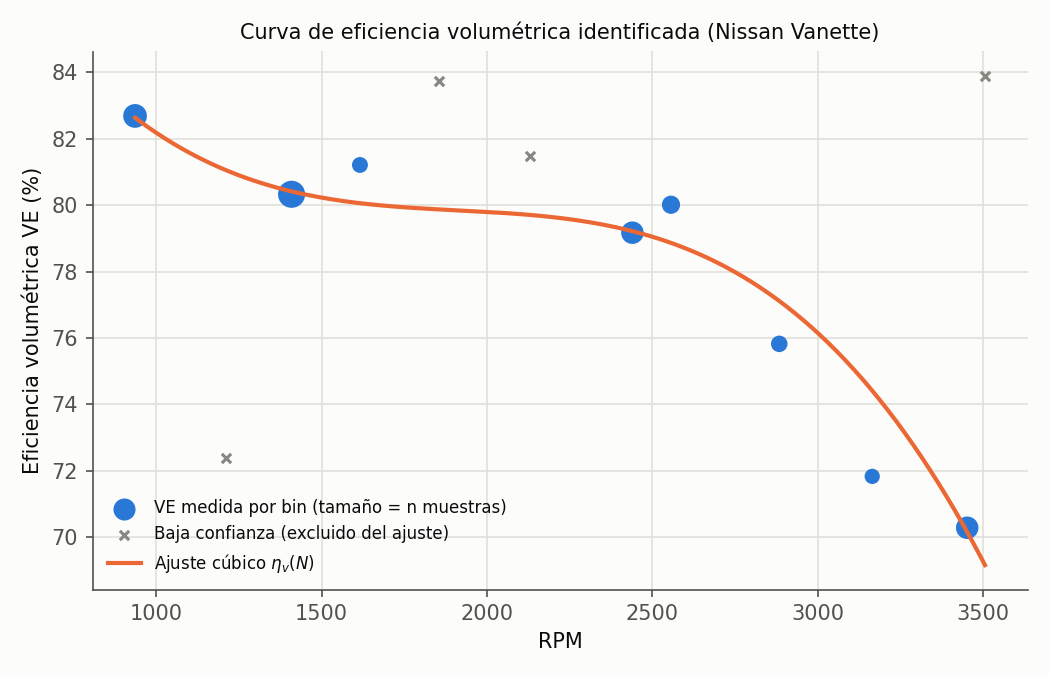
\includegraphics[width=0.8\textwidth]{Images/ve_curve_fit_vanette.png}

	\vspace{2pt}
	{\footnotesize\textit{Nota.} Círculos: VE promedio por bin (tamaño proporcional al número de muestras). Cruces: bins de baja confianza, excluidos del ajuste. Línea: polinomio cúbico ponderado, Ecuación~\eqref{eq:etav-cubica}. Elaboración propia.}
\end{figure}

\paragraph{Caso sin MAF: el Changan Honor.} La Ecuación~\eqref{eq:ve_general}
requiere una referencia real de flujo de aire ($MAF_{ref}$) para despejar la
VE de forma directa; sin ella, RPM, MAP e IAT por sí solos no alcanzan para
aislar esa incógnita. El Changan Honor no soporta el PID 0x10
(Tabla~\ref{tab:pids_verificacion}, Capítulo~4), así que
\texttt{ve\_curve\_calibrator.py} no es aplicable a este vehículo: ninguna
manipulación algebraica sustituye a la referencia real que falta.

El escaneo de PIDs del Changan (Apéndice~O) confirma, sin embargo, que sí
soporta el PID~0x06 (STFT), el PID~0x07 (LTFT) y el PID~0x44 (relación de
equivalencia aire-combustible comandada, usada aquí como indicador de lazo
cerrado). Esa combinación es exactamente la que requiere el
Algoritmo~\ref{alg:etav} ya formalizado en la Sección~\ref{sec:lazo-cerrado}:
en vez de una referencia absoluta de aire, usa el propio ajuste de mezcla
que la ECU ya reporta como señal indirecta de que la VE asumida está mal.
\texttt{CODIGOS/ve\_curve\_calibrator\_indirect.py} implementa una versión
offline de ese algoritmo, análoga en estructura a
\texttt{ve\_curve\_calibrator.py} (mismo agrupamiento por bin, mismo umbral
mínimo de confianza, mismo ajuste cúbico ponderado) pero con un estimador
puntual distinto, el de la Ecuación~\eqref{eq:etav-estimado}:

\begin{equation}
	\hat\eta_v(N) = \eta_v^{0}(N)\left(1 + \frac{\mathrm{STFT}\% + \mathrm{LTFT}\%}{100}\right)
\end{equation}

donde $\eta_v^{0}(N)$ es una curva semilla (por defecto, la misma tabla
genérica de literatura con la que este proyecto arrancó antes de calibrar la
del Vanette, Tabla~\ref{tab:ve_table}, valores originales) y solo se
aceptan muestras con el motor en lazo cerrado ($|\lambda_{cmd}-1|$ dentro de
una tolerancia, PID~0x44), descartando los tramos de enriquecimiento donde
el STFT/LTFT no reflejan un error de VE sino una estrategia distinta de la
ECU. Nótese que esta corrección es multiplicativa y relativa a la curva
semilla (no involucra $V_d$, $P_{MAP}$ ni $T_{IAT}$), a diferencia de la
Ecuación~\eqref{eq:ve_general}, que sí es una inversión absoluta de la
ecuación de gas ideal.

\textit{Advertencia epistemológica.} El resultado de este procedimiento
\textbf{no} debe reportarse como una VE ``calibrada'' del Changan en el mismo
sentido que la del Vanette: es una \emph{corrección relativa a una curva
semilla asumida}, no una medición absoluta. Si la curva semilla generica
está lejos de la realidad de este motor en particular, la corrección
heredará ese sesgo: el método solo garantiza mayor consistencia con los
STFT/LTFT observados, no exactitud absoluta, precisamente por la ausencia de
una referencia real de aire o combustible en este vehículo. Queda, junto con
la recolección misma de los datos con \texttt{CODIGOS/changan\_trim\_logger.py},
como trabajo pendiente para una eventual continuación de este proyecto
(Capítulo~6): no se generó una curva para el Changan dentro del alcance de
este trabajo por no haberse completado esa recolección de campo.

\subsubsection{Calibración contra un tanque real}
\label{sec:calibracion}
No existe forma de que el ESP32 sepa, por sí solo, si el número que calcula
es correcto (no hay con qué comparar dentro del propio microcontrolador).
El procedimiento recomendado: llenar el tanque y anotar el odómetro, manejar
con normalidad hasta la próxima recarga, comparar los litros reales cargados
contra \texttt{trip\_fuel\_L} acumulado en esa misma distancia, y ajustar

\begin{equation}
	\texttt{FUEL\_CALIBRATION\_FACTOR} = \frac{L_{real}}{L_{calculado}}
\end{equation}

en \texttt{config.h}. El criterio de aplicar un único factor multiplicativo
sobre \texttt{fuel\_gs}, en vez de reajustar toda la tabla VE a mano, es que
corrige de forma consistente el instantáneo, el acumulado del viaje y el
costo con un solo número, y es reversible/auditable, a diferencia de
retocar seis puntos de la tabla VE por prueba y error.

% ============================================================
\subsection{Registro en microSD}
% ============================================================

Cada arranque crea un archivo nuevo \texttt{/logs/trip\_NNN.csv} (índice
autoincremental calculado escaneando los archivos existentes, en vez de un
contador separado que podría desincronizarse tras un corte de energía). Se
escribe una fila por segundo, solo después del primer ciclo CAN válido, y se
pausa por completo durante el modo de bajo consumo (Sección~\ref{sec:idle}).

\subsubsection{Por qué CSV}
Se eligió CSV en vez de un formato binario compacto o JSON por fila por tres
razones: es directamente legible/abrible en cualquier hoja de cálculo sin
escribir un parser; el tamaño de fila (unos 100 bytes) es intrascendente
frente a la capacidad de una microSD moderna incluso a una fila por segundo
durante horas; y es el formato que el propio panel web ya necesita poder
descargar y volver a interpretar (Sección~\ref{sec:panelweb}), así que un
mismo formato sirve para ambos usos sin conversión intermedia.



\begin{figure}[H]
	\centering
	\caption{\textit{Fila de ejemplo del CSV (encabezado y fila de datos).}}
	\label{fig:csv_ejemplo}
	\begin{lstlisting}[language=C++, basicstyle=\fontsize{10}{10}\ttfamily, breaklines=true]
uptime_ms,rpm,speed_kmh,map_kpa,iat_c,coolant_c,ve_pct,maf_gs,
fuel_gs,instant_Lh,instant_L100km,trip_km,trip_fuel_L,
trip_avg_L100km,can_status,trip_cost_bs
		
184532,2150,62.0,58.0,29.0,89.0,81.4,7.82,0.532,1.91,3.09,
12.400,0.384,3.10,1,2.67
	\end{lstlisting}
	\begin{minipage}{\linewidth}
		\small
		\textit{Nota.} Estructura del registro de datos almacenado en la tarjeta microSD durante la ejecución del sistema.
	\end{minipage}
\end{figure}

\begin{table}[H]
	\centering
	\captionsetup{labelformat=simple, labelsep=newline, textfont=it, labelfont=bf, justification=raggedright, singlelinecheck=false}
	\caption{Columnas escritas por \texttt{sdLoggerTask} (\texttt{src/sd\_logger.cpp}).}
	\label{tab:columnas_sd_logger}
	\begin{tabular}{ll}
		\toprule
		\rowcolor[rgb]{0.851, 0.851, 0.851}
		Columna & Descripción \\
		\midrule
		\texttt{uptime\_ms}        & Milisegundos desde el arranque \\
		\texttt{rpm}               & Revoluciones por minuto \\
		\texttt{speed\_kmh}        & Velocidad, km/h \\
		\texttt{map\_kpa}          & Presión absoluta del múltiple, kPa \\
		\texttt{iat\_c}            & Temperatura del aire de admisión, °C \\
		\texttt{coolant\_c}        & Temperatura del refrigerante, °C \\
		\texttt{ve\_pct}           & Eficiencia volumétrica usada, \% \\
		\texttt{maf\_gs}           & Flujo másico de aire calculated, g/s \\
		\texttt{fuel\_gs}          & Flujo másico de combustible calculado, g/s \\
		\texttt{instant\_Lh}       & Consumo instantáneo, L/h \\
		\texttt{instant\_L100km}   & Consumo instantáneo, L/100km \\
		\texttt{trip\_km}          & Distancia acumulada del viaje, km \\
		\texttt{trip\_fuel\_L}     & Combustible acumulado del viaje, L \\
		\texttt{trip\_avg\_L100km} & Promedio del viaje, L/100km \\
		\texttt{can\_status}       & Estado del bus CAN (enum \texttt{CanStatus}) \\
		\texttt{trip\_cost\_bs}    & Costo acumulado del viaje, Bs \\
		\bottomrule
	\end{tabular}
	\\
	\vspace{2mm}
	\begin{minipage}{\linewidth}
		\small
		\textit{Nota.} Especificación de la estructura del registro de datos guardado en el archivo CSV de la memoria microSD.
	\end{minipage}
\end{table}
% ============================================================
\subsection{Modo de bajo consumo (``sin contacto'')}
\label{sec:idle}
% ============================================================

\subsubsection{Motivación}
El dispositivo se alimenta del pin 16 del conector OBD2, que entrega
12\,V \textbf{constantes} sin importar la posición de la llave. Si el
firmware siguiera sondeando el bus a ritmo completo, con el panel web y
todos los periféricos encendidos las 24 horas, se convertiría en una carga
parásita permanente sobre la batería del vehículo. La primera versión de
este modo se basaba en detectar RPM$=0$ y solo bajaba el ritmo de sondeo
(una mejora real pero modesta, porque el ESP32-S3 seguía activo con el
WiFi encendido). La versión actual va más lejos: separa la alimentación en
dos rieles y usa \textbf{deep sleep} real del ESP32-S3 mientras no hay
contacto.

\subsubsection{Dos rieles de alimentación}
La PCB entrega dos salidas de 3.3\,V independientes desde el 12\,V
constante del OBD2:

\begin{itemize}
	\item \textbf{Riel 1} (siempre encendido): ESP32-S3 + SN65HVD230. Tiene
	que quedar siempre alimentado porque el transceptor es lo único
	capaz de ``escuchar'' el bus CAN para saber cuándo volvió el
	contacto.
	\item \textbf{Riel 2} (conmutado por software): LEDs + OLED, y por
	separado la microSD. Se corta por completo mientras no hay
	contacto.
\end{itemize}

\subsubsection{Circuito de \textit{power-gating}: MOSFET y pines}
\label{sec:powergate}
Cada riel 2 se controla con un MOSFET de \textbf{canal P, como interruptor
	de alto lado} (corta el 3.3\,V que entra al periférico, no su GND). Se
prefiere sobre un N-MOSFET de bajo lado porque con este último el GND del
periférico puede quedar ligeramente flotante mientras conduce, lo que
genera problemas de integridad de señal en buses referenciados a GND como
I2C (OLED) y SPI (microSD).

\begin{table}[H]
	\centering
	\captionsetup{labelformat=simple, labelsep=newline, textfont=it, labelfont=bf, justification=raggedright, singlelinecheck=false}
	\caption{Pines de \textit{power-gating}, \texttt{include/config.h}.}
	\label{tab:pines_power_gating}
	\begin{tabular}{lll}
		\toprule
		\rowcolor[rgb]{0.851, 0.851, 0.851}
		Señal & GPIO ESP32-S3 & Controla \\
		\midrule
		\texttt{PIN\_PWR\_LED\_OLED} & GPIO6 & LEDs + OLED \\
		\texttt{PIN\_PWR\_SD}       & GPIO7 & microSD \\
		\bottomrule
	\end{tabular}
	\\
	\vspace{2mm}
	\begin{minipage}{\linewidth}
		\small
		\textit{Nota.} Asignación de los pines de salida del microcontrolador utilizados para conmutar la alimentación de los periféricos durante los modos de bajo consumo.
	\end{minipage}
\end{table}

Ambos GPIO son de dominio RTC en el ESP32-S3 (rango GPIO0-21), requisito
para que \texttt{gpio\_hold\_en()} pueda retener su nivel lógico durante el
\textit{deep sleep} \citep{espressif2024trm}. Topología de cada MOSFET
(misma para los dos rieles):

\begin{figure}[H]
	\centering
	\caption{\textit{Interruptor de alto lado con P-MOSFET, un canal por riel.}}
	\label{fig:pmosfet_switch}
	\begin{lstlisting}[language=C++, basicstyle=\fontsize{10}{10}\ttfamily, breaklines=true]
Riel 2 (3.3V) ---+--------------------- Source (P-MOSFET)
|
[R_pullup ~10k]
|
GPIO --[R_gate ~1k]------------------- Gate
|
Drain --- carga (OLED+LED, o microSD)
	\end{lstlisting}
	\begin{minipage}{\linewidth}
		\small
		\textit{Nota.} Esquema básico del circuito de conmutación en el lado alto para el control de energía de periféricos.
	\end{minipage}
\end{figure}

El criterio detrás de cada componente: como el GPIO y el riel 2 comparten
el mismo nivel lógico (3.3\,V), no hace falta un transistor adicional para
manejar la compuerta: GPIO en alto da $V_{gs}=0$ (MOSFET apagado); GPIO en
bajo da $V_{gs}\approx-3.3\,\text{V}$, muy por debajo del umbral típico de
un P-MOSFET de nivel lógico ($-1$ a $-2\,\text{V}$ aprox., p.\,ej. un
AO3401A o equivalente). La resistencia de \textit{pull-up} en la
compuerta asegura que el MOSFET arranque apagado por defecto durante el
breve instante antes de que el firmware configure el GPIO como salida; la
resistencia en serie hacia el GPIO limita la corriente de carga de la
compuerta.

\subsubsection{Cadena de regulación}
\label{sec:regchain}
La alimentación completa, del 12\,V del OBD2 a los dos rieles de 3.3\,V,
pasa por tres reguladores en cascada:

\begin{enumerate}
	\item \textbf{TPS54302}: convertidor \textit{buck} (conmutado) que baja
	el 12\,V del pin 16 a 5\,V. Es la única etapa de conversión
	conmutada del sistema; las dos siguientes son lineales.
	\item \textbf{AMS1117} (5\,V $\rightarrow$ 3.3\,V): alimenta el
	\textbf{riel 1} (ESP32-S3 + SN65HVD230). Nunca se apaga.
	\item \textbf{AP2112} (5\,V $\rightarrow$ 3.3\,V): alimenta el
	\textbf{riel 2}; su salida de 3.3\,V entra a los dos MOSFET de la
	Sección~\ref{sec:powergate}, que gatean OLED+LED y microSD por
	separado. El AP2112 en sí mismo nunca se apaga (solo se corta lo
	que hay \textit{después} de los MOSFET), pero al ser una LDO de
	muy baja corriente de reposo su aporte al consumo en espera es
	pequeño de todos modos (Sección~\ref{sec:consumo}).
\end{enumerate}

Esta cadena (\textit{buck} + 2 LDO en paralelo desde el mismo 5\,V) es una
elección de diseño válida y común, pero tiene una consecuencia directa para
el consumo ``sin contacto'' que conviene tener presente: a diferencia del
AP2112, el \textbf{AMS1117 es una LDO de propósito general, no de bajo
	consumo}: su corriente de reposo (\textit{ground current}) es
comparativamente alta, típicamente 5-8\,mA casi sin importar la carga en
su salida, con variación notable entre fabricantes clon del mismo chip.
Como el AMS1117 alimenta justo el riel que nunca se apaga, esa corriente de
reposo se sostiene las 24\,horas del día, se detalla en la
Sección~\ref{sec:consumo}.

\subsubsection{Implementación en firmware}
\texttt{canObd2CheckContact()} manda un único \textit{ping} (PID
\texttt{0x0C}, RPM, obligatorio en todo ECU OBD2) y reporta si algo
respondió, sin importar el valor. Se usa en dos puntos:

\begin{itemize}
	\item Al arrancar (\texttt{setup()}, tanto en un encendido normal como al
	despertar del \textit{deep sleep}): si no hay contacto, el chip
	vuelve a dormir antes de tocar el riel 2 o el WiFi.
	\item Ya despierto, dentro de \texttt{canObd2Task}: si el bus deja de
	responder durante \texttt{CONTACT\_LOST\_DEBOUNCE\_CYCLES} ciclos
	seguidos (3, para no dormirse por un solo \textit{frame} perdido en
	un bus ocupado), se considera que se fue el contacto.
\end{itemize}

\begin{figure}[H]
	\centering
	\caption{\textit{Entrada a deep sleep, \texttt{src/power\_sleep.cpp}.}}
	\label{fig:deepsleep}
	\begin{lstlisting}[language=C++, basicstyle=\fontsize{10}{10}\ttfamily, breaklines=true]
void enterDeepSleepUntilContact() {
	sdLoggerShutdown();  // cierra el archivo antes de cortarle la energia
	WiFi.mode(WIFI_OFF);
			
	powerGateSet(false);
	gpio_hold_en((gpio_num_t)PIN_PWR_LED_OLED);
	gpio_hold_en((gpio_num_t)PIN_PWR_SD);
	gpio_deep_sleep_hold_en(); // sin esto el hold no sobrevive al deep sleep
			
	esp_sleep_enable_timer_wakeup(DEEP_SLEEP_WAKE_INTERVAL_US);
	esp_deep_sleep_start();  // no retorna
}
	\end{lstlisting}
	\begin{minipage}{\linewidth}
		\small
		\textit{Nota.} Procedimiento para el apague seguro de perifericos, mantenimiento del estado GPIO (hold) y entrada al modo de bajo consumo deep sleep en el ESP32.
	\end{minipage}
\end{figure}

Cerrar el archivo de la SD \textbf{antes} de cortar su MOSFET es
obligatorio, no una formalidad: cortar la alimentación con un archivo
abierto arriesga corromper el sistema de archivos completo, no solo perder
la última fila. El \textit{deep sleep} borra toda la RAM salvo el dominio
RTC, así que al despertar \texttt{setup()} vuelve a correr desde el
principio, exactamente como un arranque en frío.

\subsubsection{Consumo estimado y autonomía de la batería}
\label{sec:consumo}
Los siguientes números son estimaciones a partir de valores típicos de
hoja de datos, no mediciones sobre la placa real (sirven para tener una
idea de orden de magnitud, no un valor exacto).

\begin{table}[H]
	\centering
	\small
	\captionsetup{labelformat=simple, labelsep=newline, textfont=it, labelfont=bf, justification=raggedright, singlelinecheck=false}
	\caption{Contribuyentes al consumo promedio ``sin contacto'', cadena real (TPS54302 + AMS1117 + AP2112).}
	\label{tab:consumo_sin_contacto}
	\begin{tabular}{p{2.2cm}p{4.0cm}p{2.2cm}p{4.5cm}}
		\toprule
		\rowcolor[rgb]{0.851, 0.851, 0.851}
		Nodo & Fuente & Aporte típico & Nota \\
		\midrule
		3.3~V (riel 1) & ESP32-S3 en deep sleep & $\sim$0.02~mA & 10–25~$\mu$A \citep{espressif2024datasheet} \\
		3.3~V (riel 1) & SN65HVD230, siempre activo & $\sim$5–10~mA & Modo normal, no standby \citep{sn65hvd230_datasheet} \\
		3.3~V (riel 1) & Pulsos de despertar (cada 20~s) & $\sim$1.5–2~mA & Promediado: $\sim$150~mA por $\sim$0.2–0.3~s \\
		5~V & \textbf{AMS1117}, corriente de reposo propia & \textbf{$\sim$5–8~mA} & Casi independiente de la carga \\
		5~V & AP2112, corriente de reposo propia & $\sim$0.06~mA & Sin carga (MOSFET de salida abiertos) \\
		12~V & TPS54302, corriente de reposo propia & $\sim$0.1–0.3~mA & \\
		\midrule
		\multicolumn{2}{l}{\textbf{Total aproximado, lado 12~V}} & \textbf{$\sim$7–9~mA} & Ver conversión abajo \\
		\bottomrule
	\end{tabular}
	\vspace{2mm}
	\begin{minipage}{\linewidth}
		\small
		\textit{Nota.} Estimación del consumo de corriente del sistema en estado de reposo (sin contacto de encendido), detallando la contribución de cada componente regulador y periférico en la línea de alimentación.
	\end{minipage}
\end{table}

El resultado es contraintuitivo pero importante: \textbf{el transceptor CAN
	y la LDO del riel 1, no el ESP32-S3, dominan el consumo mientras el
	dispositivo ``duerme''}: ese riel no se puede cortar sin perder la
capacidad de detectar cuándo vuelve el contacto (Sección~\ref{sec:powergate}).
El \textit{deep sleep} resuelve la parte del ESP32-S3 casi por completo,
pero no puede resolver la del transceptor ni la de su LDO con esta
arquitectura de dos rieles fija.

Convertir la corriente del lado 3.3\,V/5\,V al lado 12\,V: el AMS1117 y el
AP2112 son LDO (no reducen corriente, solo voltaje, disipando la diferencia
como calor), así que la corriente que el TPS54302 debe entregar en su
salida de 5\,V es aproximadamente la suma de lo que consumen el riel 1
completo ($\sim$8.5\,mA de ESP32+SN65+pulsos) más la corriente de reposo
propia del AMS1117 ($\sim$6.5\,mA punto medio) y del AP2112
($\sim$0.06\,mA): $\approx$15\,mA a 5\,V. El TPS54302, al ser un
\textit{buck} conmutado, sí convierte potencia de forma más eficiente
($\sim$80\,\% en carga liviana, estimado):

\begin{equation}
	I_{12V} \approx \frac{5\,\text{V} \times 15\,\text{mA}}{12\,\text{V} \times 0.80} + 0.2\,\text{mA (I}_q\text{ TPS54302)} \approx 8\,\text{mA}
	\label{eq:i12v_reposo}
\end{equation}

Tomando esos $\sim$8\,mA y una batería típica de auto de 50\,Ah (de la cual,
por buena práctica, no conviene usar más del 50\,\% para no acortar su vida
útil, es decir $\sim$25\,000\,mAh utilizables):

\begin{equation}
	\frac{25\,000\,\text{mAh}}{8\,\text{mA}} \approx 3\,125\,\text{horas} \approx 130\,\text{días}
\end{equation}

Es decir, \textbf{el dispositivo por sí solo} tardaría del orden de 4-5
meses en consumir la mitad de una batería sana (menos que si el riel 1
usara una LDO de baja corriente de reposo en vez del AMS1117, pero todavía
un margen amplio frente al uso normal del vehículo). En la práctica esto
importa menos de lo que parece, porque el propio vehículo ya tiene su
propio consumo parásito de fábrica (alarma, memorias de radio/ECU, reloj,
etc.), típicamente $\sim$20-50\,mA con todo ``apagado'' (del mismo orden o
mayor que el aporte de este dispositivo), y ese consumo de base es el que
realmente determina cuánto aguanta la batería estacionada, con o sin el
ESP32-S3 conectado.

\textbf{Decisión de diseño:} se evaluó reemplazar el AMS1117 del riel 1 por
una LDO de baja corriente de reposo (el propio AP2112, un MCP1700, o una
TPS7A02 con $I_q$ en el orden de nanoamperios bajarían el consumo "sin
contacto" varios mA más), pero se optó por mantener el AMS1117 y el AP2112
tal como estaban ya elegidos en la placa: es el contribuyente individual
más grande después del SN65HVD230, y queda documentado aquí como una
compensación consciente entre simplicidad/costo de la lista de materiales y
la autonomía teórica de la batería, no un descuido.

\subsubsection{Consumo estimado en modo activo}
\label{sec:consumo_activo}

El mismo procedimiento de conversión de la Ecuación~\eqref{eq:i12v_reposo} se
aplica a dos escenarios activos, con la diferencia de que en modo activo la
corriente que domina en cada riel ya no es la de reposo de las LDO sino la
carga real que atraviesan (el AMS1117 y el AP2112 no reducen corriente,
solo la dejan pasar con caída de tensión). Los aportes por componente:

\begin{itemize}
	\item \textbf{ESP32-S3, activo con WiFi asociado (modo \textit{modem-sleep},
	tráfico intermitente cada 500\,ms, no transmisión continua):}
	$\sim$40--48\,mA a 240\,MHz \citep{espressif2024datasheet}. Es el escenario
	realista del panel web: el WiFi permanece asociado pero la radio pasa la
	mayor parte del tiempo en reposo entre los envíos periódicos del
	WebSocket, muy distinto del pico de $>$283\,mA que exige una transmisión
	continua a máxima tasa \citep{espressif2024datasheet}.
	\item \textbf{ESP32-S3, activo sin WiFi (CPU corriendo, radio apagada):}
	no tabulado directamente en la hoja de datos; se estima $\sim$25\,mA,
	por debajo del modo \textit{modem-sleep} al no incluir el consumo
	periódico de la banda base Wi-Fi.
	\item \textbf{SN65HVD230, activo:} $\sim$8\,mA, punto medio del rango ya
	usado en la Tabla~\ref{tab:consumo_sin_contacto} \citep{sn65hvd230_datasheet}.
	\item \textbf{OLED SSD1306, encendida:} $\sim$15\,mA, punto medio de
	10--20\,mA \citep{solomon2008ssd1306}.
	\item \textbf{MicroSD, activa (lectura/escritura):} $\sim$25\,mA, valor
	típico de fabricante para tarjetas microSD en operación (no corresponde a
	una hoja de datos de un modelo específico, a diferencia de los aportes
	anteriores).
\end{itemize}

\begin{table}[H]
	\centering
	\small
	\captionsetup{labelformat=simple, labelsep=newline, textfont=it, labelfont=bf, justification=raggedright, singlelinecheck=false}
	\caption{Consumo estimado en modo activo, dos escenarios (misma cadena TPS54302+AMS1117+AP2112)}
	\label{tab:consumo_activo}
	\begin{tabular}{p{5.5cm}p{3cm}p{3cm}}
		\toprule
		\rowcolor[rgb]{0.851, 0.851, 0.851}
		Escenario & Riel 1+2 a 5\,V & $I_{12V}$ estimada \\
		\midrule
		Activo, WiFi + OLED + microSD & $\sim$100\,mA & $\sim$52\,mA \\
		Activo, solo CAN + microSD (sin WiFi ni OLED) & $\sim$65\,mA & $\sim$34\,mA \\
		\bottomrule
	\end{tabular}
	\vspace{2mm}
	\begin{minipage}{\linewidth}
		\small
		\textit{Nota.} $I_{12V}$ calculada con la Ecuación~\eqref{eq:i12v_reposo} (eficiencia del TPS54302 $\sim$80\,\%), sumando los aportes de componente listados arriba más la corriente de reposo propia de cada LDO. Son estimaciones de orden de magnitud, no mediciones, pendientes de validar una vez ensamblada la PCB (Sección~4.3.8 del Capítulo~4).
	\end{minipage}
\end{table}

\subsubsection{Recomendación de mantenimiento}
Con esos números, la recomendación práctica no cambia mucho respecto al
cuidado normal de cualquier batería de auto: \textbf{arrancar/circular el
	vehículo al menos cada 2-3 semanas}, o usar un cargador de mantenimiento
(\textit{battery tender}) si va a quedar estacionado más tiempo que eso.
Con la cadena de reguladores actual (AMS1117 incluido) el dispositivo
agrega una fracción del consumo parásito que el auto ya tiene de fábrica
(notable, pero no dominante), así que este intervalo sigue siendo una
recomendación razonable sin necesitar ser más estricta.

\subsubsection{¿Afecta consultar tan seguido?}
Con la arquitectura actual hay dos frecuencias distintas que vale la pena
separar:

\begin{itemize}
	\item \textbf{Sondeo CAN mientras hay contacto} (un ciclo completo de 8
	PIDs cada $\sim$0.2-1.4\,s): el bus CAN a 500\,kbit/s tiene
	capacidad de sobra para esto (cada trama de petición/respuesta son
	unos 100 bits, así que incluso varias por segundo representan bien
	menos del 1\,\% del ancho de banda del bus). Una ECU real está
	diseñada para atender consultas de diagnóstico bastante más
	frecuentes que esto sin ningún problema; no hay riesgo de saturar
	el bus ni de sobrecargar la ECU.
	\item \textbf{Escritura a la microSD, una fila por segundo}
	(\texttt{SD\_LOG\_INTERVAL\_MS}): las escrituras son secuenciales
	(se van agregando al final del archivo, no se reescribe una y otra
	vez el mismo bloque), que es el mejor caso posible para el
	desgaste de la memoria flash. Una fila ronda los 100 bytes; a una
	por segundo son unos 360\,KB por hora de viaje, insignificante
	frente a la resistencia típica de una microSD moderna (miles de
	ciclos de escritura por bloque, con \textit{wear leveling}
	integrado). No es un factor de desgaste relevante en la práctica.
\end{itemize}

% ============================================================
\subsection{Panel web}
\label{sec:panelweb}
% ============================================================

\subsubsection{Punto de acceso WiFi: por qué SoftAP en vez de solo STA}
El dispositivo siempre levanta su propio punto de acceso (SSID
\texttt{ESP32\_OBD2}, IP típica \texttt{192.168.4.1}) en vez de depender
únicamente de unirse a una red WiFi conocida. El criterio es el contexto de
uso real: dentro de un vehículo casi nunca hay una red WiFi conocida en
rango, así que un diseño solo-STA dejaría el panel inaccesible la mayor
parte del tiempo. El SoftAP garantiza acceso local sin esa dependencia;
unirse además como cliente a una red conocida queda como algo opcional,
únicamente para sincronizar hora por NTP cuando hay una disponible.

\subsubsection{Por qué ESPAsyncWebServer en vez del servidor síncrono de Arduino}
Se eligió ESPAsyncWebServer \citep{espasyncwebserver2024} sobre el
\texttt{WebServer} síncrono incluido en el core de Arduino-ESP32 porque
atiende las conexiones de forma asíncrona, basada en eventos: una petición
lenta (por ejemplo, una descarga de CSV grande) no bloquea el hilo mientras
espera que el cliente reciba los datos. Dado que el servidor corre en el
mismo núcleo que la pila WiFi (Sección~\ref{sec:herramientas}), un modelo
síncrono habría significado que una descarga lenta retrasara también el
resto del tráfico de red, incluyendo el WebSocket que empuja los datos en
vivo.

\subsubsection{Empuje en vivo: WebSocket con respaldo por \textit{polling}}
El estado se empuja a los clientes por WebSocket cada 500\,ms
(la Figura~\ref{fig:merge} ya mostró de dónde sale ese dato), con un
mecanismo de respaldo: si el navegador detecta que el WebSocket no está
abierto, recurre a pedir \texttt{/api/live} por HTTP cada 1.5\,s. El
criterio es la robustez: un WebSocket puede caerse por muchas razones ajenas
al firmware (el navegador durmiendo la pestaña, un cambio de red en el
celular), y el panel no debería quedar congelado solo porque ese canal se
cortó.

\subsubsection{JSON con ArduinoJson}
Las respuestas HTTP y los mensajes WebSocket se serializan con la librería
ArduinoJson \citep{arduinojson2024} en vez de concatenar \textit{strings} a
mano. El criterio: construir JSON por concatenación de texto es una fuente
común de errores de escape/formato difíciles de depurar en un
microcontrolador, mientras que ArduinoJson gestiona el documento en un
búfer de tamaño acotado y conocido, algo relevante en un sistema con 320\,KB
de RAM total repartidos entre cinco tareas.

\begin{table}[H]
	\centering
	\captionsetup{labelformat=simple, labelsep=newline, textfont=it, labelfont=bf, justification=raggedright, singlelinecheck=false}
	\caption{Endpoints servidos por ESPAsyncWebServer (\texttt{src/web\_server.cpp}).}
	\label{tab:web_endpoints}
	\begin{tabular}{lll}
		\toprule
		\rowcolor[rgb]{0.851, 0.851, 0.851}
		Método & Ruta & Descripción \\
		\midrule
		GET  & \texttt{/}            & Panel del dashboard (HTML embebido en el firmware) \\
		WS   & \texttt{/ws}          & WebSocket, empuja el estado en vivo cada 500~ms \\
		GET  & \texttt{/api/live}    & Snapshot JSON del estado actual \\
		GET  & \texttt{/api/files}   & Lista de archivos en \texttt{/logs} \\
		GET  & \texttt{/api/download} & Descarga un CSV completo \\
		GET  & \texttt{/api/chartdata}& Puntos decimados para graficar \\
		POST & \texttt{/api/reset}    & Reinicia el contador de viaje \\
		\bottomrule
	\end{tabular}
	\\
	\vspace{2mm}
	\begin{minipage}{\linewidth}
		\small
		\textit{Nota.} Definición de la interfaz de programación de aplicaciones (API) REST y punto de conexión WebSocket implementados para el servidor web incrustado del microcontrolador.
	\end{minipage}
\end{table}

\subsubsection{Interfaz}
El HTML/CSS/JS está embebido por completo en el firmware, sin dependencias
de CDN externo (criterio directo del contexto de uso: el SoftAP no tiene
salida a internet, así que cualquier librería externa de gráficas
simplemente no cargaría). El panel tiene dos pestañas (\textit{En vivo} e
\textit{Historial}), tarjetas destacadas con el consumo instantáneo,
litros y costo del viaje, casillas para elegir qué variables graficar, y un
\textit{tooltip} interactivo con línea guía. Cuando hay 2 o más variables
seleccionadas a la vez, cada una se normaliza a su propio rango (0-100\,\%)
para poder comparar formas de curva con unidades muy distintas (RPM 0-7000
frente a L/100km 0-20) sin que una aplaste visualmente a la otra.

% ============================================================
\subsection{Compilación y programación}
\label{sec:build}
% ============================================================

\subsubsection{PlatformIO}

\begin{figure}[H]
	\centering
	\caption{\textit{Configuración relevante de \texttt{platformio.ini}.}}
	\label{fig:platformio_config}
	\begin{lstlisting}[language=C++, basicstyle=\fontsize{10}{10}\ttfamily, breaklines=true]
board = esp32-s3-devkitc-1
board_build.flash_mode = qio
board_build.arduino.memory_type = qio_opi
board_build.psram_type = opi
board_upload.flash_size = 16MB
	\end{lstlisting}
	\begin{minipage}{\linewidth}
		\small
		\textit{Nota.} Parámetros de compilación y definición del tipo de memoria Flash y PSRAM OPI para el módulo ESP32-S3.
	\end{minipage}
\end{figure}

\texttt{platformio.ini} define un entorno de compilación por vehículo
(\texttt{[env:vanette]} / \texttt{[env:changan]}) en vez de un único
firmware genérico: cada uno agrega un \textit{build flag}
(\texttt{-DVEHICLE\_VANETTE} / \texttt{-DVEHICLE\_CHANGAN}) que
selecciona en tiempo de compilación, mediante bloques
\texttt{\#if}/\texttt{\#elif} en \texttt{config.h} y
\texttt{fuel\_calc.cpp}, la cilindrada real y la tabla VE
correspondientes a cada motor (Sección~\ref{sec:ve-general}). El criterio
de resolver esto en tiempo de compilación, y no dejarlo como una
constante a editar a mano antes de cada \textit{flasheo}, es que un error
de este tipo ya ocurrió una vez en este proyecto (la cilindrada del
Vanette quedó en 1,6\,L en vez de 1,626\,L) y un \textit{build} que no
selecciona ningún vehículo simplemente no compila (\texttt{\#error}), en
vez de compilar en silencio con un valor incorrecto. Para compilar y
subir: \texttt{pio run -e vanette -t upload} o
\texttt{pio run -e changan -t upload}, y luego
\texttt{pio device monitor -b 115200}.

\subsubsection{USB nativo frente a UART externo}
El \textit{devkit} de desarrollo solo expone el \textbf{USB nativo} del
ESP32-S3 (el periférico USB-Serial-JTAG integrado, sin un chip puente
CP2102/CH340 aparte). Esto tiene dos implicancias para una PCB propia:

\begin{enumerate}
	\item Programar por UART \textbf{siempre funciona}, sin importar la
	configuración del firmware: \texttt{esptool} habla directo con el
	\textit{bootloader} de ROM del chip, independiente de cualquier
	opción de compilación de la aplicación.
	\item El firmware define \texttt{-DARDUINO\_USB\_CDC\_ON\_BOOT=1}. Con ese
	\textit{flag}, el objeto \texttt{Serial} de Arduino se enruta al
	USB nativo en vez del UART0 físico (GPIO43/44). Si la PCB propia usa
	un adaptador UART externo y no tiene el USB nativo conectado a
	nada, ese \textit{flag} debe quitarse: de lo contrario el monitor
	serie del adaptador UART no mostrará nada, aunque el firmware esté
	corriendo correctamente.
\end{enumerate}

\subsubsection{Circuito mínimo para programar/arrancar}
Cualquier placa propia con el ESP32-S3 necesita, como mínimo: \texttt{EN}
(reset) con \textit{pull-up} a 3.3\,V y un capacitor de $\sim$1\,$\mu$F a
GND; \texttt{GPIO0} (BOOT) con \textit{pull-up} a 3.3\,V y un botón a GND
para forzar el modo \textit{bootloader} manualmente; y, opcionalmente, un
circuito de auto-reset (2 transistores desde DTR/RTS del adaptador UART
hacia EN y GPIO0) para que PlatformIO entre solo al modo de programación sin
botones.

% ============================================================
\subsection{Solución de problemas comunes}
% ============================================================

\begin{itemize}
	\item \textbf{La subida se queda en ``Connecting...'' indefinidamente.}
	Entrar manualmente en modo \textit{bootloader} (mantener BOOT,
	pulsar y soltar RESET/EN, soltar BOOT, y recién ahí lanzar la
	subida). Verificar también que ningún otro programa tenga el
	puerto COM abierto.
	\item \textbf{El monitor serie no muestra nada tras programar.} Revisar
	que \texttt{ARDUINO\_USB\_CDC\_ON\_BOOT} coincida con el hardware
	real (Sección~\ref{sec:build}).
	\item \textbf{\texttt{sdSelectCard(): Select Failed} / \texttt{SD=0} en el
		arranque.} Casi siempre es cableado/alimentación: revisar tarjeta
	insertada, tensión correcta del módulo lector, continuidad de los 4
	pines SPI + GND, formato FAT32, y el \textit{pull-up} de
	10\,k$\Omega$ en CS si se soldó directo sin módulo.
	\item \textbf{El panel web no carga en el celular.} Escribir
	\texttt{http://192.168.4.1} con el esquema explícito (varios
	navegadores intentan \texttt{https://} por defecto y el dispositivo
	no tiene TLS). Algunos celulares además desconectan una red WiFi
	sin salida a internet a menos que se les indique quedarse
	conectados igual.
\end{itemize}


%El sistema migró de una arquitectura distribuida en dos microcontroladores
%(ATmega328P con controlador CAN externo MCP2515 y un ESP32-C3 dedicado a la
%interfaz web, enlazados por UART) a una arquitectura monolítica sobre un único
%ESP32, que incorpora controlador CAN nativo (TWAI) y conectividad Wi-Fi en el mismo
%encapsulado. Esta consolidación elimina el enlace UART entre microcontroladores ---y
%con él la necesidad de una verificación de integridad CRC-8 a nivel de
%aplicación, pues el bus CAN ya provee un CRC de 15 bits implementado en
%hardware--- y permite explotar los \textbf{dos núcleos del ESP32} mediante el
%planificador en tiempo real FreeRTOS \citep{barry2016freertos}. La presente sección
%detalla el diseño del firmware organizándolo en cuatro subsistemas ---adquisición,
%procesamiento, almacenamiento y visualización--- y cierra con el análisis de tiempos
%de respuesta y la estrategia de robustez.

%% ---------------------------------------------------------------------
%\subsection{Arquitectura de firmware del ESP32}
%\label{subsec:arq-firmware}
%
%\subsubsection{Modelo de concurrencia sobre dos núcleos}
%
%El ESP32 dispone de dos núcleos de procesamiento. El firmware asigna a cada uno
%tareas con requisitos temporales distintos, evitando que las operaciones bloqueantes
%de red interfieran con la adquisición determinista del bus CAN. La
%Tabla~\ref{tab:tareas} resume las tareas FreeRTOS, su núcleo y su prioridad.
%
%\begin{table}[htbp]
%	\captionsetup{labelformat=simple, labelsep=newline, textfont=it, labelfont=bf, justification=raggedright, singlelinecheck=false}
%	
%	\caption{Tareas FreeRTOS, asignación de núcleo y prioridad.}
%	\centering
%	\label{tab:tareas}
%	\begin{tabular}{@{}lcccl@{}}
%		\toprule
%		\rowcolor[rgb]{0.851, 0.851, 0.851}
%		\textbf{Tarea} & \textbf{Núcleo} & \textbf{Prioridad} & \textbf{Periodo} & \textbf{Función} \\
%		\midrule
%		\texttt{taskAcq} & 1 & 5 (alta)  & 250 ms & Adquisición OBD-II + cálculo \\
%		\texttt{taskLog} & 1 & 2 (media) & evento & Registro en MicroSD \\
%		\texttt{taskWeb} & 0 & 3 (media) & 200 ms & Servidor Wi-Fi + WebSocket \\
%		\bottomrule
%	\end{tabular}
%	
%	\vspace{2pt}
%	{\footnotesize\textit{Nota.} Elaboración propia.}
%\end{table}
%
%La comunicación entre tareas emplea dos mecanismos: una \emph{cola} (FreeRTOS queue)
%desde la adquisición hacia el registro en disco, y una \emph{estructura compartida}
%protegida por sección crítica para el último valor publicado a la web. La
%Figura~\ref{fig:arq-tareas} ilustra la arquitectura.
%
%\begin{figure}[H]
%	% Formato APA 7
%	\captionsetup{labelformat=simple, labelsep=newline, textfont=it, labelfont=bf, justification=raggedright, singlelinecheck=false}
%	\caption[Arquitectura de tareas concurrentes del firmware]{Arquitectura de tareas concurrentes del firmware del sistema embebido.}
%	\label{fig:arq-tareas}
%	\centering
%	
%	\vspace{4mm}
%	\resizebox{0.95\textwidth}{!}{% Se redujo la agresividad del escalado haciendo el dibujo más compacto
%		\begin{tikzpicture}[
%			font=\normalsize,
%			task1/.style={rectangle, draw=blue!75!black, line width=0.7pt, rounded corners,
%				align=center, minimum height=1.3cm, minimum width=2.7cm, fill=blue!10},
%			task0/.style={rectangle, draw=teal!75!black, line width=0.7pt, rounded corners,
%				align=center, minimum height=1.3cm, minimum width=2.7cm, fill=teal!10},
%			store/.style={cylinder, shape border rotate=90, draw=orange!85!black, line width=0.7pt,
%				aspect=0.3, minimum height=1.5cm, minimum width=1.8cm, align=center,
%				fill=orange!15},
%			busn/.style={rectangle, draw=violet!75!black, line width=0.7pt, rounded corners,
%				align=center, minimum height=1.2cm, minimum width=2.0cm, fill=violet!10},
%			cli/.style={rectangle, draw=gray!80!black, line width=0.7pt, rounded corners,
%				align=center, minimum height=1.3cm, minimum width=2.2cm, fill=black!5},
%			reg1/.style={rectangle, draw=blue!60, dashed, line width=0.9pt, rounded corners,
%				inner sep=14pt, fill=blue!3},
%			reg0/.style={rectangle, draw=teal!60, dashed, line width=0.9pt, rounded corners,
%				inner sep=14pt, fill=teal!3},
%			line/.style={-{Latex[length=2.6mm]}, line width=1.0pt, draw=black!75},
%			lbl/.style={font=\small, fill=white, inner sep=2pt, align=center}
%			]
%			
%			% 1. Tareas y periferia (Distancias reducidas para evitar miniaturización)
%			\node[task1] (acq) {\texttt{taskAcq}\\[2pt]\footnotesize adquisición + cálculo};
%			\node[task1, below=1.8cm of acq] (log) {\texttt{taskLog}\\[2pt]\footnotesize registro SD};
%			\node[task0, right=3.5cm of acq] (web) {\texttt{taskWeb}\\[2pt]\footnotesize Wi-Fi + WebSocket};
%			
%			\node[busn, left=1.5cm of acq] (can) {Bus CAN};
%			\node[store, left=1.5cm of log] (sd) {Micro SD};
%			\node[cli, right=1.5cm of web] (cli) {Navegador\\[2pt]\footnotesize (Cliente)};
%			
%			% 2. Regiones de nucleo (capa de fondo)
%			\begin{scope}[on background layer]
%				\node[reg1, fit=(acq)(log)] (region1) {};
%				\node[reg0, fit=(web)] (region0) {};
%			\end{scope}
%			
%			% Títulos de los núcleos
%			\node[above=2mm of region1, font=\bfseries, text=blue!75!black] {Núcleo 1 (Tiempo Real)};
%			\node[above=2mm of region0, font=\bfseries, text=teal!75!black] {Núcleo 0 (Red)};
%			
%			% 3. Conexiones
%			\draw[line] (can) -- (acq);
%			\draw[line] (acq) -- node[lbl, right] {Cola\\(Queue)} (log);
%			\draw[line] (log) -- (sd);
%			\draw[line] (acq) -- node[lbl] {Estructura\\compartida} (web);
%			\draw[line] (web) -- node[lbl, above] {JSON\\(WS)} (cli);
%			
%		\end{tikzpicture}%
%	}
%	
%	\vspace{4mm}
%	\small\raggedright
%	\textit{Nota.} Elaboración propia. La adquisición de datos y el cálculo iterativo se ejecutan en el núcleo de tiempo real; mientras que el servidor Wi-Fi y el protocolo WebSocket operan en el núcleo de red, garantizando el aislamiento de tareas críticas y previniendo bloqueos durante la lectura del bus OBD-II.
%\end{figure}
%\subsubsection{Máquina de estados de adquisición}
%
%La tarea \texttt{taskAcq} implementa una máquina de estados finita (FSM) que se
%recorre una vez por periodo: \texttt{INIT} (configuración del controlador TWAI),
%\texttt{REQUEST} (envío de la petición de un PID), \texttt{WAIT} (espera de respuesta
%con tiempo límite), \texttt{PROCESS} (decodificación y cálculo de consumo) y
%\texttt{LOG} (encolado para registro). La Figura~\ref{fig:fsm-sw} muestra la
%transición de estados.
%
%\begin{figure}[H]
%	% Formato APA 7
%	\captionsetup{labelformat=simple, labelsep=newline, textfont=it, labelfont=bf, justification=raggedright, singlelinecheck=false}
%	\caption[Máquina de estados de la tarea de adquisición]{Máquina de estados de la tarea de adquisición en el sistema embebido.}
%	\label{fig:fsm-sw}
%	\centering
%	
%	\vspace{4mm}
%	\begin{tikzpicture}[
%		font=\small, 
%		node distance=2.2cm and 1.8cm, % Ligeramente ampliado para evitar amontonamiento
%		st/.style={rectangle, draw, rounded corners, thick, align=center,
%			minimum height=0.85cm, minimum width=1.8cm},
%		line/.style={-{Latex[length=2mm]}, thick}
%		]
%		
%		% 1. Nodos con paleta de colores profesional (suaves para contraste)
%		\node[st, fill=gray!20]   (init) {INIT};
%		\node[st, fill=blue!15, right=of init] (req) {REQUEST};
%		\node[st, fill=orange!20, right=of req] (wait) {WAIT};
%		\node[st, fill=green!15, below=of wait] (proc) {PROCESS};
%		\node[st, fill=purple!15, left=of proc] (log) {LOG};
%		
%		% 2. Conexiones de flujo principal
%		\draw[line] (init) -- (req);
%		\draw[line] (req) -- node[above]{tx} (wait);
%		\draw[line] (wait) -- node[right]{rx ok} (proc);
%		\draw[line] (proc) -- (log);
%		
%		% 3. Retornos y lazos (Corregidos para no chocar)
%		% El retorno de LOG a REQUEST va directo hacia arriba (norte a sur)
%		\draw[line] (log.north) -- node[left]{siguiente PID} (req.south);
%		
%		% El lazo de WAIT a REQUEST forma un arco limpio por la parte superior
%		\draw[line] (wait.north) to[bend right=35] node[above]{timeout} (req.north);
%		
%	\end{tikzpicture}
%	
%	\vspace{4mm}
%	\small\raggedright
%	\textit{Nota.} Elaboración propia. El estado \texttt{LOG} reinicia el ciclo para el siguiente PID; un tiempo límite en el estado \texttt{WAIT} descarta la trama y la máquina continúa su operación.
%\end{figure}
%
%La Figura~\ref{fig:cod-tasks} muestra la creación de las tareas y de la cola, con anclado
%explícito a cada núcleo.
%
%\begin{figure}[H]
%	\caption{Creación de tareas FreeRTOS y cola de registro.}
%	\label{fig:cod-tasks}
%	\begin{lstlisting}[language=C++]
%QueueHandle_t qLog;             // cola adquisicion -> registro
%TelemetrySample gLatest;       // ultimo valor para la web
%portMUX_TYPE   gMux = portMUX_INITIALIZER_UNLOCKED;
%		
%void setup() {
%	canInit();                // controlador TWAI a 500 kbps
%	sdInit();            // MicroSD + carga de tabla eta_v y K
%	qLog = xQueueCreate(32, sizeof(TelemetrySample));
%// adquisicion en nucleo 1 (tiempo real), web en nucleo 0 (red)
%	xTaskCreatePinnedToCore(taskAcq,"acq",8192,NULL,5,NULL,1);
%	xTaskCreatePinnedToCore(taskLog,"log",4096,NULL,2,NULL,1);
%	xTaskCreatePinnedToCore(taskWeb,"web",8192,NULL,3,NULL,0);
%}
%void loop() { vTaskDelete(NULL); }  // todo corre en tareas
%	\end{lstlisting}
%\end{figure}
%
%% ---------------------------------------------------------------------
%\subsection{Subsistema de adquisición OBD-II}
%\label{subsec:adquisicion}
%
%\subsubsection{Controlador CAN nativo (TWAI)}
%
%El controlador TWAI del ESP32 se configura a la velocidad estándar del enlace
%OBD-II sobre CAN, 500 kbps (ISO~15765-4), con filtro abierto para
%aceptar las respuestas de la ECU \citep{sae_j1979_2014}. La Figura~\ref{fig:cod-caninit}
%resume la inicialización.
%
%\begin{figure}[H]
%	\caption{Inicializacion del controlador TWAI a 500 kbps.}
%	\label{fig:cod-caninit}
%	\begin{lstlisting}[language=C++]
%#include "driver/twai.h"
%#define CAN_TX GPIO_NUM_5    // ajustar al netlist de la PCB
%#define CAN_RX GPIO_NUM_4
%		
%void canInit() {
%	twai_general_config_t g =
%	TWAI_GENERAL_CONFIG_DEFAULT(CAN_TX,CAN_RX,TWAI_MODE_NORMAL);
%	twai_timing_config_t t = TWAI_TIMING_CONFIG_500KBITS();
%	twai_filter_config_t f = TWAI_FILTER_CONFIG_ACCEPT_ALL();
%	twai_driver_install(&g, &t, &f);
%	twai_start();
%}
%	\end{lstlisting}
%	
%
%\end{figure}
%
%\subsubsection{Petición y respuesta OBD-II}
%
%Una petición OBD-II en modo~01 (datos en vivo) se envía a la dirección funcional
%\texttt{0x7DF}; la ECU responde en el rango \texttt{0x7E8}--\texttt{0x7EF}. El primer
%byte indica el número de bytes adicionales, el segundo el modo y el tercero el PID.
%Las Figuras~\ref{fig:cod-request} y~\ref{fig:cod-read} implementan ambas operaciones, esta
%última con tiempo límite para no bloquear el ciclo.
%
%\begin{figure}[H]
%	\caption{Envio de peticion de un PID.}
%	\label{fig:cod-request}
%	\begin{lstlisting}[language=C++]
%bool obdRequest(uint8_t pid) {
%	twai_message_t m = {};
%	m.identifier = 0x7DF;  // peticion funcional (broadcast)
%	m.data_length_code = 8;
%	m.data[0] = 0x02;                 // bytes adicionales
%	m.data[1] = 0x01;                 // modo 01
%	m.data[2] = pid;                  // PID solicitado
%	return twai_transmit(&m, pdMS_TO_TICKS(10)) == ESP_OK;
%}
%	\end{lstlisting}
%\end{figure}
%
%\begin{figure}[H]
%	\caption{Lectura de respuesta con tiempo limite.}
%	\label{fig:cod-read}
%	\begin{lstlisting}[language=C++]
%bool obdRead(uint8_t pid, uint8_t *buf, uint8_t &len, uint32_t timeout_ms) {
%	twai_message_t rx;
%	uint32_t t0 = millis();
%	while (millis() - t0 < timeout_ms) {
%		if (twai_receive(&rx, pdMS_TO_TICKS(timeout_ms)) == ESP_OK) {
%	// respuesta valida: ID 0x7Ex, modo 0x41 (=0x01+0x40), mismo PID
%			if ((rx.identifier & 0x7F8) == 0x7E8 &&
%			rx.data[1] == 0x41 && rx.data[2] == pid) {
%				len = rx.data[0] - 2;       // bytes utiles
%				memcpy(buf, &rx.data[3], len);
%				return true;
%			}
%		}
%	}
%	return false;                     // timeout: trama descartada
%}
%	\end{lstlisting}
%	
%
%\end{figure}
%
%\subsubsection{Decodificación de PIDs}
%
%Cada PID se decodifica con la fórmula de la norma. La Figura~\ref{fig:cod-decode}
%implementa los empleados por el modelo Speed-Density y su lazo de corrección.
%
%\begin{figure}[H]
%	\caption{Decodificacion de los PIDs utilizados.}
%	\label{fig:cod-decode}
%	\begin{lstlisting}[language=C++]
%float decRPM   (uint8_t *d){ return ((d[0]*256)+d[1]) / 4.0f; }  
%float decMAP   (uint8_t *d){ return d[0]; }      // 0x0B [kPa]
%float decIAT   (uint8_t *d){ return d[0] - 40.0f; }// 0x0F [C]
%float decSpeed (uint8_t *d){ return d[0]; }     // 0x0D [km/h]
%float decBaro  (uint8_t *d){ return d[0]; }    // 0x33 [kPa]
%float decTrim  (uint8_t *d){ return (d[0]-128) * 100.0f/128.0f; } 
%float decLambda(uint8_t *d){ return ((d[0]*256)+d[1]) * 2.0f/65536.0f; } // 0x44
%	\end{lstlisting}
%	
%
%\end{figure}
%
%\subsubsection{Ciclo de adquisición y temporización}
%\label{subsubsec:ciclo}
%
%El conjunto de PIDs se solicita secuencialmente una vez por periodo. El tiempo de
%ciclo es la suma de los tiempos por PID, cada uno compuesto por la trama de petición,
%la latencia de la ECU y la trama de respuesta. A 500 kbps cada bit dura
%$2\,\mu\mathrm{s}$; una trama de datos con identificador de 11 bits y 8 bytes de
%datos ocupa del orden de 108 a 135 bits (según el relleno de bits), es decir,
%0,22 ms a 0,27 ms \citep{bosch1991can}. La latencia de respuesta de la
%ECU es el término dominante. La Tabla~\ref{tab:tiempos-pid} consolida el presupuesto.
%
%\begin{table}[htbp]
%	\captionsetup{labelformat=simple, labelsep=newline, textfont=it, labelfont=bf, justification=raggedright, singlelinecheck=false}
%	\caption{Presupuesto temporal del ciclo de adquisición (valores típicos).}
%	\centering
%	\label{tab:tiempos-pid}
%	\begin{tabular}{@{}llccc@{}}
%		\toprule
%		\rowcolor[rgb]{0.851, 0.851, 0.851}
%		\textbf{PID} & \textbf{Variable} & $t_\text{pet}$ [ms] & $t_\text{ECU}$ [ms] & $t_\text{PID}$ [ms] \\
%		\midrule
%		\texttt{0x0C} & RPM            & 0,22 & 5,0 & 5,4 \\
%		\texttt{0x0B} & MAP            & 0,22 & 5,0 & 5,4 \\
%		\texttt{0x0F} & IAT            & 0,22 & 5,0 & 5,4 \\
%		\texttt{0x0D} & Velocidad      & 0,22 & 5,0 & 5,4 \\
%		\texttt{0x44} & $\lambda$      & 0,22 & 5,0 & 5,4 \\
%		\texttt{0x06} & STFT           & 0,22 & 5,0 & 5,4 \\
%		\texttt{0x07} & LTFT           & 0,22 & 5,0 & 5,4 \\
%		\texttt{0x33} & $P_\text{baro}$& 0,22 & 5,0 & 5,4 \\
%		\midrule
%		\multicolumn{4}{r}{\textbf{Tiempo de ciclo} $T_\text{ciclo}$} & \textbf{43,2} \\
%		\bottomrule
%	\end{tabular}
%	
%	\vspace{2pt}
%	{\footnotesize\textit{Nota.} Elaboración propia.}
%\end{table}
%
%Con $T_\text{ciclo}\approx 43\,\mathrm{ms}$, la frecuencia teórica máxima de muestreo sería
%$1/T_\text{ciclo}\approx 23\,\mathrm{Hz}$. Se adopta un periodo conservador de
%250 ms ($f_s=4\,\mathrm{Hz}$, dentro del rango 2--5 Hz) por tres razones
%de ingeniería: (i)~deja un amplio margen ante latencias de ECU mayores a las típicas;
%(ii)~la dinámica del consumo de combustible es lenta frente a 4 Hz, por lo que
%muestrear más rápido no aporta información; y (iii)~reduce la tasa de escritura en la
%MicroSD, prolongando su vida útil. El periodo determinista se garantiza con
%\texttt{vTaskDelayUntil}, que compensa el tiempo de ejecución y mantiene el periodo
%constante independientemente del \emph{jitter}:
%
%\begin{figure}[H]
%	\caption{Lazo periodico determinista de la tarea de adquisicion.}
%	\label{fig:cod-taskacq}
%	\begin{lstlisting}[language=C++]
%void taskAcq(void *arg) {
%	const TickType_t periodo = pdMS_TO_TICKS(250); // 4 Hz
%	TickType_t ultimo = xTaskGetTickCount();
%	for (;;) {
%		TelemetrySample s = acquireAll();   
%		// FSM: REQUEST/WAIT/PROCESS por PID
%		compute(s);                         
%		// Speed-Density + correccion + K
%		portENTER_CRITICAL(&gMux); gLatest = s; portEXIT_CRITICAL(&gMux);
%		xQueueSend(qLog, &s, 0);            
%		// no bloquear si la cola esta llena
%		esp_task_wdt_reset();              
%		// alimenta el watchdog
%		vTaskDelayUntil(&ultimo, periodo); 
%		// periodo exacto
%	}
%}
%	\end{lstlisting}
%	
%
%\end{figure}
%
%% ---------------------------------------------------------------------
%\subsection{Subsistema de procesamiento (cálculo y retroalimentación)}
%\label{subsec:procesamiento}
%
%Este subsistema implementa en C++ el modelo matemático en lazo cerrado de la
%sección~\ref{sec:lazo-cerrado}. Todos los parámetros físicos y de sintonización se
%agrupan en una estructura de configuración (Figura~\ref{fig:cod-config}), cuyos campos
%se resumen en la Tabla~\ref{tab:config}.
%
%\begin{figure}[H]
%	\caption{Estructura de configuracion del modelo.}
%	\label{fig:cod-config}
%	\begin{lstlisting}[language=C++]
%struct Config {
%	float Vd       = 1.5e-3f;// cilindrada [m^3] (ajustar al vehiculo)
%	float AFR_s    = 14.7f;   // relacion estequiometrica gasolina
%	float rho_fuel = 745.0f;    // densidad gasolina [kg/m^3]
%	float R        = 287.0f;    // constante del aire [J/(kg K)]
%	float alpha_K  = 0.20f;     // suavizado EMA del factor K
%	float K_min    = 0.70f;     // limite inferior de K (-30 %)
%	float K_max    = 1.30f;     // limite superior de K (+30 %)
%	float precio   = 3.74f;     // precio del combustible [Bs/L]
%};
%Config cfg;
%float  K = 1.0f;   // factor de calibracion adaptativo (estado)
%	\end{lstlisting}
%	
%
%\end{figure}
%
%\begin{table}[htbp]
%	\captionsetup{labelformat=simple, labelsep=newline, textfont=it, labelfont=bf, justification=raggedright, singlelinecheck=false}
%	\caption{Parámetros configurables del subsistema de procesamiento.}
%	\centering
%	\label{tab:config}
%	\begin{tabular}{@{}llll@{}}
%		\toprule
%		\rowcolor[rgb]{0.851, 0.851, 0.851}
%		\textbf{Parámetro} & \textbf{Campo} & \textbf{Valor por defecto} & \textbf{Origen} \\
%		\midrule
%		Cilindrada            & \texttt{Vd}      & $1{,}5\times10^{-3}$ m$^3$ & Ficha técnica \\
%		Relación estequiom.   & \texttt{AFR\_s}  & 14,7                       & Gasolina \\
%		Densidad combustible  & \texttt{rho\_fuel}& 745 kg/m$^3$              & Literatura \\
%		Suavizado EMA         & \texttt{alpha\_K}& 0,20                       & Sección~\ref{sec:lazo-cerrado} \\
%		Límites de $K$        & \texttt{K\_min/max}& $[0{,}70,\,1{,}30]$      & $\pm 30\pct$ \\
%		Precio combustible    & \texttt{precio}  & 3,74 Bs/L                  & Tarifa local \\
%		Frecuencia de muestreo& ---              & 4 Hz                       & sección\ref{subsubsec:ciclo} \\
%		\bottomrule
%	\end{tabular}
%	
%	\vspace{2pt}
%	{\footnotesize\textit{Nota.} Elaboración propia.}
%\end{table}
%
%\subsubsection{Curva de eficiencia volumétrica}
%
%La curva $\eta_v(N)$ identificada se discretiza en una tabla de consulta (LUT) y se
%interpola linealmente en ejecución; esto es más liviano que evaluar un polinomio en
%punto flotante y conserva la suavidad (Figura~\ref{fig:cod-etav}).
%
%\begin{figure}[H]
%	\caption[Curva de eficiencia volumétrica (LUT)]{Curva $\eta_v(N)$ como LUT con interpolación lineal.}
%	\label{fig:cod-etav}
%	\begin{lstlisting}[language=C++]
%const int   NV = 8;
%const float RPM_V[NV] = {800,1500,2500,3500,4000,4500,5500,6000};
%const float ETA_V[NV] = {0.72,0.80,0.87,0.91,0.90,0.89,0.83,0.79};
%float lookupEtaV(float rpm) {
%	if (rpm <= RPM_V[0])    return ETA_V[0];
%	if (rpm >= RPM_V[NV-1]) return ETA_V[NV-1];
%	for (int i = 1; i < NV; i++) {
%		if (rpm < RPM_V[i]) {
%		float t = (rpm - RPM_V[i-1]) / (RPM_V[i] - RPM_V[i-1]);
%		return ETA_V[i-1] + t * (ETA_V[i] - ETA_V[i-1]);// lerp}
%	}
%	return ETA_V[NV-1];
%}
%	\end{lstlisting}
%	
%
%\end{figure}
%
%\subsubsection{Estimación Speed-Density y corrección en lazo cerrado}
%
%Las funciones de la Figura~\ref{fig:cod-fuel} traducen directamente las ecuaciones del
%modelo: estimación del flujo de aire, conversión a combustible, corrección
%multiplicativa con el ajuste de corto plazo y actualización adaptativa del factor
%$K$ con el de largo plazo. La separación de escalas temporales (STFT instantáneo,
%LTFT en el factor $K$) evita el doble conteo descrito en la
%sección~\ref{sec:lazo-cerrado}.
%
%\begin{figure}[H]
%	\caption{Modelo de consumo con retroalimentacion del ECU.}
%	\label{fig:cod-fuel}
%	\begin{lstlisting}[language=C++]
%// Flujo masico de aire (Speed-Density), referido al multiple [kg/s]
%float calcAirMass(float rpm, float map_kpa, float iat_c) {
%	float T = iat_c + 273.15f;          // K
%	float P = map_kpa * 1000.0f;        // Pa
%	float etaV = lookupEtaV(rpm);
%	return etaV * (P * cfg.Vd * rpm) / (120.0f * cfg.R * T);
%}
%// Flujo de combustible base [kg/s]
%float calcFuelSD(float mAir, float lambda) {
%	return mAir / (cfg.AFR_s * lambda);
%}
%// Correccion rapida (STFT) + factor de calibracion K
%float applyCorrection(float mFuelSD, float stft) {
%	return K * mFuelSD * (1.0f + stft/100.0f);
%}
%// Aprendizaje lento del factor K con el LTFT (EMA + saturacion)
%void updateK(float ltft) {
%	float objetivo = K * (1.0f + ltft/100.0f);
%	K = (1.0f - cfg.alpha_K)*K + cfg.alpha_K*objetivo;
%	if (K < cfg.K_min) K = cfg.K_min;
%	if (K > cfg.K_max) K = cfg.K_max;
%}
%	\end{lstlisting}
%	
%
%\end{figure}
%
%\subsubsection{Métricas de salida}
%
%Por último, el flujo másico se convierte en las métricas de interés. La Figura~\ref{fig:cod-metrics} calcula caudal instantáneo, consumo por distancia, total
%acumulado y costo. El consumo por distancia se protege ante velocidad nula.
%
%\begin{figure}[H]
%	\caption{Calculo de las metricas de salida.}
%	\label{fig:cod-metrics}
%	\begin{lstlisting}[language=C++]
%float toLph(float mFuel) {            // kg/s -> L/h
%	return (mFuel / cfg.rho_fuel) * 3.6e6f;
%}
%void computeOutputs(TelemetrySample &s, float dt_s) {
%	float mAir  = calcAirMass(s.rpm, s.map, s.iat);
%	float mFuel = applyCorrection(calcFuelSD(mAir, s.lambda), s.stft);
%	updateK(s.ltft);
%	s.lph     = toLph(mFuel);                    // L/h
%	s.l100    = (s.speed > 3.0f) ? s.lph/s.speed*100.0f : 0.0f; // L/100km
%	s.litros += (s.lph/3600.0f) * dt_s;        // integral [L]
%	s.costo   = s.litros * cfg.precio;          // Bs
%}
%	\end{lstlisting}
%	
%
%\end{figure}
%
%% ---------------------------------------------------------------------
%\subsection{Subsistema de almacenamiento (MicroSD)}
%\label{subsec:almacenamiento}
%
%La MicroSD cumple dos funciones: \emph{persistir} el estado calibrado (la curva
%$\eta_v$ y el factor $K$) entre encendidos, y \emph{registrar} la telemetría para su
%análisis posterior. Al arranque se carga el estado; el factor $K$ se guarda de forma
%periódica (no en cada ciclo) para limitar el desgaste de la memoria. El registro de
%telemetría se realiza en formato CSV.
%
%El punto crítico de diseño es que la escritura en la MicroSD puede tardar decenas de
%milisegundos y es \emph{bloqueante}. Para que no perturbe la adquisición, esta solo
%\emph{encola} la muestra (operación no bloqueante) y una tarea separada
%(\texttt{taskLog}) realiza la escritura, vaciando el buffer a disco por bloques de
%20~registros (Figura~\ref{fig:cod-log}).
%
%\begin{figure}[H]
%	\caption{Tarea de registro en MicroSD con escritura por bloques.}
%	\label{fig:cod-log}
%	\begin{lstlisting}[language=C++]
%void taskLog(void *arg) {
%	TelemetrySample s; int n = 0;
%	for (;;) {
%		if (xQueueReceive(qLog, &s, portMAX_DELAY) == pdTRUE) {
%			logFile.printf("%lu,%.0f,%.1f,%.1f,%.3f,%.2f,%.2f\n",
%			s.t, s.rpm, s.map, s.iat, s.lambda, s.lph, s.litros);
%			if (++n >= 20) { logFile.flush(); n = 0; }   
%			// vaciado por bloque
%		}
%	}
%}
%	\end{lstlisting}
%	
%
%\end{figure}
%
%La persistencia del factor $K$ (Figura~\ref{fig:cod-persist}) se invoca, por ejemplo,
%cada 60~segundos desde la tarea de adquisición.
%
%\begin{figure}[H]
%	\caption{Persistencia del factor de calibracion K.}
%	\label{fig:cod-persist}
%	\begin{lstlisting}[language=C++]
%void saveK() {            // sobrescribe un archivo pequeno
%	File f = SD.open("/cal.txt", FILE_WRITE);
%	if (f) { f.printf("%.4f\n", K); f.close(); }
%}
%void loadK() {
%	File f = SD.open("/cal.txt", FILE_READ);
%	if (f) { K = f.parseFloat(); f.close(); }
%}
%	\end{lstlisting}
%	
%
%\end{figure}
%
%% ---------------------------------------------------------------------
%\subsection{Subsistema de visualización web}
%\label{subsec:web}
%
%El ESP32 levanta un punto de acceso Wi-Fi propio (SSID \texttt{OBD-Monitor},
%dirección \texttt{192.168.4.1}) y sirve una página autocontenida: dado que el
%vehículo no dispone de acceso a Internet, todo el HTML, CSS y JavaScript se incrustan
%en el firmware y se sirven localmente, sin dependencias de CDN. La telemetría se
%difunde por WebSocket, que permite enviar datos del servidor al navegador en tiempo
%real con baja sobrecarga. La tarea \texttt{taskWeb} (Figura~\ref{fig:cod-web}) lee el
%valor compartido y lo transmite a todos los clientes.
%
%\begin{figure}[H]
%	\caption{Difusion de telemetria por WebSocket.}
%	\label{fig:cod-web}
%	\begin{lstlisting}[language=C++]
%void taskWeb(void *arg) {
%	startWiFiAP();     // SSID OBD-Monitor, 192.168.4.1
%	startWebServer();  // sirve "/" con HTML embebido (PROGMEM)
%	for (;;) {
%		TelemetrySample s;
%		portENTER_CRITICAL(&gMux); s = gLatest; portEXIT_CRITICAL(&gMux);
%		char json[160];
%		snprintf(json, sizeof(json),
%		"{\"rpm\":%.0f,\"lph\":%.2f,\"l100\":%.2f,\"litros\":%.3f,\"K\":%.3f}",
%		s.rpm, s.lph, s.l100, s.litros, K);
%		ws.broadcastTXT(json);  // a todos los clientes conectados
%		vTaskDelay(pdMS_TO_TICKS(200));  // 5 Hz hacia el navegador
%	}
%}
%	\end{lstlisting}
%	
%
%\end{figure}
%
%En el lado del navegador, una página mínima recibe el JSON y dibuja la serie temporal
%con la API nativa \texttt{Canvas} ---sin librerías externas--- como muestra la Figura~\ref{fig:cod-html}.
%
%\begin{figure}[H]
%	\caption{Pagina embebida: recepcion WebSocket y trazado en Canvas.}
%	\label{fig:cod-html}
%	\begin{lstlisting}[language=HTML]
%<canvas id="g" width="320" height="140"></canvas>
%<p>Consumo: <span id="lph">--</span> L/h</p>
%<script>
%const ws  = new WebSocket("ws://192.168.4.1:81/");
%const ctx = document.getElementById("g").getContext("2d");
%let buf = [];
%ws.onmessage = (e) => {
%	const d = JSON.parse(e.data);
%	document.getElementById("lph").textContent = d.lph.toFixed(2);
%	buf.push(d.lph); if (buf.length > 120) buf.shift();
%	ctx.clearRect(0, 0, 320, 140);
%	ctx.beginPath();
%	buf.forEach((v, i) => ctx.lineTo(i * 320 / 120, 140 - v * 10));
%	ctx.stroke();
%};
%</script>
%	\end{lstlisting}
%	
%
%\end{figure}
%
%A continuación, en la Figura \ref{fig:dashboard} se presenta la interfaz gráfica de usuario alojada en el servidor web local del ESP32.
%
%\begin{figure}[h]
%	\caption{Tablero web servido por el ESP32, con la lectura de consumo instantáneo y
%		la serie temporal trazada en tiempo real mediante \texttt{Canvas}.}
%	\label{fig:dashboard}
%	\centering
%	% Sustituir por la captura real del dashboard en el navegador:
%	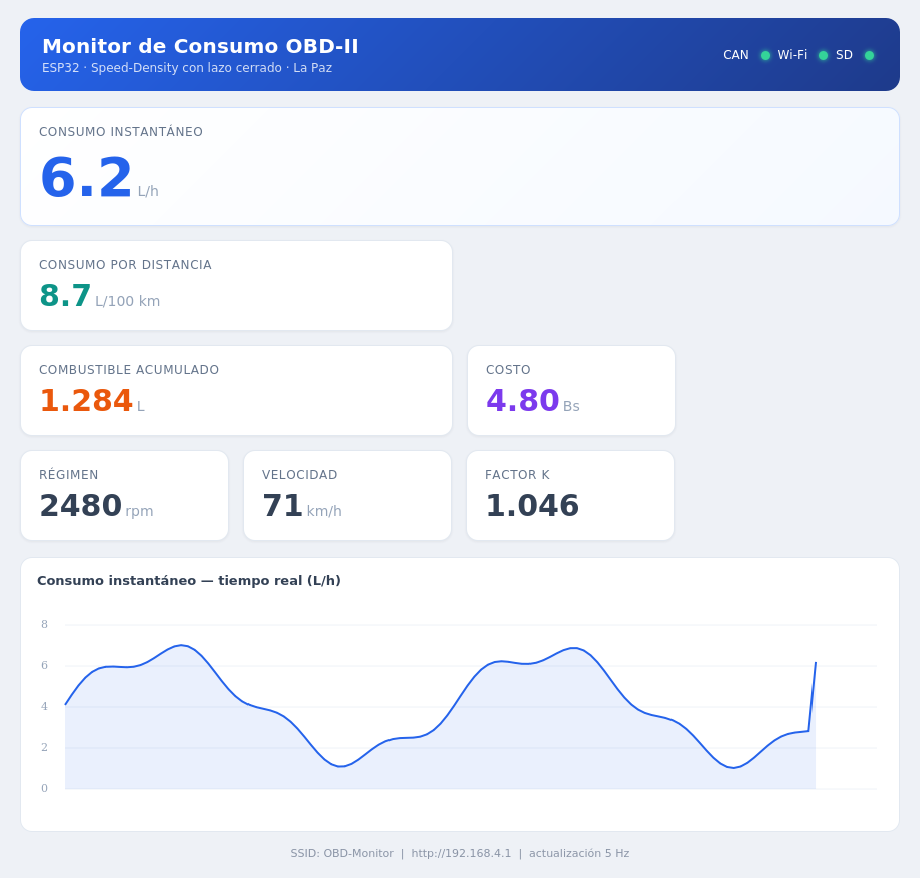
\includegraphics[width=0.75\textwidth]{Images/dashboard.png}
%
%	\vspace{4mm}
%	\small\raggedright
%	\textit{Nota.} Elaboración propia.
%	% Nota (APA): Elaboración propia.
%\end{figure}
%
%% ---------------------------------------------------------------------
%\subsection{Análisis de tiempos de respuesta y saturación de datos}
%\label{subsec:tiempos}
%
%La validez del sistema en tiempo real se sustenta en dos condiciones: que cada ciclo
%de adquisición quepa dentro de su periodo, y que ninguna cola ni canal se sature.
%
%\subsubsection{Presupuesto temporal del ciclo}
%
%La condición de tiempo real exige que el tiempo de ejecución del ciclo sea menor que
%el periodo asignado:
%
%\begin{equation}
%	T_\text{ciclo} + T_\text{cálculo} \;<\; T_\text{periodo},
%	\label{eq:presupuesto}
%\end{equation}
%
%donde $T_\text{ciclo}\approx 43\,\mathrm{ms}$ (Tabla~\ref{tab:tiempos-pid}),
%$T_\text{cálculo}<1\,\mathrm{ms}$ (operaciones en punto flotante e interpolación) y
%$T_\text{periodo}=250\,\mathrm{ms}$. El margen resultante es
%$250\,\mathrm{ms}-44\,\mathrm{ms}=206\,\mathrm{ms}$, equivalente a un
%\textbf{$82\pct$ de holgura}, suficiente para absorber latencias de ECU varias veces
%superiores a las típicas.
%
%\subsubsection{Saturación de colas y canal}
%
%La cola hacia la MicroSD no se satura mientras la tasa de producción sea menor que la
%de consumo:
%
%\begin{equation}
%	\lambda_\text{prod} = f_s = 4\ \text{muestras/s}
%	\;<\;
%	\mu_\text{consumo} = \frac{1}{\bar{T}_\text{escritura}},
%	\label{eq:cola}
%\end{equation}
%
%con $\bar{T}_\text{escritura}\approx 4{,}5\,\mathrm{ms/registro}$ (incluyendo el vaciado
%amortizado), lo que da $\mu\approx 220\,\mathrm{registros/s}\gg\lambda$. En consecuencia, la
%ocupación de la cola permanece cercana a~1 y el buffer de 32~no se llena.
%
%Para el canal WebSocket, el caudal de datos debe permanecer por debajo del ancho de
%banda del enlace Wi-Fi:
%
%\begin{equation}
%	S_\text{json}\cdot f_\text{web}\cdot N_\text{cli} \;<\; B_\text{Wi-Fi},
%	\label{eq:ws}
%\end{equation}
%
%con $S_\text{json}\approx 160\,\mathrm{bytes}$, $f_\text{web}=5\,\mathrm{Hz}$ y
%$N_\text{cli}$ clientes. Para $N_\text{cli}=4$ resulta
%$\approx 3{,}2\,\mathrm{kB/s}\approx 26\,\mathrm{kbps}$, muy por debajo del enlace; la limitación
%práctica es el número de estaciones que el punto de acceso del ESP32 admite con
%estabilidad (del orden de 4).
%
%\subsubsection{Instrumentación en firmware}
%
%Las métricas anteriores se miden directamente en ejecución
%(Figura~\ref{fig:cod-instr}): la latencia por PID con el temporizador de alta resolución,
%la ocupación de la cola con \texttt{uxQueueMessagesWaiting} y el margen de pila de
%cada tarea con \texttt{uxTaskGetStackHighWaterMark}. Estos valores se exponen por el
%puerto serie o el propio tablero, y constituyen la evidencia de validación.
%
%\begin{figure}[H]
%	\caption{Medicion de latencia, ocupacion de cola y margen de pila.}
%	\label{fig:cod-instr}
%	\begin{lstlisting}[language=C++]
%uint64_t t0 = esp_timer_get_time();     // microsegundos
%bool ok = obdRequest(pid) && obdRead(pid, buf, len, 60);
%uint64_t dt = esp_timer_get_time() - t0;// latencia del PID
%		
%uint32_t ocup = uxQueueMessagesWaiting(qLog);// ocupacion de la cola
%uint32_t pila = uxTaskGetStackHighWaterMark(NULL);// palabras libres min.
%uint8_t  cli  = WiFi.softAPgetStationNum();  // clientes Wi-Fi
%	\end{lstlisting}
%	
%
%\end{figure}
%
%La Tabla~\ref{tab:metricas} resume las métricas de validación con sus límites de
%diseño y el método de medición.
%
%\begin{table}[htbp]
%	\captionsetup{labelformat=simple, labelsep=newline, textfont=it, labelfont=bf, justification=raggedright, singlelinecheck=false}
%	\caption{Métricas de validación temporal y de saturación.}
%	\centering
%	\label{tab:metricas}
%	\begin{tabular}{@{}lll@{}}
%		\toprule
%		\rowcolor[rgb]{0.851, 0.851, 0.851}
%		\textbf{Métrica} & \textbf{Límite de diseño} & \textbf{Método de medición} \\
%		\midrule
%		Latencia por PID        & $<60\,\mathrm{ms}$ (timeout)        & \texttt{esp\_timer\_get\_time} \\
%		Tiempo de ciclo         & $<250\,\mathrm{ms}$ (periodo)       & acumulado por ciclo \\
%		Ocupación de cola       & $\ll 32$ ($\approx 1$)           & \texttt{uxQueueMessagesWaiting} \\
%		Margen de pila          & $>512\ \text{palabras}$           & \texttt{uxTaskGetStackHighWaterMark} \\
%		Caudal WebSocket        & $< B_\text{Wi-Fi}$               & Ec.~\eqref{eq:ws} \\
%		Clientes Wi-Fi          & $\le 4$                          & \texttt{softAPgetStationNum} \\
%		\bottomrule
%	\end{tabular}
%	
%	\vspace{2pt}
%	{\footnotesize\textit{Nota.} Elaboración propia.}
%\end{table}
%
%% ---------------------------------------------------------------------
%\subsection{Gestión de errores y robustez del sistema}
%\label{subsec:robustez}
%
%El firmware incorpora tres mecanismos de tolerancia a fallos, complementados por
%indicadores LED de estado en la PCB (alimentación, CAN activo, MicroSD y Wi-Fi).
%
%\textbf{Perro guardián (watchdog).} El temporizador watchdog de tareas (TWDT) del
%ESP32 vigila la tarea de adquisición. Si esta no se realimenta dentro del plazo
%configurado ---por ejemplo, porque el bus CAN quedó sin actividad y la tarea se
%bloqueó--- el TWDT reinicia el sistema, garantizando la recuperación autónoma
%(Figura~\ref{fig:cod-wdt}).
%
%\begin{figure}[H]
%	\caption{Configuracion del watchdog de tareas.}
%	\label{fig:cod-wdt}
%	\begin{lstlisting}[language=C++]
%esp_task_wdt_init(5, true);   // plazo 5 s; reinicia si vence
%esp_task_wdt_add(NULL);       // suscribe la tarea actual (adquisicion)
%// ... y dentro del lazo:  esp_task_wdt_reset();
%	\end{lstlisting}
%	
%
%\end{figure}
%
%\textbf{Recuperación de bus-off.} El controlador CAN entra en estado \emph{bus-off}
%cuando su contador de errores de transmisión (TEC) supera 255, desconectándose del
%bus \citep{bosch1991can}. El firmware detecta este estado y dispara la recuperación
%automática (Figura~\ref{fig:cod-busoff}); los contadores TEC/REC se monitorean para
%registrar la degradación antes de llegar a ese punto.
%
%\begin{figure}[H]
%	\caption{Deteccion y recuperacion de bus-off (TWAI).}
%	\label{fig:cod-busoff}
%	\begin{lstlisting}[language=C++]
%void canCheckHealth() {
%	twai_status_info_t st;
%	twai_get_status_info(&st);
%	if (st.state == TWAI_STATE_BUS_OFF) {
%		twai_initiate_recovery();        
%		// recupera tras 128x11 bits recesivos
%	} else if (st.state == TWAI_STATE_STOPPED) {
%		twai_start();   // reanuda tras recuperacion
%	}
%	// st.tx_error_counter 
%	// st.rx_error_counter > 96 -> registrar alerta
%}
%	\end{lstlisting}
%	
%
%\end{figure}
%
%\textbf{Estrategia de respaldo (fallback).} Si la ECU no responde durante varios
%ciclos consecutivos (superando un umbral configurable), la muestra se marca como
%inválida: el sistema conserva el último factor $K$ y la última curva $\eta_v$ válidos,
%mantiene en pantalla la última estimación fiable señalándola como no actualizada, y
%registra el evento. De este modo nunca se publican valores corruptos ni se pierde la
%calibración aprendida. La Tabla~\ref{tab:errores} sintetiza la matriz de errores.
%
%\begin{table}[H]
%	% Formato APA 7
%	\captionsetup{labelformat=simple, labelsep=newline, textfont=it, labelfont=bf, justification=raggedright, singlelinecheck=false}
%	\caption[Matriz de gestión de errores del sistema]{Matriz de gestión de errores del sistema embebido.}
%	\label{tab:errores}
%	\centering
%	
%	\vspace{2mm}
%	% Ampliamos los anchos de columna para evitar el amontonamiento de texto (Total ~14.5 cm)
%	\begin{tabular}{@{} p{3.5cm} p{3.5cm} p{4.5cm} p{3.0cm} @{}}
%		\toprule
%		\rowcolor[rgb]{0.851, 0.851, 0.851}
%		\textbf{Condición} & \textbf{Detección} & \textbf{Acción} & \textbf{Estado resultante} \\
%		\midrule
%		Sin respuesta de un PID & Timeout en \texttt{WAIT} ($>60\,\text{ms}$) & Descartar trama, reintentar en el siguiente ciclo & Operación normal \\
%		\addlinespace
%		Pérdida prolongada de CAN & $n$ ciclos sin respuesta & Marcar dato inválido, conservar $K$ y $\eta_v(N)$ & Modo degradado \\
%		\addlinespace
%		Bus-off del controlador & TWAI STATE BUS OFF & \texttt{twai\_initiate()} & Recuperación automática \\
%		\addlinespace
%		Tarea bloqueada & TWDT vence ($5\,\text{s}$) & Reinicio del sistema & Rearranque limpio \\
%		\addlinespace
%		Fallo de MicroSD & Error al abrir o escribir & Continuar sin registro, alertar por LED & Operación sin log \\
%		\bottomrule
%	\end{tabular}
%	
%	\vspace{4mm}
%	\small\raggedright
%	\textit{Nota.} Elaboración propia. La matriz detalla las contingencias consideradas en el diseño del firmware para asegurar la continuidad de la adquisición de datos de la ECU.
%\end{table}
%
%En conjunto, el diseño de software materializa el modelo en lazo cerrado sobre una
%arquitectura concurrente de dos núcleos, con subsistemas desacoplados, presupuesto
%temporal verificable y mecanismos de recuperación autónoma, satisfaciendo los
%requisitos de determinismo, robustez y confiabilidad del proyecto.
%
%\subsection{Gestión de energía y modo de reposo}
%\label{subsec:energia}
%
%El conector OBD-II mantiene el pin~16 con tensión de batería ($+12$~V) de forma
%permanente, incluso con el vehículo apagado. Por ello, un módulo conectado de forma
%fija queda energizado las 24~horas y, de no gestionarse su consumo, puede descargar
%gradualmente la batería. Esta subsección describe la estrategia para que el sistema
%entre en un modo de reposo de muy bajo consumo cuando el vehículo no está en uso y se
%reactive automáticamente al volver a encenderse.
%
%\subsubsection{Detección del vehículo inactivo}
%
%La detección se apoya en la actividad del bus CAN: mientras el contacto está activo, el
%bus presenta tráfico constante de las distintas ECU; al apagar el vehículo, el bus
%entra en reposo y deja de transmitir tramas tras unos minutos. El firmware aprovecha
%este comportamiento: si no se recibe ninguna trama válida durante un intervalo
%$T_\mathrm{idle}$ (por ejemplo, 90~s), concluye que el vehículo está apagado y procede
%a suspenderse. Como criterio complementario puede emplearse la tensión de la batería
%(con el motor en marcha el alternador la eleva a unos 14~V, frente a $\sim$12{,}4~V con
%el motor apagado), leída mediante un divisor resistivo.
%
%\subsubsection{Modos de bajo consumo del ESP32}
%
%El ESP32 ofrece varios modos de energía con distinto compromiso entre consumo y
%latencia de reactivación (Tabla~\ref{tab:modos-energia}). Para el reposo se selecciona
%el \emph{deep-sleep}, que reduce el consumo del microcontrolador a una fracción ínfima
%del de operación, a costa de reiniciar la ejecución al despertar ---lo cual es
%compatible con la persistencia en MicroSD ya implementada, que recupera el factor $K$
%y la curva $\eta_v$ tras cada arranque \citep{espressif_sleep}.
%
%\begin{table}[htbp]
%	\captionsetup{labelformat=simple, labelsep=newline, textfont=it, labelfont=bf, justification=raggedright, singlelinecheck=false}
%	
%	\caption{Modos de energía del ESP32 y su aplicación.}
%	\label{tab:modos-energia}
%	\centering
%	\begin{tabular}{@{}llll@{}}
%		\toprule
%		\rowcolor[rgb]{0.851, 0.851, 0.851}
%		\textbf{Modo} & \textbf{Consumo típico} & \textbf{Estado retenido} & \textbf{Reactivación} \\
%		\midrule
%		Activo (Wi-Fi activo)   & $\sim$150 mA          & completo              & inmediata \\
%		Activo (Wi-Fi inactivo) & $\sim$30 mA           & completo              & inmediata \\
%		Light-sleep             & $\sim$0{,}8 mA        & RAM y periféricos     & microsegundos \\
%		\textbf{Deep-sleep}     & $\sim$10 $\mu$A       & solo memoria RTC      & reinicio (\texttt{setup}) \\
%		\bottomrule
%	\end{tabular}
%\end{table}
%
%\subsubsection{Suspensión y reactivación}
%
%Antes de dormir, el firmware persiste la calibración, detiene el controlador TWAI y
%coloca el transceptor SN65HVD230 en modo \emph{standby} a través de su pin RS, lo que
%reduce su consumo a unos $0{,}2~\mu$A manteniendo la vigilancia del bus. Acto seguido
%configura las fuentes de despertar y entra en deep-sleep (Figura~\ref{fig:cod-sleep}).
%La fuente principal es la actividad del bus CAN: la línea RXD del transceptor
%se conecta a un GPIO con capacidad de despertar externo (\texttt{ext0}), de modo que la
%aparición de un bit dominante ---cuando el vehículo se enciende y el bus se reactiva---
%despierta al ESP32. Como respaldo se programa un despertar periódico por temporizador
%RTC que sondea brevemente el bus y vuelve a dormir si no detecta actividad. La
%Figura~\ref{fig:energia-fsm} resume la transición entre ambos modos.
%
%\begin{figure}[htbp]
%	\caption[Entrada en reposo profundo y despertar por actividad del bus]{Entrada en reposo
%		profundo y despertar por actividad del bus.}
%	\label{fig:cod-sleep}
%	\begin{lstlisting}[language=C++]
%#include "esp_sleep.h"
%#define WAKE_PIN  GPIO_NUM_4     // RXD del transceptor 
%#define T_IDLE_MS 90000          // 90 s sin tramas 
%
%uint32_t lastFrameMs = 0; // marca de la ultima trama recibida
%		
%void goToDeepSleep() {
%	saveK();              // persistir calibracion en MicroSD
%	twai_stop(); twai_driver_uninstall(); // liberar el controlador
%	digitalWrite(CAN_RS, HIGH); // SN65HVD230 -> standby (~0.2 uA)
%	// despertar cuando el bus vuelva a estar activo 
%	esp_sleep_enable_ext0_wakeup(WAKE_PIN, 0);
%	// respaldo: sondeo periodico cada 5 min
%	esp_sleep_enable_timer_wakeup(5ULL * 60 * 1000000);
%	esp_deep_sleep_start();      // ~10 uA hasta el despertar
%}
%
%// En el lazo principal, tras cada ciclo de adquisicion:
%//   if (millis() - lastFrameMs > T_IDLE_MS) goToDeepSleep();
%	\end{lstlisting}
%\end{figure}
%
%\begin{figure}[htbp]
%	
%	\caption{Transición entre el modo de operación y el modo de reposo de bajo consumo del
%		módulo, gobernada por la actividad del bus CAN.}
%	\label{fig:energia-fsm}
%	\centering
%	\vspace{2pt}
%	\resizebox{0.82\textwidth}{!}{%
%		\begin{tikzpicture}[
%			font=\normalsize,
%			base/.style={rectangle, draw, rounded corners, line width=0.8pt, align=center,
%				minimum height=1.5cm, minimum width=3.4cm},
%			act/.style={base, draw=green!60!black, fill=green!15},
%			slp/.style={base, draw=blue!70!black, fill=blue!12},
%			line/.style={-{Latex[length=2.8mm]}, line width=1.0pt, draw=black!75},
%			lbl/.style={font=\small, fill=white, inner sep=2.5pt, align=center}
%			]
%			\node[act] (act) {\textbf{ACTIVO}\\[2pt]\footnotesize adquisición + cálculo + web};
%			\node[slp, right=6.2cm of act] (slp) {\textbf{REPOSO}\\[2pt]\footnotesize deep-sleep ($\sim$10 $\mu$A)};
%			\draw[line] (act.north) .. controls +(0,1.2) and +(0,1.2) ..
%			node[lbl, above] {sin tráfico CAN $>$ $T_\mathrm{idle}$\\(detener TWAI, transceptor a standby)} (slp.north);
%			\draw[line] (slp.south) .. controls +(0,-1.2) and +(0,-1.2) ..
%			node[lbl, below] {actividad en el bus CAN (RXD)\\$\rightarrow$ despertar y reiniciar} (act.south);
%		\end{tikzpicture}%
%	}
%
%	% Nota (APA): Elaboración propia.
%\end{figure}
%
%\subsubsection{Presupuesto de energía y justificación del modo deep-sleep}
%
%Con el ESP32 en deep-sleep ($\sim$10~$\mu$A) y el transceptor SN65HVD230 en standby
%($\sim$0{,}2~$\mu$A), el consumo en reposo queda dominado por la corriente de
%	reposo (IQ) del convertidor TPS54331, del orden de $\sim$2{,}5~mA. El consumo
%acumulado durante el período máximo de inactividad del vehículo ---estimado en
%\textbf{3 días}--- se calcula como:
%
%\begin{equation}
%	Q_\mathrm{reposo} = I_\mathrm{reposo} \times t_\mathrm{max}
%	= 2{,}5\,\mathrm{mA} \times 72\,\mathrm{h} = 180\,\mathrm{mAh}.
%	\label{eq:q-reposo}
%\end{equation}
%
%Referida a la capacidad nominal de una batería de automóvil típica (45~Ah), esta
%energía representa:
%
%\begin{equation}
%	\frac{Q_\mathrm{reposo}}{C_\mathrm{bat}} =
%	\frac{180\,\mathrm{mAh}}{45{,}000\,\mathrm{mAh}} \approx 0{,}4\,\%.
%	\label{eq:porcentaje-bat}
%\end{equation}
%
%Un $0{,}4\,\%$ de la capacidad de la batería es prácticamente despreciable,
%especialmente considerando que el propio vehículo ya presenta corrientes parásitas en
%reposo de 20--50~mA (reloj, alarma, ECUs en standby), frente a los cuales los
%2{,}5~mA del módulo representan una fracción menor. Además, al volver a encenderse, el
%alternador recupera esos 180~mAh en cuestión de minutos de marcha. En consecuencia,
%el modo deep-sleep del ESP32 es suficiente para el caso de uso del presente
%	proyecto, sin necesidad de modificación de hardware. La desconexión completa del rail
%de 3{,}3~V (power-gating del convertidor buck) se plantea como recomendación para
%versiones futuras del módulo en escenarios de inactividad prolongada.
%
%La Tabla~\ref{tab:energia} consolida el presupuesto de energía comparando los tres
%escenarios posibles.
%
%\begin{table}[htbp]
%	\captionsetup{labelformat=simple, labelsep=newline, textfont=it, labelfont=bf, justification=raggedright, singlelinecheck=false}
%	
%	\caption{Presupuesto de energía en operación y en reposo.}
%	\label{tab:energia}
%	\centering
%	\resizebox{\textwidth}{!}{%
%		\begin{tabular}{@{}p{3.8cm}ccccl@{}}
%			\toprule
%			\rowcolor[rgb]{0.851, 0.851, 0.851}
%			\textbf{Estado} & \textbf{ESP32} & \textbf{Transc.}
%			& \textbf{TPS54331 IQ} & \textbf{Total@bat.} & \textbf{3 días acum.} \\
%			\midrule
%			Operación (adq.+Wi-Fi)
%			& $\sim$150 mA & $\sim$5 mA & $\sim$0{,}12 mA & $\sim$50 mA$^{\dagger}$ & --- \\[4pt]
%			\textbf{Reposo (deep-sleep)}
%			& 10 $\mu$A & 40 $\mu$A & 116 $\mu$A$^{*}$
%			& $\sim$\textbf{0{,}14 mA} & \textbf{10 mAh (0,02\,\%)} \\[4pt]
%			Reposo + power-gating
%			& apagado & apagado & apagado & $<$20 $\mu$A & $<$1{,}5 mAh \\
%			\bottomrule
%		\end{tabular}}
%	
%	\vspace{4pt}
%	{\footnotesize
%		$^{*}$ IQ típico del TPS54331DR según hoja de datos de Texas Instruments;
%		valor a verificar por medición directa del módulo ensamblado.\\
%		$^{\dagger}$ Corriente desde batería (12~V): $P_\mathrm{out}/(V_\mathrm{bat}\times\eta)
%		= (3{,}3\,\mathrm{V}\times155\,\mathrm{mA})/(12\,\mathrm{V}\times0{,}85)\approx50\,\mathrm{mA}$.
%		El porcentaje de capacidad se calcula respecto a una batería de 45~Ah.}
%\end{table}
%En conjunto, el diseño de software materializa el modelo en lazo cerrado sobre una
%arquitectura concurrente de dos núcleos, con subsistemas desacoplados, presupuesto
%temporal verificable, gestión de energía en reposo y mecanismos de recuperación
%autónoma, satisfaciendo los requisitos de determinismo, robustez, eficiencia energética
%y confiabilidad del proyecto.